  %-----------
% thesis.tex
%-----------
% This is a template which hopefully is useful to anyone putting together their
% thesis.  It is usually a good idea to have one main file (such as this) which
% includes all your chapters.  That way you can work on separate chapters
% without having to compile your whole thesis.  I would also recommend not
% calling your files chap1.tex, chap2.tex etc., since you are bound to want to
% change the order around, and then the numberings will just cause confusion!
% Questions/comments  should be sent to to george.stagg@ncl.ac.uk
%------------------------------------------------------------------------------

%------------------------------------------------------------------------------
% Set the class and font size.  The article class does not allow chapters, so
% you'll want to avoid that.  I used 11pt for final submission.
\documentclass[twoside, openright, 12pt]{report}
%------------------------------------------------------------------------------

%------------------------------------------------------------------------------
% Set the left and right margins.  Remember, you will need to leave more space
% on the left, to allow for binding, when it comes to submission.  You can
% easily change the margins as you like, but I think there must be at least a
% 30mm margin on the binding edge.
%
% One-sided A4 (A one-sided version is good to take into the viva for making notes)
%\usepackage[a4paper,left=35mm,right=25mm,top=40mm,bottom=35mm]{geometry}
%
% Two-sided A4 (Use this for the final offical binding/submission)
\usepackage[a4paper,twoside,left=35mm,right=25mm,top=40mm,bottom=35mm]{geometry}
%
% Centred A4
%\usepackage[a4paper,left=30mm,right=30mm,top=40mm,bottom=35mm]{geometry}
%
% Two-sided smaller book sized
%\usepackage[papersize={6in,9in},twoside,left=0.75in,right=0.5in,top=0.5in,bottom=0.5in,includehead, includefoot]{geometry}
%------------------------------------------------------------------------------

%------------------------------------------------------------------------------
% Uncomment the two lines below if you would prefer blank lines for paragraph
% breaks, rather than indents.
%\setlength{\parindent}{0em}
%\setlength{\parskip}{1ex}
%------------------------------------------------------------------------------

%------------------------------------------------------------------------------
% This line prevents LaTeX complaining about \headheight being too small.
\setlength{\headheight}{15pt}
%------------------------------------------------------------------------------

%------------------------------------------------------------------------------
% If you only want to include certain chapters in the final output, do
% something like the commented line below.  Note that the entire document must
% have been compiled at least once for references to work correctly.
%\includeonly{chapter}
%------------------------------------------------------------------------------

% The masthesis style file itself.  Many additional packages are already
% defined in the style file (inputs/masthesis.sty).  Either add your own
% packages there, or below the following line.
\usepackage{masthesis}
% One-and-a-half or double-line spacing.  I used 1.5 for final submission.
\onehalfspacing
%\doublespacing
%% includeonly{relevant-chapter}  - comment out for full thesis
%\includeonly{
% chapters/intro,
% chapters/background,
% chapters/conclusion
% chapters/ds-for-ow
% }

\begin{document}

  \phdtitle{Uncertainty Quantification for Stochastic Simulators with Application to Offshore Wind Farms} % Title.
           {Jack Callum Kennedy}          % Author.
           {fig/logo}                   % Graphic for the title page.
           {December 2022}                % Date.

  \thispagestyle{empty}
  \cleardoublepage

  %\input{dedication}                    % Optional dedication.
  \section*{Declaration}
I declare this thesis is my own reasearch and unless explicity stated, the writing, research and code used to implement methods is my own.

The Athena model was developed at the University of Strathclyde, apart from the modifications required to implement a spare parts strategy in section 2.1.1, which are my own.

Parts of Chapters 4 and 5 have been published in the Journal of the Royal Statistical Society, Series C (Applied Statistics) \citet{Kennedy2023}. This paper was co-authored by my supervisors, Kevin Wilson and Daniel Henderson, however the research and novel ideas are my own.

This thesis has not been submitted for examination at another university.


  
\thispagestyle{empty}
\clearpage

\vspace*{\stretch{2}}

\begin{center}
  \textbf{Acknowledgements}\\[0.75cm]

  \begin{minipage}{0.9\textwidth}
    \setlength{\parskip}{0.45em}
There are lots of people I am grateful for. Here are some select highlights.

First of all, I'd like to acknowledge the EPSRC for making this entire thing financially viable. Spending over $20$ years in formal education is simultaneously a badge of honour but also a source of crippling pain. Because of you, EPSRC, I've been able to enjoy the experience of not paying council tax until my mid-to-late twenties. The downside of this arrangement is my grandparents have been asking, with minimal optimism, ``Jack, are you \emph{ever} going to get a job?''.

A massive thank you to my PhD supervisors, Kevin Wilson and Daniel Henderson. Without the pair of you this thesis would be littered with typos are \emph{even more} of my bad jokes. Kevin, I've enjoyed our many, excessively long conversations about the way statistics should be done. I'm not sure if anyone else really agrees with us. Daniel, thank you for keeping me \emph{and Kevin} on track.

To everyone who has held a desk in PhD 4, it's been good (apart from chaotic bit where going in the office was banned). It would be unjust if I did not recognise Jack as a door sign aficionado and the world's most effective rubber duck.

I'd also like to thank my friends in the Royal Statistical Society, especially the Young Statisticians, for reminding me that statistics is something I actually enjoy, even when this thesis has convinced me otherwise.

My friends outside of statistics should also be mentioned. I am grateful that you have pretended to be interested in my thesis, doing a PhD becomes an annoying personally trait which is hard to shake off. Jack, Tom, I have always assumed that ``massive nerd'' is a term of endearment.

Finally, Aim\'ee, thank you for everything you have done for me. Putting up with me being in a right strop on many occasions for reasons such as my code crashing for the fifth time in as many hours, or because reviewer 2 has been particularly unforgiving. Without your love and support this would have been much more difficult.

  \end{minipage}

\end{center}

\vspace*{\stretch{3}}

\cleardoublepage
                   % Acknowledgements.

  \begin{abstract}
Computationally expensive computer models, known as simulators, are fundamental to the modern scientific process. In recent years, there has been an increased interest in \emph{stochastic simulators} as analysts aim to model uncertainty in their predictions. Stochastic simulators are found in all areas of science. We focus on a particular simulator, known as the Athena simulator, which is used to assess the performance of offshore wind farms in their early life.

Athena is typical of many stochastic simulators in that it can take a long time to run and the variance exhibited by the simulator may depend on the simulator input. This poses multiple computational challenges for subjective Bayesians who wish to perform computer-intensive tasks such as sensitivity analysis or decision support. A common solution to the large computational cost of such analyses is to construct a fast statistical surrogate model, known as an \emph{emulator}, to produce an efficient approximation to the simulator with an appropriate quantification of uncertainty. Two popular emulators for stochastic simulators, HomGP, the homoscedastic Gaussian process, and HetGP, the heteroscedastic Gaussian process.

The first contribution of this thesis is the proposition of a method, based upon \citet{Kennedy2000}, which seeks to exploit fast approximations to stochastic simulators. We apply the general methodology to the Athena model in particular to construct an improved emulator. The approach considers an autoregressive structure for different `levels' of a simulator. We name the new approach stochastic multilevel emulation. \correction{The second contribution of this thesis is investigating algorithms to fit HetGP emulators. Many Bayesian emulators require computationally intensive methods such as Markov chain Monte Carlo to quantify uncertainty about emulator parameters. We recommend using a conjugate prior for HetGP which provides further computational savings and allows for tractable uncertainty quantification about emulator parameters}. Our Bayesian HetGPs are used to perform a sensitivity analysis as preparation for expert elicitation for parameters in the Athena simulator. The final contribution of this thesis is combining two distinct approaches. We show, via Bayesian Optimisation and History Matching, that decision making and decision support approaches can work in harmony. We apply this novel approach to construct a set of feasible solutions to a resource allocation problem within an offshore wind farm.
\end{abstract}
                      % Abstract.

  \pagenumbering{roman}                 % Change the page numbering style for
                                        % Table of Contents and Lists.

  \tableofcontents
  \listoffigures
  \listoftables
  \listofalgorithms

  \clearpage                            % End the current page making sure all
  \thispagestyle{empty}                 % tables/figures are printed.
  \cleardoublepage                      % Necessary for correct page numbering.

  \pagenumbering{arabic}                % Reset the page numbering style.

  %% chapters

  \begin{chapter}{Introduction \label{Ch:Intro}}
\section{Motivation: computer experiments}
Historically, science was undertaken almost exclusively via physical experiments. In search of new knowledge, the scientific community did many unusual, and sometimes dangerous, things. Marie Curie's experimentation with X-rays almost surely led to her premature death, Ernest Rutherford (or rather, his students, Hans Geiger and Ernest Marsden), sat in dark rooms for hours in order to prove that atoms are indeed divisible, and to investigate the feasibility of cryonics, \citet{Smith1954} froze hamsters and reanimated them using microwaves.

The scientific process has since evolved. We have developed ethical standards for the types of experiments we are allowed to perform, as well and health and safety protocols. A key advancement has been the development of mathematical and statistical modelling to predict what may happen in complex systems. Such models take inputs, $\bx$, transform them through a function, $f(\cdot)$, and produce an output, $y = f(\bx)$. The function $f(\cdot)$ may encode our understanding of a physical process via a set of complex equations and $\bx$, the parameter settings, may represent a hypothetical scenario. Evaluating $f(\cdot)$ at many values of $\bx$ allows a scientist to ask many ``what if'' questions, at a fraction of the cost of running an equivalent physical experiment. The function $f(\cdot)$ is usually intractable, thus must be evaluated via a computer code. We refer to a computer code as a \textit{simulator}. Typical simulators can be of the order of hundreds, or even thousands, of lines of code. Answering these ``what if'' questions via a computer is what we might term a \textit{computer experiment}. Within the biological community, this form of experiment is sometimes termed an \textit{in silco} experiment.

In many engineering contexts, such as the generation of energy, we encounter physical systems that are incredibly complex. An engineer may want to optimise parameters of these systems, or simply explore what would happen under many ``what if'' scenarios. Performing physical experiments on gas distribution networks, full scale nuclear power plants, or offshore wind farms located miles away from the coast is not a straightforward task. Even if these experiments were financially feasible, the experiments would undoubtedly take \textit{a very long time}.

Using a computer simulation to mimic a physical system is no panacea. Despite modern computing capabilities, it is typical of many computer simulators to have long run times. Exactly what `long' means is context-dependent, but the Athena simulator \citep{Zit13, Zit16, Zit2021}, used throughout this thesis, has typical run times of $5$ minutes for a single parameter setting on a modern desktop computer. A $5$ minute run time might be acceptable for making a handful of runs, but becomes problematic when we want to make thousands of runs. A more extreme example is HadCM3 --- the climate model used by the MET office --- run times are in excess of a week for a single parameter setting \citep{Domingo2020}.

Despite the advantages of using a model in place of physical experiments, we must always remind ourselves that the model is exactly that. It is a model. An imperfect representation of the physical system it aims to mimic.

\subsection{The role of statistical thinking in computer experiments}

Statistics has made, and continues to make, contributions to computer experiments and the wider field of Uncertainty Quantification (UQ). The main role of statistics in this field is the development and application of surrogate models known as \textit{emulators} \citep{Ohagan01, Vernon14}. Emulators take a set of inputs $X$ and evaluations of the simulator at those inputs $\by = f(X)$, to construct a statistical model typically several orders of magnitude faster to run than the original simulator \citep{Salter2016}. The statistical model is an approximation to the simulator, thus an appropriate quantification of uncertainty is attached to the emulator's point predictions.

Statistical thinking does not just allow us to perform efficient prediction, and besides, prediction for its own sake is rarely the objective of a simulator. We typically develop simulators as a means to perform another task, such as optimisation, inference, calibration or decision analysis. Phrasing the use of a complex simulator in statistical terms has lead to many developments. A popular example is \textit{Bayesian Optimisation}, where ideas from statistical decision theory allow us to optimise expensive simulators with relatively few runs of the simulator \citep{Frazier2018}. Sampling schemes such as Latin Hypercubes \citep{Mckay1979}, allow us to construct designs for simulation experiments which cover the input space efficiently which eases the task of emulation. Elicitation and subjectivism allow us to consider model discrepancy and thus allow us to calibrate simulators to observational data, whilst allowing for the fact that the simulator (and emulator) are imperfect representations of a corresponding physical system \citep{Ohagan01, Vernon2022}.

\section{Contributions}
\subsection{Stochastic multilevel emulation}
The first main contribution is the development an emulator that we call a stochastic multilevel (SML) emulator. The SML emulator combines two established approaches; HetGP and multilevel emulation.

HetGP \citep{Goldberg1998, Binois2018} is a data-hungry model, which is otherwise well suited to the emulation of stochastic simulators. It uses a pair of GP emulations to construct flexible mean and variance estimates for stochastic simulators. Multilevel emulation leverages the fact that many simulators can be run at varying levels of complexity, and thus we have a more accurate simulator at higher `levels'. The more accurate/complex the simulator is, the longer it takes to run. The multilevel emulator \citep{Kennedy2000}, finds a way to combine runs from different levels of \textit{deterministic} code, to provide improved predictions of the most expensive level of code. Our SML emulator combines these two approaches to enable us to use cheap versions of a stochastic simulator to construct improved predictions for a more expensive version. We also consider several estimation techniques for HetGP and SML, and find a computationally efficient way to incorporate prior information into both HetGP and SML emulators.

\subsection{A decision support framework for offshore wind}
Our second main contribution is the development of a decision support framework using stochastic simulators. This is an extension of the decision support frameworks given in \citet{Lawson2016} and \citet{Owen2020} who study deterministic simulators. The core idea in decision support is to find decisions (model inputs) which are within a given tolerance of some approximately optimal reference value. Our application has several novel ideas; firstly we discuss how decision making and decision support can be brought closer together via Bayesian optimisation and history matching. Our application also has a challenging feature; a subset of our simulator inputs form a discrete simplex. Within the computer experiments literature, inputs are usually formed on a hypercube. We discuss a method for generating uniformly distributed samples from the discrete simplex which are within tolerance of the reference value. We also consider post-processing of the uniform samples to improve the space-filling properties of a design for a multi-wave computer experiment.

\section{Thesis outline}

In \cref{Ch:background} we introduce the Athena simulator, a complex, stochastic simulator used to model the behaviour of a large offshore wind farm. The purpose of the Athena simulator is to aid decision making under uncertainty. This uncertainty is decomposed into two parts. Firstly, aleatory uncertainty; the inherent randomness of the world. The second is epistemic uncertainty; we represent this mathematically via a (prior) probability distribution. Athena employs a large and complex prior probability distribution over many unknown quantities for which there is little or no relevant data available; many relate to the lifetime distributions of critical components in Athena.

Probability elicitation is important within Athena as many of the parameters are uncertain and thus are represented in the Athena simulator by an expert's prior distribution. We want to propagate the uncertain parameters through the Athena simulator to understand how input uncertainty induces output uncertainty. We therefore discuss some core concepts from probability elicitation. Since Athena is used to help make operation and maintenance decisions within an offshore wind setting, we also provide an introduction to Bayesian decision analysis and utility theory; a framework for making decisions.

The use of computationally expensive models makes analyses relying on many evaluations of $f(\bx)$ extremely computationally expensive. Such analyses include uncertainty analysis or decision analysis. In \cref{Ch:Emulators}, we introduce the notion of an \textit{emulator}. Emulators are fast, statistical approximations to complex computer simulators. Emulators repurpose and adapt regression techniques to produce approximations to complex computer simulators.

In \cref{Ch:Hetsml}, we describe the heteroscedastic Gaussian Process (HetGP) as a way to emulate stochastic computer models which exhibit input-dependent noise. We develop a general approach for SML emulation, which uses different versions of a simulator to improve the final emulator. Finally, we compare some estimation methods for HetGP and SML via an application to the Athena simulator.

We return to probability elicitation in \cref{Ch:sensitivity}. In particular, we perform a probabalistic sensitivity analysis of the Athena simulator. This is facilitated by the HetGP and SML emulators fitted in \cref{Ch:Hetsml}.

\cref{Chap:optimisation} marks a change of direction in the thesis. We review some common optimisation approaches with a view towards decision making (which can be expressed as an optimisation problem). We then discuss how emulators can be incorporated into the optimisation process. We consider some practical differences between \textit{making} decisions and \textit{supporting} decision making. We motivate the use of history matching inspired techniques as an appropriate method for facilitating decision support. Finally, we discuss algorithms for generating sets of decisions that are consistent with an approximately optimal decision.

In \cref{Ch:ds-for-ow}, we put into practice some of the techniques described in \cref{Chap:optimisation}. The optimisation techniques are used to maximise the expected utility function which depends on the output of Athena. We utilise techniques given in \citet{Owen2020} and extend them to the stochastic case. We also consider the problem of generating decisions on a subset of a discrete simplex; this is a nonstandard problem within the uncertainty quantification literature.

The thesis is drawn to a close in \cref{Ch:conclusions}. We review the findings of this thesis and provide future research avenues.
\end{chapter}

  \begin{chapter}{Background \label{Ch:background}}
This thesis aims to develop tools to aid computationally expensive analyses that a subjective Bayesian may perform. These computationally expensive tasks usually amount to computing $Y = f(\bX)$ where $f(\cdot)$ is an expensive to evaluate function, which is thought to be highly non-linear, $\bX$ is an uncertain vector of inputs to $f(\cdot)$ and $Y$ is the (uncertain) quantity of interest. We consider two concrete instances of such a problem.

The first problem we consider is a sensitivity analysis to aid the elicitation of $\bX$. The sensitivity analysis relies on calculating the intractable integrals $\E_X\{f(\bX)\}$, $\var_X \{f(\bX)\}$, as well as conditional expectations and variances, such as $\E_{X_i} \{  \var_{\bX_{-i}}(f(X) \mid X_i) \}$, where $\bX_{-i}$ denotes all elements of $\bX$ apart from the $i$th element. This in turn relies on evaluation of $f(\bx)$ for many values of $\bx$. The word `many' is somewhat vague, but we would expect that evaluating $f(\cdot)$ at somewhere in the region of $10^4$ -- $10^6$ unique input configurations to be necessary to obtain accurate estimates of the required expectations and variances.

The second problem we consider is decision analysis, in which we elicit a function of the form $U(\bx) = \E_{\btheta} \{ u(\bx, \btheta) \}$ where $\btheta$ is a collection of unknown quantities, $\bx$ is the vector representing the decision to be made, and $u$ is a function which itself depends on $f(\bx)$. This problem is computationally intractable; evaluation of $U(\bx)$ is typically only achievable via Monte Carlo methods. This makes maximising $U(\bx)$ difficult because $U(\bx)$ itself cannot be computed exactly. The difficulty of an intractable decision analysis is increased when $U(\bx)$ is expensive to compute, which is a problem we have.

We will perform analyses on the computationally expensive Athena simulator, which is a stochastic model of an offshore wind farm \citep{Zit13, Zit16, Zit2021}. This chapter will consist of primers on the Athena simulator (\cref{sec:athena}), probability elicitation (\cref{sec:prob}), and  Bayesian decision analysis, including the elicitation of utility functions.

\section{The Athena simulator: a stochastic model of an offshore wind farm\label{sec:athena}}
% some information about the athena simulator
The Athena simulator \citep{Zit13, Zit16, Zit2021} is a point process model of a large offshore wind farm. The intended purpose of Athena is to aid decision making under uncertainty, as such, Athena does not model raw power output or take into account precise details of the wind, but aims to model the reliability of a wind farm using techniques from reliability analysis. The reason for not modelling raw output or including synthetic weather data is that they are highly uncontrollable and very uncertain, although their aggregate effects can be characterised much more precisely. We can however, make plausible predictions about the \textit{reliability} of the wind farm.

The Athena simulator generates predictions by simulating events within an offshore wind farm over a pre-specified time period $[0, T_{max}]$ years. There are many types of event that may happen within an offshore wind farm. Typical events include components breaking, components being repaired or replaced, and the deployment of boats to perform repairs. Other, less common, events may be the triggering of farm-wide maintenance, or turbines being switched on in the early stages of the wind farm's operational life.

To simulate events, the simulator starts from time $t=0$ and calculates the hazard function of each event possible at each time point over the period of interest; this is a function of time and the state of the wind farm. From this the ``total'' hazard (at each time point), known as the Force of Mortality (FOM), is calculated which then implies the next event time. If we are at $T_{p-1}$ then the time to the next event, $T_p$ is found as $R^{*}(T_p) = R^{*}(T_{p-1}) + E$ where $E \sim Exp(1)$ and $R^{*}$ is the cumulative intensity function of the wind farm. The use of an $Exp(1)$ random variable is justified by a general, theoretical result; see \citet{Pham2006} (Theorem $8.8$).

The event time $T_p$ is the deterministic solution to an integral which depends on the wind farm's current, stochastic, state.
The integral is
\begin{equation}
R^{*}(\tau_n) - R^{*}(\tau_{n-1}) = \int_{\tau_{n-1}}^{\tau_n} r^{*}(u) \, \textrm{d} u  \label{Eq:intensity}
\end{equation}
where $r^{*}$ is the wind farm's intensity function. If $\tau_{n-1}=T_{p-1}$ is the time of the last event, then $R^{*}(\tau_{n-1})$ is known. The goal is to find $R^{*}(\tau_n)$ by sequentially increasing $\tau_{n}$ to $T_{p-1} + \Delta t$, $T_{p-1} + 2\Delta t$, \ldots until $R^{*}(\tau_n) - R^{*}(\tau_{n-1}) > E$. The first value of $\tau_{n}$ satisfying the inequality is taken as $T_p$. Athena then decides which component caused the event. Events are typically subassemblies of a particular turbine failing or being repaired. The Athena simulator models the turbines as being constructed of $8$ main subassemblies and a $9$th `catch all' subassembly, which collectively models the behaviour of several less important subassemblies which together have a non-negligible effect. The subassemblies are the gearbox, generator, frequency converter, transformer, main shaft bearing, the blades, tower, foundations and the catch all.

Events are not caused only by subassemblies, for example, cables and transformers can fail and be repaired. Let $y_{j,k}(T_p)$ be an indicator taking the value $1$ when subassembly $(j,k)$ has failed and is $0$ otherwise. Let $\nu_{j,k}(T_p)$ be the failure intensity of subassembly $(j,k)$ and let $\mu_{j,k}(T_p)$ be the corresponding restoration intensity, then the probability that subassembly $(j,k)$ caused the event at time $T_p$ is
\begin{align}
  p_{j,k}(T_p) &= \frac{y_{j,k}(T_p)\nu_{j,k}(T_p) + (1-y_{j,k}(T_p))\mu_{j,k}(T_p)}{P + Q} \\
  P & =   \sum_{j,k} \left\{y_{j,k}(T_p)\nu_{j,k}(T_p) + (1-y_{j,k}(T_p))\mu_{j,k}(T_p)\right\}\nonumber\\
 Q &= \sum_l \left\{ y_{l}(T_p)\nu_{l}(T_p) + (1-y_{l}(T_p))\mu_{l}(T_p) \right\}\nonumber
\end{align}
where $y_l(T_p)$ is an indicator for the $l$th component which is not a subassembly, with failure intensity $\nu_l(T_p)$ and restoration intensity $\mu_l(T_p)$. The probabilities $\{y_{1,1}(T_p), y_{2, 1}(T_p), \ldots, y_1(T_p), y_2(T_p), \ldots \}$ form a partition of $[0,1]$, so drawing a $U(0,1)$ random variable allows us to simulate which event occurred. This is repeated until we reach the end of the pre-specified simulation period $T_{max}$.

The time to failure, $T_{j,k}$, of subassembly $j$ in turbine $k$ is modelled by a non-stationary Weibull distribution: $T_{j,k}\mid t \sim Weibull( \alpha_{j,k}(t), \kappa_{j,k}(t) )$. Recall that if $T$ is the time at which a component fails, then the survival function is $S(t) = \p (T > t)$, the hazard function is given by
\begin{align}
  h(t) &= \frac{-S'(t)}{S(t)}\\
  \iff  S(t) &=  \exp \left\{ -\int_0^t h(u) \, \textrm{d}  u \right\}.
\end{align}
We can then construct a Weibull distribution with time-dependent parameters by constructing a hazard function which changes form with time. In particular, a hazard function for a subassembly follows a `bathtub' curve which controls $\alpha_{j,k}(t)$ and $\kappa_{j,k}(t)$ . A bathtub hazard function corresponds to three phases of component life
\begin{itemize}
  \item[(i)] infant mortality (decreasing hazard)
  \item[(ii)] useful life (constant hazard)
  \item[(iii)] degradation  (increasing hazard).
\end{itemize}
Phase (i) corresponds to a period in which a larger than expected number of components fail due to manufacturing faults, or lack of operator experience. This is an important consideration when novel technologies and being employed in harsh environments, or existing technologies are employed in unfamiliar environments. Both of these scenarios are present within an offshore wind setting. In the next phase, the component works as expected; failures are caused only by external factors, such as extreme weather events damaging turbines or random operator error. Finally, components enter the degradation phase, in which components are starting to feel the effects of ageing, the components are becoming increasingly worn out with time and thus are increasingly likely to fail with time.

We can write a bathtub hazard function in the following form:
\begin{equation}
h(t) = \begin{cases}
        \alpha_0 \kappa_0 (\alpha_0 t)^{\kappa_0 - 1},& t \in [0, t_1)\\
        \alpha_1,& t \in [t_1,t_2)\\
        \alpha_2 \kappa_2 (\alpha_2 t)^{\kappa_2 - 1},& t \in [t_2, \infty) \\
       \end{cases}
\end{equation}
where $\kappa_0 < 1$, $\kappa_2 > 1$ and the constant hazard case ($h(t) = \alpha_1$) could be represented by $h(t) = \alpha_1 \kappa_1 (\alpha_1 t)^{\kappa_1 - 1}$ with $\kappa_1 = 1$, that is, exponentially distributed failure times. The hazard function is continuous so that $\alpha_0 \kappa_0 (\alpha_0 t_1)^{\kappa_0 - 1} = \alpha_1 = \alpha_2 \kappa_2 (\alpha_2 t_2)^{\kappa_2 - 1}$ and  In \cref{Fig:bathtub} we present an example  bathtub hazard function (left) with the corresponding survival function (right).
\begin{figure}
  \centering
  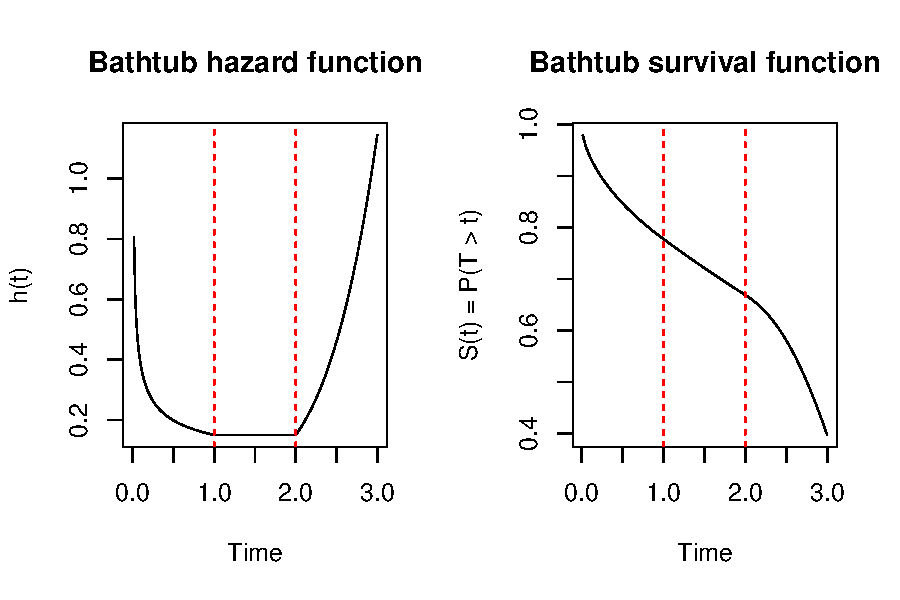
\includegraphics{fig-background/bathtub.pdf}
  \caption{An example of a bathtub hazard function (left) with the corresponding survival function (right). The dashed red lines indicate $t_1$ and $t_2$, the points in time when the nature of the hazard function changes. \label{Fig:bathtub}}
\end{figure}
Athena incorporates additional details into the hazard function. Performing maintenance tasks extends the expected life of a subassembly, whereas operator misuse decreases lifetimes, and the probability of operator misuse decreases with time, reflecting increased experience. A concept known as `virtual life' allows us to further manipulate $h(t)$. If we replace $t$ by $v(t)$, the virtual life, the hazard function, $h(v(t))$, can then reflect the state of the subassembly it models more accurately. We can think of $v(t)$ as the effective age of a component. Performing preventative maintenance should improve the lifespan of a component, thus it is effectively a `newer' component than prior to maintenance \citep{Finkelstein2007}. A driver of subassembly lifetime is the onset of ageing, that is, the start of phase (iii) of the hazard function.

In practice, the values of many model parameters in Athena are unknown, thus uncertainty distributions are to be elicited from experts and propagated through Athena to understand how input uncertainty induces uncertainty in key metrics.
A key model output is a time series which tracks the ``availability'' of a wind farm over time. Availability is a measure of reliability (performance) of offshore wind farms; the availability at time $t$ is the energy output of the wind farm as a proportion of the maximum possible energy output at time $t$. In \cref{Fig:availability-trajectories} we show a collection of $300$ availability trajectories, from a variant of Athena which is explained in \cref{Sec:athena-variant}. We see two modes in this particular collection. The main mode exhibits trajectories that never appear to drop below $0.8$. The lesser mode consists of trajectories which decrease shortly after the wind farm begins operation and do not start recovering until $2.5$ years of operational life has passed. After $3.5$ years, the trajectories all exhibit stable behaviour, apart from one trajectory which drops below $0.9$; this is due to a shortage of spare components.

Offshore wind farms have a mean availability of around $93\%$ for near shore turbines, but this is reduced for turbines further away from the coast since reaching the turbines for repair is much more difficult \citep{Carroll2016}. Availability is related to a wind farm's uptime and hence its profitability.
\begin{figure}[ht]
	\centering
	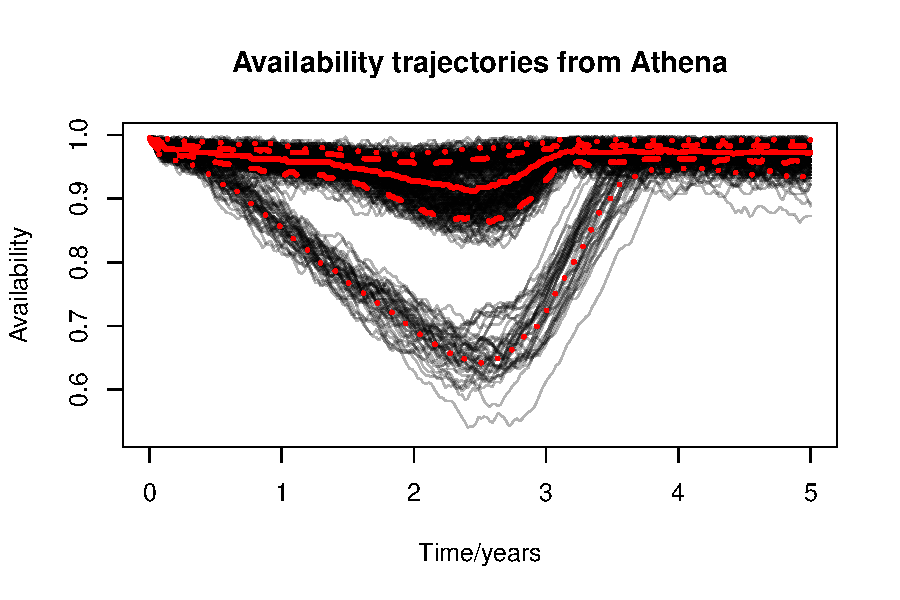
\includegraphics{fig-background/trajectories.pdf}
	\caption{A collection of $300$ typical availability trajectories (black lines) over the first $5$ years of a wind farm's operational life for a fixed set of parameter values. The solid red line represents the point-wise median trajectory, the dashed red lines represent $20^{th}$ and $80^{th}$  point-wise percentiles and the dotted red lines represent $5^{th}$ and $95^{th}$ point-wise percentiles.}
	\label{Fig:availability-trajectories}
\end{figure}
 In the first $5$ years of operation, \textit{excessive failure} is frequently observed. That is, the wind farm typically under-performs due to higher than expected numbers of component failures; tackling this issue is vital to the feasibility of offshore wind.

\subsection{A variant for spare components \label{Sec:athena-variant}}

The above description of the Athena simulator assumes that, when a subassembly suffers a failure that warrants replacement, rather than repair, that a replacement component is immediately available. In practice, this is an unrealistic assumption. Improving upon this assumption is necessary for our analysis in \cref{Ch:ds-for-ow}. A minor contribution of this thesis is some additional modelling within Athena to incorporate spare components and implementing this as simulator code.

A practical workaround to the problem of subassemblies being difficult to obtain, is to pre-order spare subassemblies and store them in a warehouse that is onshore, but close to the offshore wind farm. Within the Athena simulator, a subassembly can experience one of three types of failure. These are minor, moderate and severe failures. We have assumed that minor and moderate failures are of a nature such that they can be repaired with readily available tools or components. Severe failures are such that replacement of the subassembly is the only feasible option. We assume spare components are stored in a warehouse, which holds a fixed number of spare parts. At the start of the simulation, the user must choose how many of each spare part the warehouse can hold. These numbers are fixed for the entire simulation period. Denote the maximum number of spare subassemblies of type $i$ by $s_i$. Now let $s_i(t)$ be the number of spare parts we have available of type $i$ at time $t$. In essence, we have a finite number of spare parts readily available, which may be replenished at some future time.

Now suppose that a subassembly of type $i$ has suffered a serious failure. If there is a readily available spare part, then the part is shipped out to the turbine and it is repaired according to the processes within the `standard' version of the Athena simulator (so we still need the correct type of boat to be available, for example). If no spare part is available, because all the spares of type $i$ have been used, then the repair cannot take place until a new batch of spare parts arrives. This motivates a mechanism for ordering in more spare parts. We define a threshold, $s'_i$ such that, as soon as $s_i(t) < s'_i$, an operator within the wind farm places an order for more spare components. The $s'_i$ are specified at the start of the simulation and remain fixed for a given run of the simulator. The waiting time for the order is uncertain. If the order is placed at time $t$ then the order arrives at time $t + \Delta t$ where $\Delta t \sim Gamma(w_1, w_2)$, where $w_1$ and $w_2$ are uncertain parameters which could be elicited or specified by an expert.

There is also an extra mechanism regarding spare parts. It may be the case that the supplier cannot fulfil the order, or the order is only partially completed. We model the number of ordered spares that can actually be delivered, $s$, by a Binomial distribution; $s \sim Binomial(s_i - s_i(t), p)$. We would imagine that commonly, the order would be completely fulfilled. In such a case we can choose $p$ to be quite large, for example, $p = 0.99$. Whether an order can be fulfilled or not follows a Bernoulli distribution. We introduce a random variable $\omega \sim Bernoulli(p')$ where $p'$ is the probability that an order is fulfilled. $p'$ would typically take a large value, such as $0.99$. The total number of spares delivered from the order is then $s\omega$, and this is delivered at time $t + \Delta t$.

This concludes our introduction to the Athena simulator. We have introduced the necessary details for the applications later in this thesis, although more details can be found at \citet{Zit13, Zit16, Zit2021}.

\section{Elicitation of probability distributions \label{sec:prob}}

When quantities are unknown, and there is a lack of relevant data to estimate them, a feasible solution is to elicit them from an expert, or group of experts. Elicitation is the act of turning the knowledge or beliefs an expert has about unknown quantities into a joint probability distribution.

The elicitation of uncertain inputs, although useful when there is a lack of relevant data (or necessary if we wish to perform a Bayesian analysis utilising genuine prior beliefs), is a time consuming task which needs to be done carefully.

\subsection{The basics of elicitation}
In the elicitation process there are two roles. First we have the \textit{expert}. This is the individual whose knowledge or beliefs we aim to elicit and represent via a probability distribution. The term `expert' refers to their domain knowledge and expertise and has no reflection of their knowledge of statistics or probability. Commonly we will refer to multiple experts rather than singular; it is encouraged to combine the beliefs of multiple experts into a single distribution. The second role is the \textit{facilitator}; this a person who has good knowledge of probability and statistics, they guide the expert through the elicitation process and fit distributions to the elicited quantities.

Elicitation of a single uncertain quantity, $\theta$, is described as a four stage approach by \citet{Garthwaite05}.

The first stage is setting up the elicitation; this involves identifying an expert (or even a group of experts, as in \citet{Williams2021}), providing the experts with training and identifying precisely what $\theta$ is. By precisely, we mean that if $\theta$ is the rate at which the a gearbox, of brand X and model Y, would degrade at an offshore wind farm at location Z, then the experts should be told that $\theta$ is this value, rather than just ``the rate at which a gearbox degrades''.

The second task in the process is the `main' elicitation step: the expert states various summaries about $\theta$. Summaries are typically of the form $\p (a_i < \theta < b_i) = p_i$, $i = 1, 2, \ldots, n$. The facilitator can then fit a statistical model to the elicited $(a_i, b_i, p_i)$. In some cases we might be able to do this exactly and analytically. For example, if we elicit two quantities and assume $\theta \sim \mathcal{N}(\mu, \sigma^2)$, we can find $\mu$ and $\sigma$ via a pair of linear simultaneous equations in $\mu$ and $\sigma$. More generally, if there are more $p_i$ than parameters of the chosen distribution, or the form of the distribution does not lend itself to a tractable solution, then a numerical approach, \correction{such as minimising $T(\varphi) = \sum_i (p_i - \p (a_i < \theta < b_i \mid \bm{\varphi}))^2$ may be appropriate, where $\bm{\varphi}$ are the parameters of the distribution to be fitted.} This stage, and the previous stage, of fitting are somewhat interrelated; the form of the distribution the facilitator may wish to fit to the expert's beliefs may influence the questions asked. For example, when eliciting a distribution for a proportion, a Beta distribution, $\theta \sim Beta(\alpha, \beta)$, offers an appropriate model. Knowing that we will fit a Beta distribution to the elicited information means we would never ask the expert for $p_i$ such that $p_i = \p (5 < \theta < 50)$.

The `final' stage is then checking the adequacy of the fitted distribution. In this stage, the facilitator may show the expert what their elicited statements imply about $\theta$. If these statements are inconsistent with the expert's beliefs, we must go back and forth between the second, third and fourth stages until the expert and facilitator agree on a distribution, $\pi(\theta)$, which is an appropriate description of the expert's beliefs.

We have excluded the details about what kinds of questions a facilitator should ask the expert in order to obtain summaries of $\theta$. For guidance on the exact phrasing of questions, see \citet{Ohagan06}, in particular, Chapter $5$. Note that the types of questions to be asked are often related to the nature of the uncertain quantities, thus the general recipe for elicitation is necessarily vague. Some further practical guidance is given in \citet{Kadane1998}, who advocate for eliciting \textit{observable} quantities rather than the parameters of any statistical model. An observable quantity is, as its name suggests, a quantity that can be observed by the expert. This means we should ask experts about the quantities exhibited by a physical system (for example, a time to failure of a component in the wind farm), rather than parameters of a statistical model (for example, the parameters of a Weibull distribution).

\subsection{The Sheffield Elicitation Framework}
A popular elicitation procedure, the Sheffield Elicitation Framework (SHELF), provides a thoughtful routine for eliciting an unknown quantity from one or more experts. The procedure can be applied to a single expert, but we adopt the convention of multiple experts. SHELF is also used for multiple uncertain quantities, which we describe later.

SHELF consists of a collection of documents, which includes forms and presentation slides \citep{SHELF4}, this is accompanied by software to fit distributions to elicited beliefs, as well as validate them \citep{SHELFpkg}. Both the software and documents are designed to help the facilitator and the experts elicit an uncertain quantity of interest. SHELF covers all aspects of the elicitation process, from the recruitment of experts, to the `main' elicitation step, as well as checking the adequacy of $\pi(\theta)$ as a representation of the expert's knowledge of $\theta$. An important concept in SHELF is RIO: the rational impartial observer. RIO is a hypothetical fly on the wall who, if they had no strong beliefs about $\theta$ prior to observing the discussion amongst experts, would hold beliefs characterised by $\pi(\theta)$ after observing their discussion. The experts are instructed to formulate a distribution, $\pi(\theta)$, which summarises the knowledge of all the experts. This combined judgement does not have to be an equal weighting of each individual's beliefs; the experts are free to give more consideration to more knowledgeable experts as they see fit.
The core elicitation step is broken into two main parts; individual elicitation and a group elicitation as follows:\footnote{We have condensed the steps considerably. We aim to communicate the core steps in SHELF rather than replicate the documentation.}
\begin{itemize}
\item[1.] {Conduct an individual elicitation for each expert as follows:}
  \begin{itemize}
    \item[(i)] Specify a lower value, $L$, such that the event $\theta < L$ is `extremely unlikely'. By `extremely unlikely', it is meant that if you were to learn that $\theta < L$, your initial reaction would be that the statement $\theta < L$ is false. Repeat the process for an upper limit, $U$, where the event $U>\theta$ is extremely unlikely.
    \item[(ii)] Elicit the median, $m$ such that $p(\theta < m) = 0.5$. $m$ is the value that placing a bet on $\theta < m$ has an equally desirable outcome to placing a bet on $\theta \geq m$.
    \item[(iii)] Elicit a lower quartile, $Q_1$ such that $\p(L \leq \theta < Q_1) = \p(Q_1 \leq \theta < m) = 0.25$. As above, placing a bet on the event $L \leq \theta < Q_1$ should be equally desirable to placing a bet on the event $Q_1 \leq \theta < m$.
    \item[(iv)] Elicit an upper quartile, $Q_3$ such that $\p(m \leq \theta < Q_3) = \p(Q_3 \leq \theta < U) = 0.25$. This step is similar (iii).
    \item[(v)] The facilitator now fits a distribution to the elicited knowledge, treating the limits, quartiles and median as data.
  \end{itemize}
\item[2.] {Conduct a group elicitation as follows:}
  \begin{itemize}
    \item[(i)] As a group, perform all the steps in part 1.
    \item[(ii)] Verification: is the fitted distribution what a RIO would conclude as appropriate?
  \end{itemize}
\end{itemize}
This process is what we will describe as a `full SHELF' elicitation. Step $1. (v)$ can be performed in a semi-automatic way via the \texttt{SHELF::elicit()} function, which opens a Shiny app. The facilitator fills out boxes within the app corresponding to elicited information. The app can either fit a single chosen parametric form, or try many parametric forms and return the form which offers the closest fit to the elicited beliefs. A screenshot of the app is given  in \cref{Fig:shelf-app}. In the example, the elicited information leads to $\log \theta \sim t_{10}(6.02, 0.5)$, where $\theta$ is the number of coffees consumed in the production of this thesis and $t_\nu (\mu, \lambda^2) = \mu + \lambda t_\nu$ is a location-scale variant of the $t$ distribution.
\begin{figure}
  \centering
  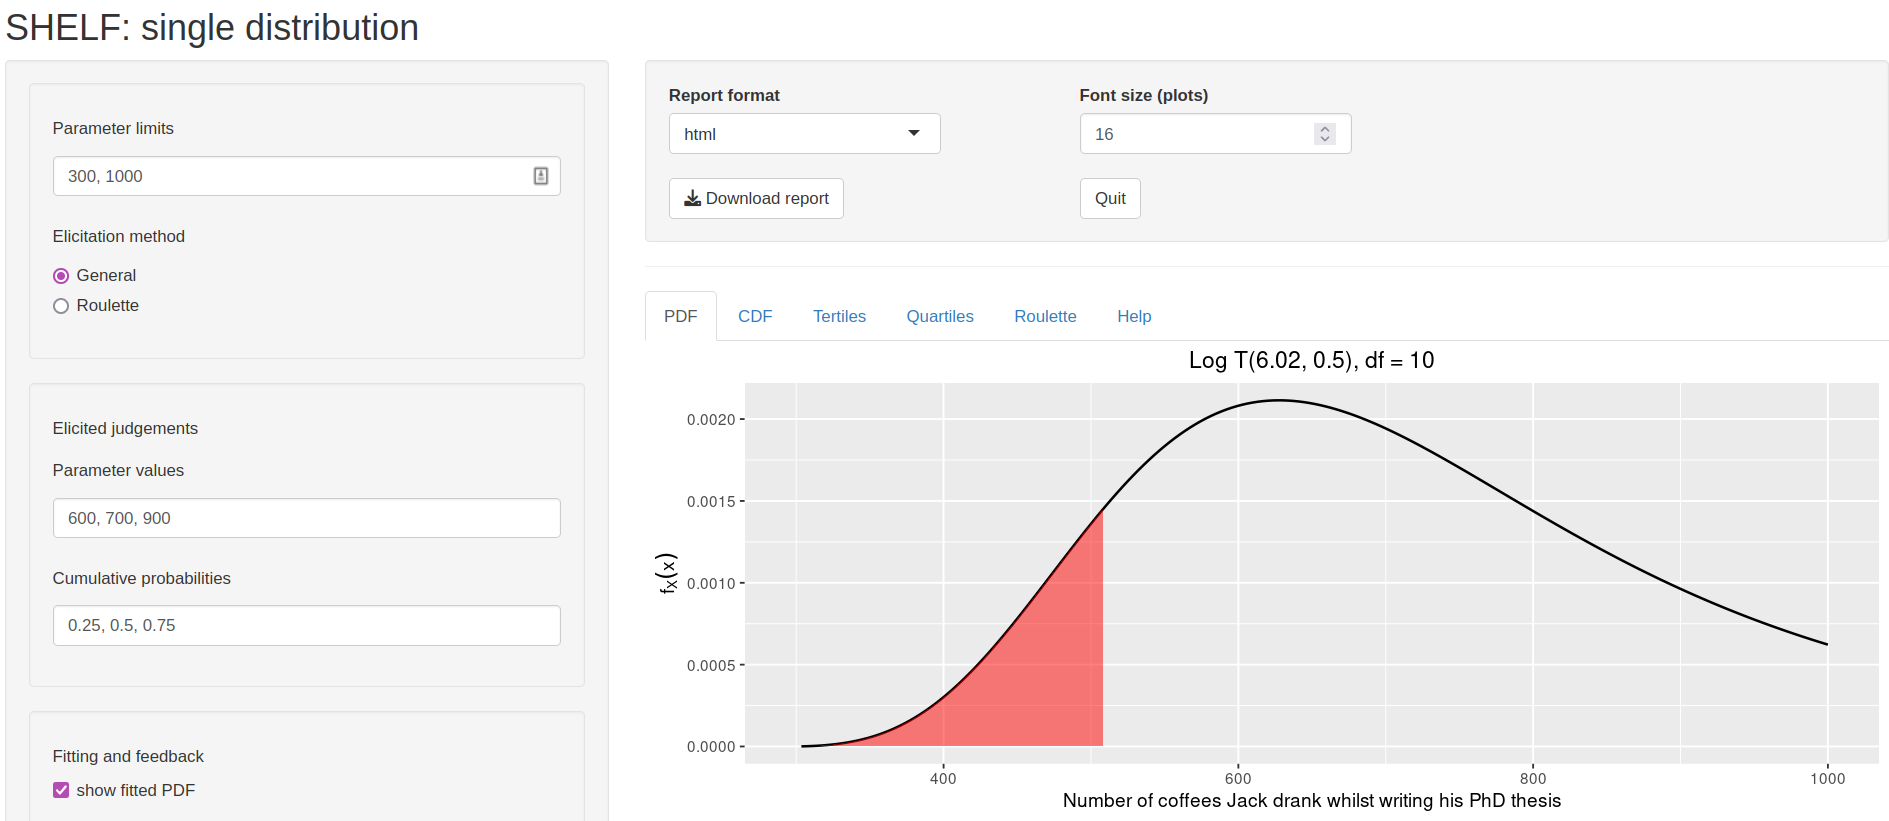
\includegraphics[width=\textwidth]{fig-background/shiny.png}
  \caption{Screenshot of distribution fitting functionality provided by the \texttt{SHELF} package \citep{SHELFpkg}. In this particular example, we have elicited the number of cups of coffee the author of this thesis believes he has drunk in order to complete this thesis. The red shaded area represents a feedback question.\label{Fig:shelf-app}}
\end{figure}
\subsection{Elicitation of many uncertain quantities}

Suppose we have $k>1$ uncertain quantities, $\btheta = (\theta_1, \theta_2, \ldots, \theta_k)^T$. We wish to characterise uncertainty about $\btheta$ via $\pi(\btheta)$, a joint density. If the expert is willing to assert that $\theta_i \indep \theta_j \,\forall\, i \neq j$, then we may write $\pi(\btheta) = \prod_{i=1}^k \pi_i (\theta_i)$. In this case, all we need to do is elicit $\pi_i(\theta_i)$ using the univariate method outlined above.

If the components of $\btheta$ cannot be assumed to be independent there are two approaches within SHELF. The first is to rephrase the problem in terms of new unknowns, $\btheta'$, such that $\theta'_i \indep \theta'_j \,\forall\, i \neq j$. For example, suppose we are planning the programme for a statistics conference, we may want to elicit
\begin{itemize}
  \item[(i)] $\theta_1 = \text{the number of delegates at a particular statistics conference}$
  \item[(ii)] $\theta_2 = \text{the number of delegates at the conference who are Bayesian}$.
\end{itemize}
Clearly, $\theta_1 \geq \theta_2$, thus a dependence is present. Now let $\theta'_1 = \theta_1$ and $\theta'_2 = \theta_2/\theta_1$, that is, the proportion who are Bayesian. The statement $\theta_1' \indep \theta_2'$ seems more plausible than $\theta_1 \indep \theta_2$. We recover $\btheta$ via $(\theta_1, \theta_2)  = (\theta'_1, \theta'_1 \theta'_2)$.

The second approach is to try to elicit the dependence between elements of $\btheta$. This is a much more challenging task than assuming independence, thus should only be done when necessary. Within SHELF, dependence may be elicited via assuming an appropriate distributional family that lends itself well to dependence (for example, multivariate Normal or Dirichlet). The second option is to incorporate dependence via a copula. A copula is a useful device for constructing a dependence structure between two random variables with known marginal distributions \citep{Bedford2014, Elfadaly2017}. In either case, we must elicit marginal distributions and the dependence structure.

Eliciting even the marginal distributions can take a long time. The European Food Safety Authority (EFSA) state that elicitation of a single unknown takes about a day \citep{EFSA2014}. EFSA believe that elicitation of $4$--$6$ parameters takes about $2$ days. The experts are able to perform elicitation more quickly because they become accustomed to the process. Elicitation workshops are time limited for practical reasons. The first is that experts will become fatigued, thus after several days their judgements degrade in quality. The second is that experts will only be available for a limited amount of time; they will have other commitments. We may only have access to the experts for a day or so. For this reason, we must think carefully about which parameters deserve a full SHELF treatment and which parameters require less thought. This amounts to different types of elicitation. The most rigorous is the full SHELF treatment, reserved for the most important parameters.

An approach that is less involved than SHELF, but retains many of its features is probabalistic Delphi \citep{Rowe1999}, which can take place remotely (for example, via email).  A questionnaire about unknowns, with questions similar to that found in a full SHELF workshop, is sent to experts, which they return to the facilitator. The questionnaire responses are then circulated anonymously amongst all experts so they can review the other opinions about $\btheta$ and revise their own beliefs as appropriate. The revised beliefs are sent to the facilitator who then uses a mathematical aggregation rule --- such as a linear combination of each expert's $\pi(\btheta)$ --- to combine each expert opinion into a single distribution.

A less sophisticated, but much less time consuming, approach would be to employ a `minimal assessment'. Minimal assessment may proceed by eliciting $L$ and $U$ from each expert, then for the facilitator to assume a very simple form for $\pi_i(\theta_i)$. For example, we might take $\theta_i \sim \mathcal{U}(L, U)$. Another simple form would be $\theta_i \sim \mathcal{N}(\mu, \sigma^2)$  with $\mu = \frac{1}{2}(L+U)$ and $\sigma = \frac{1}{2}(U-\mu)$ (remembering that $95\%$ of a Normal distribution's mass lies within $\pm 2 \sigma$  of  $\mu$). Each expert's $L$ and $U$ could be revised via a Delphi-like approach, or the facilitator could take $L^{*} = \min{L}$, $U^{*} = \max{U}$ and fit a distribution based on $U^{*}$ and $L^{*}$. A minimal assessment is often employed when we want to use expert judgement for a prior in a Bayesian analysis, but we know that a reasonably large sample of data is available. The sample will be sufficiently large to dominate any prior specification, thus we choose not to worry about precise details of $\pi(\btheta)$.

How we choose which parameters warrant a full SHELF treatment and which parameters require a less formal treatment can be dealt with via a sensitivity analysis. In almost all cases, the distribution $\pi(\btheta)$ is not of direct interest. We are usually interested in the distribution $\pi(\btheta)$ induces on $f(\btheta)$, a function of the uncertain parameters. Concretely, we may want to propagate uncertainty about model parameters, $\btheta$ through a complex model (such as the Athena simulator) to make predictions about quantities relevant to decision making, such as the availability time series,  or summaries of it. The SHELF documentation suggests that a one-way sensitivity analysis may be appropriate. In this case we study how much $f(\btheta)$ changes when $\theta_i$ is perturbed to $\theta_i \pm \Delta \theta_i$. How much $f(\btheta)$ changes when only $\theta_i$ changes is a simple, but limited, way to investigate the relative importance of each $\theta_i$. In \cref{Ch:sensitivity} we give an in-depth discussion of sensitivity analysis, the relative importance of parameters, and best practices for sensitivity analysis with a view towards eliciting uncertain parameters of a model.

\section{Decision analysis \label{sec:decision}}

Unless explicitly stated otherwise, this section is based upon \citet{Keeney1976}, \citet{Smith2010} and chapters of \citet{ElicitationBook}; in particular \citet{Gonzalez2018}.

In many of the decision making situations we encounter in our lives, our idea of the `best' decision may differ to another person's idea about what is the `best' decision. Consider the problem of preparing a scone to be eaten. One individual may claim that putting jam on a scone \textit{before} the cream is objectively the best method to prepare it. Many other people would express dogmatically that the cream \textit{must} be first. Others would argue that the best way is not defined by the ordering of cream or jam, but much rather, the quantity of cream and jam.

These differences are present because every decision maker (DM) has their own preferences. Much like how we all have different prior beliefs for an unknown quantity, we also have different preferences for outcomes and thus different optimal decisions. A DM's preferences are expressed via a utility function which can be elicited from the DM. This function can have different shapes for different DMs. In fact, different DMs may have utility functions which have different inputs. We will now formalise the notion of a utility function.

Let $\calX$ represent the set of all possible decisions the DM could make, and let $\bx \in \calX$ be a single decision. Further suppose that any relevant unknown quantities, $\btheta$, within the decision problem have been assigned a probability distribution $\btheta \sim \pi (\btheta)$. In this thesis $\pi(\btheta)$ will usually be an elicited prior distribution, but it should be replaced by the posterior distribution $\pi(\btheta \mid \by)$ when relevant data $\by$ are available. Finally, we need a function $u(c(\bx, \bphi))$ which is a mathematical representation of the DM's beliefs for how desirable the consequence $c(\cdot, \cdot)$ is when decision $\bx$ has been made and when $\btheta$ takes the value $\bphi$. The function $c(\cdot, \cdot)$ may be deterministic when it is clear how decisions impact future events, or it can be a stochastic function when future events are uncertain.

The optimal decision is given by
\begin{equation}
  \bx^{*} = \argmax_{\bx \in \calX} U(\bx). \label{Eq:opt-dec}
\end{equation}
where
\begin{equation}
U(\bx) = \E_{\btheta} \{ u(c(\bx, \btheta)) \} \label{Eq:exp-util}
\end{equation}
is the expected utility of the decision $\bx$. The expectation in \cref{Eq:exp-util} depends on several things:
\begin{itemize}
  \item[(i)] $\pi(\btheta)$, the probability distribution over all relevant unknown quantities
  \item[(ii)] $c(\bx, \btheta)$, the \textit{consequence} of decision $\bx$ when the unknown quantities take the value $\btheta$.
  \item[(ii)] $u(c(\cdot, \cdot))$, the utility function describing how preferable a consequence is. Larger values of $u(c(\cdot, \cdot))$ indicate more preferable consequences.
\end{itemize}

For many problems, an `off the shelf' utility function may adequately describe our preferences. For example, in Bayesian design of experiments, the goal is often to choose a design $\bx \in \calX$ which allows us to learn the most about some unknown quantities. One appropriate, default utility function is the Kullback-Leibler divergence between the prior and posterior distributions for the unknowns. A review of appropriate utility functions for Bayesian design of experiments is given in \citet{Ryan2016}.

For many practical problems, there are many competing objectives which may not be well defined. For example, we would typically want to maximise energy output of the wind farm, and simultaneously minimise operation and maintenance costs. These objectives compete with each other. Increasing maintenance costs may increase energy generation, for example. A less well defined objective is keeping local residents happy with the development of the offshore wind farm, in such a case we must come up with a \textit{proxy} for resident discontent which we can observe. The DM may wish to re-phrase resident discontent as the number of local residents who sign a petition against the development of an offshore wind farm, for example.

Since the development of an offshore wind farm is a highly specialised problem, it is unlikely that an off the shelf utility function will describe the objectives we wish to achieve. Further, different decision makers may have different preferences. For example, the CEO of an energy company may be mainly motivated by profits, whereas, a systems safety engineer's first priority is the safety of those maintaining the wind farm. Therefore, once a DM has been chosen, we need to encode their unique preferences into a utility function. This is done by \textit{eliciting} the utility function, $u(\cdot)$ from the DM. We must also elicit $\pi(\btheta)$. We do this via the methods given in \cref{sec:prob}.

We now provide an overview of some utility elicitation techniques. This allows us to turn an ill-defined decision problem into the well-posed questions of mathematical optimisation.

\subsection{Fundamental notions of utility}

There are three axioms of utility theory under risk, where a preference relation $\preceq$ is assumed on a probability space $\mathcal{P}$. To discuss the fundamental notions of utility we need to define a \textit{lottery}. A lottery, $p = [x, y; r]$ is an uncertain event where $p = x$ with probability $r$ and $p = y$ with probability $1-r$. For lotteries $p$ and $q$ the statement $p \preceq q$ means that $q$ is \textit{at least} as desirable as $p$. \correction{The statement $p \prec q$ means that $q$ is more desirable than $p$.}

The three axioms are as follows:
\begin{enumerate}
\item \textbf{Weak order:} $\preceq$ on $\mathcal{P}$ is complete; $\forall$ $p, q \in \mathcal{P}$ either $p \preceq q$ or $q \preceq p$ and is transitive; $\forall p, q, r \in \mathcal{P}$  $p \preceq q$ together with $q \preceq r$ $\implies$ $p \preceq r$.

\item \textbf{Archimedian:} $\forall p, q, r \in \mathcal{P}$ if $p \prec q \prec r$ then $\exists \alpha, \beta \in (0, 1) $ such that $\alpha p + (1-\alpha)r \prec q \prec \beta p + (1-\beta) r$.

\item \textbf{Independence:} $\forall p, q, r \in \mathcal{P}$ and $\alpha \in (0, 1]$, $\alpha p + (1-\alpha)r \preceq \alpha q + (1-\alpha) r \iff p \preceq q$.
\end{enumerate}
Under these conditions there is a \textit{utility function}, $u$, satisfying $\forall p, q \in \mathcal{P}$
\begin{enumerate}
\item[(i)] $p \preceq q \iff u(p) \leq u(q)$
\item[(ii)] $u(\alpha p + (1-\alpha) q) = \alpha u(p) + (1- \alpha)u(q)$.
\end{enumerate}
From this, we can deduce $p \preceq q \iff \E_p(u) \leq \E_q(u)$, where $\E_p(u)$ is the expected utility of a lottery $p$.

Note that a utility function is only unique up to a positive affine transformation; $au(\cdot) + b$, for any $a >0$ and $b \in \mathbb{R}$, represents the same set of preferences as $u(\cdot)$.

\section{A basic single attribute utility elicitation}

One of the first steps in a decision analysis is to decide what we measure to decide how good a decision is. The attribute is the quantity that we measure to describe how preferable a decision is. Common attributes would be financial gain in a business setting or whether an individual recovers from surgery in a medical setting. The consequence is the realised value of an attribute after making a decision.

When eliciting a utility function for an uncertain consequence, $c(\cdot, \cdot)$, it is much easier to consider trade-offs under certainty. We therefore elicit the utility function as a function of consequences $c$ rather than decisions $\bx$ and unknown states $\btheta$. When finding the optimal decision, we revert to consequences being uncertain; that is, replace $c$ by $c(\bx, \btheta)$. We then calculate $\bx^{*}$ by optimising $U(\bx)$ (\cref{Eq:exp-util}) with respect to the decision, $\bx$.

A basic elicitation procedure is as follows. We assume that $u(c)$ is monotonically increasing in $c$.

\begin{enumerate}
	\item Determine $[c^0, c^*]$; the range for the attribute of interest. Assume $c^{0} \prec c^{*}$.
	\item Set $u(c^*) = 1 - u(c^0) = 1$.
	\item Elicit utilities $\{u_1, \ldots, u_n\}$ for a set of intermediate consequences $\{c_1, \ldots, c_n \}$.
	\item Fit a utility function to the quantities $\{(c^0, 0), (c_1, u_1), \ldots, (c_n, u_n), (c^*, 1) \}$. This can be done via a least squares procedure.
	\item Check for consistency; ask  the DM a few verification questions.
\end{enumerate}
The above recipe assumes a given functional form for $u(\cdot)$; choosing this functional form can be tricky. Further, assigning utility values to intermediate values is not trivial. It is also important to be aware of, and counter, the DM's inaccuracies and biases. If $u(c)$ is not monotonically increasing in $c$, the problem can frequently be rephrased so that $u(c)$ is monotonically increasing in $c$. For example, replacing $c$ by $-c$ when $u(c)$ is monotonically decreasing, or replacing $c$ by $(c - c')^2$ if $u(c)$ is increasing on $[c^{0}, c']$ then decreasing on $(c', c^{*} ]$.

The main step in the above procedure is step $3$: eliciting utilities for intermediate consequences. The number $n$ of utilities to be elicited will be a trade off between the accuracy of the resulting utility function and the time available.

There are two main ways to elicit $u_i$ in step $3$. The first is \textit{probability equivalence}. Here the DM must specify the probability $p$ where $[c^{*}, c^{0}; p] \sim c$ for a pre-determined consequence $c$. The notation $[c', c''; p] \sim c$ describes a lottery where $c'$ occurs with probability $p$, $c''$ occurs with probability $1-p$, and the uncertain result of this lottery is as desirable as the certain consequence $c$; that is $U([c', c''; p]) = U(c)$. The other way is to specify one of $\{ c, c', c''\}$ when $p$ and the other two elements of $\{c, c', c'' \}$ are determined. This is a \textit{certainty equivalence}.

Within each of the two main elicitation approaches, there are choices about how to specify probabilities and consequences. This concerns the choices of the multiple $c_i$ in the $(c_i, u_i)$ pair, or choosing related values of $p$ when constructing many certainty equivalences. Each of these has limitations, which are typically forms of biases, as well as advantages; see Section $10.2.2$ and Section $10.2.4$ of \citet{Gonzalez2018}, as well as references within for a discussion of the various biases that can occur when eliciting utilities and how to counteract them.
\subsection{Multi-attribute utility elicitation}
When eliciting a multi-attribute utility function (where the consequence space has $2$ or more dimensions), it is cognitively complex for the decision maker to simultaneously weigh up the relative merits of many consequences. For this reason, much like probability elicitation, the problem can be greatly simplified when certain notions of independence are assumed. The notion of independence we need is known as \textit{preferential independence}. Two (collections of) attributes $\mathcal{C}_i$ and $\mathcal{C}_j$, with $\mathcal{C}_i \cap \mathcal{C}_j =\emptyset$ are said to possess preferential independence if
\begin{equation*}
  (c_i, c_j) \succeq (c_i', c_j) \implies (c_i, c'_j) \succeq (c_i', c_j')
\end{equation*}
for some $c_j$ and all $c_j'$. \correction{We have introduced the symbol $\succeq$ which is similar to $\preceq$: $p \succeq q \iff q \preceq p$.} This type of independence allows the DM to specify judgements of the form \textit{``provided everything else is constant, I prefer X to Y''}. This allows us to elicit individual utility functions for each attribute $\mathcal{C}_i$ and then combine them to provide an `overall' utility function for all $m$ consequences, $\mathcal{C} = \mathcal{C}_1 \times \mathcal{C}_2 \times \ldots \times \mathcal{C}_m$. If preferential independence holds for all possible sets $i$ and $j$ then the DM views the consequences as \textit{mutually preferentially independent}. This is sometimes referred to as having \textit{mutually utility independent} consequences.
Now, assuming that consequences are mutually utility independent, there are two main ways to proceed. The first is to elicit a utility function which is a weighted sum of the marginal utility functions:
\begin{equation}
  u(c) = \sum_{i=1}^m w_i u_i(c_i). \label{Eq:add-util}
\end{equation}
This is appropriate when the DM's preferences between lotteries depends only on the marginal distributions over the $\mathcal{C}_i$ and not their joint distribution. If preferences depend on the joint distribution, then we should use a multiplicative form:
\begin{align}
  u(c) &= \sum_{i=1}^m w_i u_i(c_i)\label{Eq:mult-util}\\
        &+ k\sum_{i=1, j>i}^m w_iw_j u_i(c_i) u_j(c_j) \nonumber\\
        &+ \ldots  \nonumber\\
        &+ k^{m-1}w_1 w_2 \ldots w_m u_1(c_1) u_2(c_2)\ldots  u_m(c_m) \nonumber
\end{align}
where $w_i$ are weights to be elicited and $1 + k = \prod (1 + k w_i)$. The case $k = 0$ corresponds to the additive utility function in \cref{Eq:add-util}.

In the case of \cref{Eq:add-util} we can elicit the weights, $w_i$, by considering the consequence $c_{(i)}^0 = (c_1^0, c_2^0, \ldots, c_{i-1}^0, c_i^{*}, c_{i+1}^0, \ldots, c_m^0)$. $c_{(i)}^0$ is the consequence where all attributes are at their worst value, apart from the $i$th attribute which is at its best value. It is simple to verify that $u(c_{(i)}^0) = w_i$. This gives rise to an elicitation protocol where we cycle over the $c_{(i)}^0$ to obtain each $w_i$. Note that $\sum_{i=1}^m w_i = 1$ since the best consequence, $c^{*}$, satisfies $u(c^{*})=1$, and the worst consequence, $c^0$, satisfies $u(c^0) = 0$. This means only $m-1$ statements are required to elicit the $w_i$; additional statements can be used for verification. If the multiplicative form is used, one extra question needs to be asked. For example, we could invert one of the $c_{(i)}^0$ and have all but the $i$th consequence at its best value, and have the $i$th consequence at its worst value.

\subsection{Choosing functional forms for the $u_i$}

One of the most important issues is choosing the \textit{functional form} of the utility function. Two important features are: monotonicity (more profit is almost always preferred) and concavity (an assumption about the attitude to risk of the DM).

Suppose $C \in \mathbb{R}$ is a monetary consequence. For a lottery $p$ there are two expectations to consider. The \textit{expected utility} $\E_p[u(c)]$ and the expected (monetary) value $\E_{p} (c)$. The certainty equivalent, $c_p$ is the amount of money the DM would place on a single play of the lottery; $u(c_p) = \E_p(u(c))$. Equivalently, $c_p = u^{-1} \left\{ \E_{p} (u(c)) \right\}$.

The risk premium is defined to be the difference between the expected value of the lottery, and its certainty equivalent. We can interpret this as the difference in the value of infinite plays of the lottery versus a single play:

\begin{equation}
	\pi_p = \E_p (c) - c_p.
\end{equation}

The sign of $\pi_p$ is a result of the shape of $u$. $u$ is concave $\iff$ $\pi_p > 0$;  in such a scenario the DM is described as `risk averse'. An alternative phrasing of a risk averse attitude is preferring the average result from many plays of the lottery, to a single play of the lottery. A risk averse DM prefers a small deterministic payoff to a random payoff with larger expected value, but some chance of a very small payoff. This is common in financial situations. A risk prone DM ($\pi_p < 0$) will prefer the lottery to its expected consequence; a desperate individual may wish to spend their last $\pounds 1$ on a scratch card, since the prospect of winning thousands is much more appealing than the fact that they will probably lose their stake.

Of course, a decision maker does not have to be strictly risk prone or strictly risk averse. They could be risk neutral (in this case $u(x) = ax + b$ and $\pi_p  = 0$) or they could have a varying attitude towards risk. For instance, suppose the DM is a student who is planning their revision strategy for a pass/fail exam. Suppose the pass mark is $60\%$. When considering their revision strategy, the DM is willing to do almost anything that will get them above the pass mark. However, the DM is not desperate to achieve very high marks (although a very high mark would bring an increased level of personal achievement, which does increase the DM's utility of such events). For events below the pass mark, the DM will be risk prone, for events above the pass mark the DM will be risk averse; this leads to a sigmoidal shape. This is an example of the \textit{local} risk behaviour changing.

Choosing the best functional form from many candidate functional forms can be achieved by considering, for example, the sum of squares in the least-squares procedure used to find the parameters for any given functional form. Verification questions can also be used to see which functional forms are, or are not, consistent with the preferences of the DM. For example, we could ask the DM  for $c'$  such that $u(c')  = u'$, where  $u'$ is not close to any of the previously elicited $u_i$. If $u'$ is close to the fitted $u(c')$ then we would be comfortable with the fitted $u(c)$. If it is too far away, we should consider alternative functional forms, or even re-elicit the $(c_i, u_i)$ pairs. We should also verify with the DM, once we have constructed and optimised $U(\bx)$, that $\bx^{*}$ is a decision they would be willing to take. If $\bx^{*}$ is not a decision that the DM is willing to take, this suggests that somewhere in the process there has been an error, or the DM has changed their preferences. In such cases, we must go back to the start and re-elicit all attributes and functional forms.

\section{Discussion}

We have outlined some relevant background material to set the scene for the rest of this thesis.

We have introduced the Athena simulator, a stochastic point-process model used to make statements about the reliability of an offshore wind farm, with a view towards making decisions about the operations and maintenance of the wind farm. The Athena simulator is typical of many simulators within the wider area of reliability analysis as it is stochastic, expensive and relies on many uncertain parameters. This makes the Athena simulator a suitable example for extensive case studies within later chapters.

We then discussed one approach that a subjective Bayesian may use to elicit a (joint) probability distribution. This approach is known as SHELF. We discussed that elicitation is useful when there is a lack of relevant data, although it is not a trivial procedure. We must take great care to elicit an honest and faithful representation of the beliefs experts possess. SHELF promotes the use of sensitivity analysis to gauge the relative importance of each element of $\btheta$, in order to obtain the most useful belief specification about $\btheta$ in the time available.

Finally, we introduced some basic concepts of decision making, such as utility, as well as motivating subjective utility functions as ways to capture the preferences of a DM and the trade-offs that they must make in complex problems. We discussed some approaches to eliciting multi-attribute utility functions by comparing a given lottery to certain consequences. We discussed ways to combine given marginal utility functions into a multi-attribute utility function. We also discussed aspects of choosing the functional form of the marginal utility functions.
\end{chapter}

  \begin{chapter}{Emulators \label{Ch:Emulators}}
Computer models, or simulators, allow us to predict complex phenomena at little financial or ethical cost. In a wind farm setting, it would cost an extortionate amount of money and literally years of time to test how a real, full scale wind farm performs under a single set of parameter values. Now suppose an engineer wants to know what would happen if we tweaked the set up in some way, corresponding to a change of simulator parameters. This is could be a multi-million pound question. Computer models allow us to investigate many ``what if'' scenarios at a fraction of the time and cost of the real thing. There are also ethical concerns that computer models may address; poor wind farm design is problematic for wildlife and endangering human life \citep{Bailey2014, Pedersen2020}. Athena does not address all of these concerns, but it certainly will get us a long way without costing us much money.

Although simulators such as Athena alleviate the financial and ethical burden associated to large scale physical experiments, they are often computationally costly. Most of the runs of Athena in this thesis take approximately $5$ minutes. This timing is somewhat variable since different experiments were performed on different machines, and certain parameter settings take longer to run than others. Most of the work in this thesis concerns exploring the parameter space to inform decision making. We require tools to reduce this computational cost. We will now step away from Athena, and its use cases, to consider how we can use statistical methods to build fast approximations to complex computer models as a general task. That is, construct \textit{emulators} for computer simulators.
\section{Gaussian process priors}
Formally, a Gaussian process (GP), is a stochastic processes such that any finite collection of variables from this process follows a multivariate Normal distribution. In this thesis, GPs are viewed as prior distributions for \textit{functions}. If we want to specify a GP prior, for a function $f(\cdot)$, then we only need to specify a mean function,
\begin{equation}
  \mu(\bx) = \E \{ f(\bx) \}
\end{equation} and a covariance function
 \begin{equation}
   C(\bx, \bx') = \cov\{ f(\bx), f(\bx')\}
 \end{equation}
where $\bx$ and $\bx'$ are inputs to the computer model. Usually $\bx$, $\bx' \in \R^k$ for some $k \geq 1$.

The purpose of the mean function is clear. $\mu(\bx)$ is a functional form and should provide a sensible global estimate for $f(\bx)$. What allows GPs to be more flexible than approaches such as linear models is the covariance function; \correction{covariance functions allow us to concisely specify complex structure such as highly nonlinear behaviour.} For now we will just set $\mu(\bx) = 0$ but we will return to more general forms for $\mu(\bx)$ soon.

\subsection{Covariance functions}
By definition, the covariance function describes the covariance between two function outputs. It is the covariance function that allows us to specify a prior over many possible functions, rather than just specific functional forms. Here we review some common covariance functions with an emphasis on the ones used in this thesis. For a longer discussion we direct the reader to \citet{Rasmussen2006Gpfm}.

In general, covariance functions can be written as
\begin{equation}
  C(\bx, \bx') = \sigma^2 r(\bx, \bx')
\end{equation}
where $\sigma^2$ is a scale parameter and $r(\cdot, \cdot) \in [-1,1]$ is a correlation function. The `meat' of the covariance function is $r(\cdot, \cdot)$; this is the device that allows us to specify the (prior) behaviour of uncertain functions. The role of $\sigma^2$ is to transform the correlation function from a unitless quantity to the same units (and scale) as $f(\bx)^2$. An important property of a correlation function is that it is a \textit{positive semidefinite function}. This means, for any $(w_1, w_2, \ldots, w_n) \in \R^n$, and vectors $\bx_1, \bx_2, \ldots, \bx_n \in \R^K$
\begin{equation}
  \sum_{i = 1}^n \sum_{j = 1}^n w_i w_j r(\bx_i, \bx_j) \geq 0.
\end{equation}
This property is closely related to the notion of a positive semidefinite matrix, which are used to form covariance and correlation matrices. In particular, if $r(\cdot, \cdot)$ is a positive semidefinite function, then a matrix $R$ with $R_{i,j}  = r(\bx_i, \bx_j)$ is a positive semidefinite matrix.

\correction{First we consider a squared exponential covariance function.} For a function $f(\cdot)$ with scalar input $x \in \R$, the squared exponential covariance function is given by
\begin{equation}
  C(x, x') = \sigma^2 \exp\left\{ -\frac{(x - x')^2}{\theta^2} \right\}.
\end{equation}
The scale parameter $\sigma^2$ corresponds to a prior marginal variance. If we take $\sigma = 1$ and model $f(\cdot)$ as a GP then we believe that around $95\%$ of function values lie in the range $(-2, 2)$. The covariance function is a scalar multiple of a correlation function. In the case of a squared exponential, the correlation function is $r(\bx, \bx') = \exp\left\{  -\frac{(x - x')^2}{\theta^2} \right\}$. The parameter $\theta$ is a \textit{lengthscale} parameter which describes how informative $f(x)$ is for $f(x')$ the (Euclidean) distance between inputs. Stationary covariance functions are those which depend only on \correction{$d(x, x') = |x - x'|$;} we can see that this holds for the squared exponential covariance function thus a GP with squared exponential covariance is a stationary process \citep{Gneiting2002}.

As \Cref{Fig:sqexp} shows, for small values of $\theta$ the correlation between inputs decays very quickly --- at an exponential rate. \correction{For larger $\theta$, the correlation still decays exponentially, but at a reduced rate}. Smaller $\theta$ values generate less ``wiggly'' functions. Several draws from a GP with $\theta = 0.1$, $0.5$, $1$ and $2$ can be seen in \Cref{Fig:random-funcs}. Once \correction{$|x - x'| > 2\theta$} the function outputs are essentially uncorrelated. We have fixed $\sigma = 1$ in \Cref{Fig:random-funcs}, changing $\sigma$ just changes the scale of the generated functions but not their behaviour.
\begin{figure}[h]
  \centering
  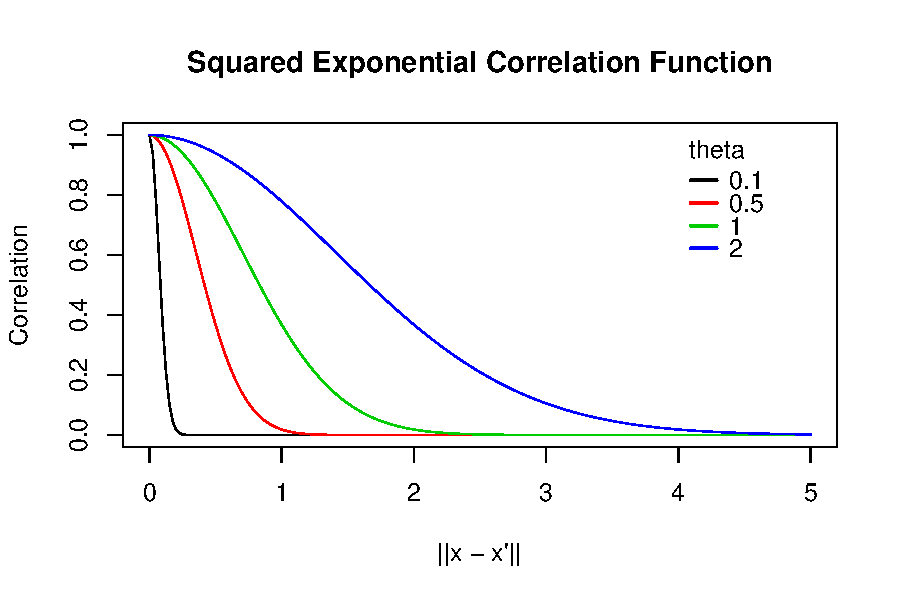
\includegraphics[width=\textwidth]{fig-emulators/squexp.pdf}
  \caption{Plot showing how $\theta$ affects the rate of decay of the correlation between model outputs as a function of the distance between inputs. Correlation functions with smaller values of $\theta$ decays to zero faster than those with a larger value of $\theta$.}
  \label{Fig:sqexp}
\end{figure}
\begin{figure}[h]
  \centering
  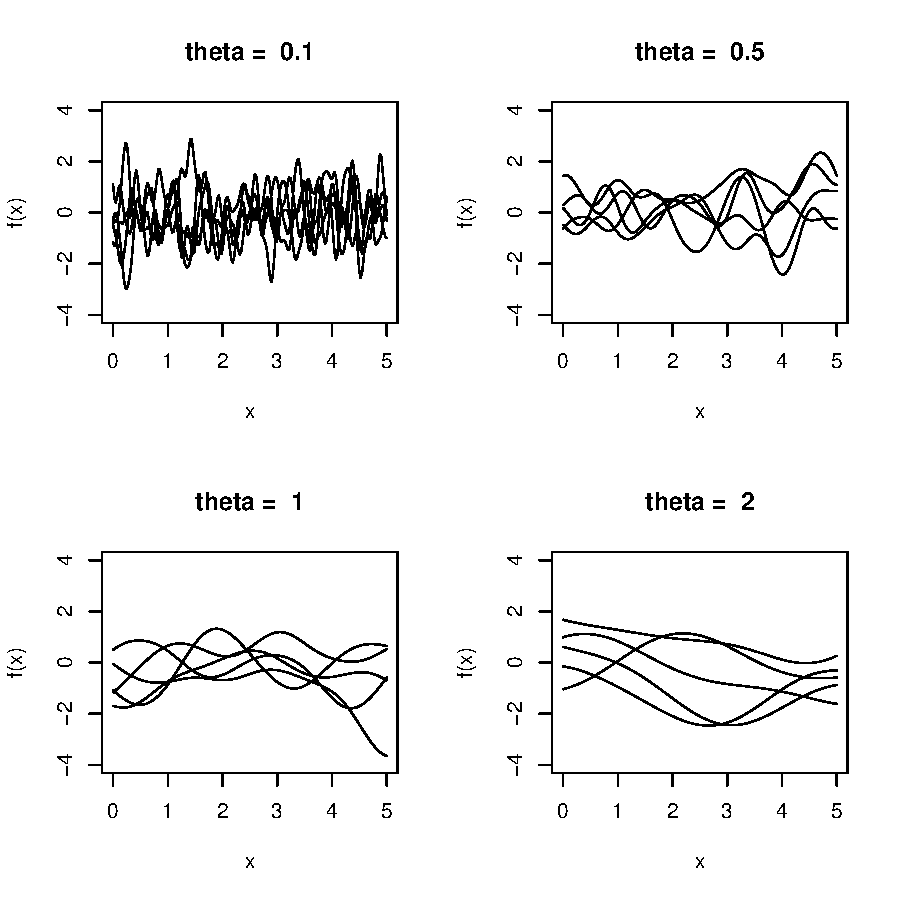
\includegraphics[width=\textwidth]{fig-emulators/random-func.pdf}
  \caption{Draws from a GP prior with squared exponential covariance function ($\sigma^2 = 1$) for varying values of $\theta$. Larger lengthscales correspond to less wiggly functions; their behaviour is less erratic.}
  \label{Fig:random-funcs}
\end{figure}
Note that, although small lengthscales lead to very wiggly functions, it can be shown that functions drawn from a GP with squared exponential covariance are infinitely mean square differentiable. This seems reasonable for the functions we will encounter later in this thesis. Note that, although each function is drawn randomly, each realisation from a GP represents a deterministic function. It is as if we were to randomly draw parameters of a fixed functional form. The precise form is unknown, but not inherently stochastic. These ``spaghetti plots'' are great for visualising \textit{joint} behaviour of function draws, but not very good at showing us the marginal behaviour. To do this, we can plot the prior mean and some chosen prior quantiles. In the case of a stationary covariance function, $C(x, x) = \sigma^2$ and because we assumed a zero mean GP the (prior) marginal behaviour is independent of $x$; $f(x) \sim  \mathcal{N}(0, \sigma^2)$.

The squared exponential is a limiting case of the Mat\'ern covariance function, which can be used to generate functions with a finite number of derivatives:
\begin{equation}
\correction{  C(x, x') = \sigma^2 \frac{2^{1-\nu}}{\Gamma(\nu)} \left( \sqrt{2\nu}\frac{|x - x'|}{\rho} \right)^\nu K_\nu\left(\sqrt{2\nu}\frac{|x - x'|}{\rho} \right)}
\end{equation}
where $\sigma$, $\rho$, $\nu > 0$ and $K_\nu$ is the modified Bessel function of the second kind. Functions drawn from this prior are differentiable $\lfloor \nu \rfloor$ times in the mean-square sense. Letting $\nu \to \infty$ recovers the squared exponential covariance function. Like the squared exponential covariance function, the Mat\'ern covariance function is a stationary covariance function.

Another common covariance function is the linear covariance function:
\begin{align}
  C(x, x') &= \begin{pmatrix}
    1&x
\end{pmatrix}
\begin{pmatrix}
  b_0 & b_1 \\
  b_1 & b_2
\end{pmatrix}
\begin{pmatrix}
  1 \\ x'
\end{pmatrix} \\ \nonumber
  &= b_{0} + b_{1}(x + x') + b_2 x x'.
\end{align}
The linear covariance function depends explicitly on $x$ and $x'$, and not the distance between them. This makes it a non-stationary covariance function. We later show that the linear covariance function is strongly related to many useful mean functions.

The final covariance function we consider is the white noise covariance function. This is just
\begin{equation}
  C(x, x') = \lambda^2 \mathbb{I}(x = x')
\end{equation}
where $\mathbb{I}(X)$ is an indicator function of the form
\begin{equation}
  \mathbb{I}(X) = \begin{cases}
    1, & X = \texttt{TRUE}\\
    0, & \text{ otherwise.}
  \end{cases}
\end{equation}
This covariance function is differentiable precisely \textit{nowhere}. It can be used to generate independent and identically distributed (iid) $\mathcal{N}(0, \lambda^2)$ random variables (RVs). It is not useful on its own for generating functions but does act as a useful device for modelling random variation exhibited by a stochastic simulator such as the Athena simulator.

In the context of emulation, $\lambda^2$, the variance of a random error term, is often called the `nugget' variance \citep{Gramacy12}. Throughout this thesis, we will use both $\sigma^2$ and $\lambda^2$ as variances of Normal distributions. Unless explicitly stated otherwise, $\sigma^2$ will be the marginal (prior) variance of $f(\bx)$ whereas $\lambda^2$ will be the nugget variance.

\subsection{Combining covariance functions}

For many practical problems, we are interested in varying multiple function inputs simultaneously. We can make multiple input covariance functions by combining standard ones. To construct a squared exponential covariance function for a $K$ input GP we multiply $K$ univariate squared exponential covariance functions:
\begin{equation}
C(\bx, \bx') = \sigma^2 \exp\left\{ - \sum_{i = 1}^K \frac{(x_i - {x_i}')^2}{\theta_i^2}\right\}.
\end{equation}
From hereon in, $\bx$ is a $K \geq 2$ dimensional input vector. Whenever we use $x$ this corresponds to a scalar input. This covariance function will take a large value when all the pairwise distances are small; it takes just one of the differences to be very large for the simulator outputs to be modelled as almost uncorrelated. If $\theta_i = \theta$ for each $i$ this is an \textit{isotropic} covariance function. Otherwise, the covariance function is \textit{anisotropic}.

Adding covariance functions creates functions with different layers of complexity. One thing we might want to do is construct a function with a linear trend but allow for some variability around this trend. This is constructed by adding linear and (say) squared exponential covariance functions together:
\begin{equation}
C(\bx, \bx') = \sigma^2 \exp\left\{ - \sum_{i = 1}^K \frac{(x_i - {x_i}')^2}{\theta_i^2}\right\} +
h(\bx) B  h(\bx)^T \label{Eq:add-covar}
\end{equation}
where $h(\bx) = (1, \bx^T)$. It can be seen in \Cref{Fig:mix-kern} that the resulting functions are roughly linear, but also feature some non-linear variation. In a regression context, this is useful when the data being modelled have an approximately linear trend but also some variation which is more difficult to describe.
\begin{figure}[h]
  \centering
  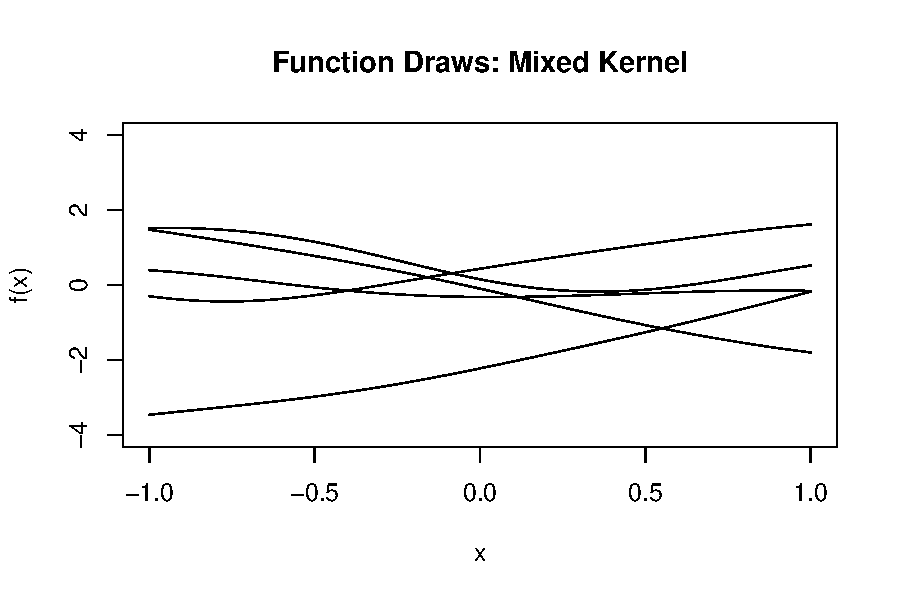
\includegraphics{fig-emulators/mixed-draws.pdf}
  \caption{Some realisations of a GP where the covariance structure is constructed by the addition of a squared exponential covariance function with a linear covariance function, as in \cref{Eq:add-covar}.}
  \label{Fig:mix-kern}
\end{figure}
\subsection{Mean functions}
The simplest mean function is $\mu(\bx) = 0$ which corresponds to the GP being ``all covariance''. GPs with a prior mean of $0$ are able to capture complex function behaviour. Generalising to $\mu(\bx) = \beta$ centres the predictions around a more useful value; the maximum likelihood estimate for $\beta$ is $\hat{\beta} = \bar{y}$ \citep{Sacks89}. But again, this is a pure covariance approach after centring the data. It can be more useful to use mean functions which depend on $\bx$ and then use a zero mean GP to model variation about this systematic mean function. That is, model the simulator output as
\begin{equation}
  f(\cdot) \sim \mathcal{GP}\{\mu(\cdot), C(\cdot, \cdot)\}.
\end{equation}
This requires a specification for $\mu(\cdot)$. An precise form may be difficult to specify (which is in part why we are using a GP), thus a popular approach is to construct the mean function hierarchically;
\begin{equation}
  \mu(\bx) = h(\bx)^T \bm{\beta}
\end{equation}
where $h(\bx)$ is a $p$-vector with each element taking a simple, deterministic form and $\bm{\beta} = (\beta_0, \beta_1, \ldots, \beta_{p-1})^T$ are unknown regression coefficients to be inferred. A common form is $h(\bx) = (1, \bx^T)$. This expresses the belief that the function is approximately linear in its inputs. Some authors are proponents of using a very simple mean functions (constant, or zero), allowing the covariance structure to do the heavy lifting \citep{Henderson09,Zhang2019}. Some prefer a complex mean function which accounts for a large amount of variability in $f(\cdot)$ and using the GP to mop up the residuals. Providing the chosen mean function is sensible, this offers robustness against an inappropriate choice for $C(\cdot, \cdot)$ and can make the emulator more interpretable \citep{Xu16,Vernon2010}. This thesis generally takes a Goldilocks approach; the mean function should aim to capture the main global trends in $f(\bx)$ whilst retaining simplicity. This can require much less effort than using a complex mean function but, despite the simplicity, can be very effective \citep{Ohagan01, Fricker2013, Fisher2021}. A different approach is to choose a complex mean form but use a prior that encourages sparsity amongst $\bm{\beta}$ to automatically choose a mean function \citep{Seshadri2020}.

\section{A general Gaussian process posterior}

\subsection{Parameter inference}
Inferring the coefficients of the mean function and the parameters of the covariance function can be done in a frequentist or Bayesian way. If useful prior information is available, \citet{Oakley2002} describes how we might elicit $\mu(\cdot)$ and $C(\cdot, \cdot)$. Suppose we have some data from the simulator. In this case, data are a set of simulator inputs and corresponding outputs. That is $\mathcal{D} = \{ (y_i, \bx_i), i = 1, 2, \ldots, n \} $ where $y_i = f(\bx_i) + \varepsilon(\bx_i)$ and $\varepsilon(\bx_i) \sim N(0, \lambda^2(\bx_i))$ models inputs dependent noise in a stochastic simulator. Commonly, the inputs $\bx_i$ are collected into a matrix $X$ where the $i$th row of $X$ is $\bx_i$. Note that setting $\lambda^2(\bx) = \lambda^2$ recovers a constant level of noise and  $\lambda^2(\bx) = 0$ recovers a deterministic function. For now we will assume that $\lambda^2(\bx) = \lambda^2 \geq 0$. Even if theoretically we should take $\lambda = 0$, because the simulator is deterministic, it often is \correction{computationally convenient to set $\lambda$ to be some small value (say $\lambda = 10^{-6}$) to avoid computational issues surrounding matrix inversion. This is just a `trick' to brush an ill-conditioned matrix under the carpet.} Some authors support estimating $\lambda$ even when the simulator is deterministic as a way to account for assumptions such as stationary or the choice of covariance being incorrect \citep{Gramacy12}. This approach is not infallible; \citet{Andrianakis2012} show this can lead to problems such as (i) bimodal likelihoods and (ii) ill-fitting emulators. Another method to avoid the problems induced by attempting to invert an ill-conditioned matrix is to use an approximate covariance matrix in place of the true covariance matrix. \correction{This might be done by using just a subset of the training data which may lead to a covariance matrix with better conditioning \citep{Wilson2015}. Yet another approximate method is a Hilbert space approximation, where a covariance function is expressed as an infinite sum, and the approximation stems from truncating the sum; this leads to approximating the GP by a linear model with basis functions (regression functions) derived from the covariance structure \citep{Solin2020, Riutort2023}.}

Regardless of whether the simulator is stochastic or deterministic, the likelihood function is then
\begin{equation}
  \by \mid \bm{\beta}, \Theta \sim \mathcal{N} \left\{ H\bm{\beta}, \Sigma\right\}
\end{equation} where the mean is constructed via multiplication of $H$, the design matrix with $j$th row $h(\bx_j)^T$ where $\bx_j$ is the $j$th vector of simulator inputs, and the coefficient vector $\bm{\beta}$. The covariance matrix is $\Sigma = C(X, X) + \lambda^2 I$, where $I$ is the identity matrix (of appropriate dimensions), $\Theta$ are the parameters of the covariance function and \correction{$C(X, X)$ is a matrix with $C(X, X)_{i,j} = C(\bx_i, \bx_j)$.} Assuming a squared exponential covariance function, and a nugget term, leads to $\Theta = (\sigma, \theta_1, \theta_2, \ldots, \theta_K, \lambda)$.  In a frequentist framework, we can maximise the likelihood function to obtain estimates $\hat{\bm{\beta}}$ and $\hat{\Theta}$ \citep{Sacks89}. \correction{In a Bayesian framework we could elicit a prior $\pi(\bm{\beta}, \Theta)$ then use numerical methods to obtain either exact or approximate samples from $\pi(\bm{\beta}, \Theta \mid \mathd)$} \citep{Svalova2021}. Alternatively,  we can maximise the posterior density to obtain \textit{maximum a posteriori} (MAP) estimates \citep{Baker2020a}. It is desirable, for computational reasons, to analytically integrate out parameters where possible. If we take $\bm{\beta} \sim \mathcal{N}(\bm{b}, B)$ this is possible. Following \citet{BDA3} (see appendix A of the reference), and noting that $\var\{H\beta\} = H B H^T$, it can be shown that we can write the distribution of $\by \mid \Theta$ as
\begin{equation}
  \by \mid \Theta \sim \mathcal{N} \left\{ H \bm{b}, \Sigma + H B^T H\right\}. \label{Eq:int-mean}
\end{equation}
   Now inference about $\Theta$ follows by treating \Cref{Eq:int-mean} as the sampling distribution for $\by$. This reduced parameter space can lead to faster inferences. From this we can obtain MLE/MAP estimates or perform a full Bayes analysis. Note that if we take $\pi(\bm{\beta}, \sigma \mid \bm{\theta}, \lambda) \propto \sigma^{-2}$ (i.e. implying infinite prior variance on $\bm{\beta}$) then both $\bm{\beta}$ and $\sigma$ can be analytically integrated out. The resulting emulator is a Student's $t$ process \citep{Oakley2002a}. \correction{The Student's $t$ process arises only from certain families of prior specification, thus a GP is often preferred.}
\subsection{Posterior predictive distribution}
A GP prior on $f(\cdot)$, $\pi(f(\cdot))$, is infinite dimensional, as is the posterior, $\pi(f(\cdot) \mid \mathcal{D})$. Both of these facts are due to there being an infinite number of choices for $\bx$. Luckily, this issue can be sidestepped. If we have a collection of $m \in \N$ new inputs, $X^{*}$, and then let
\begin{equation}
  f(X^{*}) = \begin{pmatrix}
              f(\bx^{*}_1) \\ f(\bx^{*}_2) \\ \vdots \\ f(\bx^{*}_m)
             \end{pmatrix}
\end{equation}
be the vector of (unknown) outputs at the collection of new inputs. Then we can easily find $\pi(f(X^*) \mid \mathcal{D})$. In practice, this is enough to allow us to perform any task that we would use $f(\cdot)$ for.

Now assume a mean function of the form $\mu(\bx) = h(\bx)^T \bm{\beta}$. Consider a collection of simulator outputs $\by^{(1)} = (y_1^{(1)}, y_2^{(1)}, \ldots, y_n^{(1)})^T$ at inputs
\begin{equation}
  X^{(1)} = \begin{pmatrix} \bx_1^{(1)} \\ \bx_2^{(1)} \\ \vdots \\ \bx_n^{(1)} \end{pmatrix}
\end{equation} and let the corresponding design matrix be $H_1$. Our objective will be inference about $\by^{(2)} = (y_1^{(2)}, y_2^{(2)}, \ldots, y_m^{(2)})^T$, the outputs at $X^{(2)}$ with corresponding design matrix $H_2$. After integrating out $\bm{\beta} \sim \mathcal{N}\{ \bm{b}, B\}$, we are left with the following relationship between the two sets of simulator outputs:
\begin{equation}
  \begin{pmatrix}
    \by^{(1)} \\ \by^{(2)}
  \end{pmatrix} \mid \Theta \sim \mathcal{N} \left\{
   \begin{pmatrix}
    H_1 \bm{b} \\ H_2 \bm{b}
  \end{pmatrix}, \begin{pmatrix} K(X^{(1)}, X^{(1)}) & K(X^{(1)}, X^{(2)}) \\
K(X^{(2)}, X^{(1)}) & K(X^{(2)}, X^{(2)}) \end{pmatrix} \right\}.
\end{equation}
where $K(X^{(i)}, X^{(j)}) = C(X^{(i)}, X^{(j)}) + H^{}_i B H_j^T + \diag  \{ \lambda^2 \mathbb{I}(i = j) \}$. Unless explicitly stated, $C(\cdot, \cdot)$ is used for squared exponential covariance functions and $K(\cdot, \cdot)$ represents the addition of a squared exponential, linear and white noise covariance functions (possibly with $\lambda^2 = 0$).

Then the posterior predictive distribution for $\by^{(2)}$ is also multivariate Normal \citep{Rasmussen2006Gpfm}. The mean and variance are as follows:
\begin{align}
  \E \left\{ \by^{(2)} \mid \Theta, \mathd \right\} &= H_2 \bm{b} + K(X^{(2)}, X^{(1)})K(X^{(1)}, X^{(1)})^{-1} \left( \by^{(1)} - H_1 \bm{b} \right) \label{Eq:MV1}\\
  \var \left\{\by^{(2)} \mid \Theta, \mathd \right\} &= K(X^{(2)}, X^{(2)})- K(X^{(2)}, X^{(1)})K(X^{(1)}, X^{(1)})^{-1}K(X^{(1)}, X^{(2)}).\label{Eq:MV2}
\end{align}
Observing the form of the equations we can see that the posterior mean is just the prior mean with an adjustment based on how far the prior mean, $H_1 \bm{b}$, is from the observed outputs, $\by_1$, and how correlated we expect $\by^{(1)}$ and $\by^{(2)}$ to be. The posterior variance is always \textit{less than} the prior variance and, surprisingly, is independent of the observed $\by^{(1)}$. The posterior variance depends only on the locations of simulator inputs we are interested in and their distances from the design points. However, if $\Theta$ is inferred, rather than specified, then there is a dependence on $\by^{(1)}$ via the likelihood function. Throughout this thesis, we will often refer to the ``conditional Normal equations'' which means equations with the same form as \Cref{Eq:MV1} and \Cref{Eq:MV2}. For brevity, we will denote the posterior mean at input $\bx$ by $m^{*}(\bx)$ and posterior variance at $\bx$ by $v^{*}(\bx)$.

\subsection{Specific examples}

 We will now observe how aspects of a GP prior impact the posterior. We will focus on squared exponential, linear, and white-noise covariances. We will fit an emulator to a simple, tractable example to allow us to easily compare the fit to the truth. We will work with
 \begin{equation}
   f(x) = 2 \sin (2 \pi x) + \cos(3\pi x) + 3x. \label{Eq:toy-fn}
 \end{equation}
In a more realistic scenario, the simulator is described by complex mathematical equations and implemented via many lines of computer code, thus the exact functional form is not known. We will assume a linear trend with prior mean $\E (\bm{\beta}) = \bm{0}$ and $\var(\bm{\beta}) = 2I_2$ where $I_k$ is the $k \times k$ identity matrix. Using $n = 10$ design points chosen by uniform sampling and a squared exponential covariance function with $\sigma = 3$ and $\theta = 0.5$ we can calculate the posterior distribution for any $x$ via the conditional Normal equations.
\begin{figure}[h]
  \centering
  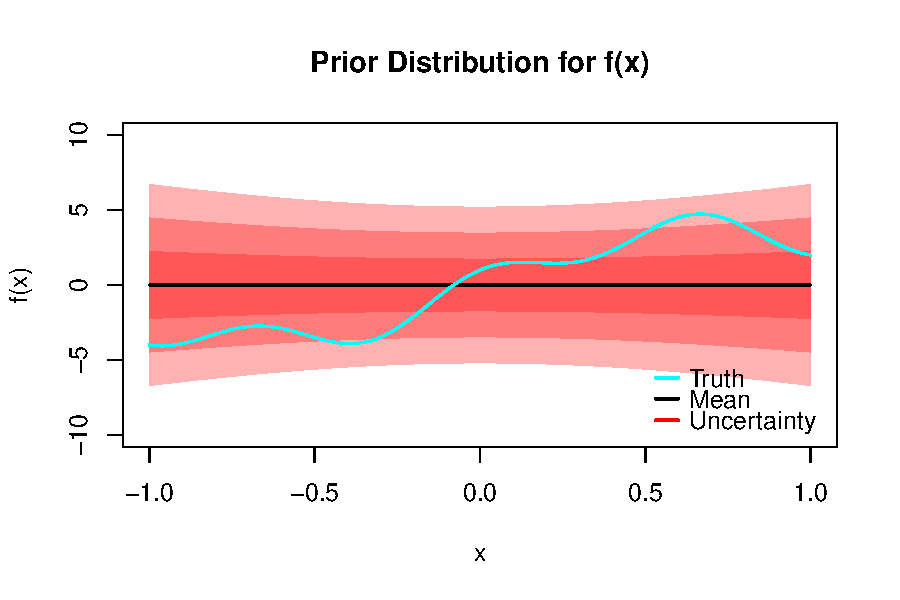
\includegraphics{fig-emulators/prior.pdf}
  \caption{Our prior specification for the simulator specified by \Cref{Eq:toy-fn}. The simulator is shown as the blue line, emulator prior mean as the black line and uncertainty is represented by the red bands; $\mu(x) \pm (1,2,3)\sqrt{K(x,x)}$.}
  \label{Fig:prior}
\end{figure}
\begin{figure}[h]
  \centering
  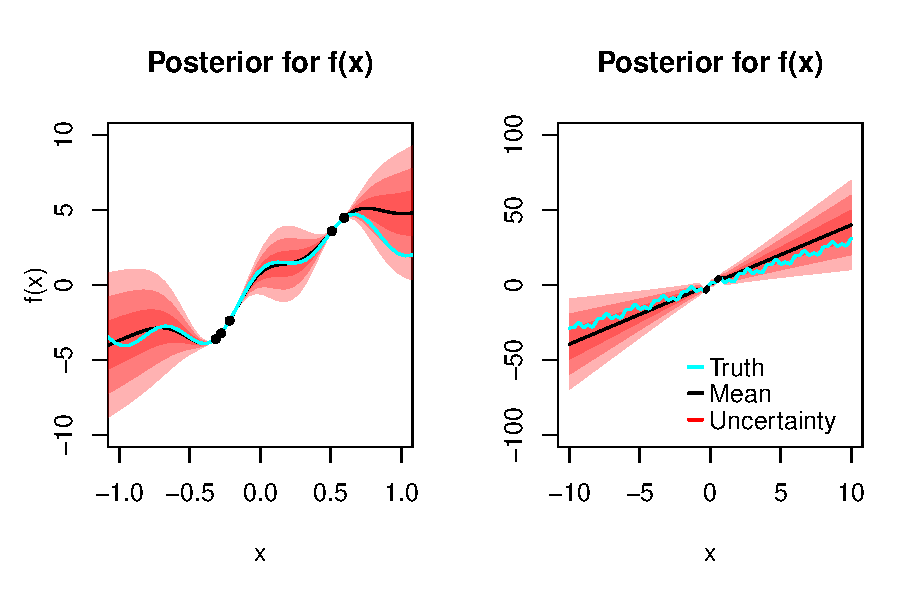
\includegraphics{fig-emulators/dual-posterior.pdf}
  \caption{The posterior distribution for the simulator specified by \Cref{Eq:toy-fn}. The simulator is shown as the blue line, the emulator posterior mean as the black line and posterior uncertainty is represented by the red bands; $m^{*} (x) \pm (1,2,3)\sqrt{ v^{*}(x) } $. The left hand plot shows how the emulator captures local variation in $f(\cdot)$ whereas the right hand plot illustrates the estimated global variation.}
  \label{Fig:posterior}
\end{figure}

An interesting feature of our prior (\Cref{Fig:prior}) is that the width of the prior predictive interval depends on $x$. Some interesting features of GP posteriors are:
\begin{itemize}
  \item[(i)] $v^* (x) = 0 \text{ and } m^*(x) = f(x) \iff x$ is a design point and $\lambda = 0$.
  \item[(ii)] $v^* (x)$ is small when $x$ is close to design points.
  \item[(iii)]  When $x$ is far from the design points, $m^*(x) \approx h(x)^T \E \{ \bm{\beta} \mid \mathd \} $.
  \item[(iv)] When $x$ is far from the design points, $v^*(x) \approx K(x,x)$.
\end{itemize}
A ``proof'' by picture of these properties is given in the the plotted posterior distribution of the synthetic example (\Cref{Fig:posterior}). The uncertainty is very small close to the training points and the mean function is close to the function values (a computational nugget $\lambda^2 = 10^{-6}$ was used here), this illustrates (i) and (ii). When we are far from the training data, the width of our posterior uncertainty bands is close to that of our prior uncertainty bands. \Cref{Fig:posterior} (left) does not clearly illustrate properties (iii) and (iv). Zooming out gives the right hand plot and shows shows that the expected response is linear, just like the prior mean function, when $x$ is far from the design points.

\subsection{Stochastic computer simulators}

It is straightforward to extend emulators to stochastic computer models. That is, those exhibiting random variation. A feature of these models is that runs of the simulator return different values even if $\bx$ remains unchanged. Our motivating example, Athena, is stochastic. This approach to simulation allows us to investigate two major sources of uncertainty:
\begin{itemize}
  \item[(i)] the stochastic nature of the world (aleatory uncertainty)
  \item[(ii)] randomising inputs to account for lack of knowledge (epistemic uncertainty).
\end{itemize}
Aleatory uncertainty is a desirable feature of models where the response is ultimately difficult to predict. For example, in the Athena simulator, aspects of the simulator are random to account for difficult to predict features such as weather and human error. Accounting for epistemic uncertainty is achieved by assigning a probability distribution to a some (or all) input parameters and propagating this uncertainty through $f(\cdot)$, usually with the help of an emulator \citep{Oakley04}.

Under stochasticity we need to be careful about what we want to infer, and hence we will be careful with our notation. Let $y(\bx)$ be the simulator output at $\bx$ and let $f(\bx)$ be the mean response at $\bx$. Under the GP framework, we perform inference on $f$ and $y$ simultaneously. We can specify their relationship hierarchically,
\begin{align}
  y(\bx) \mid f(\bx), \Theta, \bm{\beta} &\sim \mathcal{N}(f(\bx), \lambda^2) \label{Eq:homgp1} \\
  f(\cdot)  \mid \Theta, \bm{\beta} &\sim \mathcal{GP} \{ h(\cdot)^T \bm{\beta}, C(\cdot, \cdot) \}.\label{Eq:homgp2}
\end{align}
Now, since iid $\mathcal{N}(0, \lambda^2)$ noise is equivalent to the white noise covariance structure, we can integrate out $f(\cdot)$ and $\bm{\beta}$. This leads to
\begin{equation}
  y(\cdot) \mid \Theta \sim \mathcal{GP}\left\{ h(\cdot)^T\bm{b}, K(\cdot, \cdot) + \lambda^2 I \right\}
\end{equation}
where $h(\cdot)$ and $K(\cdot, \cdot)$ have their usual meanings. Note the explicit addition of the \correction{measurement error/nugget term} to $K(\cdot, \cdot)$, we have intentionally separated out the stochasticity to clarify the different between stochasticity and epistemic uncertainty. Prediction of the mean function is exactly the same as in \Cref{Eq:MV1}. Posterior variances of $y(X^*)$ and $f(X^*)$ differ only by $\lambda^2$:
\begin{align}
  \var(f(X^*) \mid \mathd, \Theta) &= K(X^*, X^*) - K(X^*, X) V^{-1} K(X, X^*)\label{Eq:varf} \\
  \var( y(X^*) \mid \mathd, \Theta) &= K(X^*, X^*)  + \lambda^2 I - K(X^*, X) V^{-1} K(X, X^*).\label{Eq:vary}
\end{align}
where $V = K(X, X) + \lambda^2 I$. \Cref{Eq:varf} allows us to make statements about $f(\bx)$ and \Cref{Eq:vary} allows us to make statements about $y(\bx)$. The difference between these two equations is analogous to the difference between a confidence interval and a prediction interval in a frequentist regression analysis.
The properties (i) and (ii) of GP posteriors do not hold here because $\lambda$ may be arbitrarily large to account for arbitrary amounts of stochasticity. Good prior information, usually specified via the mean function, can be very important in the stochastic setting since, especially if $\lambda$ is large, $y(X)$ might not be very informative for $f(X)$. We demonstrate this by adapting \Cref{Eq:toy-fn} to be stochastic. We introduce stochasticity by simulating from $y(\bx) \sim \mathcal{N} \{f(\bx), 0.5^2 \}$. This can be seen in \Cref{Fig:toy-stoch}. There is still a fairly large amount of uncertainty close to the design points. An infinite sample size is required for this uncertainty to reduce to zero. The probability bands for $y(x)$ take into account uncertainty about $f(x)$ as well as stochasticity.
\begin{figure}[h]
  \centering
  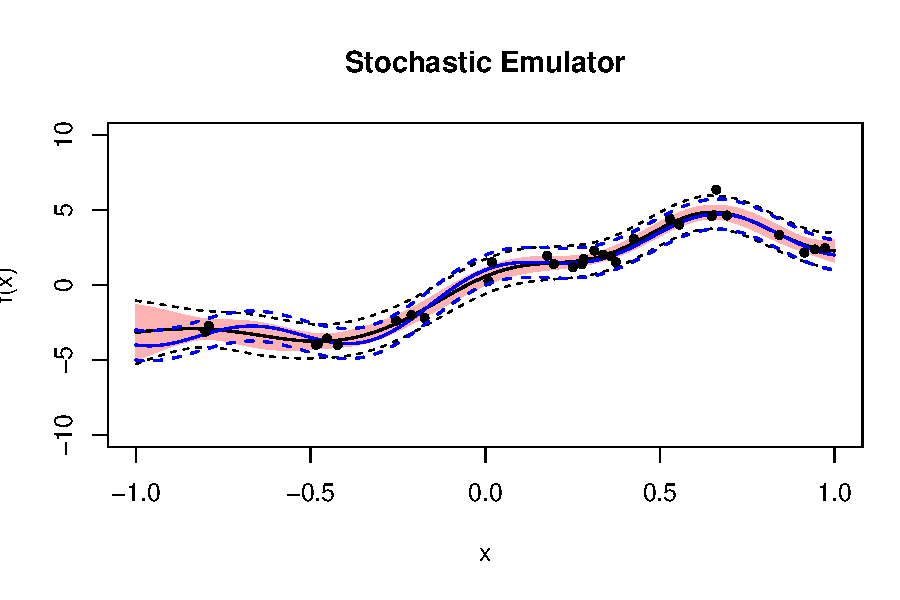
\includegraphics[width = \textwidth]{fig-emulators/toy-stoch.pdf}
  \caption{An emulator for a stochastic simulator. Solid blue line is simulator mean with blue dashed lines being $95\%$ probability bands. Solid black line is emulator mean, dashed black lines are a $95\%$ probability interval for $y(x)$ and the red band is a $95\%$ probability interval for $f(x)$.}
  \label{Fig:toy-stoch}
\end{figure}
\section{Design of computer experiments}
\correction{The previous figures in this chapter used a simple uniform sample for selecting locations at which to run the simulator.} In practice, this is usually a bad idea since \correction{randomly generated designs} can often lead to design points being very close together in space. This is wasteful since our smoothness assumptions about $f(\cdot)$ imply that \correction{$|f(\bx) - f(\bx')|$} is small whenever $||\bx - \bx'||$ is small. It therefore makes sense to spread out the design points where possible. Such designs are termed ``space filling'' designs.
Another design approach is to sequentially construct the emulator. This involves using the emulator, combined with a rule, $\alpha(\bx)$, to choose where to next run the simulator. The simulator is then run at the point satisfying $\bx^\star = \argmax_{\bx \in \mathcal{X}} \alpha(\bx)$, the emulator is updated and we repeat the process until we satisfy some stopping rule.
In general, there is no globally superior choice as to whether we go with one-shot or sequential designs, and a sequential design may be initialised by a small one-shot design \citep{Zhang2019}. One-shot designs are typically easier and cheaper to implement than sequential designs. We construct the design and run the simulator in isolation of each other. Sequential designs need the simulator and emulator to `talk' to each other, which might be difficult if the person constructing the emulator is not familiar with the language the simulator is implemented in.
\correction{Finally, one-shot designs are agnostic to choice of covariance and mean function. This can be useful in exploratory situations} where little is known about the underlying covariance function for $f(\cdot)$. For instance, \citet{Overstall2017} use a single one-shot design to construct and compare many emulators based on just one training set and one validation set. On the other hand, sequential designs can leverage our current understanding of $f(\cdot)$ (or $y(\cdot))$ to achieve specific goals more efficiently that a one-shot approach. A popular class of sequential designs, Bayesian Optimisation acquisition functions \citep{Frazier2018}, are those which aim to optimise $f(\cdot)$ whilst minimising the number of times we run the simulator. In essence, a one-shot design is a Jack of all trades, master of none, a sequential design is a master of only one.
\subsection{One-shot designs}
Perhaps the most popular one-shot designs in the computer experiments literature are Latin Hypercube (LH) designs. A LH, of size $n$ and dimension $K$, is constructed by partitioning the sample space into $n^K$ equally sized $K$-dimensional hypercubes and a single uniform sample is taken within each sub-hypercube. This leads to a `more uniform' design than truly uniform sampling. This construction allows us to guarantee that for a LH of size $n$, in each margin, there is exactly $1$ sample in each interval. This shows a clear advantage over pure uniform designs. In \Cref{Fig:rand-lh} we see a particularly unfortunate uniform design in which no samples appear above the line $x_1=x_2$ and most of the points satisfy $x_2 < 0.2$. The LH offers some protection against this, but is not watertight. For example, sampling amongst the diagonal boxes would lead to a valid LH design, but not a space filling design.
\begin{figure}[h]
  \centering
  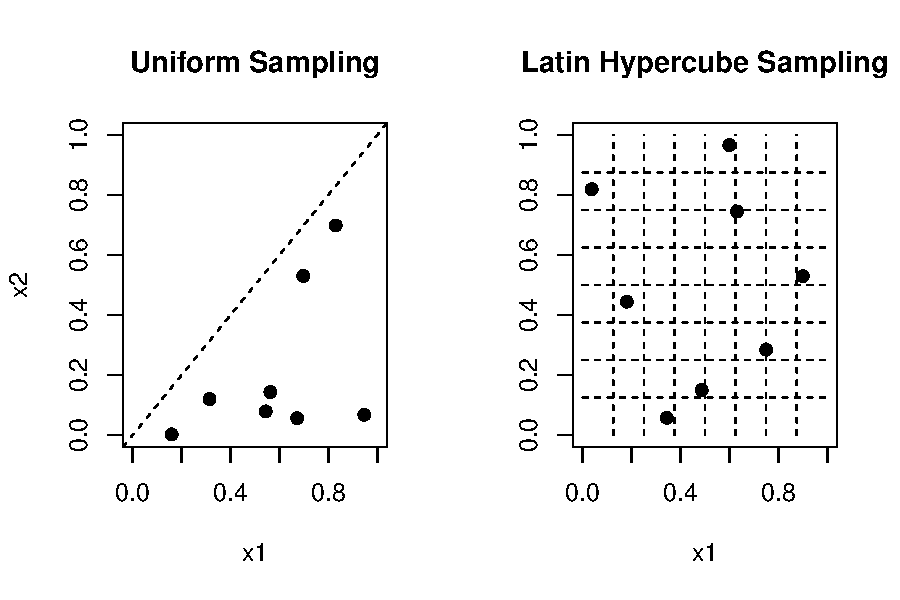
\includegraphics{fig-emulators/rand-latin.pdf}
  \caption{A $2$d random sample (left) and $2$d LH sample (right), both of size $n = 8$. In the left hand plot the dashed line corresponds to unit diagonal.  In the right hand plot, the dashed lines correspond to an $8 \times 8$ grid of equally sized sub-cubes.}
  \label{Fig:rand-lh}
\end{figure}
We can enhance LHs with additional structure to obtain a more space filling design. One such enhancement is the maximin LH. A maximin design is one which maximises the minimum distance between design points so that no pair of points are too close. This rule can be added to a LH to prevent the points sitting on the diagonal or for two points to be sitting in nearby corners of adjacent sub-cubes \citep{Mckay1979, Morris1995}.
\subsection{Sequential designs}
As discussed, sequential designs allow us to leverage our current state of knowledge to satisfy some optimality criterion. Many such designs are Bayesian since they can be expressed as expectations of random variables. For example, consider Active Learning McKay (ALM), which is based on posterior variance (and recall, the variance is the expected squared distance from the mean) \citep{Seo2000}. \correction{This method is referred to as ``uncertainty sampling'' in the machine learning literature \citep{Nguyen2022}}. If we have already run the simulator at $n$ locations, then the next point to run the simulator at, $\bx_{n+1}$, is given by
\begin{align}
  \bx_{n+1} &= \argmax_{\bx \in \mathcal{X}} \alpha_{ALM}(\bx)\\
    \alpha_{ALM}(\bx) &= v^{*}(\bx). \label{Eq:std-alm}
\end{align}
That is, we run the simulator at the location with largest uncertainty (about the underlying mean, so the variance is given by \cref{Eq:varf}) in the design space $\mathcal{X}$. The idea here is to reduce uncertainty to construct a globally accurate emulator. An approach with similar goals is to minimise the integrated mean square prediction error (IMSPE), which is given as
\begin{equation}
  \alpha_{IMSPE}(\bx) =  -  \int_{\tilde{\bx} \in \mathcal{X}} \left\{ y(\tilde{\bx}) - m^* (\tilde{\bx}) \right\} ^2 \dd \tilde{\bx}. \label{Eq:imspe}
\end{equation}
IMSPE aims to minimise the average uncertainty across $\mathcal{X}$ rather than point-wise uncertainty. This seems like a better idea than ALM, but requires integration over $\mathcal{X}$ which is difficult \citep{Gramacy2020surrogates}. \correction{A simple workaround is to approximate the integral by a sum:
\begin{equation}
    \alpha_{IMSPE}(\bx) \approx  -  \sum_{\tilde{\bx} \in X} \left\{ y(\tilde{\bx}) - m^* (\tilde{\bx}) \right\} ^2,
\end{equation}
where $X$ is a collection of design points at which the simulator has been run.} Typically, sequential designs satisfying criteria such as \cref{Eq:std-alm} and \cref{Eq:imspe} are not space filling. \correction{Sequential designs which retain similar criteria whilst also possessing space filling properties are explored by \citet{Pronzato2020}}.
\section{Model fidelity}
In many scenarios, the simulator of interest can be run at varying levels of complexity. The complexity induces a trade-off between the accuracy of simulations and the corresponding computational cost. `Cost' usually means wall clock computation time, but this could be refer to financial cost if high performance computing facilities are hired to obtain training data.
There are two main methods for constructing emulators in this scenario. One is a cumulative roughness model in which the cheapest code `level' is thought to be relatively smooth and more expensive levels are thought to have a rougher, more complex response surface \citep{Kennedy2000}. The more common type is an autoregressive model \citep{Forrester2007}, which has strong links to co-Kriging in the geostatistics literature \citep{Stein1991}. Both of these methods go by multiple names including `multilevel emulation', `multifidelity emulation' or some use co-Kriging regardless of whether the method is applied to the emulation of a simulator or a geostatistical analysis of some physical phenomena.

The core idea in both multilevel emulation and co-Kriging is that using a large, auxiliary data set, can help fill in the gaps of a sparse data set of direct interest. In geostatistics, we might have a small number of expensive, but highly accurate weather sensors placed over an area of interest. We may also have a much larger number of cheap, but inaccurate sensors placed over the same area. The cheap sensors provide a prediction of what the expensive sensors would report. We then construct a GP regression model based on the readings from cheap sensors but then perform a correction based on the expensive readings to provide an improved prediction of the weather at locations without a weather sensor. See \citet{Yates1987,Ashraf1997,Lark2007,Adhikary2017} for various examples.

This concept can be adapted to the emulation literature. In many cases, accuracy is increased by making a time step in a numerical differential equation solver smaller, or by constructing finer grids over space in spatial type models. Another scenario would be where there are two separate models; a cheap model with simple physics and an expensive model with much more complex physics.
Two methods of combining runs from these these different, but related, simulations are proposed by \citet{Kennedy2000}. Both models then become more accurate in the sense that they are better approximations of the mathematical equations being solved, they are not necessarily better approximations to reality.
\subsection{Autoregressive models}
A common approach to modelling simulators of different accuracy is via an autoregressive structure. Suppose we have a simulator $f_t(\bx)$ where $t \in \{1, 2, \ldots, T\}$ are the simulator levels. If $s>t$ then $f_s(\cdot)$ is assumed to be more accurate but also more expensive to run than $f_t(\bx)$. We assume that we have $n_{t}$ runs of each simulator; when $s > t$ we would expect that $n_s < n_t$.  This is not a mathematical constraint but rather a practical aspect of the problem. We expect to have fewer runs of the more expensive simulator, but there is no part of this framework that \textit{requires} it. \correction{We then induce the following model on the simulators:
\begin{align}
  f_1(\cdot) \mid \bm{\beta}_1, \Theta_1 &\sim \mathcal{GP}\{h(\cdot)^T \bm{\beta}_1, c_1(\cdot, \cdot)\}\\
  f_{t+1}(\cdot) &= \rho_{t}f_{t}(\cdot) + \delta_{t+1} (\cdot)\\
  \delta_t(\cdot) \mid \bm{\beta}_t, \Theta_t &\sim \mathcal{GP}\left\{h(\cdot)^T\bm{\beta}_t, c_t(\cdot, \cdot) \right\}
\end{align}}
where $\Theta_t$ are the hyperparameters of $c_t(\cdot,\cdot)$ and $\rho_t$ an autoregressive parameter. The term $\delta_{t+1}(\cdot)$ essentially represents the discrepancy between $f_t(\cdot)$ and $f_{t+1}(\cdot)$. This model relies on $f_t(\cdot)$ explaining most of the variation in $f_{t+1}(\cdot)$. It is then assumed that the $\delta_t(\cdot)$ processes are much simpler than the corresponding $f_t(\cdot)$.
If we take \begin{equation}
  c_t(\bx, \bx') = \sigma_t^2 \exp \left\{ - \sum_{i = 1}^K \frac{(x_{i} - {x_i}')^2}{\theta_{t,i}^2} \right\}.
\end{equation}
and assume that \correction{$f_t(\cdot) \indep \delta_{t+1}(\cdot)$}, then
\begin{equation}
  \cov(f_t(\bx), f_{t+1}(\bx')\mid \bm{\beta}, \Theta) = \rho_t \sigma_t^2 \exp \left\{ - \sum_{i = 1}^K \frac{(x_i - {x_i}')^2}{\theta_{t,i}^2} \right\}
\end{equation}
where $\bm{\beta} = \{\bm{\beta}_1, \bm{\beta}_2, \ldots, \bm{\beta}_T\}$ and $\Theta = \{\Theta_1, \Theta_2, \ldots, \Theta_T\}$.
The design of these multilevel experiments is interesting. \citet{Kennedy2000} shows that the likelihood is greatly simplified if $D_{t+1} \subset D_t$, that is, we run $f_{t+1}$ only at the locations which $f_t$ has been run. Rather than fitting one joint model, this allows us to fit a GP to $f_1(\cdot)$ and then to each $\delta_t(\cdot)$. In such a case, the design matrix is of the form
\begin{equation}
  H = \begin{pmatrix}
    h(X_1) & \bm{0} & \cdots & \bm{0} & \bm{0}) \\
    \rho_{(1,1)} h(X_1) & h(X_2) & \cdots & \bm{0} & \bm{0}\\
    \vdots & \vdots & \ddots & \vdots & \vdots\\
    \rho_{(1, T-1)} h(X_1) & \rho_{(2, T-1)}h(X_2) &\cdots &\rho_{(T-2, T-1)}h(X_{T-1}) & h(X_T)
\end{pmatrix}.
\end{equation}
where $\rho_{(t, s)} = \prod_{i = t}^s \rho_i$ for $s>t$. Further, conditional on all GP parameters, the covariance function for $f_t(\cdot)$ ($t \geq 2$) is
\begin{equation}
  C_t(\bx, \bx') = c_t(\bx, \bx') + \sum_{j = 1}^{t-1} \rho_{(1, j)}^2 c_j(\bx, \bx').
\end{equation}
\subsubsection{A tractable example}
Consider the computation of the following integral, viewed as a function of $x$:
\begin{equation}
  f(x) = \int_0^1 \cos(4 \pi x^2)\sin(2 \pi xt) - 4xt + 1 \diff t.
\end{equation}
This is an easy to compute integral, but if the integral was intractable, this could be replaced by a Riemann approximation:
\correction{\begin{equation}
  f_R(x; T) = \frac1T \sum_{i = 0}^{T-1} g(t_i ; x),
\end{equation}}
where $g(t ; x) = \cos(4 \pi x^2)\sin(2 \pi t x) - 4xt + 1$ is the integrand and $t_i = \tfrac{i}{T-1}$ are the equally spaced points at which $g(t;x)$ is evaluated. This integrand is cheap but in a complex computer model could be expensive to evaluate. \Cref{Fig:fidelity} shows how increasing $T$ improves the approximation. We see when $x>0.4$ and $T=2$ the cheap approximation is a poor approximation to the analytical solution; the local maxima and local minima swap places. For $T \geq 4$ the approximation improves, but with diminishing returns.
\begin{figure}[h]
  \centering
  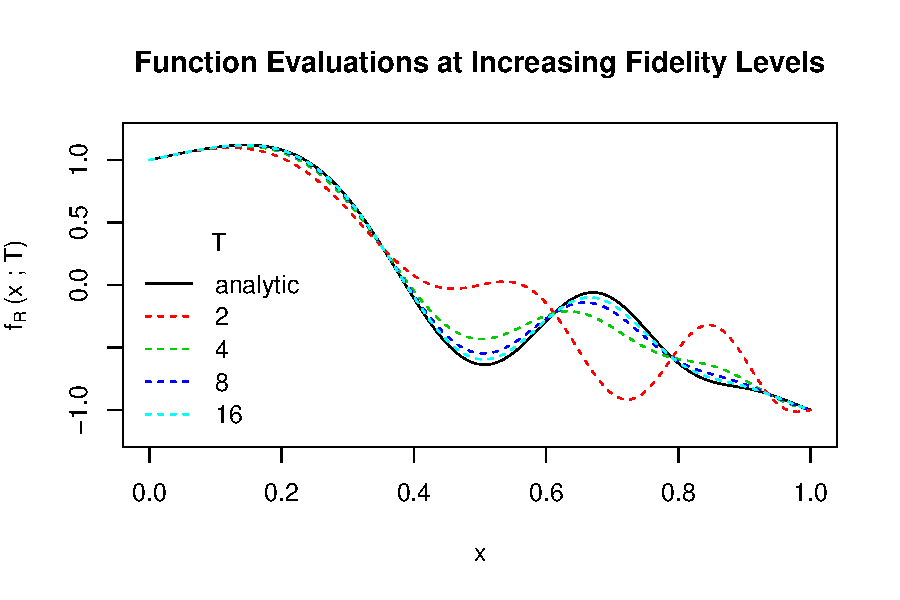
\includegraphics{fig-emulators/fidelity.pdf}
  \caption{Solutions to $f_R(x;T)$ at different fidelity levels. Approximate solutions are given by dashed lines, the analytic solution is given by the solid line. $T$ corresponds to the number of evaluations of $g(t;x)$ in the Riemann integration.}
  \label{Fig:fidelity}
\end{figure}
Suppose we have $n_e = 3$ evaluations of $f_R(x; 40)$ but also have $n_c = 20$ evaluations of $f_R(x;4)$. The evaluations of $f_R(x;4)$ may have been from a trial, exploratory run of the simulator or chosen to help us emulate $f_R(x; 40)$.
\begin{figure}[h]
  \centering
  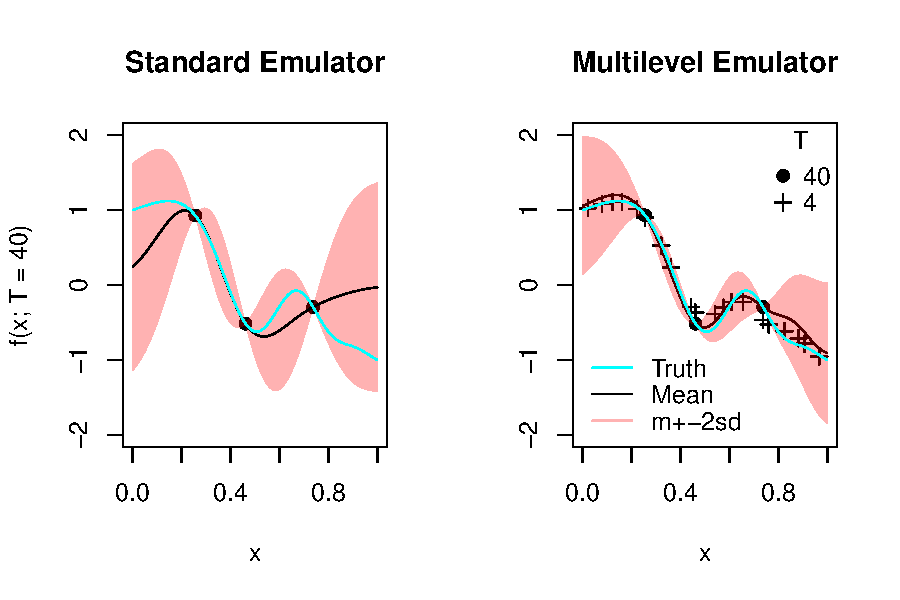
\includegraphics{fig-emulators/compare-ml.pdf}
  \caption{A standard GP emulator (left) and corresponding multilevel emulator (right). Here, the `truth' refers to $f_R(x;40)$, the object of inference, rather than the analytic solution.}
  \label{Fig:compare-ml}
\end{figure}
We see, qualitatively, that the multilevel emulator offers an improved fit over the standard emulator (\Cref{Fig:compare-ml}). Firstly, the mean function more closely reflects the truth, this is especially noticeable once we start extrapolating beyond the range of the observed expensive data. There is also a moderate reduction in uncertainty about the expected function value, reflecting that the auxiliary information from a different level of code \textit{is} informative for a more expensive version. In this toy, $1$-dimensional example, it is easy to see that the multilevel emulator is better.

\correction{If our most accurate simulator level is still too coarse, one may be interested in producing a multilevel emulator that mimics the effect $T \to \infty$. That is, emulates the exact mathematical model rather than the code. Recent ideas from probabalistic numerics --- a field of statistics and machine learning which phrases numerical solutions as inference problems --- have been shown to be effective at emulating the case $T \to \infty$; we do not discuss this any further but direct the reader to \citet{Teymur2021} for further reading.}

\section{Emulator comparison}
When fitting an emulator in a higher dimensional space, it is much trickier to assess fit. We will now demonstrate some emulator performance metrics on the standard GP and the multilevel emulator from \cref{Fig:compare-ml}. Here we consider the use of two performance metrics to assess the emulator. The first is root mean squared error (RMSE). Given a set of set of `unseen' data $\mathcal{D}_{\text{test}} = \{ (\bx_{\text{test},i}, y_{\text{test},i}), i = 1, 2, \ldots, n_{\text{test}} \} $, this can be found via
\begin{equation}
  RMSE = \sqrt{ \frac{1}{n_\text{test}}  \sum_{i = 1}^{n_\text{test}} \left\{ y_{\text{test},i} - m^*( \bx_{\text{test},i} )  \right\}^2 }. \label{Eq:rmse}
\end{equation}
RMSE only considers how close $m^{*}(\cdot)$ is to $f(\cdot)$. This does not take into account the uncertainty about $f(\cdot)$ or $y(\cdot)$, which motivates the use of a proper scoring rule. Proper scoring rules reward forecasts with high certainty when they are accurate but do not heavily penalise inaccurate forecasts when they have a large uncertainty attached to them \citep{Gneiting2007}. For GP emulators, the following scoring rule (bigger is better) is commonly used \citep{Binois2018,Jackson2019}
\begin{equation}
  S(\mathcal{D}_\text{test}) = -\frac{1}{n_{\text{test}}}\sum_{i = 1}^{n_\text{test}}\left\{ \frac{[y_{\text{test},i} - m^*(\bx_{\text{test},i} ) ]^2}{v^*(\bx_{\text{test},i})} + \log v^*(\bx_{\text{test},i})\right\}.\label{Eq:scoring-rule}
\end{equation}
\Cref{Eq:scoring-rule} is essentially the point-wise log-likelihood based on a Normal distribution. \correction{Although the predictions are thought to be correlated, for a small and well spaced test set, the predictions should be approximately independent.}

Returning to the multilevel emulators, we compute the RMSE and score for each emulator based on the two proposed metrics based on $100$ equally spaced test points. This is a very large number of test points relative to the design. In practice, the size of the test set would likely be no larger than the training design. There does not appear to be any literature on appropriate sizes for test designs, but types of design have been explored \citep{Challenor2013}.

\Cref{Tab:toy-ml-metric} gives the two pairs of performance metrics for the competing emulators. The RMSE for the multilevel emulator is much smaller than the standard emulator, this is expected since \cref{Fig:compare-ml} showed that the emulators mean for the multilevel emulator was almost the same as the target function. The score also shows a healthy improvement under the multilevel approach, this tells us that, in a combined sense, the posterior distribution provided by the multilevel emulator is a better probabilistic prediction than the posterior distribution provided by the standard emulator.
\begin{table}[h]
\centering
  \begin{tabular}{rll}
    \toprule
    Emulator & RMSE & Score \\ \cmidrule{1-3}
    Standard&$0.4292$&$1.917$\\
    Multilevel&$0.1139$&$3.588$\\
    \bottomrule
  \end{tabular}
  \caption{Performance metrics for two the standard and multilevel emulators in \Cref{Fig:compare-ml}.}
  \label{Tab:toy-ml-metric}
\end{table}
\section{Emulator diagnostics}
As with any statistical model, we must investigate whether the emulator is an appropriate approximation to the simulator. The main emulator diagnostics, for deterministic simulators, were proposed by \citet{Bastos09} (from hereon in, BO'H). A similar set of diagnostics have been proposed by \citet{Baker2019a} for stochastic simulators.
Here we review the diagnostics proposed by BO'H that are used later in this thesis. However, BO'H integrate out $\sigma$ in their emulators, resulting in the posterior being a Student's $t$ process. We will always conditions on $\sigma$, thus the posterior is Gaussian. Therefore, the diagnostics we present have been adapted to assume a GP posterior.
\subsection{The diagnostics}
The diagnostics all rely on Cholesky Errors (C.E.s). These are analogous to standardised residuals in a standard regression analysis but take into account the covariance structure of the emulator. This is important since, we expect \correction{$|f(\bx) - f(\bx')|$} to be small whenever $||\bx - \bx'||$ is small. In other words, we expect the residuals to have structure even when the emulator is an appropriate representation of the simulator. The C.E.s are defined to be
\begin{equation}
  \bm{e}_{\text{chol}} = \Sigma_\text{test}^{-1/2}(\by_{\text{test}} - m^{*}(X_{\text{test}}))
\end{equation}
where $m^*(X_{\text{test}})$ is the emulator's posterior mean vector and $\Sigma_\text{test}$ is the posterior variance matrix for the test points. $\Sigma^{-1/2}_\text{test}$ is the inverse of the lower Cholesky decomposition of $\Sigma_\text{test}$. If the emulator is an adequate approximation to the simulator then $\bm{e}_\text{chol}$ should appear as a random sample from $\mathcal{N}_{n_\text{test}}(0, I)$ when plotted against $x_{\text{test},i}$. We can perform further diagnostics based on these residuals. Since they are (supposedly) a random sample from $\mathcal{N}(0,1)$, a QQ-plot can be constructed to assess Normality, as can a coverage plot which compares
\begin{equation}
  C_\alpha (\bm{e}) = \frac{1}{n}\sum_{i=1}^n \mathbb{I} ( e_i \in I_{\alpha})
\end{equation}
to various values of $\alpha$. Here, $I_\alpha$ is a (symmetric) interval in which $100(1-\alpha)\%$ of the C.E.s are expected to lie. In the Normal case, $I_\alpha = \left( \Phi(\frac{\alpha}{2}), \Phi (1 - \frac{\alpha}{2}) \right)$.
\subsection{Example}
We will work with the $2$-dimensional toy function that BO'H use:
\begin{equation}
  f(\bx) = (1-e^{-0.5x_2^{-1}})\left( \frac{2300x_1^3 + 1900 x_1^2 + 2092 x_1 + 60}{100 x_1^3 + 500x_1^2 + 4x_1 + 20} \right), \bx \in (0,1)^2.
\end{equation}
We then constructed a $20$ point LH on $(0,1)^2$, fit the emulator using the same parameters as BO'H; $\sigma^2 = 3.3316$, $\bm{\theta} = (0.2421, 0.4240)$ and we used a nugget effect of $\lambda^2 = 10^{-16}$ (BO'H did not explicitly use a nugget term, but we have included one for computational reasons). A second, independent LH of size $20$ was constructed to generate a test set of data. We also assumed a linear mean function but with with $\bm{\beta} \sim N(\bm{0}, 100I_3)$ rather than the improper prior $\pi(\bm{\beta}) \propto 1$. The C.E.s then lead to a suite of diagnostic plots (\Cref{Fig:diags}). It is clear from the plots that there is serious emulator-simulator discrepancy. When $x_1$ and $x_2$ are both less than about $0.3$ there are some very large C.E.s (around $6$ in magnitude). This is reinforced by the the QQ-plot; the points do not lie close to the line. For a small sample size the coverage plots can be highly non-smooth, but we can see there is a `flat line' of observed coverages around $0.8$ indicating a gap in the coverages. This also suggests serious emulator-simulator discrepancy.
 \begin{figure}[h]
   \centering
   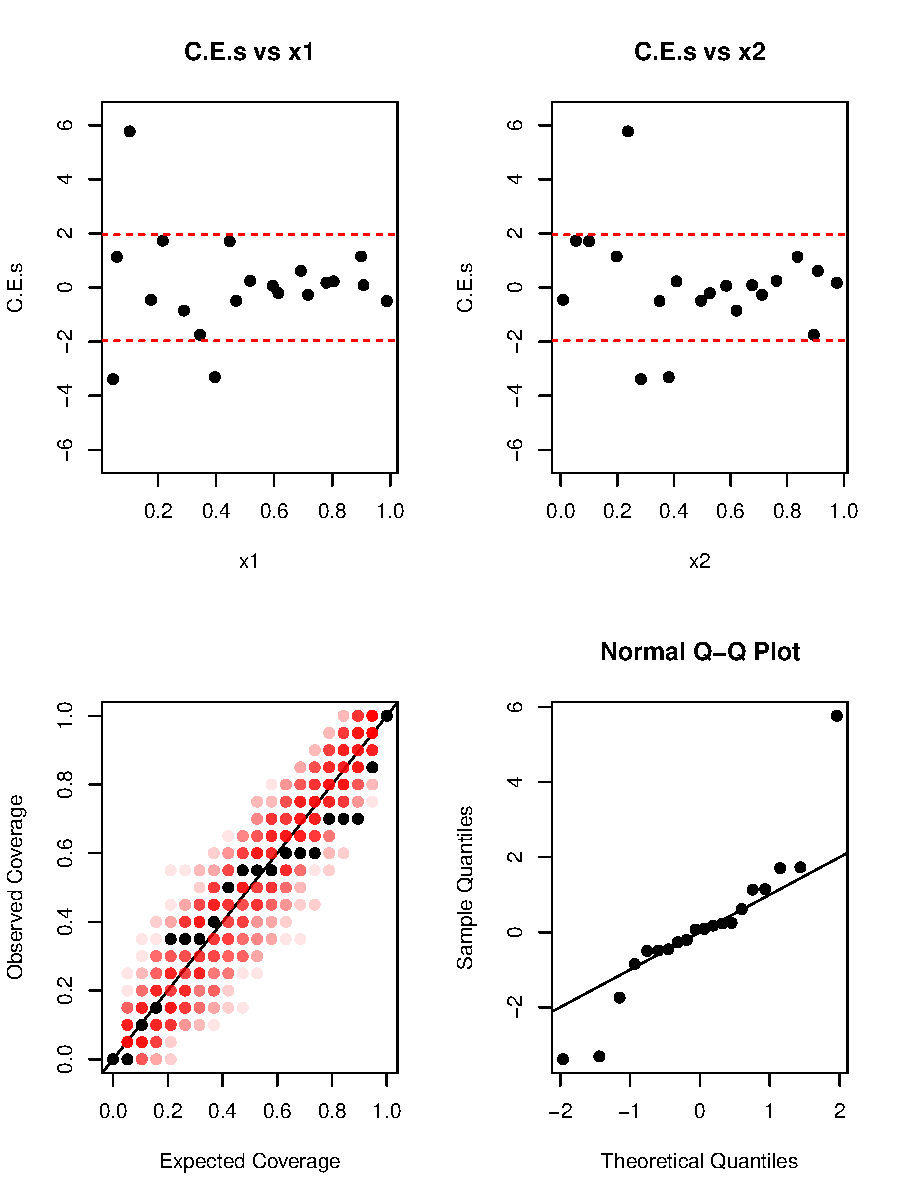
\includegraphics{fig-emulators/diags.pdf}
   \caption{Diagnostic Plots for the toy emulator. Top two plots are C.E.s against the inputs (left is input $1$, right is input $2$). Bottom right shows a QQ plot with the unit diagonal superimposed. Bottom left is the coverage plot, black points correspond to observed C.E.s, translucent red dots correspond to the coverage observed from $100$ iid $\mathcal{N}(0,1)$ samples of size $20$.}
   \label{Fig:diags}
 \end{figure}
To improve the emulator we will follow BO'H and generate some additional data points and update the GP hyperparameters. If the simulator were very expensive this might not be possible. If further simulator runs are not possible, we can try other methods to improve the emulator. Common approaches include changing the mean function \citep{Overstall2016} and/or covariance function to to better reflect the simulator behaviour \citep{Volodina2020,Vernon2022tense}.
We generate an additional $10$ points from an independent LH design on $(0, 0.5)^2$ in an attempt to build a satisfactory emulator. We update the hyperparameters to the values BO'H used; $\sigma^2 = 4.9389$, $\bm{\theta} =  (0.1764, 0.4116)$. The emulator is then refit leading to the diagnostics in \Cref{Fig:diag2}. The diagnostics are much improved; there are no very large C.E.s (we have one $|e_i|>1.96$, but this is expected in a sample of size $20$). There is no striking systematic pattern in the residuals, perhaps there is some indication of decreasing variance as the $x_i$ increase but this is hard to judge with a small sample size. The QQ-plot shows good fit to the line and the coverage plot is within the realms of what we would expect from a sample of size $20$.
\begin{figure}[h]
  \centering
  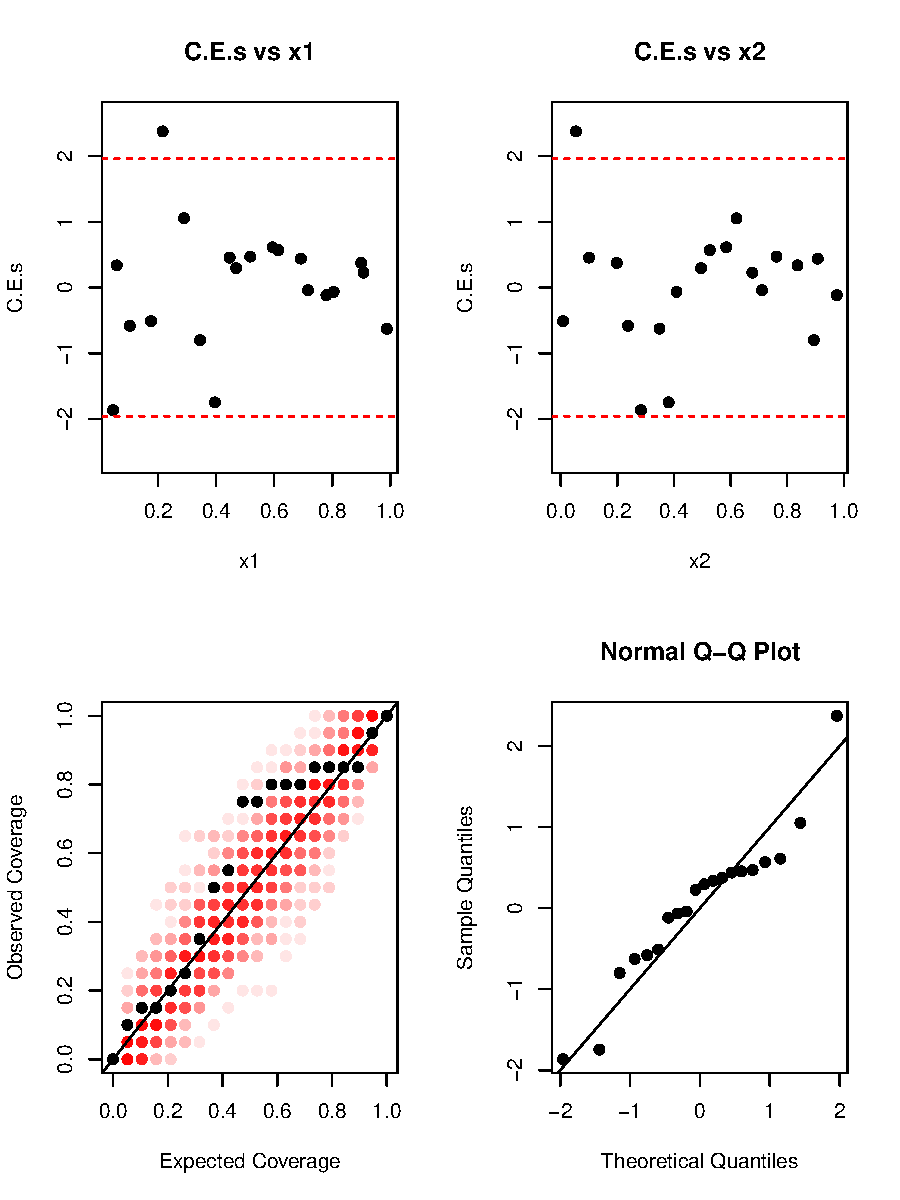
\includegraphics{fig-emulators/diag2.pdf}
  \caption{Diagnostic Plots for the toy emulator. Top two plots are C.E.s against the inputs (left is input $1$, right is input $2$). Bottom right shows a QQ plot with the unit diagonal superimposed. Bottom left is the coverage plot, black points correspond to observed C.E.s, translucent red dots correspond to the coverage observed from $100$ iid $\mathcal{N}(0,1)$ samples of size $20$.}
  \label{Fig:diag2}
\end{figure}
\section{Other surrogate models}
Emulators do not have to be GPs. Other approaches have different advantages to GPs. For example, if the simulator inputs are permutations, the size of $||\bx - \bx'||$ implies little about \correction{$|f(\bx) - f(\bx')|$.} In permutation space, a Benter model inspired emulator offers a promising solution \citep{Wilson2018}. Most non-GP surrogates do leverage some kind of smoothness about $f(\cdot)$ and thus re-purpose conventional regression techniques. Examples include generalised additive models, neural networks and splines \citep{Marrel2012, Tripathy2018, Barton2006}. We now discuss two non-GP emulators in turn.
\subsection{Linear models}
\correction{Linear regression (Bayesian or frequentist) offers a much faster inference and prediction framework than GPs with, for example, squared exponential or Mat\'ern covariance structures, \citep{Rougier2009}.} This is because GP inference usually relies on inverting a matrix, an $\mathcal{O}(n^3)$ operation. Prediction, given a GP precision matrix is then $\mathcal{O}(n^2)$. For fully Bayesian treatments with $S$ Markov chain Monte Carlo (MCMC) samples, predictions are typically $\mathcal{O}(S n^3)$, where S is fairly large ($S \geq 10^4$). Inference is more costly still, in part to due mixing and thinning of MCMC schemes. For example, \citet{Baggaley2012} needed $550K$ MCMC iterations \textit{after} a series of trial MCMC schemes used to tune their sampling scheme. \correction{Under certain prior assumptions, the posterior distribution of a linear regression is fully tractable, thus complex computations such as matrix inversion need to be performed only once.} One interpretation of the linear regression emulator is a type of emulator with a covariance that is ``all nugget''. The advantage of GPs over linear regression is that GPs automatically detect otherwise difficult to model features in the data, so the human cost of linear modelling --- fitting many different functional forms, including interaction and polynomial terms --- may be greater than the cost of inverting a matrix. The choice between linear regression and GP is context dependent; \citet{Salter2016} explore this in detail and find merits in both approaches.
Although a simple approach, this can work quite well in both the stochastic and deterministic settings. For example, even when the simulator is deterministic, a nugget term is often incorporated. This might be a very small nugget for computational reasons or a larger nugget as a way to account for deviations from assumptions \citep{Gramacy12}. Another reason is that the fitted emulator might only depend on a subset of the variables fed into the simulator. This means that the emulator has a random component to account for the information `lost' by omitting unimportant variables from the emulator, thus a nugget is required almost always regardless of whether we have a stochastic or deterministic emulator.
\subsection{Bayes linear emulators}
Bayes linear emulators \citep{Jones2016, Wilson18, Bower2010, Vernon2019, Jackson2023} come from a framework which is, in principle, Bayesian. The prior specification is greatly simplified as the prior specification is only of means and (co)variances. In the Bayes linear framework we want to update our beliefs about a vector of beliefs $B$ having observed a data vector $D$. Following \citet{BLS07} the ``posterior'' (known as \textit{adjusted}) mean and (co)variances are given by
\begin{align}
  \E_{D}(B) &= \E(B) + \cov(B, D) \var(D)^{-1}(D - \E(D)) \label{Eq:bl-mean}\\
  \var_{D}(B) & = \var(B) - \cov(B, D) \var(D)^{-1} \cov(D, B) \label{Eq:bl-var}.
\end{align}
These formulae bear a striking resemblance to the conditional Normal equations. Despite the resemblance, they have an important but subtle distinction from the conditional Normal equations. The conditional Normal equations are the posterior moments \textit{of a Normal distribution} and thus imply precise probability statements about $f(\bx)$. The Bayes linear equations are distribution free statements (in terms of both the likelihood and prior) thus are not making precise probability statements. Proponents of a Bayes linear analysis claim this simplified specification allows for a more robust analysis because we are not tied to probability statements. The downside is that it might be harder to interpret a Bayes linear emulator. With a GP emulator, if $f(\bx) \sim \mathcal{N}(0, 1)$ then we can make statements such as $\p (f(\bx)>0) = 0.5$, whereas a Bayes linear emulator will not offer this level of detail. It is possible to make imprecise probability statements by feeding the adjusted moments into certain results from probability theory such as Pukelsheim's $3\sigma$ rule \citep{Pukelsheim1994} or Markov's inequality. Neither approach is necessarily better, the advantages and disadvantages of each paradigm should be weighed up and it is indeed valid to mix the two approaches to leverage the benefits of each. One example of a mixed approach is \citet{Owen2020}; a (truncated) GP emulator and a Bayes linear emulator are used together to emulate a simulator exhibiting different behaviour patterns.

Ultimately, a Bayes linear analysis produces a central estimate and quantification of uncertainty in an efficient way, which is all that is often needed from an emulator. A Bayes linear analysis can be thought of as either an approximate Bayesian analysis or the appropriate analysis when we are only willing to specify means and (co)variances. Since \Cref{Eq:bl-mean} corresponds to \cref{Eq:MV1} and \cref{Eq:bl-var} corresponds to \Cref{Eq:MV2}, \correction{the Bayes linear approach works exceptionally well when $B$ is approximately Normal, but offers a valid analysis when $B$ is non-Normal.} In the Bayes linear framework, we would usually take $D = y(X)$ and $B = y(X^*)$ (or $f(X^*)$) and $\cov(B, D)$ and $\var(D)$ can be found via assuming an appropriate covariance function, such as a squared exponential. This allows for a Bayesian emulator whilst avoiding MCMC schemes or other approximations. Although not strictly confined to the Bayes linear framework, proponents of the Bayes linear framework typically use emulators of the form
\begin{equation}
  f(\bx) = \sum_{j = 1}^q \beta_j h_j(\bx_{[A]}) + w(\bx_{[A]}) + \varepsilon(\bx)
\end{equation}
where $\bx_{[A]}$ are the ``active'' inputs (the subset of inputs thought to be most influential on simulator output), $\sum_{j = 1}^q \beta_j h_j(\bx_{[A]})$ is a mean function, $w(\cdot)$ is a mean-zero weakly stationary stochastic process and $\varepsilon(\cdot)$ is a white noise process. In this formulation, $w(\cdot)$ is analogous to a (mean zero) GP in the fully Bayesian setting, thus we write $\cov\{w(\bx^{}_{[A]}), w(\bx'_{[A]})\}  = C(\bx^{}_{[A]}, \bx'_{[A]})$. The mean function is often very detailed which means that --- if $f(\bx)$ is well approximated by $h(\bx)^T \bm{\beta}$ --- there is a reduced reliance on choosing the correct form for $C(\cdot, \cdot)$. A more detailed mean function may allow the emulator to be more interpretable, as the regression function is more understandable than the non-parametric component of the emulator \citep{Bower2010, Vernon2019}.
\section{Summary}
The purpose of this chapter was to motivate and establish the core concepts used later in the thesis. We began with the central concept of this thesis; an emulator. That is, a GP approximation to a simulator. We introduced the notion of a GP as a prior distribution over functions. We described how to encode certain prior beliefs about $f(\cdot)$ through this prior; we considered some common covariance structures for emulators and how these each imply different prior specifications for an unknown function. We also examined the effects of combining covariance structures. Multiplication of covariance structures typically leads to multiple input emulators; addition of covariance structures allows us to build emulators with different components.  We also discussed mean functions and evaluated the pros and cons of mean functions of different complexities.

We then moved to posterior inferences and design strategies for $f(\cdot)$. The multivariate Normal equations were presented as our path to an analytic posterior, conditional on GP hyperparameters; we discussed some approaches to estimation of both the hyperparameters and regression coefficients. We had a fleeting discussion of stochasticity; this will be greatly expanded upon in the next chapter. We contrasted one-shot and sequential designs and with a bias towards constructing space filling designs. \cref{Chap:optimisation} will discuss some sequential design approaches in greater detail with a particular emphasis on optimisation as a sequential problem.

The final GP emulator we considered in this chapter was an autoregressive emulator which used one cheap code level to improve both the emulation of a more expensive level of code, with a comparison to co-Kriging in geostatistics. We presented a concrete example of a two-level emulator but presented mathematical details of how to extend to an arbitrary number of levels. We then showed, via appropriate metrics, that the multilevel emulator out performed a standard emulator. We closed the consideration of GP emulators by presenting a suite of appropriate diagnostics for GP emulators.

We concluded this chapter on emulators by considering some approaches to emulation \textit{not} based on GPs. The first was linear regression based emulation, and the other was Bayes linear emulation. Although both are different to GP emulation, they can both have strong links. Linear regression can be thought of as a GP emulator based on linear and white noise covariance functions. We saw that the multivariate Normal equations are mathematically identical to the Bayes linear update equations.
\end{chapter}

  \begin{chapter}{Heteroscedastic \& Multilevel GP Emulators For Stochastic Simulators\label{Ch:Hetsml}}

The work in this chapter has been written up as a paper and recently accepted for publication in \emph{Journal of the Royal Statistical Society: Series C (Applied Statistics)} \citep{Kennedy2023}. \correction{The main contribution of this paper is the introduction of the stochastic multilevel (SML) emulator. A secondary contribution of this paper is comparing algorithms to fit SML emulators, as well as comparing algorithms to fit HetGP emulators, which SML emulators are a natural extension of.}
\section{Introduction}
The previous chapter focused on using GP priors to model complex computer simulators. We reviewed many of the classical emulation strategies which were developed between the $1980$'s and early $2000$'s. This literature focused on \textit{deterministic} simulators, since, at the time, they were the most common type of simulation model \citep{Sacks89,Craig1997, Ohagan01, Santner2003}. These deterministic models were implemented even if the corresponding real world process exhibited stochasticity \citep{Ohagan01}. Of course, this absent stochasticity is `wrong', as are all models. Nonetheless, these deterministic models still have practical value.

To incorporate uncertainty into predictions, modellers have produced increasing numbers of stochastic simulators. As stochastic simulation has become more prominent across all sciences, so has the interest in the emulation of stochastic computer simulators \citep{Henderson09, Astfalck19, Rocchetta2018, Boys2018}. There are a variety of approaches to (GP based) emulation of stochastic computer models; see \citet{Baker2022} for a recent overview.

The simplest approach to modelling stochastic simulators, which was outlined in the previous chapter, is to add $\lambda^2 I$ to the covariance structure. This homoscedastic approach is rather limiting when $\var\{ y(\bx) \}$ is thought to depend on $\bx$. A canonical example of heteroscedasticity is the `motorcycle data', which comes directly from a stochastic computer experiment \citep{Schmidt1981}. This computer experiment outputs accelerometer readings over time following a crash. Although \citet{Silverman1985} fits splines to this data, we will use GPs and start with a homoscedastic GP (HomGP).
\begin{figure}[ht]
	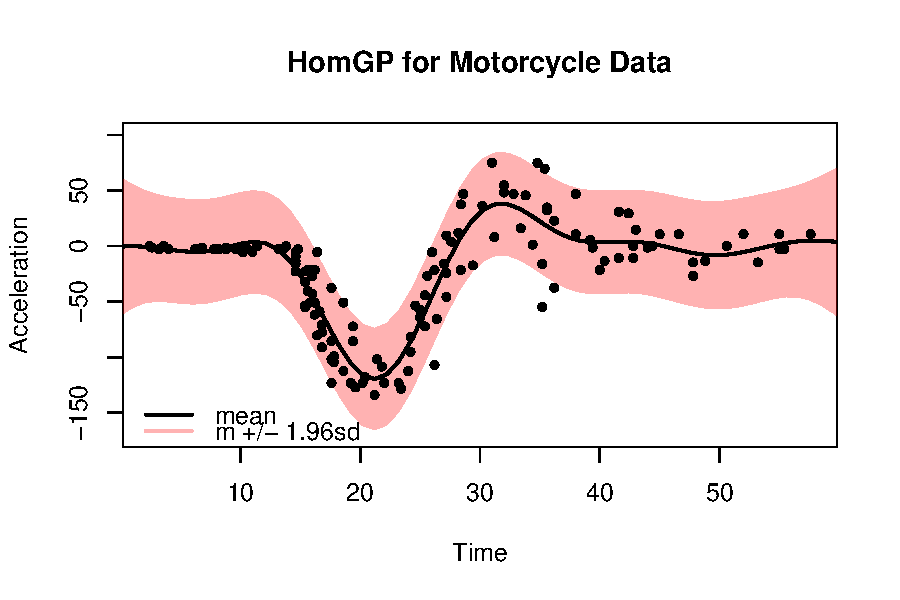
\includegraphics{fig-het-sml/mcycle-homgp.pdf}
	\caption{The motorcycle data set with HomGP superimposed. The black line is the emulator mean and the red band corresponds to a $95\%$ posterior predictive interval for $y(x)$.}
	\label{Fig:mcycle-hom}
\end{figure}

The fitted mean function in \Cref{Fig:mcycle-hom} for the motorcycle data is reasonable. The pitfall is that the emulator's predictive variance is a poor match for the variability in the data, thus interval estimates for $y(\bx)$ are poorly calibrated. There will also be a knock-on effect on uncertainty quantification for $\E \{ y(\bx) \}$. The misspecified variance is most prominent for $\text{Time}<15$, where it is clear that $\var \{y(\bx) \}$ is very small but the emulator estimates $\var\{ y(\bx) \mid \mathcal{D}) \approx 28$. The predictive variance also looks too large for $\text{Time}>40$. The predictive variance is reasonably accurate for $\text{Time} \in [15, 40]$. Ultimately, to produce surrogates for heteroscedastic simulators, we need to produce emulators with a heteroscedastic element baked into them. Our goal here is to find an approach which can:
\begin{itemize}
	\item[(i)] produce a mean estimate of $y(\bx)$;
	\item[(ii)] quantify uncertainty about $\E \{ y(\bx) \} $;
	\item[(iii)] provide flexible estimates of $\lambda^2(\bx) = \var\{ y(\bx) \}$.
\end{itemize}
\section{Separate mean and variance emulation}
To estimate the mean response of a heteroscedastic stochastic simulator, we might apply Stochastic Kriging (SK) to runs of the simulator \citep{Akenman2010}. SK is similar to the constant noise set up. The difference being that instead of having a (prior) covariance matrix of the form $\var\{y (X)\} = C(X, X) + \lambda^2 I$, we have
\begin{equation}
	\var\{y (X)\} = C(X, X) + \diag\left( \frac{s^2(\bx_1)}{r_1},\frac{s^2(\bx_2)}{r_2}, \ldots, \frac{s^2(\bx_k)}{r_k} \right)
\end{equation}
as the covariance matrix, where $s^2(\bx_i)$ is the (sample) variance based on $r_i$ replicated runs of $y(\bx_i)$. For SK it is recommend that $r_i \geq 10$. This deals with the heteroscedasticity at the design points since the nugget term depends on $\bx$. However, the noise is treated as a nuisance rather than as an object of inference; SK only emulates $\E \{ y(\bx) \}$. Emulating stochastic computer models can be viewed as modelling a multiple output simulator. If both outputs (mean and variance) are important, then we need to explicitly model $\lambda^2(\bx)$.

\citet{Henderson09} construct two independent GP emulators: one for $\E \{y(\bx) \}$ and another for $ \log \lambda(\bx)$. Note that \citet{Henderson09} emulate the log standard deviation, rather than log variance, but these are identical up to a multiplicative factor of $2$. Their case study employs around $1000$ replicates per design point; this does not take too long for their example (they generate their training data in about a day using parallel computing) but for more expensive simulators this may be an unachievable sample size. Simple sample mean and standard deviation estimates are used as the training data to construct their emulators. This independence assumption is pragmatic; the simulator mean and standard deviations are both functions of $\bx$, but it is a practical and useful modelling choice. A very similar approach is adopted by \citet{Andrianakis2017} and is shown to be more powerful, in terms of increasing the efficiency of an calibration procedure, than taking $\lambda^2(\bx) = \lambda^2$.

\citet{Marrel2012} take a similar approach to \citet{Henderson09} but couple together their mean and variance GPs. They first estimate the mean response using a HomGP. Let the posterior mean be $m_0(\bx)$. Next they estimate $\var\{ y(\bx) \} \approx \frac{1}{r} \sum_{i=1}^r (y_i(\bx) - m_0(\bx))^2$ and fit a GP to the estimated variances. Let the posterior mean of this GP be $m_V(\cdot)$. They then fit a new GP to $y(\bx)$ using $m_V(\cdot)$ in place of $\lambda^2$: $y(\cdot) \sim \mathcal{GP} \{ m(\cdot), C(\cdot, \cdot) + m_V(\cdot)I \}$. The authors suggests that this approach may be improved by alternating between the fitted variance GP and the mean GP until some convergence criterion is met.

\subsection{Non-Gaussian noise}
If the stochasticity exhibited by $y(\bx)$ is not well approximated by a Normal distribution (e.g. asymmetric), then more work may have to be done. Transformation is a simple but effective method for addressing non-Normality. For example, if it is known that $y(\bx) > 0$ a log transform may be enough to rectify non-Normality. The availability, $A(\bx)$, in Athena is constrained to the unit interval thus, constructing an emulator for $\logit A(\bx)$ or $\probit A(\bx)$ would be a sensible strategy.

If the simulator behaviour is too complex to be made (approximately) Gaussian by transformation, Quantile Kriging may be an appropriate tool \citep{Plumlee2014}. Since quantiles are directly estimated, rather than moments, Quantile Kriging is very flexible and can reproduce complex simulator behaviour such as multimodal outputs and discrete outputs without additional modelling. This is perhaps the most flexible approach to modelling stochastic simulators. This flexibility comes at a large cost; hundreds of replicates are required to model non-Gaussian, input dependent noise in computer simulators. Many stochastic simulators, such as Athena, can be computationally expensive. Thus such levels of replication could make emulation of the Athena, and other simulators, infeasible unless huge training budgets are available.

Another approach to using GPs to model simulators which are asymmetric or otherwise non-Normal is to embed a GP into another statistical model. This is an attractive approach since it may help leverage problem structure. For example, if a model outputs an integer (perhaps, the number of cells that have mutated in a biological system), we may wish to model the response as $y(\bx) \sim \text{Poisson}\,(\gamma(\bx))$ with $\log \gamma (\cdot) \sim \mathcal{GP} \{m(\cdot), C(\cdot, \cdot) \}$. Note the lack of nugget term in the GP because the stochasticity is absorbed into the Poisson error structure (this is also true for many non-Gaussian models which utilise a GP). A Bayesian treatment would require intensive numerical methods to integrate out the latent GP to form the posterior density for $y(\bx)$ in this Poisson model. For this reason, the person constructing the emulator may prefer to employ the tractable and computationally efficient GP over a more accurate, but unwieldy, non-Gaussian emulator. For example, the capture-recapture example illustrated in \citet{Baker2022} is non-Gaussian, but the (computational) advantages of employing a GP surrogate outweigh this misrepresentation of the simulator.

If the response is non-Gaussian, but all that is required is a central estimate and quantification of uncertainty, then a Bayes linear approach may be useful. If probabilistic predictions are required, the adjusted moments can be plugged into a parametric form. For example, \citet{Jackson2019} use a Bayes linear emulator to find the adjusted mean and variance of a simulator, then plug these moments into (i) a Normal distribution and (ii) a uniform distribution to construct probabilistic predictions for a deterministic simulator. This approach of plugging moments into a parametric form can easily be adapted to stochastic simulations. However, those utilising a Bayes linear approach typically prefer not to assume any probabilistic form and report only the adjusted moments.

\section{Heteroscedastic Gaussian processes}

The approaches considered so far in this chapter typically rely on using multiple emulators to generate predictions for a single quantity of interest; $y(\bx)$. There is something inherently dissatisfying about requiring two \correction{independent statistical} models to make predictive statements about a single quantity of interest. A unified approach is appealing.

Unification of mean and variance emulators motivates the Heteroscedastic Gaussian Process (HetGP), which originated in the machine learning literature as a regression procedure \citep{Goldberg1998} but has recently gained traction in the emulation literature for modelling simulators exhibiting input dependent noise \citep{Binois2018, Baker2020c}.

\subsection{The HetGP emulator}

If $y(\cdot)$ is a stochastic computer model, then the HetGP emulator is as follows:
\begin{align}
y(\cdot) | \lambda^2(\cdot) &\sim \mathcal{GP} \{ \mu(\cdot), C(\cdot, \cdot) + \lambda^2(\cdot) \} \label{Eq:} \\
\log \lambda^2 (\cdot) &\sim \mathcal{GP} \{ \mu_V (\cdot), C_V (\cdot, \cdot) + \lambda_{V}^2 I \}.
\end{align}
An alternative representation is $y(\cdot) = f(\cdot) + \sqrt{\lambda^2(\cdot)} \varepsilon$ where $f(\cdot) \sim \mathcal{GP}\{ \mu(\cdot), C(\cdot, \cdot) \}$, $\log \lambda^2(\cdot) \sim \mathcal{GP}\{\mu_V(\cdot), C_V(\cdot, \cdot) + \lambda_V^2I \}$ and $\varepsilon \sim \mathcal{N}(0, 1)$.

Here, $\mu(\cdot)$ and $C(\cdot, \cdot)$ are mean and covariance functions (respectively) for $f(\cdot) = \E \{y(\cdot)\}$. $\mu_V(\cdot)$ and $C_V(\cdot, \cdot)$ are the mean and covariance functions for $\E\{ \log \lambda^2(\cdot) \} $ and $\lambda_V^2 I$ denotes a constant nugget effect for the log variance. Now $\var(y(\bx)) = C(\bx, \bx) + \lambda^2(\bx)I$ depends explicitly on $\bx$ even if $C(\cdot, \cdot)$ is a stationary covariance function, thus HetGP is a type of non-stationary GP. \citet{Boukouvalas2010} proposed simplifying HetGP by replacing the GP prior on $\log \lambda^2 (\cdot)$ by a known parametric form with parameters to be inferred.

A unique property of HetGP is that it need not require replication, but still allows for it. The allure of HetGP is the promise of a full surrogate; joint prediction of the mean response and the level of noise at any input combination. This is possible via a latent variable formulation which jointly models the simulator mean as a GP and the log noise (to ensure positivity) as a GP. As \citet{Gramacy2020surrogates} notes, this coupled GP approach provides smooth estimates of the noise at both within sample and out of sample simulator inputs.

As with the previous chapter, we will assume squared exponential covariance functions for $C(\cdot, \cdot)$ and $C_V(\cdot, \cdot)$, but this is not a requirement. The \texttt{hetGP} package allows for other covariance functions such as Mat\'ern \citep{hetGP}. Notation for the simulator mean, $f(\cdot)$, will be the same as in the previous chapter. The equivalent notation for $\log \lambda^2 (\cdot)$ will have a $V$ subscript. To our knowledge, no previous work on using HetGPs considers parameter uncertainty in a tractable format; \citet{Goldberg1998} propose a suitable MCMC scheme for full Bayesian computation. In the next section we outline our partially Bayesian HetGP, which does not require intensive computation for inference or prediction.
\subsection{A Bayesian HetGP}
Our approach to a tractable, but Bayesian, HetGP is to integrate out the $\bbeta$ parameters of all regression components in the two GPs. First consider the latent log-variance GP:
\begin{equation}
	\log \lambda^2(\cdot) \mid \bbeta_V, \Theta_V \sim \mathcal{GP} \{ h_V(\cdot)^T \bbeta_V , C_V(\cdot, \cdot) + \lambda^2_V I\}
\end{equation}
where $\Theta_V$ are the hyperparameters of $C_V(\cdot, \cdot)$ and the nugget variance; that is $\Theta_V = \{\sigma_V, \bm{\theta}_V, \lambda_V\} $. Since this is a homoscedastic GP, if we take the prior $\bbeta_V \sim \mathcal{N}\{\bm{b}_V, B_V \}$ then by standard properties of multivariate Normal random variables we arrive at
\begin{equation}
	\log \lambda^2(X) \mid \Theta_V \sim \mathcal{GP} \{ H_V \bm{b}_V , C_V(X, X) + H_V B_V H_V^T + \lambda^2_V I\}
\end{equation}
where the $i$-th row of $H_V$ corresponds to $h_V(\bx_i)$. As with the GPs presented in \cref{Ch:Emulators} we will use the notation $K(\cdot, \cdot)$ to represent a covariance function after integrating out regression coefficients. A $V$ subscript is used when referring to aspects of $\log \lambda^2 (\cdot)$. The posterior moments of $\log \lambda^2(\cdot) \mid \Theta_V$ are a direct consequence of the multivariate Normal equations. Prediction of $\log \lambda^2(X^{*})$ at new points $X^*$ with design matrix $H^{*}_V$ is given by:
\begin{align}
	\log \lambda^2(X^*) \mid \Theta_V, \log \lambda^2(X) &\sim \mathcal{N} \{ m^*_V(X^*), v_V^*(X) \} \label{Eq:bayes-post-lambda} \\
	m_V^*(X^*) &= H^*_V \bm{b}_V - K_V(X^*, X) K_V(X, X)^{-1} (\log \lambda^2(X) - H_V \bm{b}_V)\\
	v_V^*(X^*) &= K(X^*, X^*) - K_V(X^*, X) K_V(X, X)^{-1} K_V(X, X^*) + \lambda^2_V I
\end{align}
\correction{which relies on estimates of $\log \lambda^2 (X)$, the values of the (log) latent variance process. In practice, these cannot be observed unless replication is present. Within a Bayesian framework, estimating $\log \lambda^2 (X)$ is automatic since it is simply an unknown. As with any other unknown, we can express prior beliefs about $\log \lambda^2(X)$ and then estimate $\log \lambda^2(X)$ using standard estimation techniques. A MAP estimate can be found if a point estimate is sufficient. More intensive methods, such as MCMC, will allow us to obtain a distribution for $\log \lambda^2 (X)$ if necessary. In \cref{sec:ppd} and \cref{sec:fitting}, we provide some practical information about estimating $\log \lambda^2 (X)$.}

Then our model for the observable $y(\bx)$ is
\begin{equation}
	y(\cdot) \mid \bbeta, \Theta, \lambda^2(\cdot) \sim \mathcal{GP} \{ h(\cdot)^T \bbeta, C(\cdot, \cdot) + \lambda^2(\cdot)I \}, \label{Eq:gp-for-y}
\end{equation}
where $\Theta$ denotes $\Theta_V$ and all the hyperparameters of the GP in \cref{Eq:gp-for-y}, namely, $\Theta = \{\Theta_V, \sigma, \bm{\theta} \}$. Now we can integrate out $\bbeta \sim \mathcal{N}(\bm{b}, B)$ in the usual way leading to
\begin{equation}
	y(X) \mid \Theta, \lambda^2(\cdot) \sim \mathcal{N} \{ H\bm{b}, K(X, X) + \lambda^2(X)I \}
\end{equation}
where $K(X, X) = HBH^T + C(X, X)$ is the covariance function of $\E \{y(X)\}$ after integrating out $\bbeta$. Under this approach, we need to obtain a point estimate of $\lambda^2(\bx)$ from \cref{Eq:bayes-post-lambda}. Obvious candidates are the posterior mean, median and mode of $\lambda^2(X^*)$. Since $\log \lambda^2(X)$ is Normal, $\lambda^2(X)$ is log Normal and thus:
\begin{align}
	\E \{\lambda^2(X^*) \mid \mathcal{D}, \Theta \} &= \exp \{ m_V^*(X^*) + \frac{1}{2}v_V^*(X^*) \}\\
	\text{mode}\, \{\lambda^2(X^*) \mid \mathcal{D}, \Theta \} &= \exp \{ m_V^*(X^*) - v_V^*(X^*) \}\\
	\text{median}\, \{\lambda^2(X^*) \mid \mathcal{D}, \Theta \} &= \exp \{ m_V^*(X^*)\}.
\end{align}
 The most conservative estimate is the mean, whereas the mode will be the most optimistic. All three will be approximately equal when $|v_V^*(X^*)|<<|m^*_V(\bx)|$. Thus, if the variance is much less than the magnitude of the mean, we would recommend using the median point estimate as this does not rely on $v_V^*(X^*)$ thus is fastest to compute. The speed difference will be greatest for larger sample sizes, and typically $v_V^*(X^*)$ will be small for large sample sizes. Also small values for $\sigma_V$ and $\lambda_V$ lead to small $v_V^*(X^*)$.
\subsection{Returning to the motorcycle example}
Returning to the motorcycle example, \Cref{Fig:mcycle-het} presents a HetGP fitted to the motorcycle data. The predictive intervals provided by the HetGP emulator are more appropriate than those from the HomGP emulators. The interval width is small for $\text{Time} < 15$, is wider when $15 < \text{Time} < 30$ and then shrinks again when $\text{Time} > 30$, mimicking the input-dependent variability in the data.
\begin{figure}[ht]
	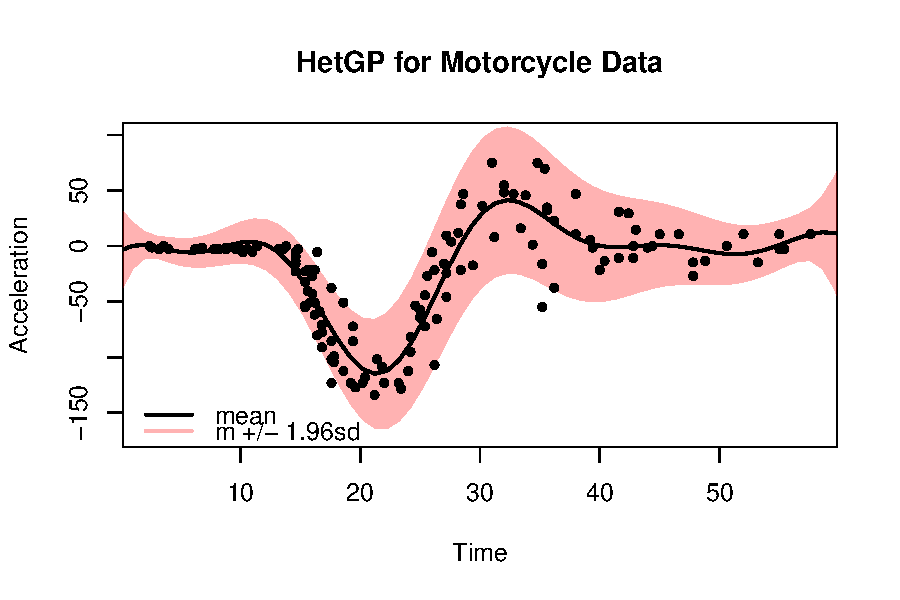
\includegraphics{fig-het-sml/mcycle-hetgp.pdf}
	\caption{The motorcycle data set with a HetGP superimposed. The black line is the emulator mean and the red band corresponds to a $95\%$ posterior predictive interval for $y(x)$.}
	\label{Fig:mcycle-het}
\end{figure}
HetGPs are great at detecting non-linear variability in both the mean response surface of a simulator and the variance surface. However, it is incredibly data-hungry; \citet{Binois2018, Zhang2022} both used hundreds of runs per input dimension; the single input motorcycle example has a sample size of $133$.

\subsection{Shortcomings of HetGP \label{hetgp-shortcomings}}
We often construct emulators because the data (simulator runs) are scarce. Let us consider a simple, tractable and heteroscedastic stochastic simulator, defined for $x \in [0,1]$:
\begin{align}
	y(x) &= 4\sin(7 \pi x) + 5(2x + 1) + 3 \log (x + 0.01) + (5x + 2)\varepsilon\label{Eq:toy-stoch}\\
	\varepsilon &\iid \mathcal{N}(0,1).
\end{align}
This simulator is simple and virtually instantaneous to run, thus is used only for illustrative purposes.
\begin{figure}[ht]
	\centering
	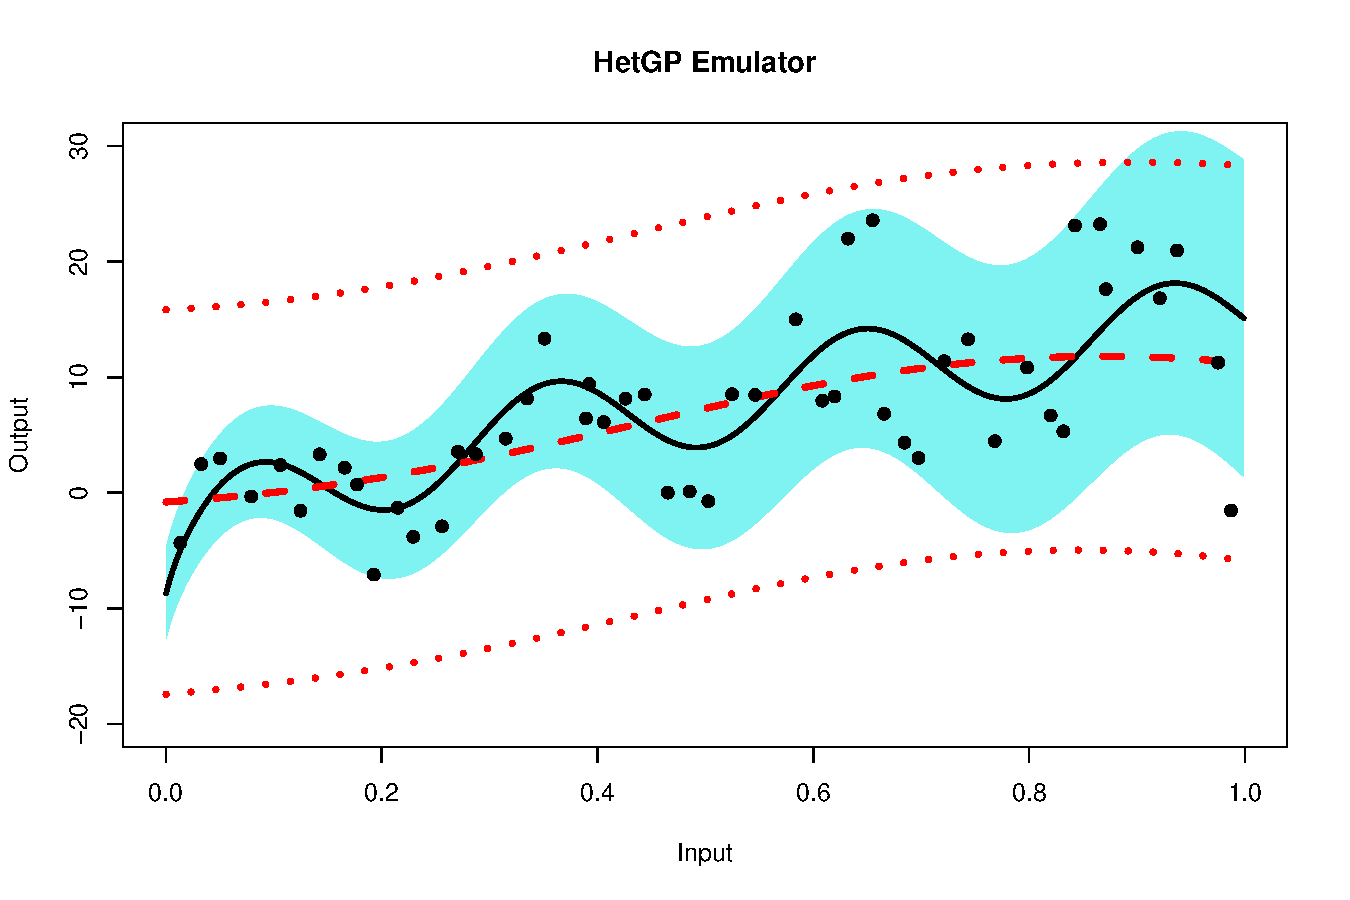
\includegraphics[width=\textwidth]{sml-het-fig2/toy-hgp.pdf}
	\caption{A HetGP emulator for \Cref{Eq:toy-stoch}. Black points are the outputs from $50$ runs of the simulator. Black line represents the true simulator mean and the blue band represents the mean $\pm 1.96$ `true' standard deviations. Red dashed line represents emulator mean with red dotted lines being the emulator mean $\pm 1.96$ emulator standard deviations. 	\label{Fig:toy-HetGP}}
\end{figure}
We constructed a HetGP emulator for \cref{Eq:toy-stoch} using $50$ design points. Observing the fit in \Cref{Fig:toy-HetGP}, the fitted emulator mean (dashed red line) does not match up well with the simulator. The emulator predicts an approximately linear response, whereas the simulator is clearly sinusoidal in nature. The emulator is interpreting the systematic sinusoidal variation as noise, rather than signal. Ultimately, this is because emulating a stochastic computer model requires much more information than the standard deterministic problem. However, when provided with adequate amounts of data, HetGP can produce excellent surrogates for complex stochastic computer models \citep{Binois2018}. The confusing of signal and noise is a similar phenomenon to that observed by \citet{Andrianakis2012}, they observed that $(\lambda, \theta)$ often have a bimodal likelihood when emulating deterministic simulators, with one mode corresponding to large $\lambda$. In other words, it is not uncommon for the emulator to favour an overly smooth fit. There are essentially three ways in which a HetGP can interpret variability in a stochastic simulation:
\begin{itemize}
	\item[(1)] Low signal; high noise. In this case $\lambda^2(\cdot)$ is over-estimated, resulting in an overly-smooth mean response. This is what has happened in \Cref{Fig:toy-HetGP}.
	\item[(2)] Low noise; high signal. This is where $\lambda^2(\cdot) \to 0$ and the mean function interpolates the data as if the simulator were deterministic.
	\item[(3)] A Goldilocks fit, i.e somewhere in between the other two. In this case, the HetGP will manage to separate the noise from the signal and produce an appropriate fit akin to \Cref{Fig:mcycle-het}.
\end{itemize}
When simulator runs are sparse, it is quite easy to end up in scenario (1). In our experience, (2) is very rare, but is still possible. To end up in (3), the ideal scenario, we need to either have a relatively large number of simulator runs to allow HetGP to tease the signal from the noise or elicit strong and accurate beliefs about $y(\cdot)$ expressed via $\mu(\cdot)$ and $C(\cdot, \cdot)$. However, if $y(\cdot)$ is a complicated simulator which implements cutting-edge science, there may be limited knowledge of appropriate choices for $\mu(\cdot)$ and $C(\cdot, \cdot)$. It is commonly the case that we are emulating $y(\cdot)$ to perform inference about $\mu(\cdot)$.
\section{Stochastic multilevel emulation\label{sec:SML}}
On many occasions, HetGPs require a lot of information, either expressed through a prior specification which accurately reflects simulator behaviour, or in the form of large amounts of training data, to produce an adequate approximation to the simulator under study. To satisfy the appetite of HetGP we can provide HetGP with runs from a related, but cheaper, version of the simulator under study. This motivates the stochastic multilevel (SML) emulator proposed in \citet{Kennedy2023}, which we will discuss, implement and compare to HetGP. We also compare two estimation routines for the HetGP and SML emulators.
\subsection{Motivation and intuition}
In the Athena simulator it is simple to change model features to give us cheap approximations to large offshore wind farm simulations. Since these approximations are relatively computationally cheap, we can use these approximations to get enough training data to construct good emulators. If we can build a good emulator for the cheap simulator, and accurately describe its mean, perhaps we can utilise this information to build better emulators for more expensive versions of the stochastic computer models.

Exploiting cheap approximations to an expensive simulator has been tackled in the deterministic framework by \citet{Kennedy2000}. The most popular format is their autoregressive structure for functions \citep{Forrester2007, Singh2017, Harvey2018}. The autoregressive structure builds a well informed emulator for the cheap simulator and uses this as a ``starting point'' for the expensive simulator. The main aim of multilevel emulation is an improved emulation of the simulator at a fixed training budget. We extend this approach to the more complex case of stochastic computer experiments and use it to enhance the emulation of the Athena simulator.

In this section, we outline our proposed approach to stochastic multilevel (SML) emulation of stochastic simulators. This naturally extends deterministic emulation techniques and exploits the cheap approximations that are readily available from the Athena simulator. Although our application is within engineering, multilevel emulation for agent based models, which are often heteroscedastic, has been identified as a useful technology \citep{Swallow2022}. We therefore propose a general approach that will apply to many stochastic simulators when cheap approximations are available. Many stochastic computer simulators have a complexity parameter, such as the length of a time step, or granularity of a grid over space, which exchanges simulation accuracy for computational cost; examples include \cite{Kennedy2000} and \citet{Le2014}. In our wind farm setting this will be the time step, $\Delta t$, in the numerical integration used to solve \cref{Eq:intensity} many times within each simulation run.

 The number of event times is affected by $\Delta t$, which generates the random time between events. Accurate runs ($\Delta t = 0.001$) of the Athena simulator take just over $3$ minutes for a wind farm with $200$ turbines on a desktop PC with $8 \times 3.20 \,\text{GHz}$ processors and $16\,\text{GB}$ RAM. On the same machine, cheap runs ($\Delta t = 0.1$) take just under $3$ seconds. A single expensive run is computationally equivalent to $60$ cheap runs. The accuracy required comes at a computational cost which severely limits the size of our computer experiment, reducing the quality of the fitted emulator. We aim to exploit these computational properties in jointly modelling the ``cheap'' simulator and ``expensive'' simulator. The outputs from cheap and expensive versions of stochastic simulators will be related. Runs from both versions are combined to build an overall better emulator.

 The two levels of the Athena simulator are approximately linearly related; see \Cref{Fig:cheapandexp}. The relationship is not exact, partially due to the stochasticity of the two levels. The relationship flattens off when the probit cheap code exhibits values above about $1.6$.
\begin{figure}[ht]
 \centering
 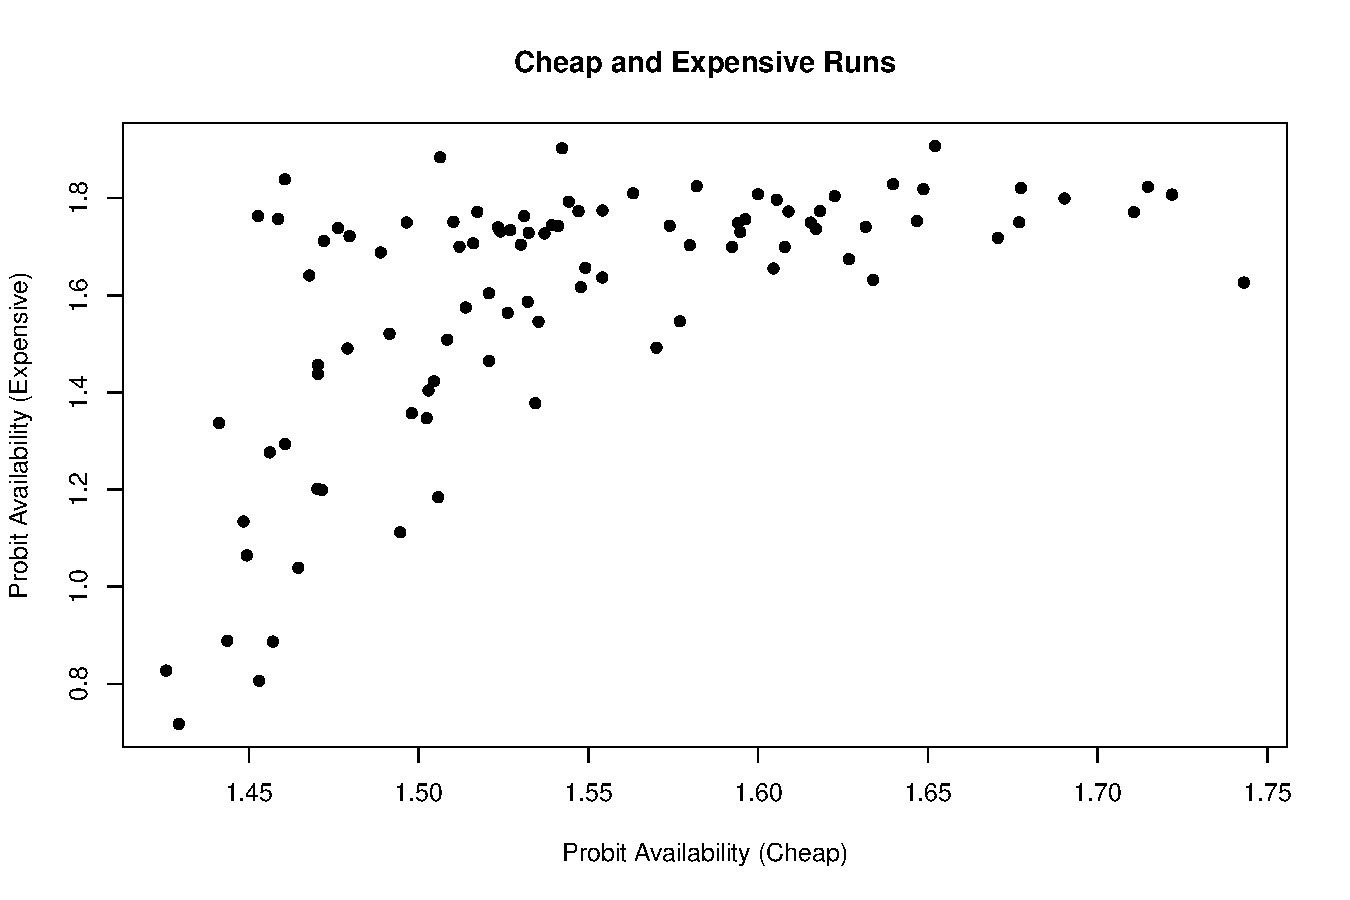
\includegraphics[width=0.75\textwidth]{sml-het-fig2/cheapVexp.pdf}
\caption{Mean probit availability under the expensive version plotted against the cheap version. Each point is computed via $10$ replications. We see an approximately linear relationship between the two levels of code but note that the range of the axes is quite different: $0.7<\text{Expensive}<2$ but $1.4<\text{Cheap}<1.8$. }
 \label{Fig:cheapandexp}
\end{figure}
We will focus on a two level set up; $y^C(\cdot)$ is the cheap simulator and $y^E(\cdot)$ is its expensive counterpart. In the motivating example of the Athena simulator $y^C(\cdot)$ is a version of the model with a time step of $\Delta t = 0.1$ years ($\approx 1$ month). We want to infer $y^E (\cdot)$, which is a version with time step $\Delta t = 0.001$ years ($\approx 9$ hours).
\subsection{Proposed emulation strategy}
We allow for $y^E(\cdot)$ to be heteroscedastic, but if we believe it is homoscedastic we can replace the non-constant variance with a constant term \citep{Roth2022}. Our object of inference is (the distribution of) $y^E(\bx)$, for any $\bx$.

Suppose that the cheap simulator, $y^C(\cdot)$ can be modelled by a homoscedastic (constant noise) GP with mean function $m_C(\cdot)$, covariance function $C_C(\cdot, \cdot)$ and constant variance $\lambda^2_C$, that is,
\begin{equation}
	y^C(\cdot) \sim \mathcal{GP} \left\{ m_C(\cdot), C_C(\cdot, \cdot) + \lambda^2_C I\right\},
\end{equation}
or equivalently, $y^C(\cdot) = Z^C(\cdot) + \varepsilon^C(\cdot)$ where $Z^C(\cdot) \sim \mathcal{GP}\{m_C(\cdot), C_C(\cdot, \cdot)\}$ and $\varepsilon^C(\cdot) \sim \mathcal{GP}\{ 0, \lambda^2_C\mathbb{I}(\cdot, \cdot)\}$.

We expect that the cheaper simulator's mean is informative for the expensive counterpart and thus, as in \cite{Kennedy2000}, we assume that
\begin{equation}
	y^E(\cdot)|\rho, Z^C(\cdot), \delta(\cdot) = \rho Z^C(\cdot) + \delta(\cdot)
\end{equation}
where $y^E (\cdot)$ is the expensive stochastic simulator and $\delta(\cdot)$ is a HetGP such that
\begin{align}
	\delta(\cdot)|\lambda_E^2 (\cdot) \sim \mathcal{GP}\left\{ m_E(\cdot), C_E(\cdot, \cdot) + \lambda^2_E(\cdot)I \right\} \\
\log \lambda^2_E(\cdot) \sim \mathcal{GP} \left\{ m_V(\cdot), C_V (\cdot, \cdot) + \lambda_{V}^2 I \right\},
\end{align}
where the $I$ are identity matrices of appropriate dimensions. It is also convenient to decompose $\delta(\cdot)$ into a deterministic component and a stochastic component; $\delta(\cdot) = Z^E(\cdot) + \varepsilon^E(\cdot)$ where $Z^E(\cdot) \sim \mathcal{GP}\{m_E(\cdot), C_E(\cdot, \cdot)\}$ is the deterministic component and $\varepsilon^E(\cdot) \sim \mathcal{GP}\{0, \lambda^2(\cdot)\}$ is the stochastic component.
In this formulation, $\rho \in \R$ is a regression parameter and $m_E(\cdot)$, $C_E(\cdot, \cdot)$ are mean and covariance functions for $\delta(\cdot)$. The term $\delta(\cdot)$ serves a dual purpose. Firstly, $\delta(\cdot)$ can be viewed as a discrepancy function; the mean of $\delta(\cdot)$ represents the difference in the mean response of the two simulators, or the loss of accuracy from running cheap simulations (with a large time step/coarse grid). Secondly, $\delta(\cdot)$ describes the stochasticity in the expensive simulator. This is a similar structure to that of Bayesian calibration of deterministic computer models \citep{Ohagan01}, however we do not observe data from a physical system --- but a computer simulator --- and we have noise in both sets of observations.

This joint model for the two simulators allows us to borrow information from the cheaper simulator, but is sufficiently flexible to reject a relationship between the two levels if no such relationship exists. If $\rho = 0$ we recover HetGP.

We express the mean functions in a hierarchical form so that	$m_C(\bx) = h(\bx)^T \bm{\bbeta}_C$ and $m_E(\bx) = h(\bx)^T \bm{\bbeta}_E$. We take $h(\cdot)$ to be a set of known, deterministic basis functions. The mean functions have the same form; the particular parameters of these regression functions are allowed to differ.

We will use squared exponential covariance functions so that
\begin{equation*}
 C_{*}(\bx, \bx') = \sigma^2_{*} \exp\left\{ -(\bx - \bx')^T D^{-1}_{*}(\bx - \bx')\right\}
\end{equation*}
where $* \in \{C, E\}$, $D_{*} = \diag(\theta_{1, *}^2, \ldots, \theta_{K, *}^2)$ is a diagonal matrix containing the correlation lengthscales and $\sigma_*$ are scale parameters of the covariance functions. Note that the choice of squared exponential covariance function is not a requirement; the user can specify a different covariance structure as they see fit \citep{Rasmussen2006Gpfm}.

Since we are only interested in the cheap simulator's mean, we do not consider that it is necessary to estimate a surface for its variance. In fact, the homoscedastic GP is quite good at learning the mean response surface, even in the face of heteroscedasticity (see Fig. $5$ of \cite{Binois2019}). In our model formulation, $\lambda_{V}$ is a constant nugget for the latent variance of the expensive simulator. Both $\lambda_C$ and $\lambda_V$ smooth the noisy simulator observations. Hence a SML emulator has a similar structure to the standard multilevel emulators presented by \cite{Kennedy2000}, with the addition of a latent variance process ($\lambda_E^2(\cdot)$). We model the log variance as a GP to enforce positivity.

It follows that, conditional on all hyperparameters,\newline $\bm{Y}^T = \left( (\bm{Y}^C)^T, (\bm{Y}^E)^T \right)= (Y^C_1, \ldots, Y^C_{N_C}, Y^E_1, \ldots, Y^E_{N_E})^T$ are multivariate normal where $N_C$ and $N_E$ are the number of runs of the cheap and expensive simulators, respectively. That is,
\begin{equation}
\begin{pmatrix} \bm{Y}^C \\ \bm{Y}^E \end{pmatrix} \mid \Theta \sim \mathcal{N}_{N_C + N_E} \left\{ \begin{pmatrix} m_C(X^C) \\ \rho m_C(X^E) + m_E(X^E) \end{pmatrix}, \var(\bm{Y}\mid \Theta)\right\}
\end{equation}
where $X^C$ and $X^E$ are sets of input vectors of the cheap and expensive versions of the simulator, respectively. Details of the design we use are given in \Cref{Sec:design}.

We now derive the covariance matrix of the response $\bm{Y}$. We write this covariance matrix in block form
\begin{equation}
 \var(\bm{Y} \mid \Theta) = \begin{pmatrix}
 \var(\bm{Y}^C\mid \Theta) & \cov(\bm{Y}^C, \bm{Y}^E\mid \Theta) \\
 \cov(\bm{Y}^E, \bm{Y}^C\mid \Theta) & \var(\bm{Y}^E\mid \Theta)
 \end{pmatrix}.
\end{equation}
The auto-covariance of $\bm{Y}^C$ is
\begin{equation*}
\var(\bm{Y}^C\mid \Theta)_{i,j} = \sigma^2_C \exp \left\{ -(\bx^C_i - \bx^C_j)^T D^{-1}_C (\bx^C_i - \bx^C_j)\right\} + \lambda_C^2 \mathbb{I}_{\bx^C_i, \bx^C_j},
\end{equation*}
\noindent where $\mathbb{I}_{i, j}$ is an indicator function equal to $1$ when $i=j$ and $0$ otherwise. For the auto-covariance of the expensive simulator, we assume the three summed GPs are all pairwise independent and that the constant variance of the cheap simulator is independent of the variance of the expensive simulator. Further we assume, for $i \neq j$, that
\begin{align}
\cov(Z^C(\bx_i), Z^E(\bx_j)) &= 0 \\
\cov(Z^C(\bx_i), \varepsilon^E(\bx_j)) &= 0 \\
\cov(\varepsilon^C(\cdot), Z^E(\cdot) &=0 \\
\cov(\varepsilon^C(\bx_i), \varepsilon^E(\bx_j)) &=0\\
\cov(Z^E(\bx_i), \varepsilon^E(\bx_j)) &=0,
\end{align}
where $Z^C(\bx)=\E\{ y^C(\bx) \}$. Thus we find that
\begin{align}
\var(\bm{Y}^E\mid \Theta)_{i,j} & = \cov(Y^E(\bx^E_i), Y^E(\bx^E_j)\mid \Theta)\\
& = \rho^2 \sigma_C^2 \exp\left\{ -(\bx^E_i - \bx^E_j)^T D^{-1}_C (\bx^E_i - \bx^E_j) \right\} \nonumber\\
& \hspace{1cm} + \sigma_E^2 \exp\left\{ -(\bx^E_i - \bx^E_j)^T D^{-1}_E (\bx^E_i - \bx^E_j) \right\} + \lambda^2_E(\bx^E_i)\mathbb{I}_{\bx^E_i, \bx^E_j},
\end{align}
Finally, the cross-covariance is given by
\begin{equation}
	\cov(\bm{Y}^C, \bm{Y}^E \mid \Theta)_{i,j} = \rho C_C(\bx_i, \bx_j).
\end{equation}
\section{Bayesian approach to SML}
Adopting a multivariate Normal prior for the $\bbeta$ parameters allows them to be analytically integrated out. For example, if we take
\begin{equation*}
 \begin{pmatrix}
  \bm{\bbeta}^C \\ \bm{\bbeta}^E
 \end{pmatrix}\sim \mathcal{N}(\bm{b}, B)
\end{equation*}
then we can write $\bm{Y}\mid\Theta_{-\bbeta}\sim\mathcal{N} \left\{ H\bm{b}, K_0 \right\}$ as the prior for $\bm{Y}$ conditional on the GP covariance matrix, where $K_0=\var\{\bm{Y}\mid \Theta\} + HBH^T$ and $H$ is the design matrix. Details of $H$ are discussed in \cref{sec:ppd}.

\subsection{Prior specification}

Since a Bayesian approach to inference is adopted, we assign priors to all GP parameters. We propose that all parameters are assumed independent \textit{a priori} with the following distributions (where the hyperparameters of the prior are chosen by the user),
\begin{align}
\beta_{j}^{*} &\sim \mathcal{N}(m_{j,*}, s_{j,*}^2) & \theta_{j,*} &\sim Gamma(a_{j, *}, b_{j, *}) \\
\sigma_* &\sim Inv-Gamma(c_{j,*}, d_{j,*}) & \rho &\sim \mathcal{N}(m_{\rho}, s_{\rho}^2)
\end{align}
\noindent where $* \in \{ C, E, V \}$ and \correction{$\lambda_*^2 \sim Inv-Gamma(e_{j,*}, f_{j,*})$ for $* \in \{C, V \}$.} Note the absence of $\lambda^2_{E}$ since we replace this by a GP to account for heteroscedasticity. For $\bbeta^{*}_{j}$ we adopt independent $\mathcal{N}(0,1)$ priors. \correction{Because our GP is on the probit scale --- and our inputs are mean centred and scaled to have unit variance --- this prior covers a wide range of observable values;} a more diffuse prior (say $s_{j,*}^2=10$) would imply that the simulator output will be very close to either $0$ or $1$ but not between. Our priors on $\theta_{*}$ will be reasonably uninformative, but designed to omit very large lengthscales, therefore we take $a_{j,*} = 2$ and $b_{j,*} = 1$. Fairly weak priors are taken over $\sigma_*$ $c_{j,*}=d_{j,*}=2$ and for $\lambda^2_*$ we have $e_j = f_j=2$. In the prior for $\rho$ we are being quite subjective, we take $m_\rho = 1$ and $s_\rho = 1/3$. This specification expresses the belief that the simulator versions are positively correlated with a high probability; this is a reasonable assertion (recall \cref{Fig:cheapandexp}). If this belief was not held, then there would be little reason to construct a multilevel emulator. This specification is \textit{our} prior specification. In practice, a user can choose a prior that they see as suitable.
\subsection{Design \label{Sec:design}}
We require a space filling design for both the cheap and expensive versions of the simulator, hence we will appeal to a nested design based on Latin hypercubes. We generate $X^E$ via a maximin Latin hypercube \citep{Morris1995} (using the \verb|lhs| package in \verb|R| \citep{LHSpkg}). To generate $X^C$ we make another maximin Latin hypercube and append the two designs together. We run both the cheap and expensive versions of the simulator at $X^E$, but run only the cheap simulator at $X^C$.
\subsection{Posterior predictive distribution of code output \label{sec:ppd}}
Within our Bayesian approach, we will use an \correction{empirical Bayes (EB)} approach. As with HetGP, we integrate out all $\bbeta$ parameters analytically. The remaining parameters --- those of the GP covariance structure --- are found \correction{via a numerical optimisation of the log-posterior (up to an additive constant) using the} \verb|optimizing| function from \verb|rstan| \citep{stan}, \correction{which uses the L-BFGS algorithm for numerical optimisation. This effectively gives us a MAP estimate of the GP covariance structure. To prevent a local mode being chosen as the maximiser, we recommend running the} \verb|optimizing| function multiple times and selected the best result. In our work, we run \verb|optimizing| three times. Recall that the log posterior density is
\begin{equation}
	\log \pi(\Theta \mid \mathcal{D}) = \log \left\{ \pi(\Theta)L(\Theta \mid \mathcal{D}) \right\} - \log \left\{ \int  \pi(\tilde{\Theta})L(\tilde{\Theta} \mid \mathcal{D}) \dd \tilde{\Theta} \right\}. \label{Eq:log-posterior}
\end{equation}
Note that the intractable log evidence term does not depend on $\Theta$, and thus vanishes upon differentiation by $\Theta$. Therefore maximisation of \cref{Eq:log-posterior} is equivalent to maximising any function of the form $g(\Theta) = \log \left\{ \pi(\Theta)L(\Theta \mid \mathcal{D}) \right\} + C$. This \correction{EB} approach is not fully Bayesian, however it is computationally thrifty.
After integrating out the $\bbeta$ coefficients, we condition on point estimates of the remaining parameters to obtain the posterior distribution for $\log \lambda^2_E (X^{*})$. The posterior at new inputs $X^{*}$ is Gaussian with mean
\begin{equation*}
m^*_V (X^{*}) = H^{*}_V \bm{b}_V + K_V(X^{*}, X^E) \big\{ K_V(X^E, X^E) + \lambda_{V}^2 I_E \big\} ^{-1} (\log (\lambda^2_E(X^E)) - H_V \bm{b}_V )
\end{equation*}
where $K_V(\cdot, \cdot)$ is the same as for HetGP.

Prediction of $y^E(X^{*})$ is more complex, but is a natural extension of the posterior predictive mean of a two-level code given in \cite{Kennedy2000}. Having observed code outputs $\bm{Y}^C$, $\bm{Y}^E$ at design points $X^C$, $X^E$, our design matrix is
\begin{equation}
H = \begin{pmatrix}
h(\bx^C_1)^T & \bm{0} \\
\vdots & \vdots \\
h(\bx^C_{N_c})^T & \bm{0} \\
 & \\
\rho h(\bx^E_1)^T & h(\bx^E_1)^T \\
\vdots & \vdots \\
\rho h(\bx^E_{N_E})^T & h(\bx^E_{N_E})^T
\end{pmatrix}
\end{equation}
and hence the posterior distribution of the output of the expensive simulator at new inputs $X$, conditional on a point estimate of $\Theta_{-\bbeta}$, is Gaussian with mean
\begin{equation}
 m^{*}(X^*) = h_0(X^*)^T (\rho \bbeta^C, \bbeta^E) + t(X^*)K_0^{-1}\left( \bm{Y} - H\bm{b} \right).
\end{equation}
where $h_0(X^*) = ( h(X^*), h(X^*))$ and $t(X^*)=\cov(y^E(X^*), \bm{Y})$. If we take $B = \diag(B^C, B^E)$ to be a block diagonal matrix of variance matrices where the blocks are of equal dimension, then the posterior variance, conditional on $\Theta_{-\bbeta}$, can be expressed as
\begin{align}
 v^{*}(X^*) &= \rho^2 C_c(X^*,X^*) + C_E(X^*,X^*) + h(X^*)(\rho^2B^C + B^E)h(X^*)^T \nonumber \\
  &\hspace{1cm}+\lambda^2_E(X^*)I - t(X^*)K_0^{-1}t(X^*)^T,
\end{align}
To get a flavour for SML emulation we have produced an SML emulator in \cref{Fig:comparison} for the simulator described in \cref{hetgp-shortcomings}. We used $46$ of the runs from the HetGP emulator in \cref{Fig:toy-HetGP} and replaced the remaining $4$ runs with $400$ runs from a `cheap' simulator $y^C(x) = 4 \sin (7\pi x) + 4\varepsilon$ with $\varepsilon \sim \mathcal{N}(0,1)$ and $x \in [0,1]$. The cheap points have a similarly shaped mean function to the expensive points. This information is utilised by the SML emulator to provide an emulator which closely mimics $y(\cdot)$.
\begin{figure}[ht]
\centering
	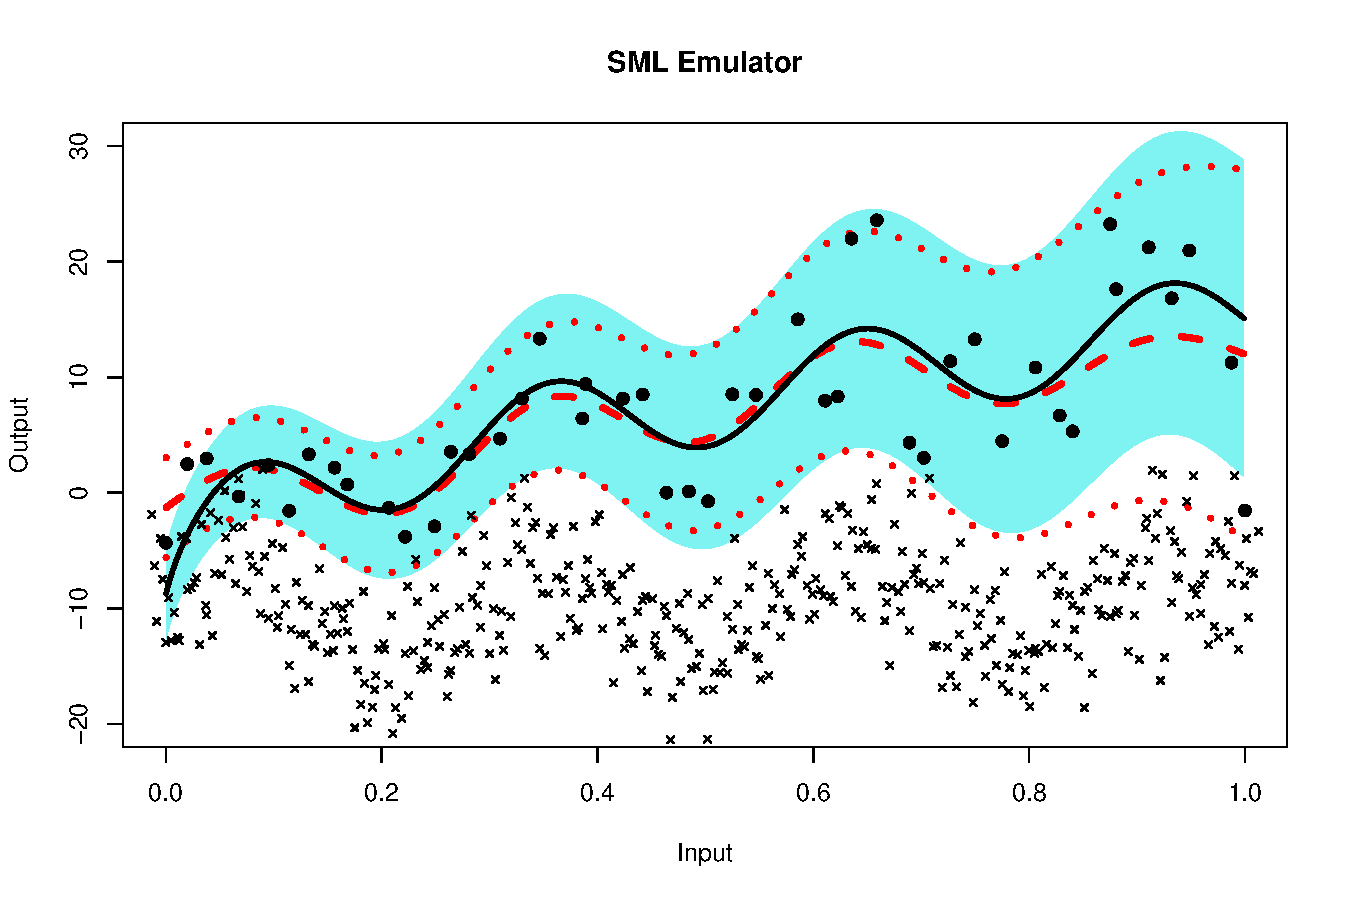
\includegraphics[width=\textwidth]{sml-het-fig2/toy-sml.pdf}
	\caption{A SML emulator for $y(\cdot)$. Expensive runs are black points and cheap runs are black crosses (which are offset by $-10$ to aid visualisation). The true simulator is represented by the black line (mean function) and blue band ($\pm 1.96$ standard deviations). The emulator is represented by the red dashed line (emulator mean) and red dotted lines ($\pm 1.96$ emulator standard deviations).\label{Fig:comparison}}
\end{figure}

\section{Fitting HetGP and SML emulators to Athena \label{sec:fitting}}
As we discussed in the first chapter, one task a subjective Bayesian may want to perform is a probabilistic sensitivity analysis (PSA) to better plan an elicitation exercise. Since Athena is stochastic, we want to understand
\begin{itemize}
	\item[(i)] which parameters influence the mean response
	\item[(ii)] which parameters influence the stochasticity.
\end{itemize}
To perform such a task, with an expensive simulator such as Athena, we first fit an appropriate emulator. HetGP and SML emulators provide what we need here as they provide flexible estimates of both $\E\{y(\bx)\}$ and $\var\{y(\bx)\}$. A key output of Athena is availability, $A(\bx) \in (0,1)$. Since $A(\bx) \in (0,1)$ we will construct emulators for $y(\bx) = \probit \left\{A(\bx)\right\} = \Phi^{-1}\left\{A(\bx)\right\} \in \R$. We will compare a total of $4$ approaches; two estimation routines for fitting HetGP to Athena as well as two estimation routines for fitting SML to Athena.

The first approach will be an \correction{EB} approach; we will integrate out any $\bbeta$ terms in the emulator and find point (MAP) estimates of aspects of the covariance functions. Here we \textit{will not} consider a full-Bayes approach (implemented via MCMC). This is because a full-Bayes approach is incredibly computationally costly due to (a) poor mixing in latent variable models and (b) multiple matrix inversions being required for each iteration of the MCMC scheme \citep{Kersting2007}.

In our second approach, we will fit the emulators via the `full` MAP approach (which can also be thought as a penalised log-likelihood approach). Point estimates are the standard approach to fitting HetGP models and their variants \citep{Binois2019}. MAP estimates can provide improved estimates of lengthscales, as lengthscale parameters can have a very flat likelihood. Comparing MAP estimates to an \correction{EB} approach will also allow us to assess how important uncertainty quantification about the $\bbeta$ parameters is.
\begin{comment}
\section{MAP approach}

The MAP approach estimates $\Theta$ by
\begin{equation}
	\widehat{\Theta} = \argmax_{\Theta} \pi(\Theta \mid \mathcal{D}).
\end{equation}
From a practical perspective, this estimation is performed via \verb|stan| via the \verb|Rstan| interface \citep{stan}.

The posterior distribution of $\log \lambda^2(\bx) \mid \Theta, \log \lambda^2(X)$ is straightforward to compute given estimated values of $\log \lambda^2(X)$. Note that in the MAP approach, we can treat the latent $\log \lambda^2(X)$ as unknown parameters. Thus the \verb|stan| programs used to estimate $\Theta$ also return estimates of $\log \lambda^2(X)$.

Prediction of simulator outputs at inputs $X^*$ first requires the predictive distribution of $\log \lambda^2 (X^*)$.
\begin{equation}
\log \lambda^2(X^*) | \log \lambda^2(X), \mathcal{D}, \Theta \sim \mathcal{N} \left\{ m_V^*(X^*), C_V^*(X^*, X^*) + \lambda_{V}^2 \right\}.
\end{equation}
where the posterior moments are found via the conditional normal equations,
\begin{align}
m^*_V(X^*) & = m_V(X^*) + C_V(X^*, X)
\left[C_V(X, X) + \lambda_{V}^2 I_n \right]^{-1}\left(\log \lambda^2(X) - m_V(X) \right) \\
C_V^*(X^*, X^*) & = C_V(X^*, X^*) - C_V(X^*, X) \left[C_V(X, X) + \lambda_{V}^2 I_n \right]^{-1}C_V(X, X^*)
\end{align}
and $I_n$ is the $n \times n$ identity matrix.
Then conditional on the data, and hyperparameters, the posterior predictive distribution of the simulator at inputs $X^{*}$ is

\begin{equation}
y(\bx^*) | \Theta, \mathcal{D} \sim \mathcal{N} \left\{ m^*(X*) , C^* (X^*, X^*) + \lambda^{2*} (X^*) \right\}.
\end{equation}

Here, $\lambda^{* 2} (X^*) = \exp\{ m_V ^* (X^*) \}$ and $m^*(X^*)$, $C^* (X^*, X^*)$ are also found by the conditional normal equations:

\begin{align}
m^*(X^*) & = m(X^*) + C(X^*, X) \left[ C(X,X) + \lambda^{2 *} (X) I\right]^{-1}\left( \bm{y} - m(\bx) \right) \\
C^*(X^*, X^*) & = C(X^*, X^*) - C(X^*, X) \left[ C(X,X) + \lambda^{2 *} (X) I \right] ^{-1} C(X, X^*) \nonumber
\end{align}

where $\bm{y} = (y_1, \ldots, y_n)$.
\end{comment}
\subsection{Emulator construction}
\label{sec:em-con}

We construct emulators over a $9$ dimensional input space. The input spaces consists of the mean time to degradation (start of phase (3)) of a Bathtub hazard function for the $9$ sub-assemblies in the wind farm. Recall that the $9$ sub-assemblies as follows: 1. gearbox, 2. generator, 3. frequency converter (freq. conv.), 4. transformer, 5. main shaft bearing (MSB), 6. blades, 7. tower, 8. foundations, and 9. catch all. We vary each input over the range $[0.1, 5]$ (years). The Athena simulator is flexible enough to specify unique parameters for every subassembly in every turbine. We give the same parameter values to each subassembly of a given type and allow different types of subassembly to have different parameters. For example, all gearboxes could have a mean time to degradation of $1$ year whereas all generators could have a mean time to degradation of $3.2$ years.

Design points are chosen via the structure described in \Cref{Sec:design}. To construct the HetGP emulator we ran the Athena simulator at $100$ design points. The cheap runs of the simulator were fast enough that we could trade just $5$ expensive design points for $295$ cheap runs. We used basis functions $h(\bx) = (1, \log(\bx))$ for the mean functions of the mean response. We arrived at this selection to reflect a prior belief that the mean availability would flatten off at larger values of $x_i$. The covariance function assumes standardised inputs, $x_i^*$. Standardisation is achieved by subtracting the sample means and then dividing by the sample standard deviations (of the expensive training data). The latent variance GP has mean function $m_V(\bx) = (1, \bx)\bm{\bbeta}_V$ and again, the covariance function assumes standardised inputs.
\begin{figure}
	\centering
	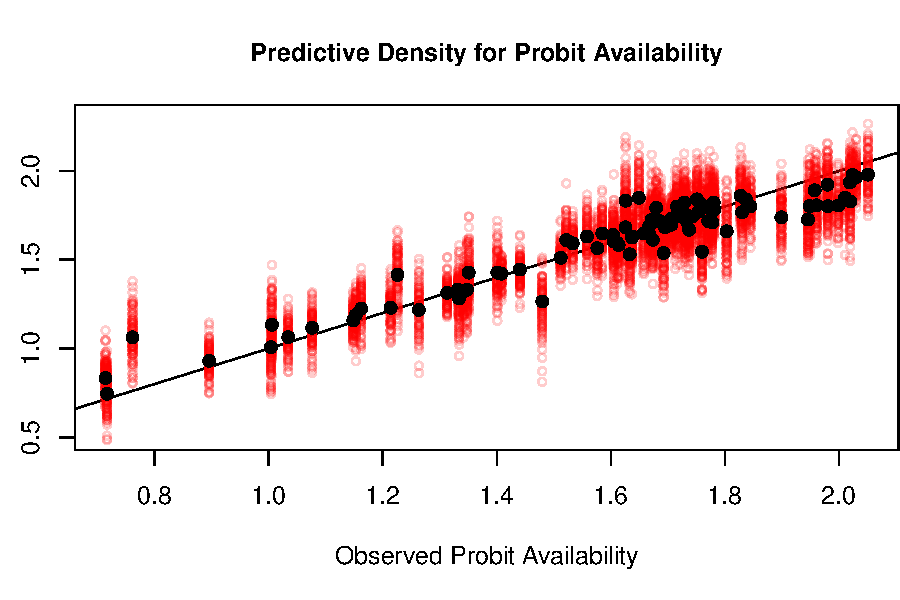
\includegraphics[width=0.7\textwidth]{sml-het-fig2/obs-pred-new.pdf}
\caption{SML emulator mean predictions plotted against observed probit availability (training data from expensive runs of Athena; black dots) and $100$ realisations from the emulator at each point (translucent red circles).\label{Fig:within-sample}}
\end{figure}
\Cref{Fig:within-sample} shows the emulator predictions of the training data (probit scale) with realisations from $\mathcal{N}\{m^{*}(\bx), v^{*}(\bx)\}$ around each prediction. Large deviations from the unit diagonal are typically accompanied by a more diffuse predictive distribution; the emulator is giving larger variance to the points which are far away from the mean. We also see that the observed probit availabilities are mostly in the region of $0.5$ -- $2$ (availabilities in the region of around $0.76$ -- $0.98$). The full range of observed availabilities is $(0.762, 0.980)$; the vast majority of realisations from the emulator agree with this range.

\subsection{Emulator performance comparison}

To judge relative performance of each emulator we use the performance metrics outlined in the previous chapter; RMSE and Score (Equations \ref{Eq:rmse} and \ref{Eq:scoring-rule}). Using $100$ independently generated validation data points, the RMSE (on the probit scale) for HetGP was $0.181$, whereas SML achieved an RMSE of $0.156$. The score for HetGP was $238$ and for SML the score was $254$ (probit scale). Since we transformed the availability to construct emulators on an unbounded space, we should also check how predictions perform on the $[0,1]$ scale. Using an inverse-probit transformation on the mean function provides a sensible point estimate of availability. Comparing the RMSE on the original scale we observe an RMSE of $0.0272$ for HetGP, and under SML this is reduced to $0.0198$. Hence, SML achieves better RMSE and score here than HetGP for the Athena model, suggesting it is a better emulator. Further, our point estimate of $\rho$ is $\hat{\rho} = 0.51$. This suggests a moderate correlation between the two versions of Athena. The additional information extracted from cheap simulations has improved our emulation with little computational cost. It took $5.7$ seconds to fit HetGP and $29.6$ seconds to fit SML on a laptop with $4 \times 2.40\,\text{GHz}$ processors and $8\,\text{GB}$ RAM. Although SML took more time to fit, in real terms this is about $30$ seconds of computation time --- less than a single expensive run of Athena. Both timings are for a total of $3$ fits of the emulator. We performed $3$ fits to prevent using a local maximum being chosen for the point estimates.

\subsection{Emulator validation}

To validate the emulators, we will implement some graphical diagnostics proposed by \citet{Bastos09}. Since we model the (transformed) simulator outputs by a Gaussian process, the Cholesky errors (CEs) should form a random sample from a $\mathcal{N}(0, 1)$ distribution (approximately). If the posterior mean and variance are well suited to the simulator, the validation data should lie in a horizontal band, centred at $0$, with approximately $95\%$ of points in the interval $(-1.96, 1.96)$. We also compare empirical quantiles of the CEs against theoretical quantiles --- we do this via coverage plots which compare the proportion of CEs in the $100(1-\alpha)\%$ prediction interval against the expected proportion.
\begin{figure}[!ht]
  \centering
    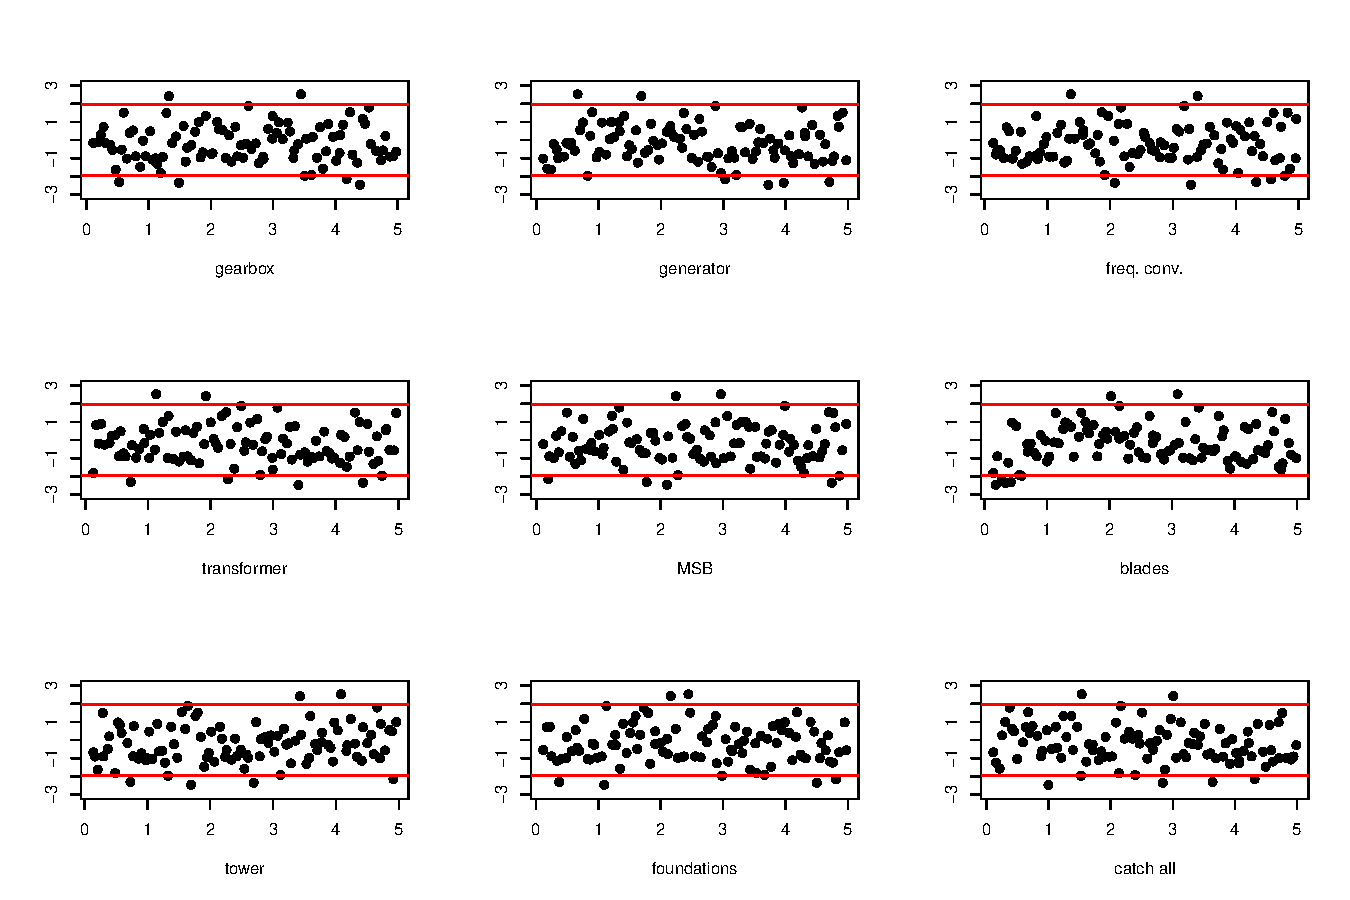
\includegraphics[width = 0.8\textwidth]{sml-het-fig2/het-resids-new3.pdf}
    \caption{Cholesky errors for HetGP, based on $100$ ``unseen'' validation points. Orange lines are at $\pm 1.96$.\label{Fig:het-resids}}
\end{figure}
\begin{figure}[!ht]
  \centering
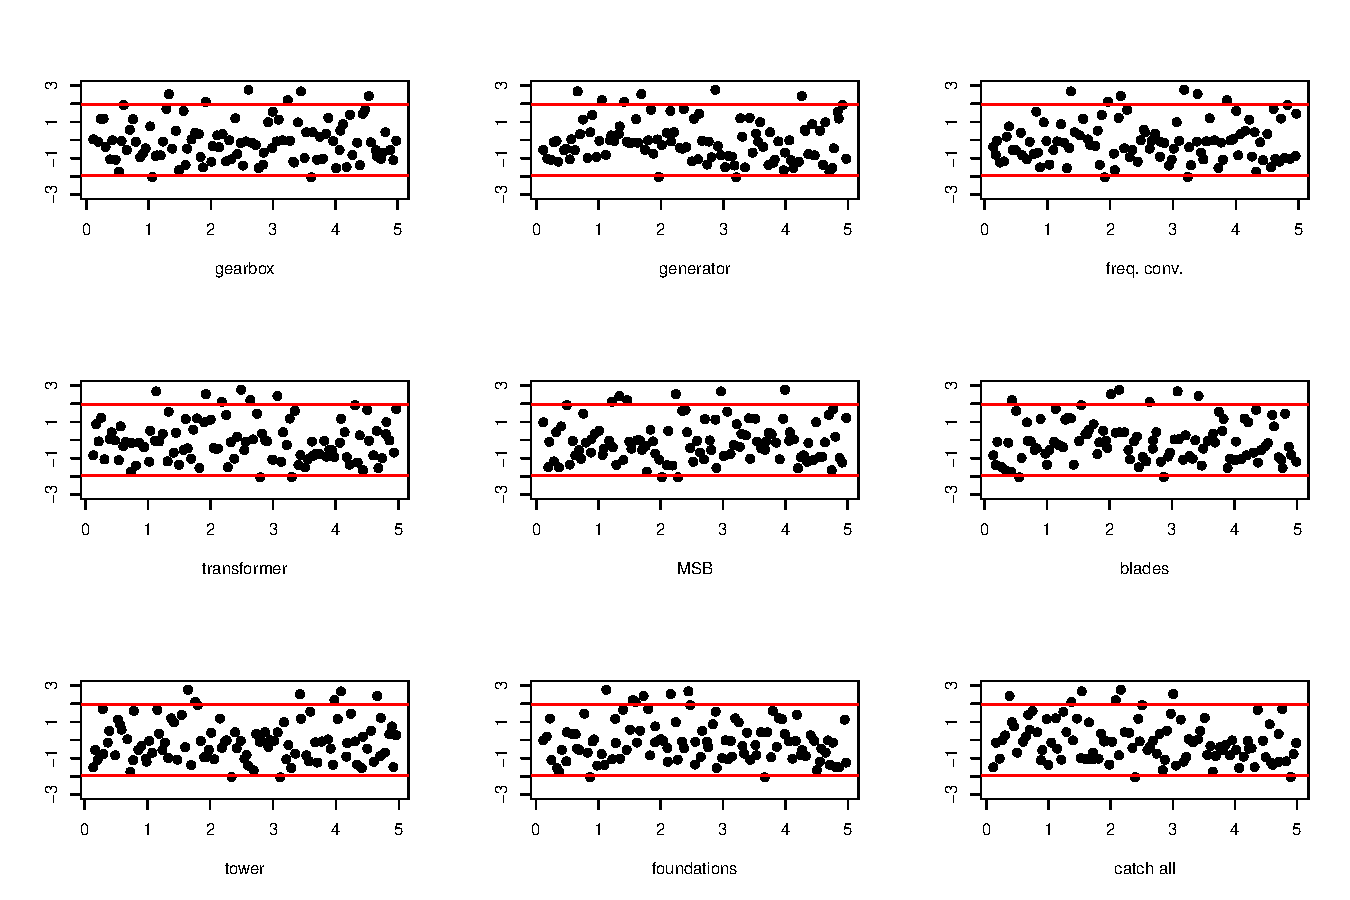
\includegraphics[width = 0.8\textwidth]{sml-het-fig2/sml-resids-new3.pdf}
\caption{Cholesky errors for SML emulation, based on $100$ ``unseen'' validation points. Orange lines are at $\pm 1.96$.\label{Fig:sml-resids}}
\end{figure}
\begin{figure}[!ht]
  \centering
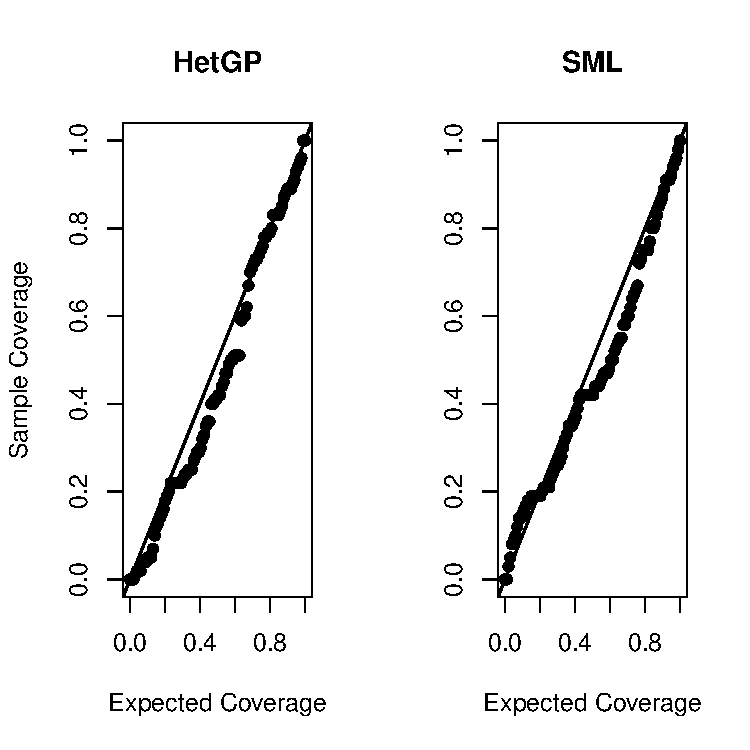
\includegraphics[width = 0.7\textwidth]{sml-het-fig2/coverage-new3.pdf}
  \caption{Out of sample coverage plots (black dots), using the Cholesky errors of the ``unseen'' validation data. Black lines represent the unit diagonal. \label{Fig:coverage}}
\end{figure}
In Figure~\ref{Fig:het-resids} the CEs for HetGP have a distinct pattern when plotted against $x_6$, whereas for SML in Figure~\ref{Fig:sml-resids} the points appear to be closer to a random $\mathcal{N}(0,1)$ sample. The coverage plots in Figure~\ref{Fig:coverage} suggest that for both emulators the coverage is reasonably well calibrated.

\section{MAP approach}

This chapter so far has taken a Bayesian approach to HetGP and SML. Although not fully Bayesian, it takes into account some parameter uncertainty without the often large computational cost of MCMC. In the Athena example, the Bayesian SML emulator provides an accurate and efficient approach to emulation. Although the Bayesian HetGP was not adequate for this example, it was very fast to fit thus could provide useful, and more interpretable, emulators for other stochastic simulators.

However, the majority of the literature uses a MAP/MLE approach to estimate GP hyperparameters and for prediction of simulator output \citep{Binois2018, Baker2020c,Baker2020a, Baker2022, Zhang2022}. Since this is a mathematically simpler approach, which does not rely on specific forms of prior specification, we will investigate whether using the MAP estimate offers improved emulator accuracy and/or improves the computational properties of the emulator.

\subsection{MAP-HetGP prediction}

With the MAP approach, \emph{all} parameters are estimated by their posterior mode. Therefore we will re-define $\Theta := \{\Theta, \bbeta, \bbeta_V \}$. Given $\{\mathcal{D}, \Theta \}$, prediction follows in a similar way to the Bayesian approach.

As in the Bayesian approach, we first predict $\log \lambda^2 (X^*)$. The predictive distribution of $\log \lambda^2 (X^*) \mid \widehat{\Theta}, \log \hat{\lambda}^2(X), \mathcal{D}$ is given by
\begin{equation}
	\log \lambda^2 (X^*) \mid \widehat{\Theta}, \log \hat{\lambda}^2(X), \mathcal{D} \sim \mathcal{N} \{ m_V^*(X^*), v_V^*(X^*) \}
\end{equation}
where the posterior moments are
\begin{align}
	m_V^*(X^*) &= H_V^* \hat{\bbeta}_V + C_V(X^*, X)\left\{ C_V(X, X) + \hat{\lambda}^2_V I \right\}^{-1} ( \log \hat{\lambda}^2 (X) - H_V \hat{\bbeta}_V ) \\
	v_V^*(X^*) &= C_V(X^*, X^*) - C_V(X^*, X)\left\{ C_V(X, X) + \hat{\lambda}^2_V I \right\}^{-1} C_V(X, X^*) + \hat{\lambda}^2_V I.
\end{align}
As with the Bayesian approach, there are three plug-in estimates of $\lambda^2(X^*)$ that can be used. For simplicity, we take $\hat{\lambda}^2(X^*) = \exp\{ m_V^*(X^*) \}$. With this estimate, we can then write the predictive distribution of $y(X^*)$ as
\begin{equation}
	y(X^*) \mid \hat{\Theta},\hat{\lambda}^2(X), \mathcal{D} \sim \mathcal{N} \{ m^*(X^*), v^*(X^*) \}
\end{equation}
where the posterior moments are
\begin{align}
	m^*(X^*) &= H^* \hat{\bbeta} + C(X^*, X)\left\{ C(X, X) + \hat{\lambda}^2(X) I \right\}^{-1} ( y(X) - H \hat{\bbeta} ) \\
	v^*(X^*) &= C(X^*, X^*) - C(X^*, X)\left\{ C_V(X, X) + \hat{\lambda}^2 I \right\}^{-1} C(X, X^*) + \hat{\lambda}^2(X^*) I.
\end{align}
Note that these predictive equations are the same as those derived for the \correction{EB} approach with $B = 0$, $B_V = 0$, $\bm{b} = \hat{\bbeta}$ and $\bm{b}_V = \hat{\bbeta}_V$.
\subsection{MAP-SML prediction}

Much like MAP-HetGP, MAP-SML prediction is obtained by taking the Bayesian version of the predictive equations but setting prior variance matrices to zero matrices and the regression coefficients to their MAP estimates. The design is independent of the statistical paradigm thus we use exactly the same design as above. Since the predictive equations are a direct consequence of the multivariate Normal equations, we present them without proof.

As usual, we start with prediction of the log variance; $\log \lambda^2_E(X^*) \mid \Theta$ is multivariate normal with the following first two moments
\begin{align}
	m_V^*(X^*) &= H_V^* \hat{\bbeta}_V + C_V(X^*, X) \left\{C_V(X, X) + \hat{\lambda}_V^2 I \right\}^{-1} (\log \hat{\lambda}^2 (X) - H_V\hat{\bbeta}_V) \\
	v_V^*(X^*) &= C_V(X^*, X^*) - C_V(X^*, X) \left\{C_V(X, X) + \hat{\lambda}_V^2 I \right\}^{-1} C_V(X, X^*) + \hat{\lambda}^2_V I.
\end{align}
The quantity of interest, $y^E(X^*)$, is also multivariate Normal, conditional on $\Theta, \lambda^2_E(X)$ and $\lambda_E^2(X^*)$ with mean and variance
\begin{align}
	m_E^*(X^*) &= H_V^* \hat{\bbeta}_V +C_0(X^*) \var(\bm{Y} \mid \Theta)^{-1} (\log \hat{\lambda}^2 (X) - H_V\hat{\bbeta}_V) \\
	v_E^*(X^*) &= C_0(X^*, X^*) - C_0(X^*, X) \left\{C_0(X, X) + \hat{\lambda}_V^2 I \right\}^{-1} C_0(X, X^*) + \hat{\lambda}^2_E(X^*)I
\end{align}
where $C_0(X', X) = \cov(y^E(X'), y^E(X)) = \hat{\rho}^2C_C(X', X) + C_E(X, X')$.
\subsection{Performance of MAP estimation}
The advantage of MAP estimation is that it is simpler and, if the user desired, a suitably diffuse prior would return an approximate maximum likelihood estimate. Ultimately, we want to know which performs best for our Athena example. Using the same priors as the Bayesian approach to produce a MAP estimate, we refit the emulators and re-compute out of sample performance metrics using exactly the same validation data as before.
%% go back to KW comments from here
The performance of the MAP-based, and Bayesian, emulators are summarised in \Cref{Tab:all-performance}. All metrics in this table indicate that the Bayesian SML emulator is the best approximation to the Athena simulator. The Bayesian SML emulator does not have the fastest estimation routine, the Bayesian HetGP is fastest. However, this computation time is trivial relative to the computational cost of uncertainty analysis in a computationally expensive simulator such as Athena. The MAP-SML emulator has comparable performance to the Bayesian HetGP emulator in terms of RMSE (probit scale) and score, but the RMSE ($(0,1)$ scale) is quite large. The MAP-SML emulator took a relatively long time to fit and will be slower to implement due to the larger design matrix. The MAP-HetGP offers a marginally better RMSE than its Bayesian equivalent, however the uncertainty quantification under the MAP approach is poor. The score is only $136$ (the Bayesian version had a score or $238$), this poor performance is exemplified by the C.E.s of the Map-HetGP which have a range of $(-3.85, 4.33)$. This stresses that incorporating parameter uncertainty into predictions, especially when the sample size is small, is a wise idea. The Bayesian estimation was much faster than the MAP estimates, this is because the number of parameters to be estimated is much larger in the MAP approach. Assuming each regression function has $p$ inputs and each covariance function has $k$ inputs, the number of parameters for HetGP is $2p + 2k + 3$. For SML there are $3p + 3k + 6$. In our example this equates to $41$ parameters for HetGP and $63$ for SML. The Bayesian approach removes the $p$ terms from each number of parameters; this reduces the dimension of the parameter space to $21$ for HetGP and $33$ for SML.
\begin{table}
	\centering
	\begin{tabular}{lrrrr}
		\toprule
		& \multicolumn{2}{c}{MAP} & \multicolumn{2}{c}{Bayes}\\
		Metric & HetGP & SML & HetGP & SML \\ \cmidrule{1-5}
		Time to fit emulator/seconds &$37$&$307$&$\bm{6}$&$30$\\
		RMSE (probit scale)& $0.179$ & $0.171$&$0.181$&$\bm{0.156}$\\
		RMSE ($(0,1)$ scale) &$0.0248$&$0.0231$&$0.0272$&$\bm{0.0198}$\\
		Score &$136$&$248$&$238$&$\bm{254}$\\\bottomrule
	\end{tabular}
	\caption{Performance summaries for the emulators based on both the MAP and Bayesian versions of the HetGP and SML emulators. Time here denotes the time take for a total of 3 runs of each estimation routine. RMSE and score are correct to $3$ s.f., time is correct to the nearest second. For each row, the bold typeface indicates the best value (largest score is best, for all others, smaller is better).}
	\label{Tab:all-performance}
\end{table}
\section{Summary}
We have reviewed some approaches to emulating stochastic computer models which exhibit input dependent noise. We began with approaches which emulate the mean and variance as separate components and then moved to a single, but more complex, emulator approach. We illustrated that HetGPs can suffer from poor predictive performance in the low-data regime, which is unfortunate since emulators are typically constructed when data (simulator runs) are expensive to obtain. We offered a solution to this by adapting the autoregressive model from \citet{Kennedy2000}.

We have introduced a stochastic multilevel emulator, which adopted elements of (i) the autoregressive structure from \cite{Kennedy2000} to construct a more accurate mean function and (ii) the latent variance structure of HetGP \citep{Goldberg1998, Binois2018} to account for the heteroscedastic nature of the Athena simulator. This structure allowed us to link together two versions of the Athena simulator to construct an emulator with improved accuracy in terms of RMSE and also in terms of score. The easy to generate training data allowed us to build an adequate emulator without relying on a large computational budget to generate training data.

It would be interesting to see, from a methodological point of view, how the SML emulator could be improved. One idea would be to implement a sequential design rule similar to that of \citet{Gratiet2015}, that is, minimising some design criterion such as integrated mean squared prediction error. Another idea would be to use a preliminary round of simulations to see where cheap simulations might be most beneficial. For example, it may be advantageous to place more cheap points where the two levels agree most and then retain the expensive simulation budget for areas where the two levels disagree. It would also be interesting to see if replicates could improve this type of emulator in the same way that replicates benefit HetGP. Replication could be especially beneficial in the cheap simulator; this would help to reduce the size of computational overheads of a large design matrix, since inference is $\mathcal{O}(N^3)$ for HetGP and $\mathcal{O}\left((N_C+N_E)^3\right)$ for SML, however \cref{Tab:all-performance} showed that the raw computation times for the Athena simulator were not particularly large. Prediction is $\mathcal{O}\left(N^2\right)$ for HetGP and $\mathcal{O}\left((N_C+N_E)^2\right)$ for SML. Another possibility would be to link the variance of the two simulators; we chose not to do this as it would involve linking two latent variance processes and would involve inversion of a large matrix, increasing the computational cost of inference and prediction.

A joint emulator is not the only way to use knowledge of cheap simulations to enhance emulation of an expensive simulator. Using a large number of cheap simulations, we can construct an emulator for $y^C(\cdot)$. The joint posterior over the GP hyperparameters and the $\bbeta$ coefficients can be used to construct an informative prior for $y^E(\cdot)$. This could be more computationally efficient than the SML emulator, but would likely require more human input. The informative prior would then be used as part of a HetGP emulator for $y^E(\cdot)$. \citet{Cumming2010} use a large number of runs from a cheap, deterministic simulator to build an informative prior for an expensive, deterministic simulator. Their idea could be adapted to the stochastic, heteroscedastic case in the following way: first use the two-emulator approach of \citet{Henderson09} to obtain an emulator for $y^C(\cdot)$. Next use the MCMC samples obtained from $\pi(\Theta_C \mid \mathcal{D})$ where $\Theta_C$ are the hyperparameters of the GP fitted to $y^C(\cdot)$ to obtain $\pi(\Theta_E)$, the prior for the hyperparameters of $y^E (\cdot)$. Finally, use $\pi(\Theta_E)$ to fit an emulator to $y^E (\cdot)$. We provide no specific details of how to perform such an elicitation, but when constructing $\pi(\Theta_E)$ the analyst should consider how they think the versions of the simulator differ, rather than just setting $\pi(\Theta_E) = \pi(\Theta_C \mid \mathcal{D})$. \citet{Cumming2010} give advice on how to do this within a Bayes linear framework; much of their approach could be applied to a Full Bayesian approach but are particularly relevant to our \correction{EB} approach since both methods focus on uncertainty about regression parameters.

\end{chapter}

  \usetikzlibrary{arrows.meta,
                chains,
                positioning,
                quotes,
                shapes.geometric}

\tikzset{FlowChart/.style={% this style can be used also at other flowcharts,
                           % just call it with "FlowChart", see picture code below
startstop/.style = {rectangle, rounded corners, draw, fill=red!30,
                    minimum width=3cm, minimum height=1cm, align=center,
                    on chain, join=by arrow},
  process/.style = {rectangle, draw, fill=orange!30,
                    text width=5cm, minimum height=1cm, align=center,
                    on chain, join=by arrow},
 decision/.style = {diamond, aspect=1.5, draw, fill=green!30,
                    minimum width=3cm, minimum height=1cm, align=center,
                    on chain, join=by arrow},
       io/.style = {trapezium, trapezium stretches body,   % not used in your flowchart
                    trapezium left angle=70, trapezium right angle=110,
                    draw, fill=blue!30,
                    minimum width=3cm, minimum height=1cm,
                    text width =\pgfkeysvalueof{/pgf/minimum width}-2*\pgfkeysvalueof{/pgf/inner xsep},
                    align=center,
                    on chain, join=by arrow},
    arrow/.style = {thick,-Triangle}
                        }
        }% end of tikzset
% --------------------------------------------------------------
\begin{chapter}{Global Sensitivity Analysis for Stochastic Simulators\label{Ch:sensitivity}}
\section{Introduction}
A simulator used to make statements about a real-world system needs realistic parameter settings. Some parameter values have little uncertainty about them. It is well understood that, close to the earth's surface, acceleration due to gravity takes the value $g = 9.81ms^{-2}$. For complex engineering projects implementing new technologies, the values parameters should take may not be well understood.

In the wind farm setting, consider the lifetime of a gearbox. We may have some understanding of the gearbox lifetime from laboratory testing, such as step accelerated life testing \citep{Nelson1980}. This testing will have been performed under laboratory conditions which offer an imperfect replication of real-world conditions. Although the test will provide a useful indication of the lifetime of a gearbox, there will be marked differences between the test environment and real-world conditions. Alternatively, we may be using old technologies in new environments, and so there will exist historical data from which quantities of interest can be inferred under a different set of conditions to the planned use case. For example, we may be employing onshore technology in an offshore environment, or pushing offshore technology much further away from the shore into deeper waters. In either case, we may have a good understanding of how the technology works in a limited range of conditions. There are intricacies to every problem which need to be considered; for example, the location of the wind farm will have an impact on gearbox lifetimes. Components used in an onshore wind farm in a mild climate will likely last considerably longer than those used in a harsh, offshore environment. This problem can be expressed as trying to obtain the conditional probability $P(T < t \mid E )$ where $T$ is the lifetime of a component such as a gearbox. The event $E$ denotes all relevant aspects of the wind farm, such as the wind farm topology and details of its location. Since there will never have previously been a wind farm with properties described by $E$, the probability $P(T < t \mid E)$ is difficult to obtain with data. A practical solution to this problem is to elicit probability distributions from experts for uncertain quantities \citep{Syed2020, Wilson2021, Dalal2022}.

This input uncertainty means that, even for deterministic computer simulations, the output is also uncertain. Let us return to the gearbox example. Suppose one aspect of $E$ is that the wind farm will be in operation for $20$ years. If the lifetime distribution was specified, or estimated, to be $T \mid E \sim \mathcal{N}(40, 5^2)$, then it is reasonable to assume that gearbox lifetime will have negligible impact on wind farm performance. Whereas if the lifetime distribution is given by $T \mid E \sim \mathcal{N}(10, 3^2)$, it is likely that many gearboxes will fail during the operation of the wind farm and thus gearbox performance could have serious implications for availability. When there are many uncertain parameters in a black-box simulator, it is not clear which are the main contributors to output uncertainty. In the context of eliciting parameters for a complex simulator this is important. Probability elicitation is a time intensive task; especially when multiple experts are used \citep{Williams2021}. Although elicitation is a time consuming task, it is typically much faster and cheaper than collecting an equivalent sample of data.

If an input is deemed important in the simulator, we should elicit the probability distribution over this parameter carefully. We should consider details such as the shape of the parameter's probability distribution. Less important parameters can be assigned a distribution less rigorously; for example a Normal distribution with an appropriate mean or mode (possibly truncating the distribution to avoid non-physical values) or a uniform distribution with appropriate limits. The least important parameters can be assigned a point mass at a plausible value, or be assigned simple distributions. This essentially follows the SHELF guidelines of spending the most time on the most important parameters; see the ``Many Quantities of Interest'' document from \citet{SHELF4} for an elaboration on this philosophy. An illustration of how an elicitation for forward uncertainty propagation can be assisted by emulators and sensitivity analysis is given in \Cref{Fig:elicitation-flowchart}. The first emulator will typically be constructed with all relevant unknowns in mind, whereas the emulator constructed in light of refined uncertainty may be a simpler emulator. In particular, it may be appropriate to construct the emulator over only the more important variables and either condition on a plausible value for unimportant parameters or, if unimportant variables are varied in an experiment, they can be accounted for via the nugget term.
\begin{figure}

\begin{center}
\resizebox{0.4\textwidth}{!}{
\begin{tikzpicture}[FlowChart,                   % used are styles from tikzset FlowChart
    node distance = 5mm and 7mm,
      start chain = A going below                    % The nodes in the chain
                                                     % will be named by A-1, A-2, ...
                        ]
\node   [process] {Identify uncertain model parameters};               % A-1
\node   [process]   {Identify Experts}; %A-2
\node   [process]   {Perform initial elicitation. Identify a simple, but appropriate, distribution for each parameter.};%A-3
\node   [process]   {Construct emulator.};%A-4
\node   [decision] {Adequate emulator?};%A-5
\node   [process]   {Use sensitivity analysis to identify key inputs.};%A-6
\node   [process]   {Revise the elicitation. Give most attention to the most important inputs.};%A-7
\node   [process]   {Reconstruct emulator in light of refined uncertainty.};%A-8
\node   [decision] {Adequate emulator?};%A-9
\node   [process]   {Compute quanitites of interest.};%A-10
% lines not considered by join macro
\draw [arrow] (A-5.west) to ["no"] ++ (-1.5,0) |- (A-4);
\path   (A-5) to ["yes"] (A-6);
\draw [arrow] (A-9.west) to ["no"] ++ (-1.5,0) |- (A-8);
\path   (A-9) to ["yes"] (A-10);
    \end{tikzpicture}
}
\end{center}

\caption{Illustration of how emulators and sensitivity analysis can be used to assist the elicitation for forward uncertainty propagation.}
\label{Fig:elicitation-flowchart}
\end{figure}

The above discussion is well characterised by the following three questions about output uncertainty induced by input uncertainty in a complex simulator:
\begin{itemize}
    \item[1.] If $\bx$ is uncertain; what is the associated uncertainty about $y(\bx)$?
    \item[2.] If $\bx$ is a vector of uncertain inputs, which elements of $\bx$ are contributing the most uncertainty to $y(\bx)$?
    \item[3.] If $y(\cdot)$ is a stochastic simulator, how much output uncertainty is coming from the inherent stochasticity of $y(\cdot)$? How much output uncertainty stems from uncertainty about $\bx$?
\end{itemize}

We will now briefly review some approaches to understanding the impact of uncertain inputs to a simulation model.

\section{Approaches to understanding input uncertainty}

\subsection{Scenario analysis}

A basic approach to considering the impact of input uncertainty is a scenario analysis \citep{Zhang2012, Grewal2013}. The goal of scenario analysis is to make statements of the form \textit{``If we assume $\bx$ happens then $y(\bx)$ will happen''}.

A scenario analysis takes a finite collection of inputs $\mathcal{X}_0 = \{ \bx_1, \bx_2, \ldots, \bx_n\}$  and compares their outputs; $y(\bx_1)$, $y(\bx_2)$, \ldots, $y(\bx_n)$. The set $\mathcal{X}_0$ might be chosen as the sets of inputs corresponding to a desirable scenario, an undesirable scenario and an intermediate scenario. $\mathcal{X}_0$ may also be chosen as a set of moderate inputs and some extreme inputs. If $y(\cdot)$ is stochastic the analyst would analyse the distribution generated by each $\bx_i$. A discussion of scenario analysis is given by \citet{Wheatcroft2019}; they provide details of choosing $\mathcal{X}_0$.

One criticism of this approach is that it is not very exploratory. Scenario analysis only considers a small number of values of $\bx$ and thus we gain a limited understanding of how $\bx$ impacts $y(\bx)$. Even for input vectors of moderate dimension (say $4$), examining the outputs of just a handful of input configurations gives virtually no knowledge of the underlying behaviour of $y(\bx)$.

Another criticism of this approach is that it does not consider how likely each scenario, and hence each $\bx_i$, is; if $y(\bx_1)$ suggests that the wind farm is destined to fail but an expert assessed that $\bx_1$ has negligible density, we might not worry too much about the implications of this scenario.

Although scenario analysis is not well suited to constructed a detailed understanding of complex simulations, it does serve a role in understanding broad, less well defined questions \citep{Criqui2012, Samso2020}.

\subsection{OAT analysis}
One-at-a-time (OAT) analysis aims to generate understanding of $y(\bx)$ (or $f(\bx)$) by varying only the $i$th inputs, $x_i$ over some pre-specified range whilst keeping the remaining inputs, $\bx_{-i}$, fixed at some nominal values. Plotting $f(x_i \mid \bx_{-i})$ allows us to study the influence of $x_i$ on $f(\bx)$ or $y(\bx)$. This type of analysis is very popular outside of the statistical community \citep{Holvoet2005,Khalid2016, Saraiva2017}. OAT analysis is attractive since it is conceptually simple. In varying just one input at a time, we can easily see how $x_i$ impacts the simulator output. There is no noise introduced by varying additional variables (unless $y(\cdot)$ is stochastic). However, a very simple example shows a shortcoming in fixing $\bx_{-i}$ at some nominal value. We argue that this is a naive approach to understanding input importance via the following example.

Consider the following simulator
\begin{equation}
f(x_1, x_2) = x_1 x_2. \label{Eq:oat-simulator}
\end{equation}
\Cref{Eq:oat-simulator} is overly-simplistic and known, but we will imagine it is a black-box. Suppose a modeller conducts an OAT analysis and they choose to vary $x_1$ and $x_2$ over the range $(-1,  1)$. The analyst may then vary $x_1$ over this range whilst fixing $x_2 = 0$, the midpoint of the range. Since $f(x_1, 0) = 0$ for any $x_1$ it appears that $x_1$ has no impact whatsoever on $f(\cdot)$. No simulator of practical interest will be as simple as this, but  \cref{Eq:oat-simulator} displays an important flaw in OAT analysis: an OAT analysis \textit{cannot} detect interactions. Another important criticism of OAT is that, asymptotically, it is a local sensitivity analysis \citep{Saltelli2010}. The argument is constructed by considering the volume of the input space explored compared to the total volume of the input space. Suppose that $\bx \in [0,1]^m$. If we vary inputs individually, we only explore points within the $m$ dimensional hypersphere of radius $\frac{1}{2}$, rather the full hypercube of input configurations. The relative volume of the hypersphere of radius $\frac{1}{2}$ to the unit hypercube is
\begin{equation}
  RV(m) = \frac{\pi^{\frac{m}{2}}}{2^m \Gamma\left(1 + \frac{m}{2}\right)}.
\end{equation}
This expression is fairly complex but, by observing that $\frac{\sqrt{\pi}}{2} < 0.9$ we see that
\begin{equation}
  RV(m) < \frac{0.9^m}{ \Gamma \left(1 + \frac{m}{2}\right) } \to 0 \text{ as } m \to \infty
\end{equation}
since $0.9^m$ is a monotonically decreasing function of $m$, and $\Gamma(1 + \frac{m}{2})$ is monotonically increasing when $m \in [1, \infty)$. The effects of this asymptotic result are felt at small $m$, thus the idea that OAT analysis is `global' is a bit of a myth. For a $9$ dimensional input configuration, like our Athena example from the previous chapter, $RV(9) = 0.0064$. Thus if we were to perform an OAT analysis, we would be exploring less that $1\%$ of the parameter space. $RV(m)$ is plotted in \cref{Fig:relative-volume}. This plot illustrates that, even for problems of small-to-moderate dimension, an OAT analysis is severely under-exploring the input space.  This leads to poor inferences about $f(\cdot)$.
\begin{figure}
  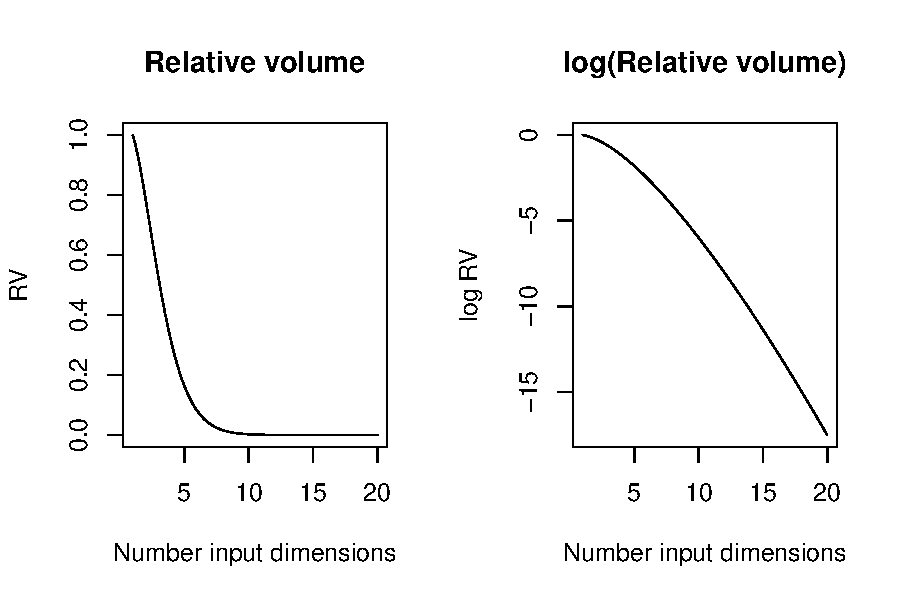
\includegraphics{fig-sensitivity/relative-volume.pdf}
  \caption{Plots showing $RV(m)$ (left) and $\log RV(m)$ (right) for $1 \leq m \leq 20$. Once $m  \geq 10$ the relative volume is essentially $0$. \label{Fig:relative-volume}}
\end{figure}
To consider the full hypercube of input configurations (or a more general shape when inputs are constrained \citep{Kucherenko2017, Kotidis2019}) we need to perform integration. One integration based method is probabilistic sensitivity analysis (PSA). This is frequently called variance based sensitivity analysis and we use the terms interchangeably.
\section{Probabilistic sensitivity analysis for deterministic simulators}
\subsection{Some notation}
Throughout the remainder of this chapter, we will be working with the expectation and variance with respect to
\begin{itemize}
  \item[(i)]  $G(\bx)$ -- the distribution characterising uncertainty about simulator inputs, $\bx$.
  \item[(ii)] $\pi(y(\cdot) \mid \mathcal{D})$ and $\pi(f(\cdot) \mid \mathcal{D})$ -- the posterior distribution of simulator output for stochastic and deterministic simulators respectively.
  \item[(iii)] When $y(\cdot)$ is a stochastic simulator, it will have its own expectation, $\E \{ y(\cdot) \} = f(\cdot) $ and variance $\var \{ y(\cdot) \} = \lambda^2(\cdot)$.
\end{itemize}
To avoid confusion between the expectation and variance induced by $G(\bx)$ and the expectation and variance induced by $\pi(y(\cdot) \mid \mathcal{D})$, we will use $\E_\bx$ and $\var_\bx$ to denote moments with respect to $G(\bx)$. Moments with a $*$ superscript ($\E^{*}$, $\var^{*}$) denote the moments of posterior distributions of simulator outputs. In other words, with respect to $\pi(y(\cdot) \mid \mathcal{D})$ or $\pi(f(\cdot) \mid \mathcal{D})$. We will retain the $m^{*}$  and $v^{*}$ notation used in previous chapters when referring to the posterior mean and variance of $y(\cdot)$. We will use operators without a subscript ($\E$ and $\var$) to denote the ``true'' moments of $y(\cdot)$ and $\log \lambda (\cdot)$.

This section relies on sampling many collections of inputs, $\bx \sim G(\bx)$. We also condition on elements of $\bx$ on many occasions. We will use subscripts, $x_i$, $\bx_J$, to denote elements and sub-vectors of $\bx$. When drawing values of $\bx$ from a (joint) distribution, we will use the notation $\bx^{(j)}$ to denote the $j$th sample of $\bx$.

\subsection{Probabilistic sensitivity analysis}
Within the statistical community, PSA is the go-to method for global sensitivity analysis for two reasons:
\begin{itemize}
  \item[1.] PSA is a global method.
  \item[2.] The output of PSA is straightforward to interpret.
\end{itemize}
One output of PSA is a collection of sensitivity indices (sometimes called Sobol' indices) representing the proportion of uncertainty induced on simulator output by collections of uncertain inputs. The main drawback is that probabilistic sensitivity analysis can be computationally expensive. Thousands of simulator runs are required to obtain reliable estimates of quantities of interest.

When emulators are used in place of a deterministic simulator, $f(\cdot)$, the computational cost is manageable \cite{Becker2012, Overstall2016}. With emulator assisted probabilistic sensitivity analysis, the majority of the computational budget is spent on training an appropriate emulator, which will typically be of the order of a few hundred runs of the simulator. This may be more expensive than a scenario or OAT analysis, but allows for full parameter space exploration and inference about interactions of any order between inputs.

PSA proceeds by specifying a distribution over the inputs $G(\bx)$ and propagating this distribution, and various conditional distributions based on $G(\bx)$, through $f(\bx)$. Sensitivity indices tell us what proportion of the variance in the model output, $V = \var(Y)$, where $Y = f(\bx)$ is the uncertain simulator output, is induced by the uncertainty in (subsets of) inputs $\bx$. First we consider sensitivity analysis for a deterministic simulator and then extend this to the stochastic setting.
\begin{comment}
In the context of probability elicitation, PSA is the go-to method for determining input importance. \citet{Ohagan2012} presented elicitation as a $6$ stage process. In stages $1$--$3$ no probability judgements are elicited. Initial probability judgements are elicited in the $4$th stage. The $5$th stage is revision of beliefs. In this stage, the facilitator shows the experts consequences of their judgements and challenges their beliefs. If this distribution is not compatible with the beliefs of the experts, this suggests that the initial specification should be revised. When a complex simulator is involved, it is usually the case that a small subset of inputs are driving the variability in simulator output(s) \citep{Kennedy2006, Vernon14}. Since the simulator is complex, it is unclear which inputs are driving the outputs. The Sheffield Elicitation Framework (SHELF) approach to expert elicitation advises the elicitation facilitator to spend the largest amount of resources (time and money are two such resources) on the most important parameters. \citet{Ohagan2012} is interested in eliciting parameters of a complex computer model and goes on to perform PSA to determine input importance. The distribution used in the PSA is one obtained from the 4$th$ stage of elicitation. The facilitator should then use the results of PSA to guide stage $5$. In particular, pay most attention to the most
\end{comment}
\subsection{The functional ANOVA decomposition}
PSA relies on the functional ANOVA decomposition. If $\bx$ is a $m$-dimensional input vector then the functional ANOVA decomposition of a function $f(\bx)$ is
\begin{equation}
 f(\bx) = f_0 + \sum_i f_i(x_i) + \sum_{i < j} f_{i,j}(\bx_{i,j}) + \sum_{i<j<k} f_{i,j}(\bx_{i,j,k}) + \ldots + f_{1, 2, \dots, m}(\bx) \label{Eq:functional-anova}
\end{equation}
which is unique when $\bx$ has probabilistically independent components. In \cref{Eq:functional-anova}, $f_0 = \E_\bx(Y)$, and
\begin{equation}
    f_i(x_i) = \E_{\bx_{-i}} (Y \mid x_i ) - f_0
\end{equation}
is the main effect of $x_i$ on $f(\bx)$. The first order interaction effect of $x_i$ and $x_j$ (where $i<j$) is
\begin{equation}
    f_{i,j}(\bx_{i,j}) = \E_{\bx_{-(i,j)}} (Y \mid x_i, x_j ) - f_i(x_i) - f_j(x_j) - f_0.
\end{equation}
This is the effect due to \textit{only} the interaction between $x_i$ and $x_j$, as their main effects are subtracted. Higher order effects for some non-empty subset $J$ of $\{1, 2, \ldots, m\}$ can be extracted from the functional ANOVA decomposition by finding $\E_{\bx_{-J}} (Y \mid \bx_{J} )$ and then subtracting relevant interaction and main effect terms. Plotting $f_i(x_i)$ allows us to understand how $x_i$ influences $f(\bx)$. Likewise, plotting first order effects allows us to understand how pairs of inputs influence $f(\bx)$. This is similar to an OAT analysis but allows for interaction terms and averages over $\bx_{-i}$, rather than conditioning on a single value.
\subsection{Sensitivity indices}
Main effect and interaction plots allow us to gain an intuition of how influential $\bx_J$ is on $f(\bx)$. It is often useful to assign an interpretable value to the relative influence of $\bx_i$ on $f(\bx)$. In PSA, this is achieved by considering the variance of \cref{Eq:functional-anova}.

If $G(\bx) = \prod_i G_i(x_i)$ then taking the variance of both sides of \cref{Eq:functional-anova} leads to
\begin{align}
 \var(Y) &= \sum_{J \subseteq \{1, 2, \ldots, m\} }  \var_{\bx_{J}} \{ f_J(\bx_J) \}\\
         &= \sum_{J \subseteq \{1, 2, \ldots, m\} }  \var_{\bx_{J}}  \{ \E_{\bx_{-J}} [ Y \mid \bx_J ] \}
\end{align}
The above sum has $2^{m} - 1$ terms; one for each non-empty subset of $\{1, 2, \ldots, m \}$.
The first type of sensitivity index is
\begin{align}
    S_i &= \frac{V_i}{V}\\
    V_i & = \var_{x_{i}} \{ \E_{\bx_{-i}} [ y(\bx) \mid X_{i} ] \}.
\end{align}
Here, $S_i$ is the proportion of $\var\{Y\}$ induced by the uncertainty about $x_i$. This tells us that, if we were to learn the `true' value of $x_i$, then we would expect $\var\{Y\}$ to decrease by $100S_i\%$. This can be generalised to any subset $J$;
\begin{equation}
 S_J = \frac{1}{V} \sum_{J' \subseteq J} V_{J'}
\end{equation}
\correction{where $S_J$ is the amount of variability explained by the variables corresponding to $J$.}

The second type of sensitivity index is
\begin{equation}
    S_{T_i} = \frac{V - \var_{x_{-i}} \{ \E_{x_i} (Y \mid \bx_{-i}) \} }{V}
\end{equation}
which represents the proportion of $\var_\bx \{Y\}$ remaining when all inputs apart from $x_i$ have been learnt. \correction{This can be generalised to $S_{T_J}$, which represents the remaining uncertainty when all inputs apart from those corresponding to $J$ have been learnt.} In this chapter we focus mainly on $S_J$ rather than $S_{T_J}$ since we are interested in using sensitivity analysis for probability elicitation. We need to deduce how to reduce uncertainty about $\bx$ in a way which efficiently reduces uncertainty about $Y$, which is what $S_i$ tells us. The $S_i$ and $S_J$ have a natural decision theoretic justification as measures of importance, which we now discuss.
\subsection{Linking PSA to EVPI: decision theoretic justification for $S_i$}
Let $u(a, \bx)$ be a utility function for decision $a \in \mathcal{A}$ when the (random) consequence $\bx$ occurred. Let $U(a) = \E_\bx \{ u(a, \bx) \} $ be the expected utility of decision $a$. Let $U^* = U(a^*)$ where $a^* = \argmax_{a \in \mathcal{A}} U(a)$ is the optimal decision.

In decision theory, EVPI (expected value of perfect information) is the price the decision maker would pay to obtain the precise value of an uncertain quantity $x_i$. The EVPI for input $i$ is given by
\begin{equation}
    \text{EVPI}_i = \E_{x_i} \left\{  \max_{a \in \mathcal{A}} \E_{\bx \mid x_i} u(a, \bx)  \right\} - U^*.
\end{equation}
EVPI is interpreted as the price a decision maker would pay to have access to perfect information; the true value of $x_i$. In our context, `perfect information' is the true value of an uncertain parameter to a simulator. Now suppose our goal is to obtain the true value, or the best possible point estimate, of $f(\bx)$ when $\bx$ itself is uncertain. To define the `best possible' point estimate, a Bayesian would specify a utility function describing how (un)desirable using $a$ as an estimate of $f(\bx)$ is. A commonly used utility function in estimation routines is squared loss. Thus we take our utility function to be
\begin{align}
U(a) &= -\E_{\bx} \{(a - f(\bx))^2\}\\
      &= -a^2 + 2a\E_{\bx} \{ f(\bx) \} + \E_{\bx} \{ f(\bx)^2 \}
\end{align}
which is maximised at $a^{*} = \E_{\bx} \{ f(\bx) \} $, the expected simulator output. Thus the EVPI, under this utility function is,
\begin{align}
\text{EVPI}_i &= \E_{x_i} \{ -\var_{X_{-i}}[ f(\bx) \mid X_i ]  \} - (-)\var_\bx \{ f(\bx) \} \\
              &= \var_{\bx} \{ f(\bx) \} -\E_{X_i} \{ \var_{\bx_{-i}}[ f(\bx) \mid x_i ] \}\\
              &= \var_{x_i} \{ \E_{\bx_{-i}} [ f(\bx) \mid x_i ]  \}\\
              &= V_i.
\end{align}
The sensitivity index $S_i = V_i / V$ improves the interpretability of EVPI; $S_i$ represents the proportion of variation in $f(\bx)$ explained by $x_i$. This relationship between $S_i$ and EVPI tells us that, if $S_k$ is the largest sensitivity index and we are able to learn the precise value of only one input, then we should learn $x_k$. If we can learn two inputs, then we should learn the pair $(k, l)$ which maximise $S_k + S_l + S_{k,l}$. If we want to learn $Q$ inputs, we should learn the set $J$ of size $Q$ which maximises $\sum_{J' \subseteq J} S_J'$.

\subsection{Computation of sensitivity indices}

\citet{Sobol1993} provides Monte Carlo based algorithms for computing sensitivity indices. Many runs are required to compute the indices, which is not problematic for computationally cheap simulators. Slow run times of complex simulators induce a computational bottleneck in PSA. Replacing the simulator by an emulator provides huge computational savings without much loss of accuracy when the simulator is computationally expensive. In the deterministic case, particular forms of $G(\bx)$ lead to a tractable emulator-based PSA \citep{Oakley04}. We will present the more general case via Monte Carlo simulation, which does not rely on the form of emulator or specification of $G(\bx)$. The Monte Carlo case also allows for distributional estimates of $S_J$, whereas \citet{Oakley04} produce only $\E^{*}\{V_J\}$ and $\var^{*}\{V_J\}$.
\subsubsection{Constructing main effects plots}
To begin the analysis we must estimate $f_0$. This is achieved via the usual estimate of the mean;
\begin{align}
f_0 & = \int f(\bx) \,\dd G(\bx) \\
& \approx \frac{1}{N} \sum_{j = 1}^N f (\bx^{(j)}) \\
& =  \hat{f}_0
\end{align}
where $\bx^{(j)} \iid G(\bx)$. Simple i.i.d. sampling returns an \correction{unbiased} estimate for $f_0$. If each $x_i \sim U(a, b)$ then Latin Hypercube sampling offers an estimate that is still unbiased but more efficient \citep{Mckay1979, Stein1987}.

Estimates of main effects are given by
\begin{align}
f_i(x_i) &  = \int f(\bx) \,\dd G(\bx_{-i} \mid x_i ) - f_0\\
	& \approx \frac{1}{N} \sum_{j = 1}^N f(\bx^{(j)} \mid x_i)  - \hat{f}_0. \label{Eq:main-effect-est}
\end{align}
Now, $f_i(x_i)$ is a function; plots of $f_i(x_i)$ are constructed by evaluating \cref{Eq:main-effect-est} over a sequence of values for $x_i$.

Estimation of the functions implied by interaction effects is as follows:
\begin{equation}
\hat{f}_{i,j}(x_{i,j}) = \frac{1}{N} \sum_{k = 1}^N f(\bx^{(k)} \mid x_{i,j})  - \hat{f}_i(x_i) - \hat{f}_j(x_j) - \hat{f}_0. \label{Eq:interaction-plot-est}
\end{equation}

The above estimation procedures assume that we are directly using the simulator. If we are using a GP emulator to facilitate computation then we have posterior distributions for these quantities. The posterior mean of $\hat{f}_i(x_i)$ is obtained by replacing $f(\bx)$ by $m^*(\bx)$ in \cref{Eq:main-effect-est} and \cref{Eq:interaction-plot-est}. The posterior variance can be found by replacing $f(\bx)$ by $v^{*}(\bx)$, and turning subtractions into additions. Monte Carlo estimates can be obtained by drawing random functions from $\pi(f(\cdot) \mid \mathcal{D})$  to produce a probability distribution for $f(x_i)$.

\subsubsection{Estimating sensitivity indices}

To estimate $V$, assuming direct use of the simulator, we can use the standard variance estimate;
\begin{equation}
 \hat{V} = \frac{1}{N-1} \sum_{j=1}^N (f(\bx^{(j)}) - f_0)^2.
\end{equation}

To compute $V_i$ we need to find the variance of an expectation. Some manipulation of expectations gives us a more attractive way forward. Starting from the definition of $V_i$ we have
\begin{align}
V_i &= \var_{x_i} \left\{  \E_{\bx_{-i}} [f(\bx)\mid x_i] \right\}\\
    &= \E_{x_i}\left\{  \E_{\bx_{-i}} [f(\bx)\mid x_i]^2 \right\} - \E_{x_i}\left\{  \E_{\bx_{-i}} [f(\bx)\mid x_i] \right\}^2\\
    &= \E_{x_i}\left\{  \E_{\bx_{-i}} [f(\bx)\mid x_i]^2 \right\} - \E_{\bx} \{ f(\bx) \}^2.
\end{align}
Now a Monte Carlo estimate of $E_{\bx} \{ f(\bx) \}^2$ is straight forward; $(\hat{f}_0)^2$. This will be slightly biased for $\E_{\bx}\{f(\bx)\}^2$, but with sufficiently large $N$, the bias will be negligible. The use of an emulator means obtaining sufficiently large $N$ is not a problem. Estimating $T_i  = \E_{x_i}\left\{  \E_{\bx_{-i}} [f(\bx)\mid x_i]^2 \right\}$ is a bit more of a challenge. An efficient estimation method --- under the assumption that $\bx$ is uniformly distributed on $[0, 1]^m$ is given in Chapter $8$ of \citet{Gramacy2020surrogates}. \correction{We illustrate this algorithm in \cref{alg:est-Si} under the assumption that $G_i(x_i) = \mathcal{U}(0, 1)$.}

\begin{algorithm}[h]
\caption{Point estimation of $S_i$}\label{alg:est-Si}
\begin{algorithmic}
\Require Estimates $\hat{f}_0 \approx \E_\bx \{ f(\bx) \} $, $\hat{V} \approx \var_{\bx} \{ f(\bx) \}$.
\For{$i = 1$, $2$, $\ldots$, $m$}
  \State Construct an $N \times m$  Latin hypercube, $X$
  \State \correction{$\tilde{X} \gets X$}
  \For{$j = 1$, $2$, $\ldots$, $N$}
  \State $\tilde{x}_{i,j} \sim G_i(x_i)$ \Comment{Re-draw the $i$th elements of $\tilde{\bx}_j$}
  \EndFor
  \State $\hat{T}_i \gets \frac{1}{N-1}\sum_{j=1}^N m^{*}(\bx_j)m^{*}(\tilde{\bx}_j)$
  \State $\hat{S}_i \gets \frac{\hat{T}_i - \hat{f}^2_0}{\hat{V}}$
\EndFor
\State Return estimated sensitivity indices $\hat{S}_1$, $\hat{S}_2$, \ldots, $\hat{S}_m$.
\end{algorithmic}
\end{algorithm}
Bayesian estimation is based on having many posterior draws of $f(\cdot)$. If draws are available, then for each draw we execute \cref{alg:est-Si} and return the set of point estimates as a single draw of each value. Many draws are used to approximate the joint posterior distribution of the $S_i$.

It is straightforward to adapt \cref{alg:est-Si} can be adapted to when $\bx$ is not uniformly distributed on $[0,1]^m$ but does have probabilistically independent elements. We replace $G_i(x_i)$ by the distribution of $x_i$ and the $i$th column of $X$ must be $N$ i.i.d. samples from $G_i(x_i)$, this column must also be independent of the other columns.

\correction{The above MC estimates are often relying on one or more previously found MC estimates. The convergence of these `nested' MC schemes (NMC) has been analysed in the machine learning literature. For example, \citet{Rainforth2018} provide optimal convergence rates for NMC schemes. In general, convergence is slower as the number of nested approximations increases. In this work, we only have two levels of nesting (the variance of the mean), and our emulators are sufficiently cheap that achieving negligible bias with a small wall-clock CPU time is achievable.}

\section{Extending PSA to the stochastic case}
The Athena simulator is stochastic so the illustrated methodology needs to be adapted. Re-applying the above methodology to the emulator mean will allow us to perform inference about $\E\{ y(\cdot) \}$. Because the illustrated approach was devised with deterministic simulators in mind it cannot address two important aspects of sensitivity analysis in stochastic simulation:
\begin{itemize}
	\item[1.] Quantifying the amount of output uncertainty induced by the stochastic nature of the simulator.
	\item[2.] Understanding which input variables are driving the stochasticity.
\end{itemize}
Fortunately, \citet{Marrel2012} present an appropriate solution to both the above concerns which places few restrictions on the form of the emulator.  The core requirements are a model for the mean and another for the variance (or other measure of dispersion). Therefore, their approach applies to our HetGP and SML emulators constructed in \cref{Ch:Hetsml}. They compartmentalise the simulator; $y_m(\bx) = \E \{ y(\bx) \} $ is the mean component of the simulator and $\lambda^2(\bx) = y_d(\bx) = \var \{ y(\bx) \} $ is the dispersion component. We will retain our notation from \cref{Ch:Hetsml} using $f(\cdot)$ and $\lambda^2(\cdot)$  to denote the `true' mean and variance of $y(\cdot)$. The approach of \citet{Marrel2012} formulates a stochastic computer model $y(\cdot)$ as a function of $\bx$, the simulator inputs, but also $x_\varepsilon$, the state of the pseudo random number generator of the simulator. Although, in theory, we could `open up' the black box simulation and observe the state of the random number generator, we treat $x_\varepsilon$ as an unknown quantity. We refer to $x_\varepsilon \in \N$ as the ``seed variable''.
\subsection{Determining input importance for $y(\bx)$}
Since $f(\bx) = \E \{ y(\bx) \}$ is a deterministic function, the ANOVA decomposition is precisely the same as \cref{Eq:functional-anova}. In addition, $y(\bx)$ has a similar functional ANOVA decomposition which takes $x_\varepsilon$ into consideration
\begin{equation}
y(\bx) = f(\bx) + f_\varepsilon(\bx) + \sum_{J \subseteq \{1, 2, \ldots, m\}} f_{\varepsilon, J}(\bx) \label{Eq:stoch-anova}
\end{equation}
where $f_\varepsilon(\bx)$ is the main effect of the seed variable and $f_{\varepsilon, J}(\bx)$ represents the interaction term between the seed variable and the subset of variables attributed to the set $J$. As with the deterministic case, $V_J/V$, determines how much uncertainty of the subset of variables $J \subseteq \{1, 2, \ldots, m \}$ contributes to the total variance in $y(\bx)$. However, because $y(\bx)$ is stochastic, the total variance formula tells us that
\begin{align}
V & = \var_{\bx} \{ \E[y(\bx) \mid \bx ] \} + \E_{\bx} \{ \var[y(\bx) \mid \bx] \}\\
  &  = \var_\bx \{ f(\bx) \} + \E_\bx \{ \lambda^2(\bx) \}.
\end{align}
The definition of $V$ has been adjusted to account for stochasticity, therefore,
\begin{equation}
\sum_{J \subseteq \{1, 2, \ldots, m \} } V_J < V.
\end{equation}
The additional variability comes from $x_\varepsilon$. We now have
\begin{equation}
V = \left( \sum_{J \subseteq \{1, 2, \ldots, m \} } V_J \right)+ V_{T_{\varepsilon}}
\end{equation}
with $V_{T_{\varepsilon}}  = V \times S_{T_\varepsilon}$ being the total variance induced by $x_\varepsilon$.
\subsection{Determining input importance for $\log \lambda^2(\bx)$}
Under the HetGP and SML assumptions, $\log \lambda^2(\bx)$ is an arbitrary function. To avoid cumbersome notation, we define $\ell(\bx) = \log \lambda^2 (\bx)$. A functional ANOVA decomposition of $\ell(\bx)$ is also possible. We adopt the convention used in \cref{Ch:Hetsml} and place a $\lambda$ superscript on any quantities related to $\ell(\bx)$. The functional ANOVA decomposition of $\ell(\bx)$ is
\begin{equation}
\ell(\bx) = f^{\lambda}_0 + f^{\lambda}_\varepsilon (\bx) + \sum_{J\subseteq \{ 1, 2, \ldots, m\}} f^{\lambda}_J(\bx) . \label{Eq:lambda-anova}
\end{equation}
There are no interaction terms between $\bx$ and $x_\varepsilon$ in \cref{Eq:lambda-anova} because  $\lambda^2_V$ is assumed constant. It would be possible to construct an ANOVA decomposition of the variance of $\ell(\bx)$, however, this is a fourth order statistic. Emulation of this quantity is discouraged since estimates of fourth order statistics can be highly unstable and it is not clear what the benefits of such an analysis would be \citep{Andrianakis2017}.
Sensitivity indices for $\log \lambda^2(\bx)$ proceed in a similar way to $y(\bx)$. The total variance of $\ell(\bx)$ is given by
\begin{equation}
\var_\bx \{ \ell(\bx)\} = \lambda^2_V + \var_{\bx} \{\correction{ \E [ \ell(\bx) ] }  \}
\end{equation}
where \correction{$\E \{ \ell(\bx) \} $} is the `true' value of $\ell (\bx)$. The $S^{\lambda}_J$ have definitions which follow naturally from $S_J$ and and $S_{T_\varepsilon}$. In the log variance context, $S^{\lambda}_{T_\varepsilon}$ is the amount of uncertainty about $\log \lambda^2(\bx)$ that is present due to the stochasticity of simulations. We can also compute main effects in an analogous way to $y(\bx)$.
\subsection{Computation of sensitivity indices}
We discuss some details of the computation of the sensitivity indices in the stochastic case as well as understanding the importance of $S_{T_\varepsilon}$. We only provide details of point estimates of the quantities of interest; however our results later give posterior distributions for the sensitivity indices. The posterior distributions are obtained by drawing random functions from the emulator and computing a corresponding point estimate for each draw.
Computation of $S_{T_\varepsilon}$ is fairly simple. First we need to estimate $V$. To do this, we use
\begin{equation}
\hat{V} = \widehat{\var}_{\bx} \{ f(\bx) \}  + \bar{\lambda}^2 (\bx)
\end{equation}
where
\begin{align}
\bar{\lambda}^2 (\bx) &  = \frac{1}{N} \sum_{j=1}^N \hat{\lambda}^2(\bx)\\
\widehat{\var}_{\bx} \{ f(\bx) \} \ &= \frac{1}{N-1} \sum_{j=1}^N (m^*(\bx^{(j)}) - \hat{f}_0)^2
\end{align}
and then
\begin{equation}
 \hat{S}_{T_\varepsilon} = \frac{\hat{V} - \widehat{\var}_{\bx} \{ y_m(\bx) \} }{\hat{V}}. \label{eq:steps-hat}
\end{equation}
Introduction of $S_{T_\varepsilon}$ is one of the novel contributions from \citet{Marrel2012}; it is the total proportion of variability attributed to the stochastic nature of $y(\cdot)$. The physical interpretation of $S_{T_\varepsilon}$ is the total sensitivity attributed to all stochastic processes in the simulator. It essentially measures how random a simulator is.
Then estimates of $S_i$ follow directly from estimates of $T_i$, $\E_\bx \{y(\bx) \}$ and $V$ and have the usual interpretation. \citet{Marrel2012} suggest estimating $S_{T_\varepsilon}$ by \cref{eq:steps-hat} to ensure that $S_{T_\varepsilon} + \sum S_J = 1$. We cannot compute $S_\varepsilon$ or any $S_{\varepsilon, J}$; they are non-identifiable because $x_\varepsilon$ is not observed. Thus we have a limited understanding of how important the stochasticity in the simulator is or how the seed interacts with elements of $\bx$.

\section{Application of PSA to the Athena simulator}
We apply the above methodology to the Athena simulator. To facilitate the computation, we use our SML emulator from \cref{Ch:Hetsml} which emulated $\probit \left[ A(\bx) \right]$ for a $9$ dimensional, uncertain input vector $\bx$. The elements of $\bx$ are exactly the same as in the previous chapter. As a reminder, they are the mean time to failure for the 9 sub-assemblies; 1. gearbox, 2. generator, 3. frequency converter (freq. conv.), 4. transformer, 5. main shaft bearing (MSB), 6. blades, 7. tower, 8. foundations, and 9. catch all.

We also revisit the HetGP emulator. We know that the SML emulator improved RMSE and score. The black-box nature of emulators means it is difficult to see \textit{why} one emulator offers a better representation of the simulator. Since main effect plots give an impression of the shape of the simulator we may be able to understand why one emulator has outperformed the other. The results here are also presented in \citet{Kennedy2023}.

Our choice of $G(\bx)$ is given by $x_i \iid \mathcal{U}(0.1, 5)$, which is uniform over the range of inputs our emulators were constructed. This is a useful and practical distribution for PSA when we have limited access to experts \citep{Saisana2005,Overstall2016}. Our estimation approach is Bayesian; we draw $1000$ different functions from the posterior distribution and then for each draw compute Sobol' sensitivity indices based on Latin hypercube samples of size $N=10^4$. Boxplots of first order indices based on both HetGP and SML are given in \Cref{Fig:si-mean}. In both cases, $\sum_{i=1}^9S_i + S_{T_\varepsilon}\approx 1$ suggesting Athena is approximately additive in the inputs. Some realisations of $S_i$ are negative, this is a symptom of Monte Carlo error and happens when $S_i \approx 0$ \citep{Gramacy2020surrogates}. Note that all posterior means and medians of $S_i$ are positive, and the negative draws are usually identified as outliers, indicated by a $\times$ on the boxplots.
\begin{figure}[ht]
   \centering
   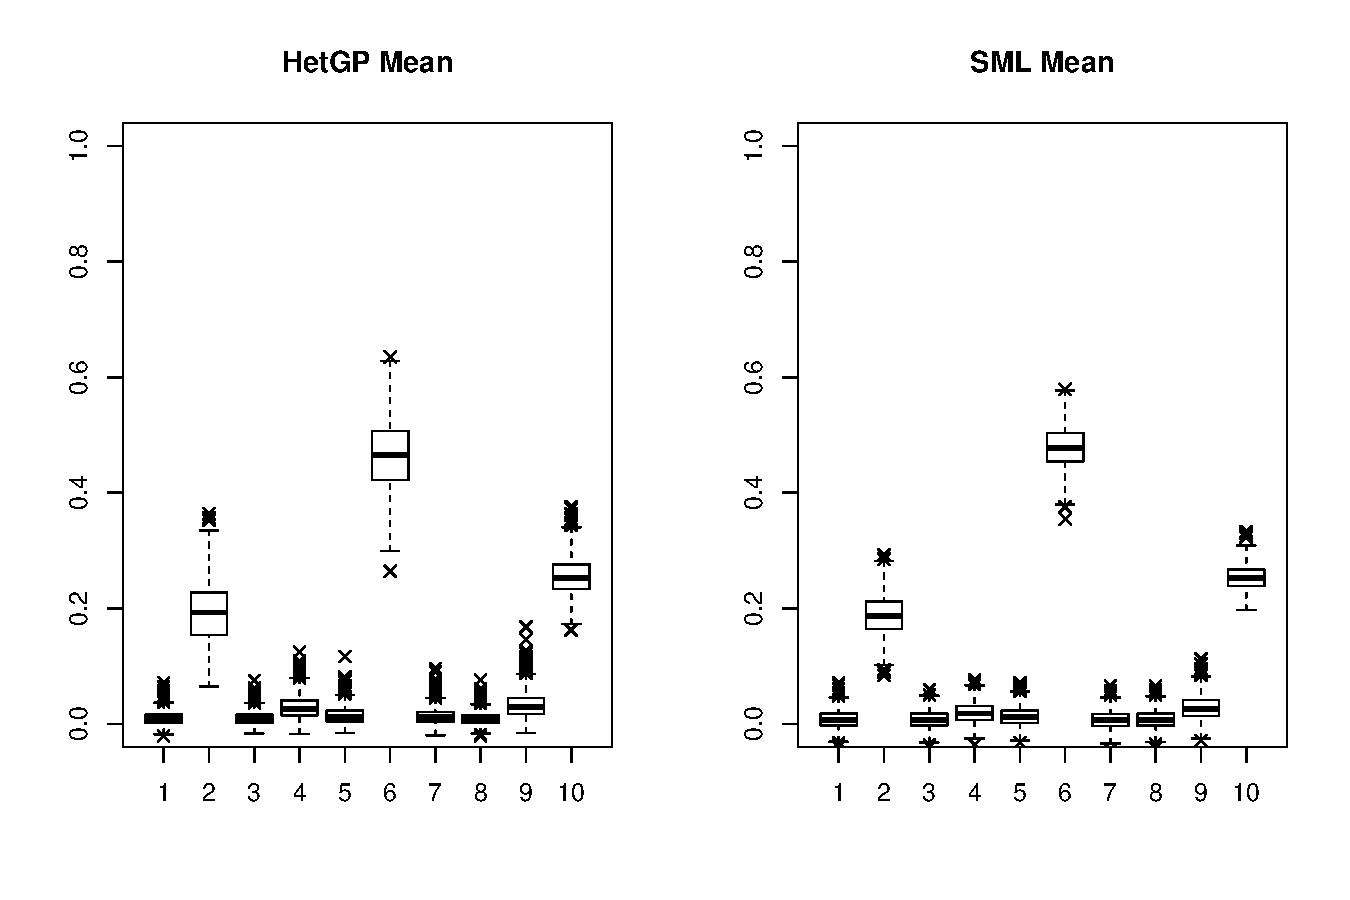
\includegraphics[width=0.9\textwidth]{fig-sensitivity/si-mean4.pdf}
   \caption{Boxplots representing the posterior distribution of $S_i$; $i=1$, $2$, \ldots, $9$. The $10^{th}$ index corresponds to $S_{T_\varepsilon}$. The left hand plot corresponds to HetGP; the right hand to SML.}  \label{Fig:si-mean}
\end{figure}
We should not worry about small differences amongst the $S_i$ since they are functionals of $G(\bx)$, which is a rough approximation to an expert's beliefs. We should focus on larger differences. Estimated first order sensitivity indices for the mean give us more-or-less the same interpretation about the Athena simulator. We see in both cases that $S_6  > S_{T_\varepsilon} > S_2$ are the three most important indices, and the rest have mean values comfortably under $5\%$. Since $S_{T_\varepsilon}$ is clearly larger than all but one first order effect, this suggests the stochasticity in the Athena simulator is an important part of the model (inherent stochasticity contributes to slightly more output uncertainty than $x_2$).
 The most dramatic difference between the approaches is the estimates of $S^{\lambda}_i$ and $f^{\lambda}_i(x_i)$. Observing \Cref{Fig:si-var} we can see that the HetGP estimate of $S^{\lambda}_6$ is very large (around $50\%$) whereas under SML the estimate is less than $10\%$. We suspect that HetGP is interpreting a large proportion of the systematic variation due to $x_6$ as noise, this is because $S_6^{\lambda}$ is estimated to be large via HetGP. SML estimates that $S_6^{\lambda}$ is fairly small and provides a slightly larger estimate of $S_6$ than HetGP.
\begin{figure}[ht]
  \centering
  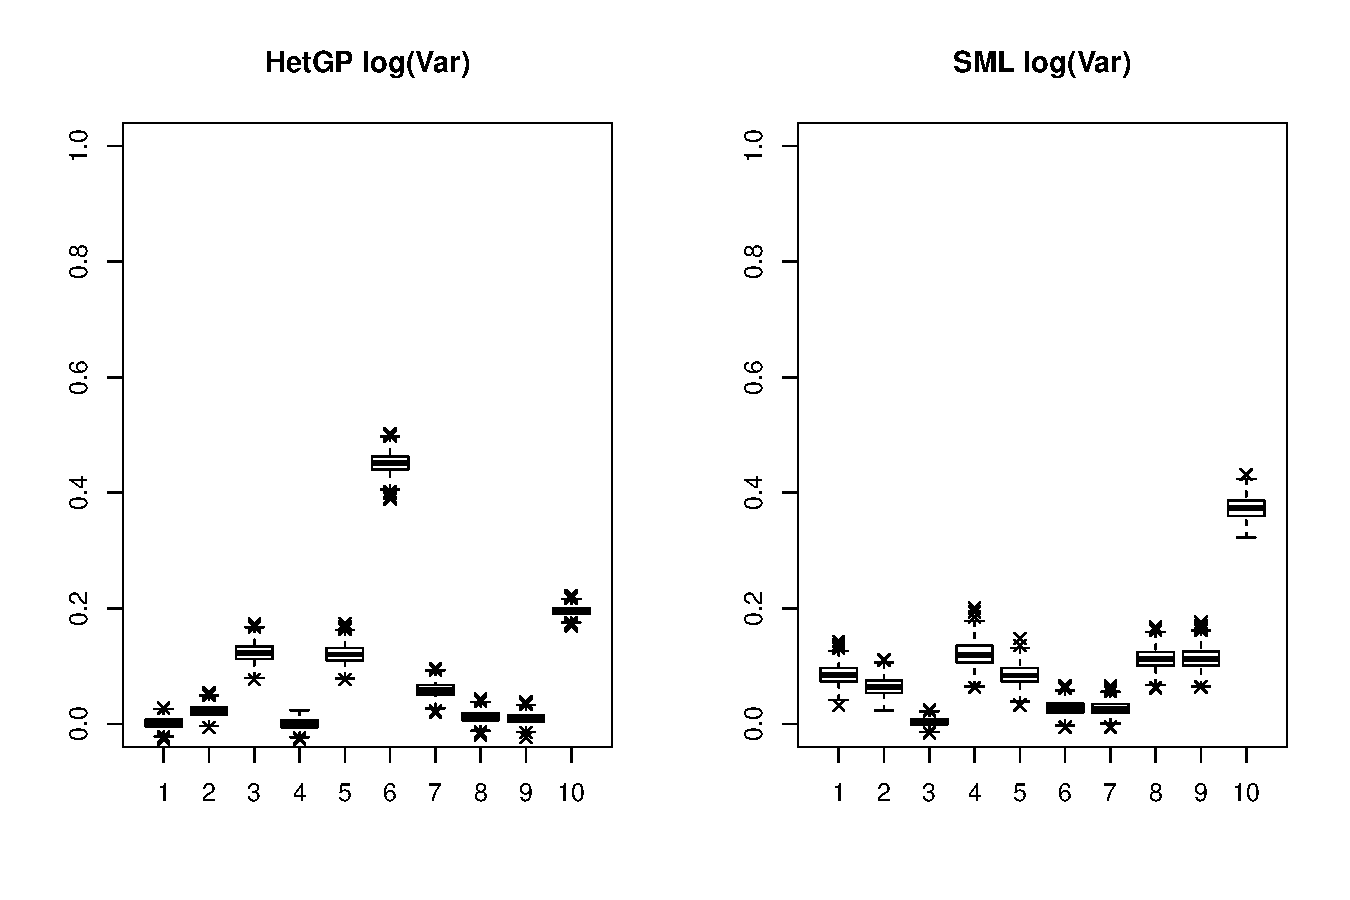
\includegraphics[width=0.9\textwidth]{fig-sensitivity/si-var4.pdf}
  \caption{Boxplots representing the posterior distribution of $S_i^{\lambda}$; $i=1$, $2$, \ldots, $9$. The $10^{th}$ index corresponds to $S_{T_\varepsilon}$. Left hand plot corresponds to HetGP; right hand to SML.}
   \label{Fig:si-var}
\end{figure}
\begin{figure}[ht]
   \centering
   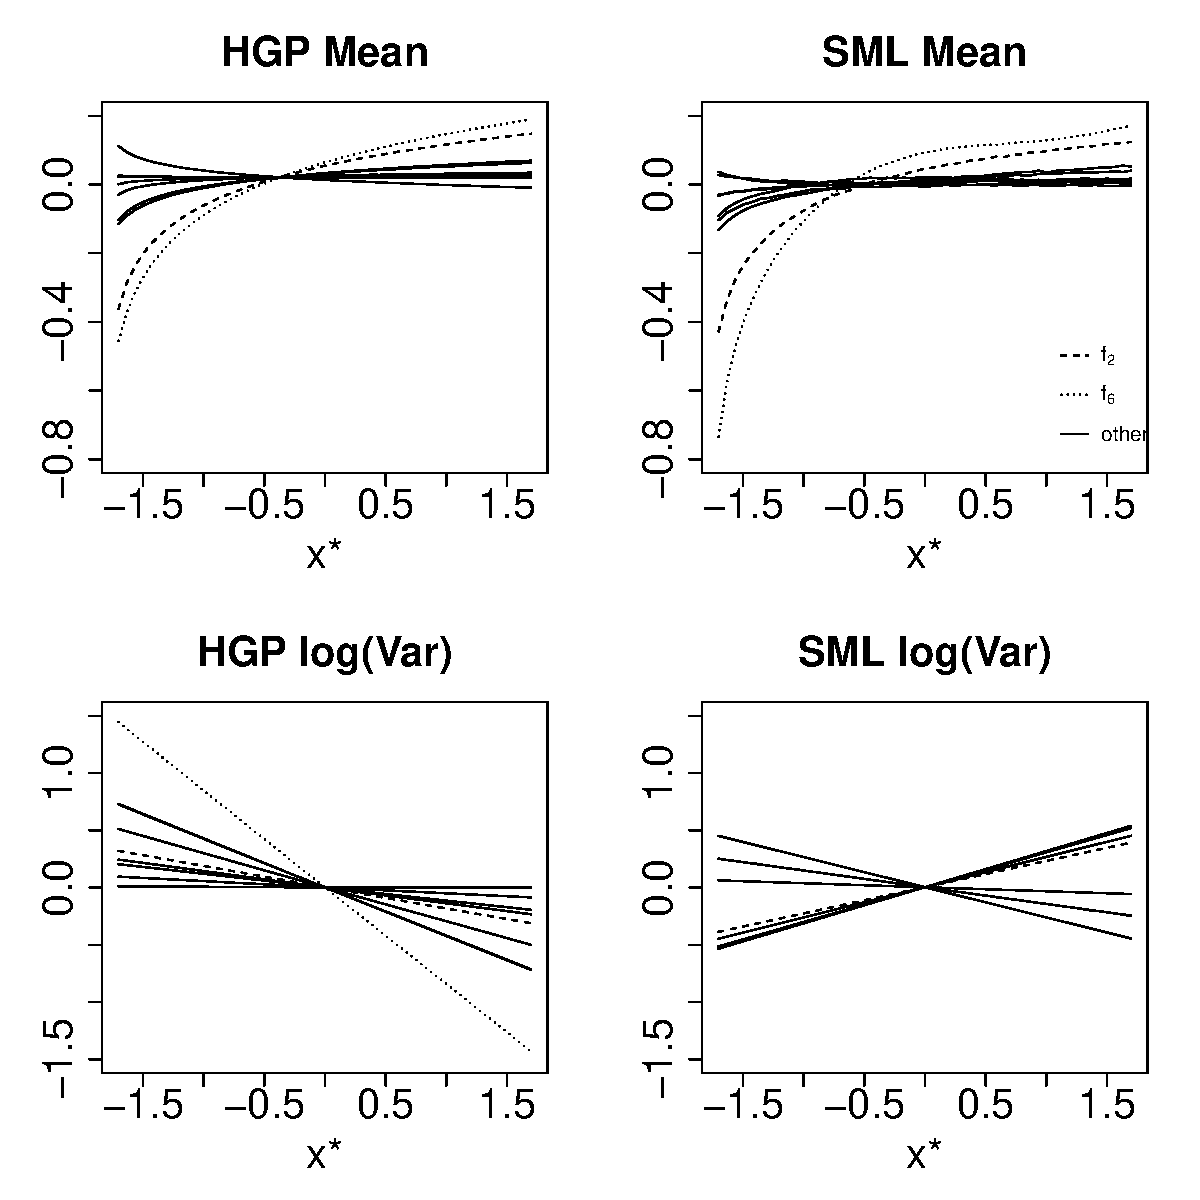
\includegraphics[width=0.9\textwidth]{fig-sensitivity/main-effects-all.pdf}
     \caption{Main effect plots under HetGP (left) and SML (right). Top plots correspond to the mean surface and bottom plots to the log variance surface. The dashed lines correspond to $f_2(x_2)$ and $f_2^{\lambda}(x_2)$, dotted lines to $f_6(x_6)$ and $f_6^{\lambda}(x_6)$. The solid lines represent all other main effects. The $x$ axis is on the standardised scale that the emulators were fitted on. Note that the scale of the $y$ axis on the mean plot differs from that of the variance plot.}
  \label{Fig:main-eff-all}
\end{figure}

We see that qualitatively, the plots of main effects (\Cref{Fig:main-eff-all}) agree with the estimated values of $S_i$ and $S^{\lambda}_i$. That is, an input with high $S_i$ exhibits a large range in the main effect plot. The main effect plots for the mean are quite similar with the exception of $f_6(x_6)$. Under SML $f_6(x_6)$ has a much larger range and the shape of $f_6(x_6)$ is different under the two approaches. The HetGP estimate looks very close to $\log(x_6)$; the chosen mean function. This suggests that SML is borrowing information from the cheap simulator to inform the mean response of the expensive simulator and marries up with the (lack of) structure in the residual plots seen earlier (\Cref{Fig:het-resids}, \Cref{Fig:sml-resids}). The main effects for the log variance are quite different under the two emulators. Under HetGP, $x_6$ is highly influential for the log variance, whereas $x_6$ is much less influential under the SML emulator. A stark difference is that the slopes of many of the $f_{i}^{ \lambda }(x_i)$ are of opposite sign under the two emulators. For example, the slope of $f_2^{ \lambda }(x_2)$ under SML is positive which matches up with empirical estimates given in \Cref{Fig:log-vars}.  We believe this is due to SML resolving a kind of weak identifiability issue; when insufficient data is fed to a HetGP emulator, systematic variation can be interpreted as noise. \cref{Fig:log-vars} shows logged sample estimates $\var \{ y(\bx) \} $. Namely, we have plotted $\log s^2(\bx)$ where
\begin{equation}
  s^2(\bx) =  \frac{1}{N-1} \sum_{i = 1}^N \left\{\probit[A(\bx)]_i - \overline{\probit}[A(\bx)]\right\}^2
\end{equation}
is the (estimated) variance of the probit availability, and availability is defined at the mean point-wise availability over the first $5$ years of the wind farm's life time. The $i$ subscript is used to denote replicates at the same value of $\bx$. The \correction{data plotted in \cref{Fig:log-vars} are based} on a round of simulations independent of training data of any emulators. We only varied $x_2$ to construct this plot. Although we were critical of OAT analyses earlier, we can justify fixing the other inputs here as our sensitivity analysis showed the interaction terms were negligible thus varying inputs one-at-a-time is a reasonable way to sense-check the main effect plots.

\begin{figure}
  \centering
  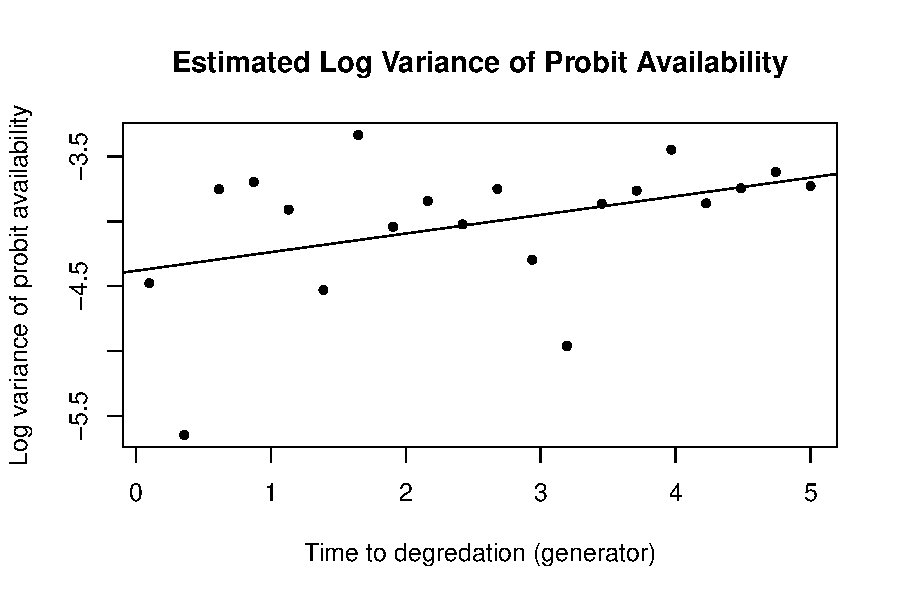
\includegraphics[width = 6in]{sml-het-fig2/log-var-reps2.pdf}
  \caption{Log sample variances of $\probit[A(\bx)]$ at equally spaced points on $[0.1, 5]$. Each estimate is based on $10$ replicates of the expensive version of Athena considered in \cref{Ch:Hetsml} and generated independently of any emulator training data. \label{Fig:log-vars}}
\end{figure}
\section{Conclusions}
We have now performed the necessary analyses to set up a future elicitation procedure. Using the results from either the SML or HetGP emulators the largest contributions to output uncertainty were the failures of the blades ($x_6$) and generator ($x_2$). An equi-tailed $95\%$ credible interval (computed via SML) for $S_2 + S_6$ is $(59,73)\%$ of input uncertainty. Note that this estimate does not include $S_{2,6}$, the contribution of uncertainty due to the interaction between $x_2$ and $x_6$. The simulator appears to be approximately additive, thus $S_{2,6} \approx 0$. The results of the sensitivity analysis were also used to help understand why one of two competing emulators performed worse than the other. A second round of elicitation of $\bx$ would focus mainly on the lifetime parameters of the generator ($x_2$) and the turbine blades ($x_6$), since they jointly contribute to over half of output uncertainty. The other inputs would not be completely neglected since they contribute roughly equal amounts of uncertainty to the log variance. Without an emulator this sensitivity analysis would have taken many months of CPU time. Our SML emulator allowed us to further reduce the amount of time required to construct an adequate emulator by exploiting a computationally cheaper version of the Athena simulator.

One issue that we have not explored here is understanding which input(s) have the largest overall impact on $y(\bx)$. Suppose that, for an $m$ dimensional simulator, the largest $S_i$ is $S_1$ and the smallest is $S_m$. Further suppose that $S^{\lambda}_1$ is the \textit{smallest} sensitivity index for the log variance and $S^{\lambda}_m$ is the \textit{largest}. In such a scenario it is not clear whether $x_1$ is more or less important than $x_m$. In a deterministic setting, if we know the precise value of $\bx$ then we can find $f(\bx)$. In the stochastic case, knowing $\bx$ means we can find the distribution of $y(\bx)$. One way to do this would be to formulate a utility function $U(\bx) = \tilde{U} ( y(\bx))$ and perform an EVPI analysis, on $U(\bx)$. $U(\bx)$ should reflect which aspects of $y(\bx)$ are most critical to our application. For example, if our aim is to find input settings which lead to the average availability, $A(\bx)$, being above some threshold $A^{*}$ then $u(\bx) = \mathbb{I}(A(\bx) > A^{*})$ would be an appropriate utility function (remembering that $\E\{u(\bx)\}  = U(\bx)$). This would be equivalent to emulating, and performing an EVPI analysis on $\Pr (A(\bx) >  A^{*})$.

If the analysis is concerned with understanding which inputs are driving the entire distribution (rather than a single summary), it may be advantageous to borrow ideas from the Bayesian design of experiments literature. In Bayesian design of experiments, one will have a prior specification for the parameters of a statistical model, and the design should aim to maximise a summary of the posterior, such as some notion of difference between prior and posterior \citep{Prangle2022}. A concrete idea would be to construct a HetGP emulator for $y(\cdot)$ then use Kullback-Leibler divergence as a utility function within an EVPI framework. Since, under GP assumptions, $y(\bx)\mid\bx \sim N(\mu(\bx),\lambda^2(\bx))$ we may be able to obtain a tractable analysis by assuming $y(\bx) \sim \mathcal{N}(M, V)$. In particular, if $\bx'$ is a known simulator input, then assuming $y(\bx)$ and $y(\bx')$ are Normally distributed we have
\begin{equation}
  U(\bx') = \text{KL}(y(\bx') || y(\bx)) = \log \left( \frac{\hat{\lambda}(\bx')}{\sqrt{V}} \right) + \frac{\hat{\lambda}^2(\bx') + (m^{*}(\bx') - M)^2}{2V} - \frac{1}{2}.
\end{equation}
Then, by an EVPI analysis, the input $i$ with largest EVPI would be the most influential input on the distribution of $y(\cdot)$. Since, with an emulator, $m^{*}$ and $\lambda^2(\bx)$ are quick to compute, this analysis should be tractable within a frequentist framework or an Empirical Bayes framework like the emulators described in \cref{Ch:Hetsml}. A fully Bayesian equivalent to the analysis would have to average over $\pi \{ y(\cdot) \mid \mathcal{D} \}$. This is similar to the approach taken by \citet{Oakley2009}, who performs an EVPI analysis, assisted by emulators, to deduce which of three medical treatments offers the most viable solution. EVPI analysis comes into play as a way to check the robustness of the optimal decision. This is perhaps more useful than performing PSA on the mean and log variance separately. Of course, performing PSA on the mean and variance has many valid use cases. It allows us to investigate the behaviour of a complex, black-box stochastic simulator. We used the results of PSA to diagnose potential issues with an emulator We used the fact that the main effect plots of the log variance generated by HetGP were inconsistent with our knowledge of Athena to understand that the HetGP emulator was confusing systematic and random variation. In other words, we extended this idea to \textit{emulator} validation. On a similar vein, \citet{Kennedy2006} used the main effect plots to verify that a vegetation model produced sensible outputs. The outputs were deemed unusual which led to the discovery of a bug in the simulator under study.
\end{chapter}

  
% --------------------------------------------------------------
\begin{chapter}{Decision Making with Complex Models \label{Chap:optimisation}}

In many settings, a model --- of any complexity --- can be constructed and then deployed to aid decision making. Bayesian decision theory gives us a mature and coherent framework for combining the decision maker's prior beliefs and preferences with a model, including complex stochastic simulators. Recall that if the decision maker represents their preferences for a decision $\bx \in \mathcal{X}$ by a utility function $u(\bx, \btheta)$, they represent their beliefs about all uncertain quantities by a prior distribution $\btheta \sim \pi(\btheta)$ and the expected utility of a decision is $U(\bx) = \E_{\btheta} \{ u(\bx, \btheta) \}$, then the optimal decision is defined as
\begin{equation}
 \bx^{*} = \argmax_{\bx \in \mathcal{X}} U(\bx).
\end{equation}
Prior beliefs, $\pi(\btheta)$, should be replaced by posterior beliefs, $\pi(\btheta | \by)$, when relevant data, $\by$, are available.

Once the decision problem has been defined by an appropriate belief structure as above, the decision problem is reduced to an optimisation problem. Although the problem is `reduced', the enormous literature on mathematical and numerical optimisation should serve as a warning that the reduced problem is usually far from trivial. The difficulty is amplified when the utility function is expensive to compute, is noisy and no gradient information is available. This can be because $U(\bx)$ itself is expensive to compute or depends on the output of one or more computationally expensive simulators \citep{Williamson2012}. Both situations are commonly seen in Bayesian design of experiments or subjective Bayesian analyses when viewing a large collection of samples from the posterior distribution with negligible autocorrelation as the output of a computationally expensive simulation (e.g. a long run of an MCMC scheme) \citep{Ryan2016, Vernon2022bayes}. Our analysis will use relatively simple utility functions; however, the utility function itself depends on output of the Athena model. Therefore, $U(\bx)$ will be expensive to compute.

We now discuss the various types of optimisation problem that arise and methods to solve them.

\section{Discrete problems}
\subsection{Small, discrete problems}
Suppose that there is no obvious structure to the decision problem, or the number of decisions that can be taken is small. In a wind farm setting this could be considering where to place the farm from a small number of candidate locations. If we consider $n$ locations $\mathcal{X} = \{ \bx_1, \bx_2, \ldots \bx_n \}$ then the best we can do is just evaluate $U(\bx_i)$ for each $i$.

When the decision is made under uncertainty, the simplest approach is to use a Monte Carlo approximation of $U(\bx_i)$. If evaluating $u(\bx, \btheta)$ is expensive because, for example, the utility of a decision depends on the result of a complex computer model, we may wish to construct an emulator for $u(\cdot)$ as a function of uncertain quantities $\bm{\btheta}$ and decision variables $\bx$. That is, construct a surrogate, $\hat{u}(\bx, \btheta)$ and propagate beliefs $\pi(\bm{\btheta})$ through $\hat{u}(\bx, \btheta)$. This is precisely what \citet{Oakley2009} does, and achieves a tractable approximation to $U(\bx_i)$ via a GP emulator.

Another option for discrete problems is Thompson Sampling (TS). If the number of simulator evaluations we can make is limited, we may want to carefully allocate simulator runs in a sequential manner. TS originated in two-armed bandit problems \citep{Thompson1933} and has enjoyed recent success in multi-armed bandit problems since it is simple but effective \citep{Scott2010, Chapelle2011}. The approach to solving a multi-armed bandit problem via TS is to randomly allocate simulator runs one-by-one to a pre-defined set of inputs. This sequential allocation balances exploitation of inputs which are likely to give rise to good solutions whilst acknowledging that simulator outputs are uncertain, thus the uncertainty should be resolved via exploring the decision space.

When the decision set is small and discrete we may be able to phrase the problem as a multi-armed bandit problem. For example, suppose we have $U(\bx) = \p (A(\bx) > A^{*}) = \E \{\mathbb{I}(A(\bx) > A^{*}) \} $, and we have a small number of distinct values of $\bx$ corresponding to discrete decisions. These decisions, for example, could be a small collection of different locations at which the wind farm could be constructed. Running the Athena simulator at a candidate decision $\bx$ will give us an availability which is either above $A^{*}$ or not. After $n$ simulator runs at different values of $\bx$ (with some replication) we are able to obtain probabalistic estimates for each $U(\bx)$. Since, in this example, $U(\bx)$ is a probability, a Beta distribution would be an appropriate probabalistic representation of $U(\bx)$. The Beta prior distribution allows us to estimate $U(\bx) = P(A(\bx) > A^{*})$ via conjugate Bayesian inference. If, prior to running any simulations, $U(\bx_i) \sim Beta(a_{i,0}, b_{i,0})$, then once we have evaluated $u(\cdot)$ $n_i > 0$ times at simulator input $\bx_i$, the posterior distribution will be $Beta(a_{i,n_i}, b_{i, n_i})$ where
\begin{align}
 a_{i, n_i} & = a_{i, 0} + \sum_{j = 1}^{n_i} \mathbb{I} \left\{ A(\bx_i)_j > A^{*} \right\} \nonumber\\
 b_{i, n_i} & = b_{i, 0} + \sum_{j = 1}^{n_i} \mathbb{I} \left\{ A(\bx_i)_j \leq A^{*} \right\}\nonumber
\end{align}
where $A(\bx_i)_j$ is the $j$th draw of $A(\bx_i)$. If $n_i = 0$ then the prior cannot be updated; our prior beliefs will be the representation of our knowledge. TS tells us to next run the simulator at the input which maximises
\begin{equation}
 \bx_j = \argmax_{i \in \{1, 2, \ldots, n \} } \tilde{U}(\bx_i)
\end{equation}
where $\tilde{U}(\bx_i)$ are independent, random draws of $U(\bx_i) \sim Beta(a_{i, n_i}, b_{i, n_i})$. The random draws induce an exploration-exploitation trade-off. Randomness allows for exploration as it accounts for uncertainty about the $U(\bx_i)$. Exploitation comes into play though the posterior distributions. If the posterior density of $U(\bx_i)$ is concentrated about large values of $U(\bx_i)$, then the probability that the simulator is run at $\bx_i$ will increase. We can also allow for exploitation of prior knowledge via the prior; $a_{i,0} \in \N$ and $b_{i,0} \in \N$ can be interpreted as \textit{a priori} counts for the events $A(\bx_i) > A^{*}$ and $A(\bx_i) \leq A^{*}$ respectively. This approach can be extended to continuous problems, which is considered later.
\subsection{Structured, discrete problems}
Some decision problems are discrete in nature but far too complex for a brute force computation. The lack of smoothness in such problems makes emulation difficult. In some situations we cannot solve the decision problem exactly because of these computational constraints. We must settle for the best solution possible in the time available.

In complex, discrete problems the expected utility surface can be very rough with respect to the decision space. A well-known example of such a problem is the Travelling Salesman Problem (TSP) in which a salesman aims to visit a fixed set of locations, by traversing the edges of a graph, in such a way that costs are minimised. Phrasing as a decision problem, if $\ell(\bx)$ is the cost of the path taken by the salesman, we would take $U(\bx) \propto \ell(\bx)$. In this case, a small change in the path might lead to a not so small change in $U(\bx)$, that is, if $||\bx - \bx'||$ is small, there is no reason to believe that $||U(\bx) - U(\bx')||$ is also small \citep{Gutin2007}.

A mathematically simple approach is a random search. Take a random sample $\mathcal{X}_0 = \{ \bx_1, \bx_2, \ldots, \bx_n\}$ from $\mathcal{X}$. Then an approximation to the optimal decision is $\hat{\bx} = \argmax_{\bx \in X_0} U(\bx)$. If the computational budget is large enough, we would find $\bx^{*}$. In practice, this can be a big ``if''. Convergence to the optimum requires many evaluations of $U(\bx)$ when knowledge of $U(\bx)$ is ignored \citep{Kan1989}. Beyond this, random search serves as a benchmark: if random search does better than a seemingly more intelligent method, then perhaps the method is not as intelligent as first thought.

An adaptation of (purely) random search is stochastic optimisation. A common example is simulated annealing (SA), which is inspired by the process of annealing in metallurgy \citep{Kirkpatrick1983, Schneider2006}. SA is one of many stochastic optimisers, and can perform well when the decision surface is very rough. Given a candidate solution $\bx'$ and a `current' solution $\bx_t$ we take $\bx_{t+1} = X_{t+1}$ where $X_{t+1}$ is a random variable which takes the value $\bx'$ with probability $\alpha( \bx' \mid \bx_{t}, t)$ and $\bx_t$ otherwise. The candidate decision will typically be a modified version of $\bx_t$. If the decision space is a subset of $\R^k$, we might form $\bx'$ by setting $\bx' = \bx_t + \mathcal{N}(0, \sigma^2I_k)$ where $\sigma^2$ is a tuning parameter. For discrete problems, we may randomly change individual aspects of $\bx$ to construct $\bx'$. For example, if $\bx$ is a vector of binary values, we may set $x_i' = 1 - x_i$ for some randomly chosen $i$. Typically $\alpha(\bx' \mid \bx_{t}, t)$ should favour $\bx'$ for small values of $t$, corresponding to exploratory behaviour in early stages, but as $t$ increases, $\alpha(\bx' \mid \bx_{t}, t)$ should begin to favour $\argmax \{U(\bx_t), U(\bx')\}$, corresponding to increasing levels of exploitation. A common form for alpha is
\begin{equation}
 \alpha(\bx' \mid \bx_{t}, t) = \min \left\{ \exp\left[-\frac{U(\bx_t) - U(\bx')}{Kt}\right], 1\right\}
\end{equation}
where $K$ is a tuning parameter which controls the rate of the annealing schedule. SA can be thought of as a random walk which is designed to maximise $U(\bx)$. SA cannot not really exploit any structure in $U(\bx)$ (and is designed for situations where $U(\bx)$ has little structure) thus may require many evaluations of $U(\bx)$ to find a close-to-optimal solution. Within the emulation literature, SA has been successful in providing optimal Latin hypercube designs \citep{Morris1995, Pholdee2015}.

A discrete structure which can be exploited through surrogate modelling is permutations. Consider a set of tasks $\{T_1, T_2, \ldots, T_J\}$. If there are $J$ tasks to complete, then $J!$ permutations need to be considered. For moderately small $J$, $J!$ can be very large and grows incredibly quickly ($3! = 6$, $6! = 720$, $10! = 3628800$). Computing $U(\bx)$ for all possible $\bx$ can quickly become very time consuming, especially if $U(\cdot)$ is expensive. To alleviate this, \citet{Wilson2018} use a surrogate inspired by the Benter model \citep{Benter1994} to efficiently find an approximate solution to their permutation-based problem.
\subsection{Continuous problems}
If the decision space is continuous, e.g. $\bx \in \mathcal{X} \subseteq \mathbb{R}^n$ and we have relatively easy access to $U(\bx)$, we can use standard optimisation routines like \verb|optim| in \verb|R|. Continuity allows us to embrace calculus when we have easy access to $U(\bx)$. By `easy access' we mean that $U(\bx)$ is available in closed form, or we have access to highly accurate approximations such as Monte Carlo estimates with negligible standard errors.

However, evaluation of $U$ might be sufficiently difficult to make standard optimisation methods cumbersome. When evaluations of $U(\bx)$ are limited for computational or financial reasons, such as running simulations in a pay-per-usage cloud server, requires collection of primary data, human interaction or is otherwise computationally expensive, we may use a surrogate to reduce optimisation costs \citep{Tresidder2012, Astudillo2020}.

Broadly, we can use a surrogate to perform optimisation in two ways. The first way is to construct a one-shot design (via, for example, a Latin Hypercube) to construct an emulator or surrogate $\hat{U}(\bx)$. Maximising $\hat{U}(\bx)$ will provide an approximate solution to the decision problem. For examples of this approach see \citep{Wilson2018, Overstall2017}. The second way is to view optimisation as a sequential design problem, which we explore in the next section.

\section{Bayesian optimisation}
Instead of directly maximising the surrogate, $\hat{U}(\bx)$, it may be advantageous to use our knowledge of $U(\bx)$, expressed as a posterior distribution, to guide us towards values of $\bx$ which are likely to improve on the largest value of $U(\bx)$ seen so far. This is essentially what numerical optimisation does. A standard Newton-Raphson scheme uses the gradient of $U(\bx)$ to speculate where a larger value of $U(\bx)$ may lie. Newton-Raphson uses only local knowledge of $U(\bx)$. Gaussian processes have a global \emph{and} a local understanding of $U(\cdot)$, this can be leveraged.

An approach known as \textit{Bayesian Optimisation} (BayesOpt) uses global and local knowledge, expressed via a posterior distribution, to maximise $U(\bx)$. The core idea behind BayesOpt is to construct an emulator for $U(\bx)$ and use this to guide our search towards $\bx^{*}$ \citep{Frazier2018}. Although much of the BayesOpt language is plagued by machine learning jargon, BayesOpt is actually a form of sequential design. BayesOpt has been found to be useful in a variety of optimisation problems where $U(\bx)$ has some, or even all, of the following properties
\begin{itemize}
 \item $U(\bx)$ is costly to evaluate
 \item $U(\bx)$ possess multiple local optima
 \item derivatives, $\frac{\partial U(\bx)}{\partial x_i}$, are not available
 \item $U(\bx)$ is thought to be quite smooth
 \item $\bx$ is of not too large dimension (less than about $20$).
\end{itemize}
The Athena simulator possesses many of these properties. In particular, we know that it is expensive to evaluate, has no closed form gradient expressions and we think that many quantities output by Athena are reasonably smooth. We do not know how many local optima Athena has, and that may depend on which input-output combinations are used for optimisation.

BayesOpt is a promising framework for solving decision problems with the Athena simulator. Not all of these properties have to hold for BayesOpt to be a suitable approach. For example, knowledge about maxima or gradient information can be leveraged \citep{Wu2017, Nguyen2020}. The key properties are that $U(\bx)$ is costly and smooth; if it were not, other methods could be more appropriate. A common application of BayesOpt is tuning machine learning models \citep{Joy2016, Snoek2012}. BayesOpt dates back to at least \citet{Mockus1975} who used (Bayesian) linear models as the surrogate. The modern incarnation of BayesOpt has stemmed from \citet{Jones1998} who popularised the use of more flexible covariance structures (for example, the squared exponential) within BayesOpt. BayesOpt can be viewed as a sequential design strategy for global maximisation (or minimisation) of expensive black-box functions, see \citet{Frazier2018} for an overview.

We will take a diversion from the Athena simulator and decision making to consider BayesOpt for arbitrary functions, rather than utility functions. Suppose we observe $y(\bx) = f(\bx) + \varepsilon(\bx)$ where $f(\cdot)$ is the function to be maximised and $\varepsilon(\bx)$ is (possibly input dependent) noise, which is assumed to be independent of other error terms, Gaussian and additive. We start by specifying the joint model for $(\by^T, f(\bx))$ and use the conditional Normal equations to provide the posterior moments for $f(\bx) \mid \by$
\begin{align}
 \begin{pmatrix} \by \\ f(\bx) \end{pmatrix}
  &\sim \mathcal{N} \left\{
  \begin{pmatrix} \mu(X) \\ \mu(\bx) \end{pmatrix}, \begin{pmatrix} \Sigma_{X, X} & \Sigma_{X, \bx} \\ \Sigma_{\bx, X} & \sigma^2 \end{pmatrix}
  \right\} \\
  f(\bx) \mid \by &\sim \mathcal{N}(m^{*}(\bx), v^{*}(\bx) )
\end{align}
where $X$ are the locations at which the simulator has been run, $\mu(\cdot)$ is the prior mean function, $\Sigma_{X, X} = \var\{\by\}$, $\sigma^2 = \var\{f(\bx)\}$, $\Sigma_{X, \bx} = \Sigma_{\bx, X}^T = \cov\{y(X), f(\bx)\}$ and $m^{*}(\bx)$ and $v^{*}(\bx)$ are the posterior mean and variance, as found by the multivariate Normal equations; \cref{Eq:MV1} and \cref{Eq:MV2}.
\subsection{Acquisition functions}
Once an emulator has been fit to a small collection of initialisation runs, we can start to use the emulator to make intelligent choices about where to next run the simulator so that $f(\bx)$ can be efficiently optimised. The device that allows us to make decisions about where to next evaluate $f(\bx)$ is an \textit{acquisition function}. The acquisition function is a function of $\bx$ and the posterior distribution on $f(\bx)$ which aims to find large values of $f(\bx)$. We introduce new notation for the posterior on $f(\cdot)$ which is better suited to online learning/sequential inference. Suppose we have observed $n$ runs of the simulator: $\mathcal{D}_n = \{(\bx_1, y_1), (\bx_2, y_2), \ldots, (\bx_n, y_n)\}$. The `time $n$' posterior for $f(\cdot)$ (after observing $n$ runs) is denoted $\pi_n(f(\cdot) \mid \mathcal{D}_n, \Theta_n)$ where $\Theta_n$ are the time $n$ GP hyperparameters. We will abuse notation here and use $\pi_n(f(\cdot))$ as shorthand for $\pi_n(f(\cdot) \mid \mathcal{D}_n, \Theta_n)$. We then define, using the dummy variable $y = f(\bx)$,
\begin{equation}
 \E_n\{g(f(\bx))\} = \int_{-\infty}^{\infty} g(v) \pi_n(y) \,\dd v
\end{equation}
as the expected value of $g(f(\bx))$ with respect to $\pi_n(f(\bx))$, for any function $g(\cdot)$ at a known input $\bx$. This additional notation is useful since acquisition functions can often be expressed as expectations of a function of $f(\bx)$, having observed $n$ simulator runs. This means that many acquisition functions have a decision theoretic justification because they are expressed as expectations of utility functions. Having observed $n$ simulator runs, and \correction{assuming that $\E_n(f(\bx))$ has a single global optimum,} the time $n$ optimal solution is
\begin{equation}
 \hat{\bx}_n = \argmax_{\bx \in X_n} \E_n \{ f(\bx) \} \label{Eq:best-so-far}
\end{equation}
where $X_n$ is the set of input configurations at which the simulator has been run. When $f(\cdot)$ is a deterministic function, $\hat{\bx}$ corresponds to the input which, so far, has given the largest function output. This is precisely the value that would be used under any other optimiser. When $f(\cdot)$ is observed with noise, \cref{Eq:best-so-far} is the value of $\bx$ leading to the largest posterior mean. This follows naturally from Bayesian decision theory. We now introduce some more notation to allow a fluent discussion of common acquisition functions. Let $y^{*}_n = \E_n \{ f(\hat{\bx}_n) \}$, let $\mu_n(\bx) = \E_n \{ f(\bx) \}$ and let $\sigma^2_n(\bx) = \var_n\{ f(\bx) \} = \E_n \left\{ \left[ f(\bx) - \mu_n(\bx) \right]^2 \right\}$, where $\bx \in \mathcal{X}$ is any valid input.
\subsubsection{Probability of improvement}
The first acquisition function we encounter is the probability of improvement (PI) denoted $\alpha_{PI}$. Consider the following utility function over possible values of $f(\bx)$:
\begin{equation}
 \tilde{\alpha}_{PI}(\bx) =
 \begin{cases}
  1,& f(\bx) > y^{*}_n \\
  0,& f(\bx) \leq y^{*}_n
 \end{cases}
\end{equation}
that is, an indicator utility function returning $1$ when we improve upon $y_n^{*}$ and returning $0$ when there is no improvement. This expresses the belief that all improvements, regardless of size, are equally preferable. We then have $\alpha_{PI}(\bx) = \E_n \{ \tilde{\alpha}_{PI}(\bx) \}$. The expectation of an indicator function is the probability of the event in question, thus we have
\begin{align}
 \alpha_{PI}(\bx) &= \p(f(\bx) > y^{*}_n)\label{Eq:prob-imp}\\
  &= \Phi\left(\frac{ \mu_{n}(\bx) - y^{*}_n }{\sigma_{n}(\bx)}\right). \label{Eq:prob-imp-gp}
\end{align}
Regardless of the chosen statistical model, \Cref{Eq:prob-imp} provides the probability of improvement; this will be available in closed form for a large class of statistical models. If the closed form is not available, a highly accurate approximation is likely to be built into popular scientific computing libraries. Under GP assumptions, the probability of improvement can be expressed as \Cref{Eq:prob-imp-gp} which, technically, is not tractable but good approximations are widely available, for example, \texttt{pnorm()} from \texttt{R}.
\subsubsection{Expected improvement}
A criticism of PI as an acquisition function is that PI sees all possible improvements as equally good, regardless of the magnitude of the improvement. Suppose that $y^{*}_n = 0$ and further suppose $f(\bx_1) \sim N(0, 1)$ and $f(\bx_2) \sim N(0, 10)$. We see that $\alpha_{PI}(\bx_1) = \alpha_{PI}(\bx_2) = 0.5$, therefore, this BayesOpt scheme views $\bx_1$ and $\bx_2$ as equally promising. However, the potential gains under $\bx_2$ are much larger than the potential gains under $\bx_1$. The nature of PI can be investigated via partial derivatives. We see that $\frac{\partial \alpha_{PI}(\bx)}{\partial \mu_n(\bx)} = \frac{1}{\sigma_n(\bx)}\phi\left( \frac{\mu_n(\bx) - y^{*}_n}{\sigma_n(\bx)} \right) > 0$ thus, increasing $\mu_n(\bx)$ increases $\alpha_{PI}(\bx)$. Therefore, inputs corresponding to function values with large predictive means are favoured. However, $\frac{\partial \alpha_{PI}(\bx)}{\partial \sigma_n(\bx)} = -\frac{\mu_n(\bx) - y^{*}_n}{\sigma_n(\bx)^2}\phi\left( \frac{\mu_n(\bx) - y^{*}_n}{\sigma_n(\bx)} \right)$. The sign of this expression depends on $\mu_n(\bx) - y^{*}_n$. In particular, $\text{sign}\, \left\{\frac{\partial \alpha_{PI}(\bx)}{\partial \sigma_n(\bx)}\right\} = \text{sign}\,\{y^{*}_n - \mu_n(\bx)\}$, therefore increasing $\sigma_n(\bx)$ increases $\alpha_{PI}(\bx)$ whenever $\mu_n(\bx) < y^{*}_n$ but decreases $\alpha_{PI}(\bx)$ when $\mu_n(\bx) > y^{*}(\bx)$ and $\alpha_{PI}(\bx) = 0.5$ when $\mu_n(\bx) = y^{*}(\bx)$. This means that we tend not to explore areas in which $f(\bx)$ is uncertain but has moderately large values of $\mu_n(\bx)$. The way PI deals with uncertainty is unsatisfactory; if $f(\bx)$ is thought to be large but $\var\{f(\bx)\}$ is also large, this is a region of the input space that should be explored further as the potential gains are large. This criticism can be boiled down to the fact that PI does not consider how large the potential change in $y_n^{*}$ is.

This motivates \textit{Expected Improvement} (EI) which gives a reward proportional to the improvement. First we define the improvement by
\begin{equation}
 \tilde{\alpha}_{EI}(\bx) = \max\{0, f(\bx)-y^{*}_n\}.
\end{equation}
This is intuitive: if $f(\bx) \leq y^{*}_n$ our best value has not improved. But if $f(\bx) > y^{*}_n$ then we have improved our current best value of $f(\cdot)$ by $f(\bx) - y^{*}_n$. Now since $f(\bx)$ is unknown, we integrate out $f(\bx)$, which has density $\pi_n(f(\bx))$, and thus the EI is
\begin{equation}
 \alpha_{EI}(\bx) = \E_n \{ \tilde{\alpha}_{EI}(\bx) \}.
\end{equation}
Under standard GP assumptions, we have an analytic expression for EI in terms of the Normal CDF and PDF. We aim to maximise $f(\cdot)$, so the acquisition function can be expressed as \citep{Pourmohamad2021}:
\begin{equation}
 \alpha_{EI}(\bx) = \begin{cases}
           \sigma_n(\bx)\phi\left(\frac{\mu_n(\bx)-y^{*}_n}{\sigma_n(\bx)}\right) + (\mu_n(\bx) - y_n^{*})\Phi\left(\frac{\mu_n(\bx)-y^{*}_n}{\sigma_n(\bx)}\right),&  \sigma_n(\bx) > 0 \\
           0, &  \sigma_n(\bx) = 0
           \end{cases}. \label{Eq:EI-defn}
\end{equation}
The EI is $0$ when $\sigma_n(\bx) = 0$ because $\sigma_n(\bx) = 0$ if, and only if, we know the value of $f(\bx)$ precisely. $f(\bx)$ will either be $y_n^{*}$ or be smaller than $y_n^{*}$ and hence offers no improvement. Although EI was constructed with deterministic problems in mind, it generalises naturally to the stochastic case. The exploitation-exploration trade-off under EI is fairly transparent. The first term of EI is multiplied by $\sigma_n(\bx)$, thus large uncertainty leads to larger values of $\alpha_{EI}$. The second term is multiplied by $\mu_n(\bx) - y_n^{*}$, thus large mean predictions typically increase EI. Applying basic calculus rules to \cref{Eq:EI-defn} leads to $\frac{\partial \alpha_{EI}(\bx)}{\partial \mu_n(\bx)} = \Phi \left( \frac{\mu_n(\bx) - y^{*}_n}{\sigma_n(\bx)} \right) > 0$ and $\frac{\partial \alpha_{EI}(\bx)}{\partial \sigma_n(\bx)} = \phi \left( \frac{\mu_n(\bx) - y^{*}_n}{\sigma_n(\bx)} \right) > 0$, thus EI increases with both $\mu_n(\bx)$ and $\sigma_n(\bx)$. That is, for fixed $\mu_n(\bx)$, a more uncertain value is a preferred input to run the simulator at, whilst if $\sigma_n(\bx)$ is fixed we will run the simulator at the input with greatest predicted value.

There are many extensions to EI which take into account problem structure. Examples include optimisation under unknown (black-box) constraints which learns the optimum input/output and the constraints \citep{Gramacy2010}. Batch (or ``multi-point'') EI runs the simulator at multiple, promising solutions simultaneously to take advantage of abundant cores in a parallel computing setting \citep{Marmin2015, Diessner2022}.
\subsubsection{Upper credible bound}
Another common acquisition function is the upper credible bound, or upper confidence bound, depending on the chosen interpretation of probability \citep{Srinivas2009}. Both can be abbreviated to UCB.
The UCB acquisition function is, under a GP model for $f(\cdot)$,
\begin{equation}
 \alpha_{UCB}(\bx \mid \nu_n) = \mu_n(\bx) + \nu_n \sigma_n(\bx). \label{Eq:ucb}
\end{equation}
where $\nu_n > 0$ are a sequence of tuning parameters controlling the exploration-exploitation trade-off. UCB was proposed with maximisation in mind but if minimisation is required we can use the lower credible/confidence bound instead.
\begin{equation}
 \alpha_{LCB}(\bx \mid \nu_n) = \mu_n(\bx) - \nu_n \sigma_n(\bx).
\end{equation}
For many statistical models, \cref{Eq:ucb} is an upper credible/confidence bound. We can adjust $\nu_n$ as appropriate. This means that in principle, UCB gives a tractable acquisition function for $f(\bx)$, whenever the chosen emulator has a tractable mean and variance. If $f(\bx)$ is not modelled \textit{a priori} by a GP, the expected improvement would likely be intractable.
 If desired, we can take $\nu_n = \nu$ for all $n$. Now since UCB is a linear combination of the posterior mean and standard deviation, the exploration-exploitation trade-off is transparent. Increasing $\mu_n(\bx)$ or $\sigma_n(\bx)$ whilst the other remains fixed clearly increases $\alpha_{UCB}(\bx \mid \nu_n)$. The trade off is controlled by $\nu_n$. Setting $\nu_n = 0$ leads to a pure exploitation regime: maximise the posterior mean. Letting $\nu_n \to \infty$ leads to picking the point with highest uncertainty, which is essentially ALM (\cref{Eq:std-alm}). Choosing a moderate value of $\nu_n$ leads to an exploration-exploitation compromise. The UCB acquisition function is sometimes called an `optimistic' approach; we are choosing $\bx_{n+1}$ based on an upper estimate for $f(\bx_{n+1})$.

Although not immediately obvious, we can actually write $\alpha_{UCB}(\bx)$ as the expected value of a random variable. \citet{JamesWilson2018} show that
\begin{equation}
 \alpha_{UCB}(\bx \mid \nu_n) = \int_{-\infty}^{\infty}\frac{\left( \mu_n(\bx) + |f(\bx) - \mu_n(\bx)| \right)}{\sqrt{2 \pi \tilde{\sigma}^2}} \exp \left\{ -\frac{(f(\bx) - \mu_n(\bx))^2}{2 \tilde{\sigma}^2} \right\} \dd f(\bx)
\end{equation}
where $\tilde{\sigma} = \sqrt{2 \pi \nu_n} \sigma$. This means that the UCB acquisition can be written as the following expectation
\begin{equation}
  \alpha_{UCB}(\bx \mid \nu_n) =\E_{\tilde{y}} \{\tilde{y}\}
\end{equation}
where $\tilde{y} \sim tr\mathcal{N}(\mu(\bx), \tilde{\sigma}^2(\bx); \mu(\bx), \infty)$ where $tr\mathcal{N}(m, s^2; a, b)$ denotes a Normal distribution truncated below at $a$, above at $b$ and the distribution to be truncated is $\mathcal{N}(m ,s^2)$. Therefore $\alpha_{UCB}(\bx)$ can be interpreted, in a decision theoretic context, as the expected value of a linearly transformed and truncated version of $f(\bx)$. This is quite difficult to interpret but this representation of UCB was constructed with computation, not interpretation, in mind \citep{Wilson2017}.
\subsubsection{Thompson sampling}
There is a stochastic approach to BayesOpt; Thompson sampling (TS). By stochastic, we mean that the acquisition function is randomly generated. Whether the simulator is stochastic or deterministic is not critical in this context. The idea behind TS is to draw a random function $g(\cdot) \sim \pi_n(f(\cdot))$ and then use $g(\cdot)$ as an acquisition function. The next point at which to run $f(\bx)$ is then given by the maximiser of this drawn function:
\begin{equation}
 \bx_{n+1} = \argmax_{\bx \in \calX} g(\bx).
\end{equation}
We discussed earlier that TS is useful in multi-armed bandit problems. With a GP framework, for problems defined over a continuous domain, a full draw from $\pi_n(f(\cdot))$ is impossible; this in an object of infinite dimension. The best we can do is draw $g(\tilde{X})$ from $\pi_n(f(\tilde{X}))$ where $\tilde{X}$ is a large, but finite, collection of inputs. This can cause problems in high dimensional settings due to the curse of dimensionality; $\tilde{X}$ will almost always be sparse within the input space. This can be combated by `extending' the realised function by adding rows to the lower Cholesky decomposition of $\var_n \{ f(\tilde{X}) \}$. Algorithms for extending the Cholesky decomposition are discussed by \citet{Higham2009}. This means that maximising $g(\cdot)$ when the decision space is either continuous or large and discrete is difficult. However, the three earlier acquisition functions all need to be maximised via some inner optimisation routine like \verb|optim|. The TS acquisition is trivially maximised via a lookup table.

The discussed acquisition functions are plotted in \Cref{Fig:acq-fns}. They all correspond to the function
\begin{equation}
f(x) = 0.6 \sin (2 \pi x) + 2 \cos (3 \pi x) + \sin (4 \pi x) + 2x \label{Eq:example-function}
\end{equation}
and corresponding emulator in \Cref{Fig:example-fn}. In this particular example, PI, EI and UCB are all maximised in roughly the same place (in the region of $0.6$--$0.8$), which happens to be close to the true maximiser. One TS acquisition function (red) is maximised quite far away from the true maximiser ($\hat{x} \approx 0.5$). This is because the emulator is exhibiting large uncertainty across much of the input space. The other two TS acquisition functions (black and green) and maximised close to the true maximiser. Remember that the acquisition functions are suggesting suitable locations to run the simulator rather than a prediction of where the maximum is.
\begin{figure}[h]
 \centering
 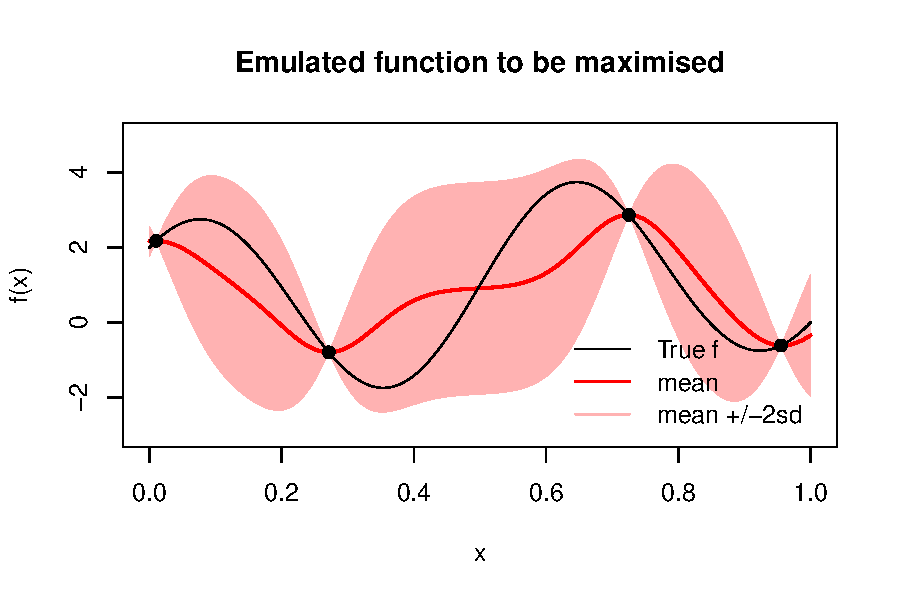
\includegraphics[width=\textwidth]{fig-optim/example-fn-to-maximise.pdf}
 \caption{A function, f(x), given by \cref{Eq:example-function}, to be optimised via BayesOpt with a corresponding emulator. The unknown function to be optimised is deterministic and given by the black line. The emulator mean is given by the solid red line and the translucent red region represents a $95\%$ probability band for $f(x)$. Plots of acquisition functions corresponding to this emulator are in \cref{Fig:acq-fns}.  \label{Fig:example-fn}}
\end{figure}
\begin{figure}[h]
 \centering
 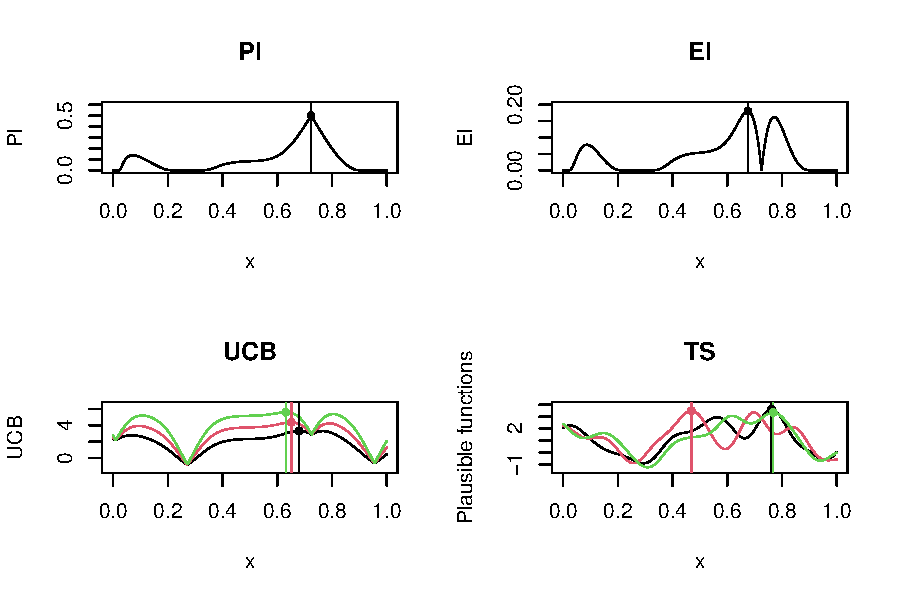
\includegraphics[width=0.8\textwidth]{fig-optim/example-acquisitions.pdf}
 \caption{Plots of acquisition functions for the function and emulator in \Cref{Fig:example-fn}. Vertical lines correspond to the maximiser of the acquisition function with the bullet being the the coordinates of the maximum. Three possible acquisition functions for UCB are shown corresponding to $\nu = 1, 2, 3$ and three random draws of $f(\cdot)$ are shown for TS. \label{Fig:acq-fns}}
\end{figure}
\subsection{Online GP updates for efficient BayesOpt}
BayesOpt is a sequential design problem. The emulator is updated as simulator runs arrive. GP prediction depends on the inversion of an $n \times n$ matrix. Matrix inversion is well known to be a slow (usually $\mathcal{O}(n^3)$) and numerically unstable operation.

By constructing a partition of $\Sigma_{n+1}$, the time $n+1$ precision matrix $\Omega_{n+1}$ can be expressed in terms of $\Omega_n = \Sigma_n^{-1}$ and the partitioned $\Sigma_{n+1}$. This partitioned representation is numerically stable and fast to compute. Consider the following partition of $\Sigma_{n+1}$
 \begin{equation}
 \Sigma_{n+1} = \begin{pmatrix}
         \Sigma_n + \lambda^2(X_n)I_n & c(\bx_{n+1}, X_n) \\
         c(\bx_{n+1}, X_n)^T & \sigma^2(\bx_{n+1}))
         \end{pmatrix}
 \end{equation}
 where $c(\bx_{n+1}, X_n)$ is the column vector of covariances between $\bx_{n+1}$ and the rows of $X_n$ and $\sigma^2(\bx_{n+1}) = \var\{ y(\bx_{n+1}) \}$. We then have
\begin{equation}
 \Omega_{n+1} = \begin{pmatrix}
         \Omega_n + k k^T /s & -k/s \\
         -k^T/s & 1/s
         \end{pmatrix} \label{Eq:omega-n1}
\end{equation}
where $k = \Omega_n c(\bx_{n+1}, X_n)$ is a length $n$ column vector and $s = \sigma^2(\bx_{n+1}) - c(\bx_{n+1}, X_n)^T k$ is a scalar quantity. This result can be confirmed by checking $\Sigma_{n+1} \Omega_{n+1} = \Omega_{n+1} \Sigma_{n+1} = I_{n + 1}$; see Section $3.4$ of \citet{Gentle2007} for the result and the Exercises of Section $3$ for a sketch proof. The only new information we need is $c(\bx_{n+1}, X)$ and $\lambda^2(\bx_{n+1})$, and if $\lambda^2(\bx)$ is assumed constant then it is already known. This amounts to calculating a length $n$ vector of covariances. Efficient updating via \Cref{Eq:omega-n1} works only if we condition on GP hyperparameters. This can be implemented if GP hyperparameters are only updated occasionally, or the results of a previous computer experiment may be used to estimate $\Theta$. We may also use the initialisation runs of BayesOpt to estimate $\Theta$. Sequential Monte Carlo can be used to perform efficient updates of a fully Bayesian posterior, under some appropriate assumptions \citep{Gramacy2011}.
\section{Decision making or decision support?}
We return to thinking about utility functions and the role of BayesOpt in making decisions. Once a BayesOpt scheme has been run, we have an emulator for the expected utility function, $U(\cdot)\mid \mathcal{D} \sim \mathcal{GP}(\cdot, \cdot)$ and an \textit{approximate} maximiser $\hat{\bx} = \argmax_{\bx \in X_n} \mu_n(\bx)$. In almost all applications of BayesOpt, it is common to stop here and report only $\hat{\bx}$. This is perhaps a symptom of the typical use case. A common use of BayesOpt is tuning hyperparameters of machine learning models where parameter uncertainty (decision uncertainty) is usually not regarded as important, or is difficult to incorporate \citep{Bergstra2011, Swersky2013, Kim2020}.

When making decisions for complex problems, one must possess great optimism to believe that the single, optimal decision can be uncovered when several necessary approximations to the truth have been forced upon us. It is myopic to report only the `best' decision. Many simplifications and approximations will have been used. Simulators are flawed representations of physical systems. The simulators will be a misrepresentation of the mathematical methods, for example, a numerical differential equation solver will be used. This will return a solution which is incorrect but close to the `true' answer implied by the underlying mathematics. Utility functions and prior beliefs will be misspecified to some degree and emulators provide a further, but necessary, approximation of the expected utility function. Therefore, $\hat{\bx}$ should not be taken as the ground truth; we should investigate other values of $\bx$ which lead to values of $U(\bx)$ which are `close' to $U(\hat{\bx})$. There is also an aspect of responsibility to consider. An analyst, who is junior to the decision maker, will typically be the individual tasked with running the BayesOpt scheme and reporting results, such as $\hat{\bx}$, to the decision maker, who has higher responsibility. If only $\hat{\bx}$ is reported, then one might ask what is the point of the decision maker? Another argument which favours decision support is the uncertainty about the utility function used. A comprehensive list of uncertainties in decision making is given by \citet{Dent2020}; some key aspects are:
\begin{itemize}
	\item[1.] Uncertainty associated to the simulator. Choice of input variables; choice of model fidelity; model discrepancy.
	\item[2.] Uncertainty about the simulator. When the simulator is expensive and/or stochastic, we rarely know the true output value or output distribution.
	\item[3.] Uncertainty about the utility function. The utility function is elicited and thus is prone to error induced by the elicitation process (e.g. biases or `random error' exhibited by the decision maker). This also includes the elicitation of appropriate decision attributes, as well as the parameters and functional form of the utility function.
\end{itemize}

In decision support, we should report more than just the (approximate) best solution to the problem. We should present multiple attractive solutions to the decision maker which take into account the above uncertainties.
\subsection{The Pareto front}
One approach to presenting multiple solutions, which is often utilised in engineering, is the Pareto front. The Pareto front is a collection of decisions which, in some sense, cannot be bettered. The notion of the Pareto front comes from multi-objective optimisation where the task is to maximise several single-attribute utility functions, $U_i(\bx)$, $i = 1, 2, \ldots, m$, that is, solve the following problem:
\begin{equation}
\text{maximise}\, U_1(\bx),  \text{maximise}\, U_2(\bx), \ldots, \text{maximise}\, U_m(\bx), \bx \in \calX.
\end{equation}
It is unlikely that the maximiser of $U_1(\bx)$ also maximises all the other $U_i(\bx)$. A trade-off is required. One example is the amount of time spent by a company constructing a wind farm. The decision maker can choose to employ more construction workers to improve the efficiency of the build, but if too many are employed at once or poorly managed, the build will be inefficient and costly. An analyst may calculate the monetary and time cost of each decision and report to the DM the decisions that form the \textit{Pareto front}. To define the Pareto front we first need to define a \textit{Pareto dominant} decision.

A decision $\bx \in \calX$ \textit{Pareto dominates} an alternative decision $\bx' \in \calX$ if, and only if, every attribute of $\bx$ is \textit{at least} as preferable as the corresponding attribute of $\bx'$ and at least one attribute of $\bx$ is preferred to the corresponding attribute of $\bx'$. That is
 \begin{equation*}
 \bx \succ_P \bx' \iff \,\forall \, i\, x_i \succeq x_i' \text{ and } \exists\, j \text{ such that } x_j \succ x'_j.
 \end{equation*}

Now, the Pareto front of $\cal{X}$, $PF(\calX)$, is the set of all decisions in $\calX$ which are not Pareto dominated:
 \begin{equation*}
 PF(\calX) = \left\{ \bx : \bx \in \calX \,\neg \exists\, \bx' \in \calX \text{ such that } \bx' \succ_p \bx \right\}.
 \end{equation*}
These definitions of Pareto dominant and Pareto front have been adapted from \citep{Roijers2017}. The Pareto front for the time and money example is given in \cref{Fig:pfront}. In this example, a set of possible decisions are plotted. It is cognitively complex for the DM to weigh up the relative merits of such a large set of decisions. It may also be computationally costly to investigate the consequences of each decision. Thus, only investigating the decisions which form the Pareto front simplifies the analysis.
\begin{figure}
 \centering
 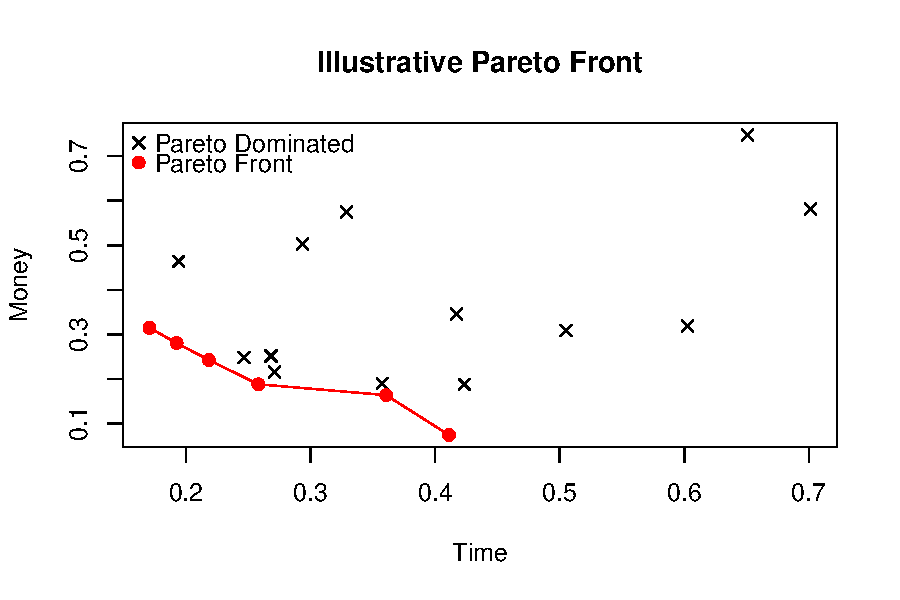
\includegraphics{fig-optim/pfront.pdf}
 \caption{An illustrative Pareto front for a collection of decisions. In this example, smaller values of the attributes Time and Money are preferred. The Pareto front is depicted by the red dots, which are connected by the red line, and consists of decisions for which no other decision offers smaller values of Time \textit{and} Money. The decisions which are Pareto Dominated are illustrated by black crosses. Any decision which is above/to the right of the Pareto front is a Pareto Dominated decision. \label{Fig:pfront}}
\end{figure}

A Pareto front is useful when we want to optimise multiple competing objectives, but it is not entirely clear how objectives compete. If the DM can settle on a utility function to express their preferences, the expected utility surface can (in theory) be maximised. When the utility function depends on the outputs of an expensive and stochastic simulator, maximisation in practice is incredibly difficult. BayesOpt methodology is well developed and can be used to find an approximate maximiser. However, there is only a relatively small amount of work on quantifying uncertainty about the optimal decision. A promising approach borrows ideas from the History Matching (HM) literature \citep{Lawson2016}.

\section{History matching}

HM is a procedure used to identify parameter settings of for a simulator which are consistent with observations from the corresponding physical system \citep{Craig1997, Domingo2020}. \correction{Suppose we have observed data $\by$, are able to specify a bounded domain $\bX \subset R^k$ of simulator inputs, and wish to infer parameters $\bx$ of a model,} statistical or otherwise, $y(\cdot)$.

The usual Bayesian and frequentist inference procedures aim to identify values of $\bx$ which best match $\yobs$, the observed data. This rests on the assumption that data $\yobs$ could be generated from the physical process which the simulator, $y(\cdot)$, aims to mimic. HM allows for many structures for $\yobs$. The nature of the work in this thesis means we only consider $\yobs \in \R$. HM addresses a more critical question than inference; are there \textit{any} values of $\bx \in \calX$ which are consistent with $\yobs$? As a corollary, if there are values of $\bx$ which are consistent with the observed data (allowing for various sources of uncertainty) then the HM toolkit allows us to find these values. These values are referred to as ``Not Ruled Out Yet'' (NROY). Let us consider an illustrative example. Consider the following simulator
\begin{equation}
 y(x) = 0.6 \sin (2 \pi x) + 2 \cos (3 \pi x) + \sin (4 \pi x) + 2x + \varepsilon^{*}, \, x \in [0,1] \label{Eq:hm-toy-fn}
\end{equation}
where $\varepsilon^{*} \sim \mathcal{N}(0,1)$ is an error term to account for all possible sources of uncertainty. Note that the deterministic part of \cref{Eq:hm-toy-fn} is identical to \cref{Eq:example-function}. We later decompose and discuss sources of error and uncertainty. This simulator is tractable and simple, we use this in place of a computationally expensive and complex simulator. Now suppose that we have observed the value $y = 2.5$ from the corresponding physical system. A frequentist could find the best input, $\hat{x}$, by minimising MSE or by specifying and maximising an appropriate likelihood function. Minimising MSE leads to one solution; $\hat{x} = 0.647$. The lack of uncertainty quantification about appropriate values of $\bx$ is a concern.

Uncertainty quantification is at the heart of Bayesian inference thus is a promising alternative. A Bayesian would specify their prior $x \sim \pi(x)$ then perform the usual Bayesian update. Since $y(\cdot)$ is thought to be complex, no conjugate form will exist thus a numerical scheme such as MCMC will be used, possibly assisted by a surrogate. Using Stan \citep{stan} and adopting the prior $x \sim \mathcal{U}(0,1)$ we constructed an MCMC sampler. The MCMC sampler aimed to obtain $10^4$ un-autocorrelated draws. With a burn in period of $10^8$ iterations, a further $10^8$ iterations were performed and thinned by a factor of $10^4$ to obtain $10^4$ draws from $\pi(x \mid y)$. Observing the histogram of posterior samples \correction{(right hand sub-figure of \cref{Fig:mcmc-chain}). The two} modes are centred on the two local maxima of $f(\bx)$, thus the posterior densities seem reasonable. However, the trace plot (left hand sub-figure of \cref{Fig:mcmc-chain}) appears to be `sticky' suggesting that inferences are not completely reliable and the lag $1$ autocorrelation is $0.919$. This is a common computational problem in Bayesian inference, despite our extensive thinning and burn-in periods.

Although we have experienced computational issues, which could be solved by running the Markov chain for a very long time, the Bayesian approach has an interpretation issue which is larger than any computational problem. What exactly does a prior, or posterior density, mean when trying to deduce appropriate decisions? Further, neither the likelihood nor posterior density are telling us which candidate decisions are sensible, given all biases and uncertainties. Allowing for biases and uncertainties within emulator assisted calibration frameworks is well understood \citep{Ohagan01, Goldstein2009} but if there is serious simulator-reality discrepancy, this may be due to a combination of misspecification of the underlying science, an error in the code or poor choice of tuning parameters in numerical solvers. Ultimately, this application of Bayesian inference does not tell us how to make sensible decisions under uncertainty.
\begin{figure}
 \centering
 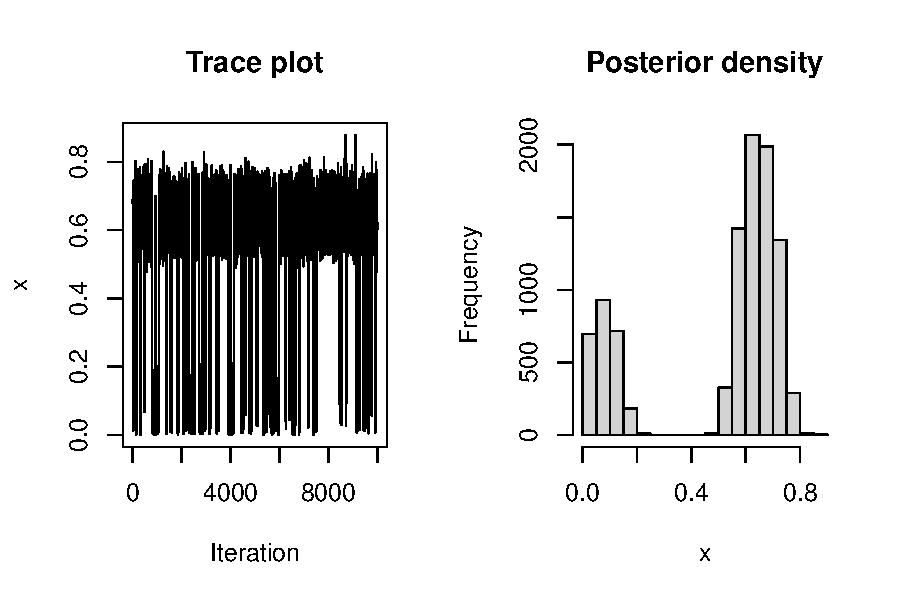
\includegraphics{fig-optim/trace-and-density.pdf}
 \caption{Trace plot (left) and posterior draws (right) from an MCMC sampler to infer appropriate value of $x$ in the illustrative example. \label{Fig:mcmc-chain}}
\end{figure}
\subsection{How can history matching help?}
HM finds appropriate simulator inputs based on how close $\E\{y(\bx)\}$ is to observed data $\yobs$, relative to all uncertainties that the DM is willing to consider. What we want to do is find decisions (parameters) which give an expected utility (simulator output) which is close to the maximum expected utility (observed data), whilst allowing for various uncertainties. These uncertainties may include the uncertainty in the utility function, which is characterised by the emulator, the uncertainty in the maximum expected utility and the uncertainty in the utility function and any simulators which feed into the utility function.

HM is based on a `best input' approach \citep{Ohagan01, williamson2013a}. Suppose that there exists a `best input' (or optimal decision) $\bx^{*}$ such that
\begin{equation}
 \yobs = y(\bx^{*}) + \varepsilon
\end{equation}
where $\varepsilon$ is an error term independent of $\bx^{*}$ and $y(\cdot)$. \correction{The goal of history matching is to find inputs that return outputs which are ``close'' to $y(\bx^{*})$, relative to all the uncertainties in the problem that we are willing to specify.} An implausibility measure, $I(\bx)$, is used to describe how appropriate $\bx$ is for data $\yobs$. Since most common emulation methods (GPs or Bayes linear methods) use expectations and variances for prediction and uncertainty quantification, implausibility measures often have the form in \cref{Eq:default-implausibility}.
\begin{equation}
 I(\bx) = \frac{| \yobs - \E \{y(\bx)\}|}{\sqrt{\var \{\yobs\} + \var\{y(\bx)\} + \var\{ \varepsilon_{\text{MD}} \} }} \label{Eq:default-implausibility}
\end{equation}
where $\varepsilon_{\text{MD}}$ is a mean-zero error-like term which accounts for model discrepancy. \correction{Structured model discrepancy has not been included in \cref{Eq:default-implausibility}. Where appropriate, structured model discrepancy could be removed via the numerator of the given implausibility function.} This proposed implausibility measure is well suited to simulators with a single output. Multivariate implausibility measures have also been proposed and are usually based on the Mahalanobis distance or by specifying an implausibility function for each simulator output, $I_j(\bx)$, and taking $I(\bx) = \max_j I_j(\bx)$. The Mahalanobis distance deems an input as implausible if, jointly, the set of outputs is unusual. The maximum implausibility approach deems an input as implausible if at least one of the outputs is unusual. Both types of multivariate implausibility have been shown be effective in practical examples \citep{Vernon2010,Williamson2017}.

We consider $\bx$ to be an appropriate value, termed `not implausible', when $I(\bx) < I_0$. Often $I_0 = 3$. This value stems directly from Pukelsheim's $3\sigma$ rule \citep{Pukelsheim1994}. The $3\sigma$ rule states that, if $Z$ follows a unimodal, continuous distribution with $\E(Z) = \mu < \infty$ and $\var(Z) = \sigma^2 < \infty$ then
\begin{equation}
 \p \left( | Z-\mu | \geq 3\sigma \right) < 0.05. \label{Eq:pukelsheim}
\end{equation}
Thus using the $3\sigma$ rule means we incorrectly rule out a value of $\bx$ no more than $5\%$ of the time. Pukelsheim actually proved a slightly tighter bound than this, but $\p ( |Z - \mu| \geq 3\sigma ) \leq 4/81 \approx 0.04938$ fails to roll off the tongue so smoothly. If we are to make distributional assumptions about $f(\cdot)$ and $\yobs$, we can make this bound tighter. In the Gaussian case, it is well known that approximately $5\%$ of values lie outside of $\mu \pm 2 \sigma$ and fewer than $1\%$ of values lie outside of $\mu \pm 3\sigma$. Using the $3\sigma$ rule even when probabalistic assumptions are made about $y(\cdot)$ may offer some robustness to misspecification of such assumptions. This is not the only form of implausibility function; any function which suitably measures the difference between the data and the simulator output, relative to all sources of uncertainty is a candidate implausibility function. For example, \citet{Wang2018} use $p$-values to quantify implausibility.

Returning to \cref{Eq:default-implausibility}; $\E\{y(\bx)\}$ and $\var \{ y(\bx) \} $ are critical to many applications of HM. These expectations and variances may be the true mean and variance of $y(\bx)$ when the moments are known. If $y(\bx)$ is intractable, then these can be replaced with the posterior (or adjusted) mean and variance of $y(\bx)$; the inclusion of emulators into the HM framework is natural.

A graphical implementation of HM is given in \cref{Fig:example-hm-graph}. Here we have emulated $y(\cdot)$ and assumed that $\var\{\varepsilon\} = 0.75$, $\var\{\yobs\} = 0.25$ and further assumed $\var\{\varepsilon_{\text{MD}} \} = 0$ (i.e. the simulator is a perfect representation of the physical system). We see that using a cutoff of $3$, some regions of the input space are incompatible with the data. The green regions of the right hand plot of \cref{Fig:example-hm-graph} represent the (wave $1$) NROY space. A mathematical description of this space is
\begin{equation}
 \calX_{\text{NROY}} = \{ x \in \calX : I(x) < I_0 \}
\end{equation}
where we have chosen $I_0 = 3$, justified by Pukelsheim's $3\sigma$ rule.
\begin{figure}
	\centering
	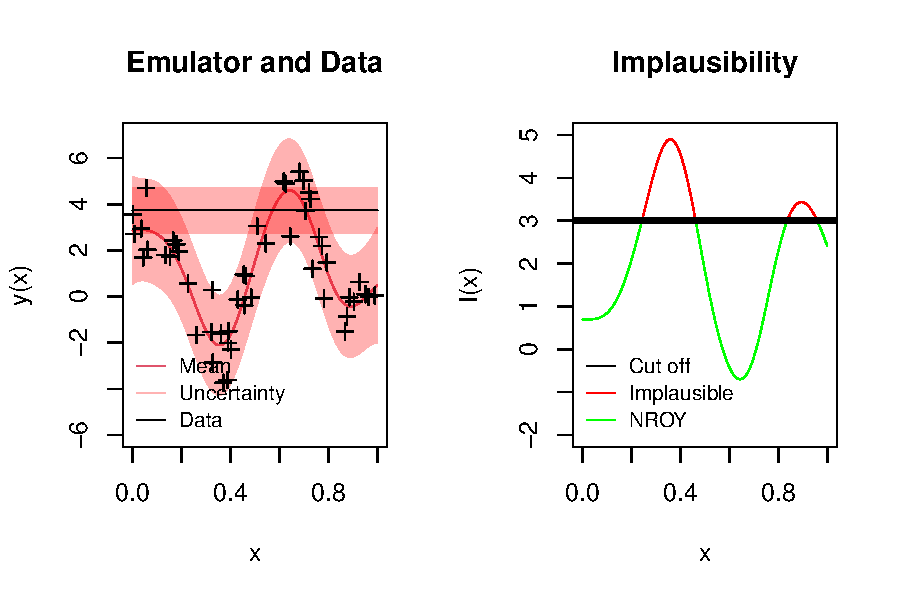
\includegraphics{fig-optim/implaus1.pdf}
	\caption{Illustrative HM procedure for the simulator given in \cref{Eq:hm-toy-fn}. The left hand plot shows an emulator, whose training data are the black `$+$' symbols and $\yobs$ is given as the black horizontal line. The emulator mean has an approximately sinusoidal shape, with pink uncertainty bands about the observed data as well as the emulator. The right hand plot shows the corresponding implausibility function which is colour coded. The red parts of the function ($I(x) \geq 3$) correspond to implausible values of $x$ whilst green regions ($I(x) < 3$) correspond to NROY regions. The black line is the cut off; $I(x) = 3$. \label{Fig:example-hm-graph}
}
\end{figure}
This first wave of HM has led to $34.2\%$ of the original space being ruled out as inconsistent with $\yobs$. HM is well suited to sequential analysis. We can construct new emulators in the NROY space. These new emulators should have reduced uncertainty about them because emulators typically exhibit reduced uncertainty in regions where simulator runs are dense. Since this is an illustrative example, we construct one emulator over the entire NROY space, which is the union of three distinct sub-spaces. When the NROY space is a union of two, or more, disjoint subsets of $[0,1]$, it may be advantageous to construct an emulator on each disjoint subset. This will result in faster matrix calculations. Matrix multiplication is typically $\mathcal{O}(n^2)$ and inversion is typically $\mathcal{O}(n^3)$, now $a(n^k) < (an)^k$ for $a, k > 1$ thus if we have $a$ distinct regions, emulation will be faster if we construct distinct emulators over each distinct region. If the function is non-stationary (which is often the case, but computationally complex to implement over a non-disjoint spaces), allowing for different parameters in different regions of the input space should produce emulators which are a better representation of $y(\cdot)$ \citep{Gramacy2008}.

A second wave of runs was produced. This second wave of runs and emulation allowed us to rule out a further $13.4\%$ of the remaining space. The revised NROY space is now $57\%$ of the original space. We see that each of the two NROY regions in \cref{Fig:example-hm-graph2} corresponds to a neighbourhood around each of the two local modes of $f(\bx)$ since $\yobs = \max f(x)$.
\begin{figure}
 \centering
 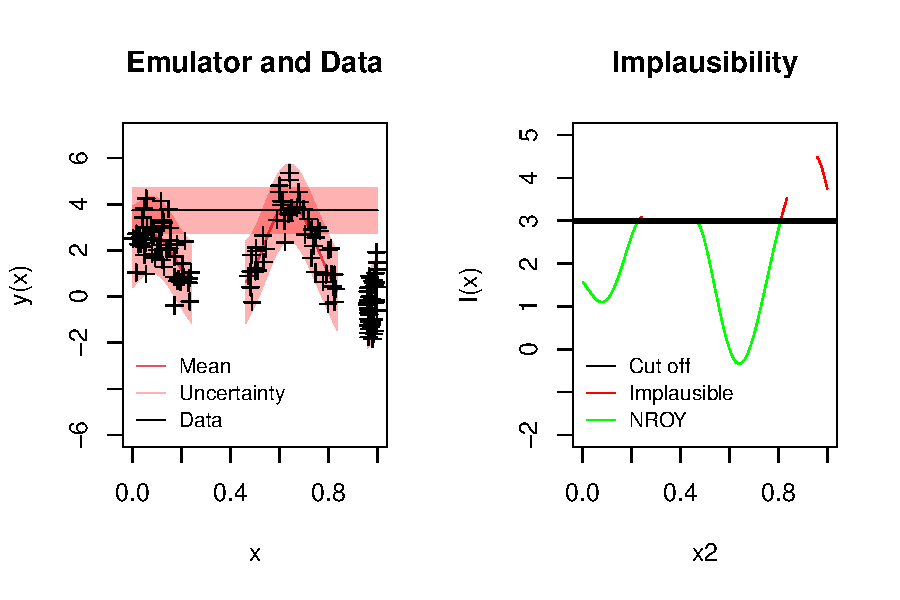
\includegraphics{fig-optim/implaus2.pdf}
 \caption{Illustrative wave $2$ HM procedure for the simulator given in \cref{Eq:hm-toy-fn}. The left hand plot shows an emulator, whose training data are the black `$+$' symbols; $\yobs$ is given as the black horizontal line. The emulator has an approximately sinusoidal shape, with pink uncertainty bands about the observed data as well as the emulator. The right hand plot shows the corresponding implausibility function which is colour coded. The red parts of the function ($I(x) \geq 3$) correspond to implausible values of $x$ whilst green regions ($I(x) < 3$) correspond to NROY regions. The black line is the cut off; $I(x) = 3$. Gaps in both graphs represent the space ruled out after the first wave of HM. These are automatically ruled out at this stage, thus are not considered. }
 \label{Fig:example-hm-graph2}
\end{figure}
 In this instance, we generated inputs uniformly from each sub-region of the NROY space and allowed an equal number of samples in each sub-region. Because this is a one dimensional problem, it is easy to identify the NROY space by inspection. For higher dimensional problems, the only way to identify the NROY region is by evaluation of the implausibility function \citep{Williamson2013}. This is due to the black-box nature of emulators. When multiple waves of emulators have been produced, we may have to evaluate many implausibility functions. If we have performed $k$ waves of emulation, the wave $k+1$ space is given by
\begin{equation}
 \calX_{k+1} = \{ \bx \in \calX_k : I^{k}(\bx) < I^k_0 \}
\end{equation}
where $I^k(\cdot)$ is the wave $k$ implausibility function and $I^k_0$ is the wave $k$ cut off. Note that $k$ here is a superscript and not an exponent. This recursive definition means we \textit{might not} have to evaluate all $k$ implausibility functions to know if $\bx \notin \calX_{k+1}$. Since this requires multiple matrix calculations, this can become computationally costly. To speed up the computation, we should start by evaluating $I^1(\bx)$, then $I^2(\bx)$ and so on. If any $I^j(\bx) \geq I^j_0$, then we should stop evaluation of further implausibility functions since $\bx$ has been ruled out.

Adapting HM to optimisation is a promising tactic when an analyst wants to perform decision support. HM provides a solution to the problem of constructing an interpretable set of decisions which are acceptable, whilst allowing for all relevant uncertainties and biases. The interpretation here is that these decisions are within a given tolerance of the current best decision. This also allows for uncertainty about the best decision seen so far, as, when $y(\cdot)$ is stochastic, there will typically be uncertainty about $U(\bx)$. The analyst can then report $\calX_{k+1}$ to the decision maker; it represents a set of decisions which are not clearly worse than the reported optimal decision, given all the uncertainties considered.
\subsection{Drawbacks of HM}
\correction{HM is not a perfect approach, there are potential drawbacks that we should be aware of.}

\correction{The first potential drawback is that, once a point has been deemed NROY, it is NROY for all future waves. This means, if we were to rule out $\bx^{*}$, no future waves would contain the optimal decision, or best input, as appropriate.}

\correction{Another potential drawback is that, at the number of waves grows, we are increasingly likely to rule out good points. The error rate for a history matching is often defined at the wave-level. Over multiple waves of HM, the proportion of incorrectly ruled out points is compounded. For a large number of waves, this means we are in danger of ruling out large regions of the input space that leads to good decisions, or is compatible with observed data.}

\correction{A third drawback is that characterising the NROY space is achieved by random sampling. This means, it is not possible to fully understand the NROY region. For example, if a sampling scheme used to describe the NROY space missed a disconnected region of the NROY space, we might not know. In practice it is hard to tell if disconnected regions exist, and even harder to tell if we have captured all of them.}

\subsection{HM for decision support}
When using HM techniques for optimisation or decision support, the implausibility measure used must be different from \cref{Eq:default-implausibility}. This is because, (i) we have not observed data from a physical system and (ii) the modulus operation in the numerator will cause problems if the emulator predicts a value larger than the current largest value. Recall that the goal is to maximise $f(\bx)$, thus, within decision support, authors typically use an implausibility measure of the form
\begin{equation}
 I(\bx) = \frac{y^* - \E \{f(\bx)\} }{\sqrt{ \var\{y^*\} + \var\{f(\bx)\} + \var\{\varepsilon_{\text{MD}}\}}}.
\end{equation}
\citet{Owen2020} uses this implausibility function but set $I(\bx) = 0$ whenever $\E\{ f(\bx) \} > y^{*} $. \citet{Baker2020c} retains the exact value of $I(\bx)$ to communicate which decisions are much likely to be better than our reference value. If $I(\bx) \leq -3$, then $\bx$ is `ruled in' as a good candidate decision, since it is much larger than the reference value $y^{*}$. The $\bx$ satisfying $I(\bx) \geq 3$ are ruled out, as is standard. Then, the next wave is constructed in the range for which $|I(\bx)| < 3$ to allow the analyst to explore the decisions for which it is not clear if they are acceptable or not.
\begin{figure}
 \centering
 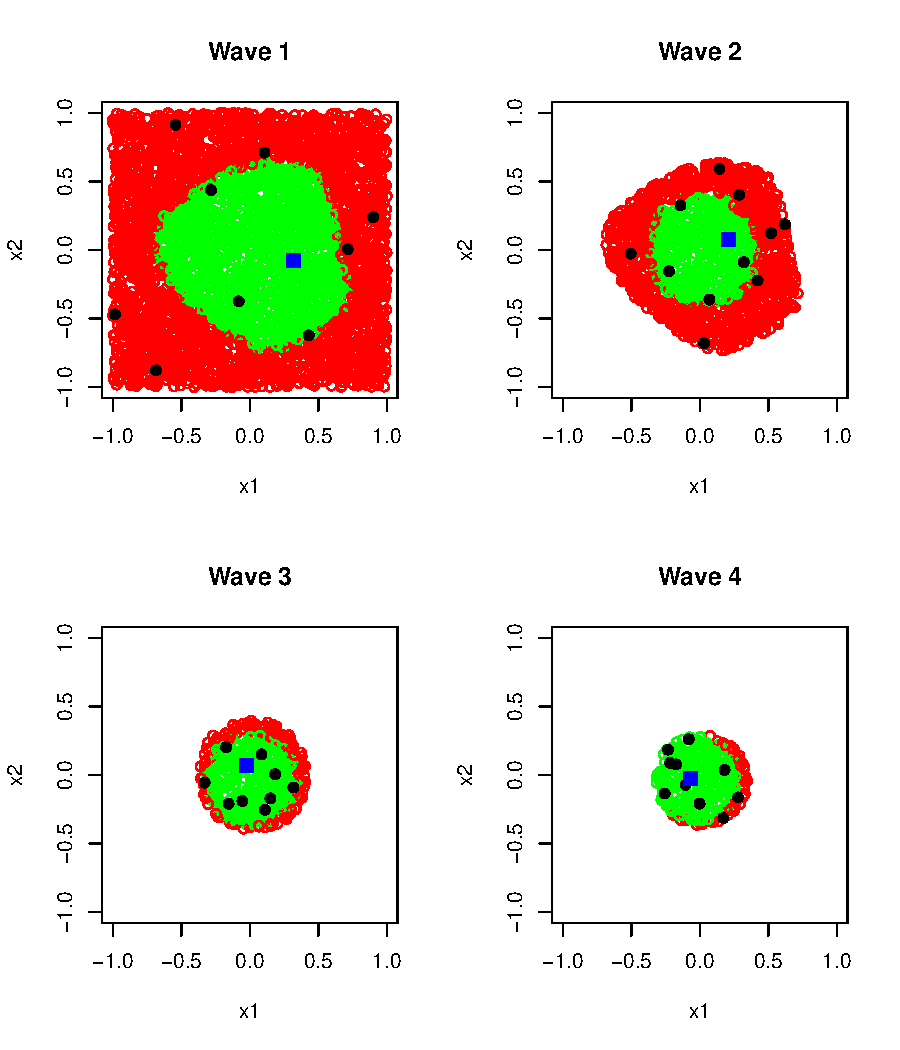
\includegraphics{fig-optim/quad-optim.pdf}
 \caption{An illustrative example of using HM inspired techniques to construct a set of good decisions under uncertainty. The circles are a large set of candidate decisions; red circles denote decisions that have just been ruled out ($I^k(\bx) \geq 3$) whereas green decisions are those which are NROY ($I^k(\bx) < 3$). Black dots are design points for the wave $k$ emulator with the blue square being the design point with largest expected utility at wave $k$. \label{fig:quad-optim}}
\end{figure}
An illustrative example of iterative HM inspired decision support is given in \cref{fig:quad-optim}. This method of fitting a sequence of emulators (not to be confused with sequential design\footnote{It could be argued that iterative refocussing is a batch-sequential design where the size of the batches is much larger than the number of batches.} like BayesOpt or ALM) is sometimes termed ``iterative refocussing'' as the NROY space focuses in on a smaller region after each wave of emulation/HM \citep{Williamson2017, Volodina2021}. Here we are trying to optimise a utility function $U(\bx) = 2 - x_1^2 - x^2_2$ but the observations are noisy; $y(\bx) \sim \mathcal{N}(U(\bx), 0.1^2)$. We specified a model discrepancy variance of $\var\{\varepsilon_{\text{MD}}\} = 10^{-6}$.

Each wave of emulation allows us to concentrate simulator runs on regions of the input/decision space which typically produce larger values of $U(\bx)$. This allows for improved decision making because the expected utility values are usually increasing. Also the emulators become more accurate within the NROY region as it shrinks; this means that the emulator mean response at later waves typically becomes a more accurate representation of $U(\bx)$. Although the NROY volume shrinks, due to the reduction in $\var\{f(\bx)\}$, $\var\{\varepsilon_{\text{MD}}\}$ is a limiting factor in the reduction of the NROY space, and to some extent the uncertainty about the optimal decision, $\var\{U^{*}\}$ will also be a limiting factor (in principle, this will shrink to $0$ as the number of runs grows, but runs are expensive thus limited). This means that, eventually, iterative refocussing will lead to diminishing returns. We have illustrated the diminishing returns in \cref{fig:nroy-numbers}; the volumes shown in these two sub-figures correspond to the NROY volumes in each sub-figure of \cref{fig:quad-optim}. We see that the size of the NROY volume decreases drastically in the first two waves of emulation, but the latter two waves lead to more modest reductions in the number of NROY decisions. This is explained by $\var\{ f(\bx) \}$ reaching a small value. After each wave of emulation, the average value of $\var\{f(\bx)\}$ within the NROY regions $\calX_2$ through to $\calX_5$ is $(1.79, 0.35, 0.087, 0.14)\times 10^{-2}$. After each of the first three waves of emulation, the average variance typically decreases by a significant fraction. The final wave leads to a slight increase in the average variance. This is likely a random artefact of the sample, the final average variance is of similar size to the third, and the reduction in the NROY volume is small, which suggests we should terminate the HM procedure.
\begin{figure}
 \centering
 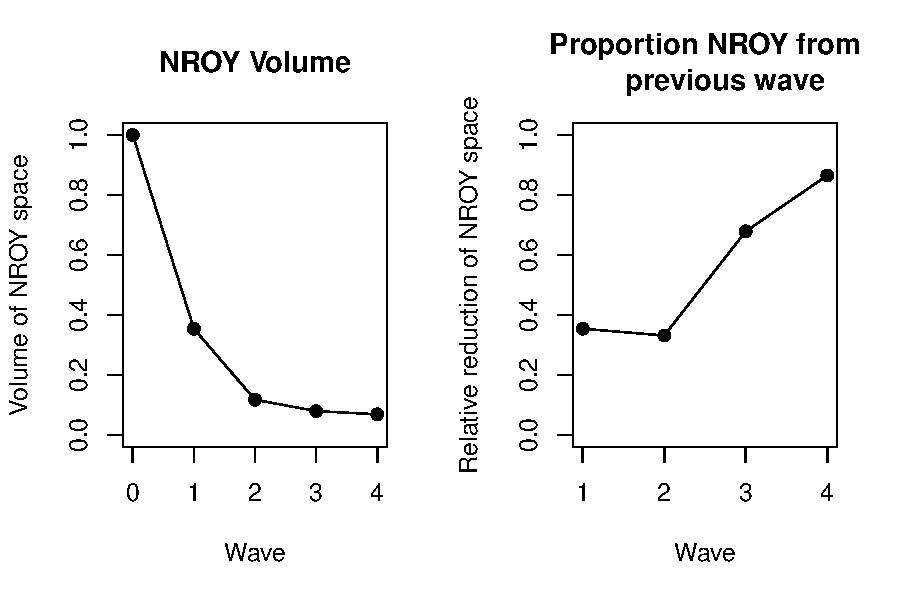
\includegraphics{fig-optim/nroy-reduction.pdf}
 \caption{Graphs depicting how the volume of the NROY region shrinks as the number of waves increases. The left hand plot shows the ratio $|\calX_{k+1}|/|\calX|$ which is the proportion of NROY decisions remaining after $k$ waves of emulation and HM; we see the first two waves lead to larger reductions in the NROY volume than the latter waves. The final wave of emulation leaves us with just $7\%$ of the original space as NROY. The right hand plot shows $|\calX_{k+1}|/|\calX_k|$, that is, the proportion of decisions that are NROY after wave $k$ that are also NROY at wave $k+1$. The right hand plot shows that the second wave was, in some sense, slightly more effective than the first wave. However the $4$th wave of emulation only ruled out $13\%$ of points in $\calX_4$, which is small thus the HM procedure was terminated. The $0$th `wave' denotes all the initial volume (prior to emulation/HM).\label{fig:nroy-numbers}}
\end{figure}

\subsubsection{How does HM address exploration versus exploitation?}

In BayesOpt, we can analyse the exploration-exploitation trade-off by studying acquisition functions. For HM inspired techniques we take a less technical approach to arguing that HM satisfies the trade-off.

During each wave of HM, we construct a design in $\calX_{k+1}$ which is, in part, based on an implausibility measure. The measure is of the form
\begin{equation}
 I_{k+1}(\bx) = \frac{y^{*} - m^{*}(\bx)}{ \sqrt{v^{*}(\bx) + k} }
\end{equation}
where $k$ represents other sources of uncertainty such as model discrepancy. Clearly, if $m^{*}(\bx)$ is large, then $I_{k+1}(\bx)$ will be small. Similarly, if $v^{*}(\bx)$ is large, $I_{k+1}(\bx)$ will also be small. We retain $\bx$ for future study when $I_{k+1}(\bx)$ is small. Exploitation is achieved in two ways; firstly, by reversing the previous argument, when $m^{*}(\bx)$ and $v^{*}(\bx)$ are both small, we will not retain $\bx$ at the next wave. This effect applies to previous waves also. We are only considering points which have previously been identified as promising or uncertain, thus we are exploiting knowledge from previous waves of emulation.

Some additional exploration, which is not present in BayesOpt, can be achieved via $k$. Large values of $k$, corresponding to larger model discrepancy and/or other sources of uncertainty, typically lead to larger NROY spaces. This means we consider a larger volume of decisions at later waves. Further, since the HM inspired approach reports uncertainty about the best decision seen so far, once we have terminated the HM procedure there is more exploration to be done. The decision maker themselves must consider decisions which are still NROY to settle on a final decision.


\subsection{Wave $k>1$ designs}

A design is required for each wave of emulation. In wave $1$, LH sampling is the usual approach due to the space filling properties of LHs. For waves $2$ and beyond, the design space is characterised by the implausibility measure. The resulting NROY space has no obvious form when expressed as a function of $\bx$, this is seen in \cref{fig:quad-optim}. Although not a rigorous term, `blob shaped' would be a reasonable description. Ultimately the NROY space depends on the posterior mean and variance given by an emulator. Thus the only way to know if $\bx$ is ruled out after $k$ waves of emulation is to evaluate $I^k(\bx)$. This often leads to NROY regions with unusual shapes \citep{Garbunoinigo2020}. As a result of the NROY space being defined in a black-box manner, design for waves $k>1$ can be a challenging task.

The simplest approach to (uniform) design for a wave $k+1$ emulator is rejection sampling. Usually, a large LH is constructed over the original input space and then the points which are NROY after $k$ waves are retained for the wave $k+1$ emulator \citep{Vernon2010}. This approach is reasonably efficient when the NROY space is a relatively large fraction of the original space (say, more than $1\%$ of the original space). When the NROY space is a small fraction of the original space, the approach becomes very expensive. If, after $k$ waves of emulation, $|\calX_{k+1}| = p_k|\calX|$ then if we want $N$ NROY samples we would expect a LH of size $N/p_k$ to give us $N$ NROY samples. This problem is harder in higher dimensional spaces due to the curse of dimensionality and also more computationally expensive when we use non-random LHs (for example, maximin LHs). Another problem with this approach is that it returns a design of a random size. If we know we can perform no more than $N$ runs of the simulator at each wave, we would usually want to perform exactly $N$ runs.

There are promising alternatives to rejection sampling, based on other Monte Carlo schemes. The Monte Carlo schemes all take the same view on the problem. Sampling uniformly from $\calX_{k+1}$ is mathematically equivalent to sampling from the following density
\begin{equation}
 \pi_{k+1}(\bx; I_0) \propto \begin{cases}
  1, & I^k(\bx) < I_0\\
  0, & I^k(\bx) \geq I_0
 \end{cases}.
\end{equation}
 \citet{Williamson2013} use evolutionary Monte Carlo (EMC) and \citet{Drovandi2021} use sequential Monte Carlo (SMC) to construct NROY designs for which the the NROY space is a tiny subset of $\calX$. Another promising approach, which is conceptually much simpler than the EMC and SMC approaches, is slice sampling. Within the HM context, this was first used by \citet{Andrianakis2017a} and the slice sampler for iterative refocussing is simpler than the standard slice sampling algorithm since the density is constant within $\calX_{k+1}$ \citep{Neal2003}.

\subsection{Slice sampling for NROY regions}

We now provide some details of the slice sampling algorithm introduced by \citet{Neal2003}, which is given in \cref{alg:neal-slice} and compare this to the sampler used by \citet{Andrianakis2017a}, which we describe in \cref{alg:nroy-slice}. We will aim to sample from a density $\pi(\bx)$ which is only known up to proportionality; $\pi(\bx) = k \varphi(\bx)$ where $k^{-1} = \int \varphi(\bx) \, \diff \bx$ is an intractable normalisation constant. A version of the algorithm proposed by \citet{Neal2003} is given in \cref{alg:neal-slice}, and a corresponding illustration for a univariate example is given in \cref{Fig:slice-diagram}, where $\varphi(\bx)$ is a linear combination of three univariate Normal densities. The vertical blue line denotes our initial sample, $x_0$, and the horizontal blue line denotes $\varphi(x_0)$. The horizontal red line represents the horizontal slice $y_0 \sim \mathcal{U}(0, \varphi(x_0))$ and then the dashed red lines illustrate the sample space for the next sample, $x_1$. A uniform sample along the $x$ axis where red dashed lines are present gives us our next draw from $\pi(x)$. Slice sampling is a powerful sampling technique because we only need to be able to (i) sample uniformly and (ii) solve equations (construct the horizontal slice). The equation solving aspect can be challenging. Our illustrative, one-dimensional example had four roots to find. In a complex high dimensional problem, we may not know how many roots exist.

The standard slice sampler (\cref{alg:neal-slice}) differs somewhat from the slice sampler for NROY regions (\cref{alg:nroy-slice}). A similarity between the two is that they are both component wise; each element of $\bx$ is updated one-by-one. Some steps in the standard slice sampler are not required for generating samples from the NROY region. The first difference is that in \cref{alg:nroy-slice} we do not calculate $\varphi(\bx_0) = \mathbb{I}(\bx_0)$ because we know it is $1$. Secondly, we do not sample $y_0 \sim \mathcal{U}(0, \varphi(\bx_0))$ because $\varphi(\bx)$ is either $0$ or $1$. Any NROY sample satisfies $\mathbb{I}(\bx \in \calX_{k+1}) = 1$, therefore $y_0=1$ in all cases. This bypasses the tricky root finding problem.

Slice sampling, as in \cref{alg:nroy-slice}, allows us to update the $i$th input. The slice sampling can be made drastically more efficient by changing the limits of the uniform proposal. If it is known that $\calX_{k+1} \subseteq [l_1, r_1] \times [l_2, r_2] \times \ldots [l_m, r_m]$ then we can replace the $\mathcal{U}(0,1)$ random sample with a $\mathcal{U}(l_i, r_i)$ sample, where $0 \leq l_i < r_i \leq 1$. This efficiency gain may come at a cost: if an $l_i$ or $r_i$ are misspecified, we would neglect parts of the NROY space. For input $i$, suppose $l_i$ is chosen to be too large, then any $\bx \in \calX_{k+1}$ such that $x_i < l_i$ would never be sampled.
\begin{figure}[h]
 \centering
 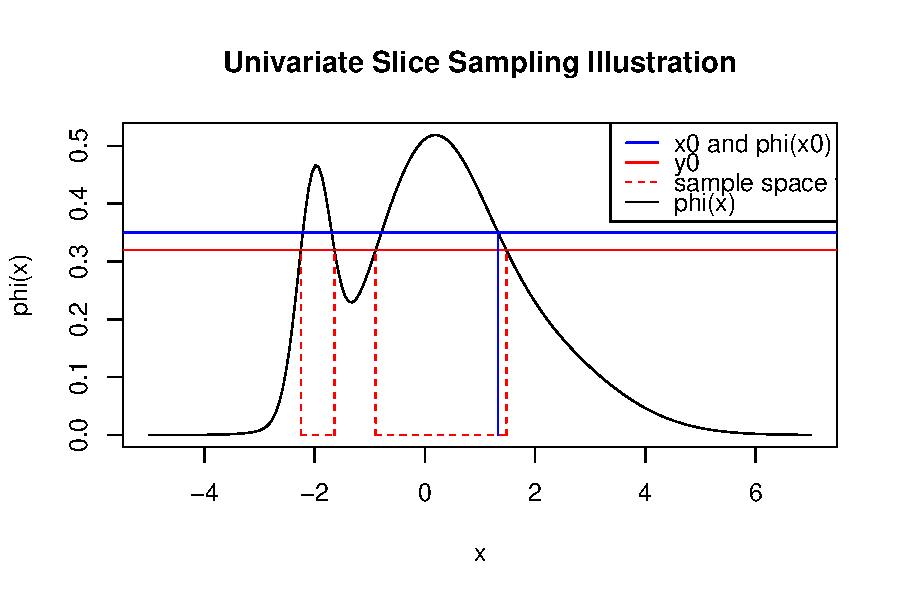
\includegraphics{fig-optim/slice-diagram.pdf}
 \caption{An illustration of how to sample $x_1 \sim \pi(x)$ given a draw $x_0 \sim \pi(x)$ when the only information we have about $\pi(x)$ is that $\pi(x) \propto \varphi(x)$. The black curve represents $\varphi(x)$, the vertical blue line represents $x_0$, the initial sample and the horizontal blue line represents $\varphi(x_0)$. The horizontal solid red line represents $y_0 \sim \mathcal{U}(0, \varphi(x_0))$. The dashed red lines denote the space in which $x_1$ is uniformly sampled from to obtain a new draw from $\pi(x)$.\label{Fig:slice-diagram}}
\end{figure}
\begin{algorithm}[h]
\caption{A single iteration of a generic, component-wise slice sampler, based upon the slice sampler presented by \citet{Neal2003}. \label{alg:neal-slice}}
\begin{algorithmic}
\Require A density known up to proportionality $\pi(\bx) \propto \varphi(\bx)$, an initial sample $\bx_0 \sim \pi(\bx)$ where $\bx_0$ is an $m$ dimensional parameter vector.
\State $\bx_1 \gets \bx_0$
\For{$i = 1$, $2$, $\ldots$, $m$}
 \State $\varphi_0 \gets \phi(\bx_0)$ and sample $y_0 \sim \mathcal{U}(0, \phi_0)$
 \State Find the set $\tilde{\calX} = \{x_i : \varphi(x_i, \bx_{-i}) \geq y_0 \}$
 \State Draw $\tilde{x}_i \sim \mathcal{U}(\tilde{\calX})$\Comment{Sample uniformly from $x \in \tilde{\calX}$}
 \State Set $x_{1,i} \gets \tilde{x}_i$ \Comment{Update the $i$th component of $x_0$}
\EndFor
\State Return, $\bx_1$, the new sample from $\pi(\bx)$.
\end{algorithmic}
\end{algorithm}
\begin{algorithm}[h]
\caption{A single iteration of a component-wise slice sampler used for sampling from NROY regions, based upon the slice sampler presented by \citet{Andrianakis2017a}. \label{alg:nroy-slice}}
\begin{algorithmic}
\Require An indicator function $\mathbb{I}(\bx \in \calX_{k+1})$ for identifying inputs which are NROY, an initial NROY point $\bx_0 \in \calX_{k+1} \subseteq [0,1]^m$ where $\bx_0$ is an $m$ dimensional parameter vector.
\State $\bx^{*} \gets \bx_0$
\For{$i = 1$, $2$, $\ldots$, $m$}
 \State $I^{*} \gets 0$ \Comment{Initialise an indicator variable}
 \While{$I^* \neq 1$}
  \State Draw $x_i \sim \mathcal{U}(0,1)$ \Comment{Change the $i$th input}
  \State $x^{*}_i \gets x_i$
  \State $I^{*} \gets \mathbb{I}(\bx^{*} \in \calX_{k+1})$ \Comment{Evaluate the implausibility measure at the new input}
 \EndWhile
 \State $\bx_1 \gets \bx^{*}$ \Comment{Update the $i$th component of $\bx_0$}
\EndFor
\State Return, $x_1$, the new sample from $\pi(\bx)$.
\end{algorithmic}
\end{algorithm}
\correction{
However, \cref{alg:nroy-slice} has an issue: in general, it is not \textit{ergodic}. That is, it may not be possible to fully explore $\calX_{k+1}$ with a single run of the algorithm. This can be amended by repeating the algorithm for many initial points $\bx_0$ which are randomly chosen (for example, by sampling uniformly in $[0,1]^m$ until we find an NROY point).}

We formalise this in \cref{alg:ergodic-slice}.

\begin{algorithm}[h]
\caption{An ergodic variant of \cref{alg:nroy-slice}. \label{alg:ergodic-slice}}
\begin{algorithmic}
\Require An indicator function $\mathbb{I}(\bx \in \calX_{k+1})$, a number of replications, $R$, a required number of samples, $n =  n' \times R$, and a function $\texttt{slice\_sampler\_one\_step}(\mathbb{I}(\bx \in \calX_{k+1}), \bx_0)$ which takes an implausibility function, $\mathbb{I}(\bx \in \calX_{k+1})$ and an NROY point, $\bx_0$ and returns a new NROY point.

\For{$r = 1, 2, \ldots, R$}
  \State {$I_r \gets 0$}
  \State Initialise a matrix $X_r$ with $m$ columns and $n'$ rows
  \While{$I_r \neq 1$}
    \State $\bx_{1, r} \gets \mathcal{U}([0, 1]^m)$
    \State $I_r \gets \mathbb{I}(\bx{1, r} \in \calX_{k+1})$
  \EndWhile
  \For{$i = 2, 3, \ldots, n'$}
  \State $\bx_{i, r} \gets \texttt{slice\_sampler\_one\_step}(\mathbb{I}(\bx \in \calX_{k+1}), \bx_{i-1, r})$
\EndFor
\EndFor
\State Collect all $X_r$ into a single matrix $X$, with $m$ columns and $n$ rows.
\State Return $X$, the collection of NROY samples.
%\Return $X$, a sample of $n$ NROy points.
\end{algorithmic}
\end{algorithm}

\section{Discussion}

This chapter has reviewed methods for decision making under uncertainty to prepare us for the next chapter, in which we solve a decision problem using some of the illustrated techniques. We began by considering decision making as an optimisation problem. We discussed that although mathematically well defined, decision making is a difficult task. The difficulty of the problem is increased when we have limited understanding of $U(\bx)$ due to the stochastic, expensive and gradient-free nature of many simulators.

We discussed various optimisation methods, then settled on Bayesian Optimisation as being an efficient and effective approach to \textit{decision making} with complex models. We discussed various acquisitions functions and presented decision theoretic justifications for each acquisition function, where relevant. A consequence of using BayesOpt for decision making is that it makes decisions on behalf of the DM, which poses questions about \emph{who} is making decisions. We argue that viewing complex, ill-defined problems as those possessing a single, optimal solution is myopic. An appropriate approach to addressing these concerns is to use \textit{decision support} to simplify, but not solve, the problem for the decision maker. We discussed the idea of a Pareto front as a decision support tool, however, we are working within a regime where a utility function has been established but is expensive to evaluate. We therefore treat $U(\bx)$ as an unknown function which is optimised under multiple sources of uncertainty. These may include the uncertainty induced by the expensive nature of the utility function, any stochasticity present in simulations, uncertainty about model parameters which are not decision parameters as well as the uncertainty about the elicited utility function.

Therefore, we settled on using HM inspired techniques to iteratively hone in on a set of feasible solutions, called the NROY space. These decisions are a set of solutions, which, given all relevant sources of uncertainty, are not worse than the best decision we have found so far. We briefly discussed some approaches to iterative construction of emulators, and in particular discussed some approaches to the wave $k>1$ design problem. Monte Carlo methods, commonly used to perform Bayesian inference, offered a promising solution to constructing uniform designs across the NROY space. In particular, we advocate for slice sampling as it strikes a good balance of conceptual simplicity, computational simplicity and effective results. The only mechanism we need in addition to the implausibility function is a uniform sampling scheme, and all major scientific computing libraries allow for uniform sampling.

Empirical evidence tells us that these are typically much more efficient than rejection sampling when $|\calX_k|$ is a tiny fraction of $|\calX|$. However, we did not discuss how to get the optimum `reference' value, which is central to the HM inspired approach. In the next chapter, we explore this further and employ a slice sampling approach to construct a set of feasible decisions.
\end{chapter}

  \begin{chapter}{A Decision Support Framework for Offshore Wind \label{Ch:ds-for-ow}}

Consider the problem of storing spare subassemblies, which will replace subassemblies in an offshore wind farm which have suffered a `serious' failure. Spare parts may be stored in a warehouse near to the dock, at which spare parts will be loaded onto a boat so the spare can be shipped out to the turbine to be fitted. This problem has been considered previously in the literature. \citet{Tracht2013} perform a scenario analysis which investigates the effect of limited amounts of spare components and equipment on preventative maintenance. A review of various models used for analysing spare parts strategies is given in \citet{Tusar2022}. The review stresses that not enough work is being done on constructing an optimal combination of spare parts, as once an order has been placed, the time to delivery for spare components can be sufficiently long to reduce availability. We aim to address this. The review suggests most analyses are interested in minimising downtime. Our analysis will consider availability (downtime is essentially the opposite of availability) but we will also consider the costs incurred by increasing availability.

This chapter proposes a decision support framework which is flexible enough to incorporate relevant sources of uncertainty into a decision support exercise. A key difference with our approach, compared to standard approaches, will be that we use ideas from the history matching (HM) and BayesOpt literature to construct a set of sensible decisions. BayesOpt is typically used to find a single decision which is (approximately) optimal, but the BayesOpt routine also provides us with an emulator across the entire decision space, which can be used to construct a set of feasible decisions. Our approach is novel as we will employ ideas from HM to conduct a post-hoc analysis of the BayesOpt routine.

We will begin by outlining competing objectives a DM may consider in an offshore wind setting. We progress to formalising the decision problem and thus translating the decision problem to an optimisation problem. A novel application of BayesOpt and HM techniques then allows us to construct a set of sensible decisions; the DM will be presented with this set and uses it to make a final decision.
\section{The decision problem}

Recall that the Athena simulator models a turbine as being composed of $8$ important subassemblies, and a ninth `catch all' subassembly. They are as follows: 1. gearbox, 2. generator, 3. frequency converter, 4. transformer, 5. main shaft bearing, 6. blades, 7. tower, 8. foundations, and 9. catch all. The DM has two problems to solve simultaneously, whilst aiming to maintain high availability of the wind farm:
\begin{itemize}
 \item[1.] Which warehouse, from a set of candidate warehouses, should the spare parts be stored in?
 \item[2.] What is the best way to manage the warehouse?
\end{itemize}
Good management of a sub-optimal warehouse may be much better than bad management of the optimal warehouse. Of course, we strive for optimal management of the optimal choice of warehouse. The management of the warehouse is broken down into the answers of the following two questions:
\begin{itemize}
 \item[1.] How many spare parts should we store for each subassembly?
 \item[2.] At what point should we buy in more spare parts for the subassembly?
\end{itemize}
%Almost every problem so far in this thesis has been addressed with decision theory. That theme is not going to end on page \thepage.
We therefore need to formulate a utility function over all relevant attributes and specify an appropriate prior distribution over uncertain quantities. We do not directly specify any particular prior distribution; we instead adopt the priors elicited by \citet{Zit2021}. These priors were elicited from practising engineers who are able to give informed assessments of uncertain quantities. We will act as the DM as well as the analyst. In this exercise we will specify the utility function. The utility function will express sensible preferences, but will not represent the preferences of a real DM. We stress that the emphasis of this chapter is the development of an appropriate optimisation/decision support framework, rather than precise details of utility functions or precise details of the problem itself.

\section{Mathematical formulation of the decision problem}
Here we will formulate the decision problem following the elicitation guidelines outlined in \cref{Ch:background}; more details can be found in \citet{Smith2010} or \citet{Keeney1976}. Our problem is to choose a warehouse, $k$, of size $W_k$, and fill the warehouse with spare parts for each of the $9$ subassemblies. We will allocate $s_i$ spares for subassembly $i$. We also need to construct a policy for restoring the numbers of spare parts as they deplete, to ensure smooth running of the warehouse.

We begin by identifying an appropriate set of attributes. We then specify preferences through marginal utility functions, which will be combined into a single multi-attribute utility function. The first stage of elicitation of a utility function is to define all attributes relevant to the problem.

\subsubsection{Relevant attributes}

There are several attributes relevant to this problem. The key attributes are:
\begin{itemize}
 \item The availability time series (performance) of the wind farm.
 \item The choice and cost of the warehouse in which spare parts are stored.
 \item The number of spares of each type of subassembly.
 \item The policy which dictates when to buy in more spare parts.
\end{itemize}
There are many more attributes a DM could consider, but this is sufficient in our case to demonstrate the complexity of the problem and the application of methodology. We would next need to decide what the consequences, $c_i$, of any possible decision would be. The consequences of any decision are given in \cref{Tab:consequences} alongside information about the consequences. For example, the availability time series output by Athena over a $5$ year period is internally processed by Athena and a length $240$ vector is output. We know that this time series is stochastic. The restoration policy is both a decision and a consequence here; the consequence is the set of $p_i$, the thresholds that trigger an ordering for more spare parts of type $i$ as in \cref{Sec:athena-variant}, we would want to leave this as late as possible. The cost of the warehouse could be argued to be stochastic (for example, if the unit is rented, the owner may increase the rent to some uncertain value at some uncertain future time point). We assume, for simplicity, that the cost is fixed and related to its capacity. In \cref{Tab:consequences} we the use notation $\mathcal{S}^k_n$. This represents the $k$ dimensional discrete simplex which we will define as
\begin{equation}
 \mathcal{S}^k_n = \left\{\bx \in \N^{k+1} \,\,\bigg|\, \sum_{i=1}^{k+1} x_i = n, x_i \in \{1, 2, \ldots, n-k+1\} \right\}. \label{Eq:disc-simplex}
\end{equation}
We have chosen to define $\mathcal{S}^k_n$ in this way as it reflects aspects of our application. A warehouse of size $n$ can have a minimum of $1$ spare part of type $i$ and can have at most $n-k+1$ spare parts of type $i$. This is because the other $k-1$ types of component all need at least $1$ spare part. This essentially assumes that all spare subassemblies are of similar shape and size, this is clearly an over simplification which could be addressed in future work.

%decisions
\begin{table}[t]
	\centering
	\begin{tabular}{llll}
		\toprule
  Label & Description & Parameter Space & Stochastic?\\\cmidrule{1-4}
  $c_1$ & Availability time series & $c_1 \in (0, 1)^{240}$& Yes\\
  $c_2$ & Choice of the restoration policy &$c_2 \in (1, 99)^9$& No\\
  $c_3$ & Warehouse size & $c_3 \in \{50, 75, 100\}$& No\\\bottomrule
	\end{tabular}
	\caption{Summary of the consequences of a future decision to be made. These variables cause changes in the stochastic and deterministic consequences and it is the decisions themselves that will form the inputs of a future emulator.	The stochastic column describes how we model the consequence. \label{Tab:consequences}}
\end{table}
%consequences
\begin{table}[t]
	\centering
	\begin{tabular}{lll}
		\toprule
  Label & Description & Parameter Space\\\cmidrule{1-3}
  $x_1$--$x_9$ & Number of spare parts & $x_{1:9} \in \mathcal{S}^{8}_{x_{19}}$\\
  $x_{10}$--$x_{18}$ & Critical Percentages & $x_{10:18} \in (1,99)^9$\\
  $x_{19}$ & Warehouse size (number of parts) & $x_{19} \in \{ 50, 75, 100 \}$\\\bottomrule
	\end{tabular}
	\caption{Summary of the decision variables. These are the variables for which individual utility functions will be elicited, to be combined into an overall utility function. See \cref{Eq:disc-simplex} for the definition of $\mathcal{S}^k_n$.	\label{Tab:consequences}}
\end{table}
Our approach to eliciting the utility function will follow the advice of \citet{Smith2010} and \citet{Keeney1976}. We assume that consequences are mutually utility independent, elicit a marginal utility function for each consequence using probability or certainty equivalents and then combine the marginal utility functions into an overall utility function via a multiplicative or additive form, depending on the preferences of the DM.
\section{The marginal utility functions}
Utility functions are unique up to positive affine transformations. That is, $au(x) + b$ expresses exactly the same preferences as $u(x)$ for any $a > 0$ and $b \in \R$. For this reason, we will construct all utility functions on the unit interval. This also allows for easier elicitation, as utility and probability will be on the same scale.
\subsubsection{Utility of availability}
The availability is a time series. At time $t$, denote the (random) availability by $A(t)$, this will form our first consequence. In particular, the Athena simulator outputs a length $L$ time series, $(A(t_1), A(t_2), \ldots, A(t_{L}))$ at equally spaced intervals. In our analysis, $L = 240$ due to various settings within Athena. We therefore define $c_1(t) = A(t)$ and let $c_1 = (c_1(t_1), c_1(t_2), \ldots, c_{1}(t_{L}))$. The utility of a time series may be time dependent, however, in this problem we will work with the assumption that a given availability has utility which does not depend on time. In other words, if we let $\tilde{u}_1(c_1(t), t)$ be the utility for $c_1(t)$ at time $t$ then $\tilde{u}_1(c_1(t), t) = \tilde{u}_1(c_1(t))$. We would then take the utility of the entire time series to be
\begin{equation}
 u_1(c_1) = \frac{1}{L}\sum_{j = 1}^{L} \tilde{u}_1(c_1(t_j)).
\end{equation}
This is just point-wise utility averaged over time. This average could be weighted if high availability is more important at some time points than others. See \citet{Rios2003} for examples of time-dependent utility elicitation.

We believe a utility function which allows for a varying attitude to risk would be appropriate for $\tilde{u}_1(c_1(t))$. The reason for this is that, for regions of high availability, a DM would be risk-averse, or risk-neutral, in trying to increase availability. However, whenever the availability is very low, we would be risk-seeking in order to ensure the wind farm is viable. An appropriate functional form is:
\begin{equation}
 \tilde{u}_{1}(c) = \beta^{-1} \left\{\frac{(c - a)}{\sqrt{1 + b (c-a)^2}} - \alpha\right\}
\end{equation}
where $a \in (0,1)$ and $b>0$ are parameters to be elicited and $\alpha$, $\beta \in \R$ are scaling parameters which force $0 \leq \tilde{u}_{1}(c) \leq 1$ for any $c \in [0,1]$. $\alpha$ and $\beta$ have the following algebraic forms:
\begin{align}
 \alpha &= -\frac{a}{\sqrt{1 + a^2b}}\\
 \beta &= \frac{1 - a}{\sqrt{1 + b(1-a)^2}} -\frac{a}{\sqrt{1 + a^2b}}.
\end{align}
Now, since we enforce the constraints $\tilde{u}_1(0) = 0$ and $\tilde{u}_1(1) = 1$, we only need to elicit two certainty equivalents to construct a fitted form for $u_1(c)$. To do this, we will use a bisection method. First we specify the availability, $c^{(1)}$, such that $[0, 1; 0.5] \sim c^{(1)}$ then we specify $c^{(2)}$ such that $[c^{(1)}, 1; 0.5] \sim c^{(2)}$. These certainty equivalences imply $\tilde{u}_1(c^{(1)}) = 0.5$ and $\tilde{u}_1(c^{(2)}) = 0.75$. We therefore have two equations in two unknowns which can be solved for $(a , b)$ (and thus $\alpha$ and $\beta$ are also found). The chosen values were $u_1(0.9)= 0.5$ and $u_1(0.95) = 0.75$ which implies $(a, b) = (0.95, 50)$. To validate the utility function, we could ask for $c^{(3)}$ such that $\tilde{u}_1(c^{(3)}) = 0.25$. We would then compare the value of $c$ which gives $\tilde{u}_1(c) = 0.25$ to the elicited $c^{(3)}$. An illustration of the fitted $\tilde{u}_1(c_1)$ is given in \cref{Fig:u1-c1}. We see that when $c_1 < 0.9$, we have risk-seeking behaviour, for $c_1 \geq 0.9$, the behaviour is approximately risk-neutral.
\begin{figure}
 \centering
 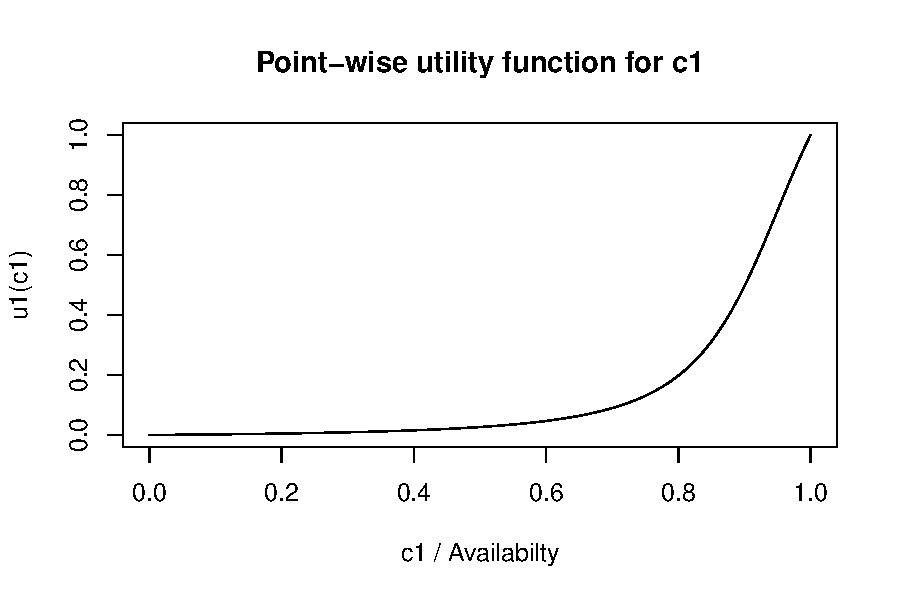
\includegraphics{fig-ds/u1-c1.pdf}
 \caption{Plot of the fitted utility function for point-wise availability; $\tilde{u}_1(c_1)$.\label{Fig:u1-c1}}
\end{figure}
\subsubsection{Utility of warehouse size}
We assume that the smallest warehouse possible is preferred, as this will likely be cheaper. The sizes of the warehouses are $\{50, 75, 100\}$, thus we need $u_2(100) = 0$ and $u_2(50) = 1$. Since the warehouses are discrete decisions, and there are only three warehouses in our problem, it may be better to simply elicit a value for $u_2(75)$ than specify a utility function. However, this would not allow for feedback or analysis of risk aversion. We propose using a risk averse utility function for this part of the problem. A simple, risk averse, form is
\begin{equation}
 u_2(c_2) = 1 - \left(\frac{c_2 - a}{b - a}\right)^2
\end{equation}
where $(a, b)$ are constants to ensure $u(50) = 1$ and $u(100) = 0$. For this problem we have $a = 50$ and $b = 100$. We could then ask the DM what their utility for $c_2 = 75$ is and compare to the value $u_2(75) = 0.75$. We could also try other functional forms. However, since this is an extended illustrative example, we settle on
\begin{equation}
 u_2(c_2) = 1 - \left(\frac{c_2 - 50}{50}\right)^2
\end{equation}
as it reflects realistic beliefs about the problem whilst retaining simplicity.
\subsubsection{Utility of spares restoration}
When spares are restored, we aim to fill up the initial allocation of spares for that particular type of component. We adopt a policy that reflects that spares should be restored as late as possible, without adversely affecting availability. Our utility function should then reflect that restoring the numbers of spares happens as late as possible. Let the number of remaining spare parts for subassembly $i$ be $s_i (t)$ (which from hereon in will be implicitly a function of time). One way to specify when spares are restored is to specify a value $s'_i$ for the $i$th subassembly such that, at the instant when $s_i < s'_i$ is first satisfied, an order for more spare parts is placed. We would like to avoid having a utility function which depends on another decision, since $s'_i \leq s_i$. We can instead express this decision as an independent attribute by finding the proportion of spares, $p_i$ such that when $\frac{s_i}{s'_i} < p_i$ more spares must be ordered, where $p_i \in (1, 99)\%$ is the `critical percentage' for ordering more spares. This phrasing of the problem in terms of proportions has two advantages. It makes specifying the utility function easier, as the proportion and the number of spares are independent attributes. Additionally, maximising $U(\bx)$ when there is a complex dependence structure between elements of $\bx$ will be difficult.

Therefore, the third set of decision variables will be $x_{10:18} = (p_1, p_2, \ldots, p_9)$. The following utility function is an appropriate choice for the restoration policy for the $j$th spare component
\begin{equation}
 u_{3,j}(c_{3,j}) = 1 - \left(\frac{1 - c_{3, j}}{99 - 1}\right)^2
\end{equation}
which is a risk-averse utility function which decreases as $c_{3, j} = x_{j+9}$ increases. To combine this into an overall utility function for the spares restoration policy, we could construct a weighted average
\begin{equation}
 u_3 (c_3) = \sum_{j = 1}^9 k_j u_{3,j}(c_3).
\end{equation}
To elicit the weights, $k_j$, we can apply standard multi-attribute elicitation techniques, such as those in \citet{Gonzalez2018}. We however have no preference for one type of spare over another, hence we take $k_j = \frac{1}{9}$ for all $j$. This results in the utility function for $c_3$ being
\begin{equation}
 u_3(c_3) = 1 - \frac{1}{9}\sum_{j=1}^9 \left(\frac{1 - c_{3, j}}{98}\right)^2.
\end{equation}
\subsubsection{Combining all attributes}
To combine the attributes we will use a probability equivalence
 approach \citep{Gonzalez2018}. Recall that $c^{*}$ is the vector of the best possible set of consequences (those which maximise the marginal utility functions). Also recall that $c^{0}$ is the vector of the worst possible consequences, so, minimum availability, restoring spares as soon as one spare part has been used and opting for the largest warehouse. Recall that $u(c^{*}) = 1$ and $u(c^0)= 0$. Now let $c^{0}_{j}$ be the consequence which has all consequences at their worst value, except the $j$th consequence which takes its best value. We can also extend $j$ to be a collection of consequences (so everything contained in the set $j$ is at its best consequence). We propose using an additive utility function
\begin{equation}
 u(c) = \sum_{j=1}^3 w_j u_j(c_j)
\end{equation}
where $w_j$ are non-negative weights which sum to $1$.

To specify the weights, we elicit $p_1$ such that $[c^{0}, c^{*}; p_1] \sim c^{*}_{j}$. In our case, we settled on the value $p_1 = 0.2$, thus $w_1 = 0.8$. We next elicit $p_2$ such that $[c^{0}, c^{*}; p_2] \sim c^{*}_{(1,2)}$. In this case, we choose $p_2 = 0.1$, hence $w_2 = 0.1$. The sum to unity constraint implies $w_3 = 0.1$. We could ask a feedback question to verify that the weights are reasonable, but we stop here for simplicity. Therefore our final expected utility function, as a function of $\bx$, is
\begin{equation}
 U(\bx) =  0.8U_1(\bx) + 0.1 U_2(\bx) + 0.1 U_3(\bx)
\end{equation}
where $U_i(\bx) = \E_{\btheta}\{u_i(c(\bx, \btheta))\}$ is the expected utility function for the $i$th decision and averaging is performed over all possible consequences induced by decision $\bx$ when the state of knowledge is quantified by $\btheta \sim \pi(\btheta)$.
\section{Decision support strategy}
Our problem is to maximise $U(\bx)$. This is challenging for multiple reasons:
\begin{itemize}
 \item[(1)] $U(\bx)$ is expensive, stochastic and black-box in nature.
 \item[(2)] We want to communicate uncertainty in the solution to the problem, that is, construct a set of `sensible' decisions.
 \item[(3)] $\bx$ has a complex form:
 \begin{itemize}
  \item[(i)] The warehouse aspect of $\bx$ means $U(\bx)$ is a combination of $3$ different, possibly related, functions.
  \item[(ii)] \correction{Since $x_{1:9} \in \mathcal{S}^{8}_n \subset \N^{9}$, with $n \in \N$, the use of gradient-based optimisers is difficult.}
 \end{itemize}
\end{itemize}
To overcome challenges (1) and (2) we will use a hybrid, novel union of BayesOpt and HM inspired techniques. Our approach will be to first perform a run of BayesOpt to find the (approximate) optimal decision, $\hat{\bx}$, then subsequently use rounds of iterative refocussing to rule out clearly sub-optimal decisions. For the refocussing, we will use implausibility measures of the form:
\begin{equation}
 I(\bx) = \frac{\E\{ U(\hat{\bx}) \} - \E\{ U(\bx) \}}{\sqrt{\var \{U(\hat{\bx}) - U(\bx) \}}} \label{Eq:base-implaus}
\end{equation}
where $\hat{\bx} = \argmax_{\bx \in X} m^{*}(\bx)$ where $X$ is the set of inputs at which $U(\bx)$ has been evaluated, and $m^{*}(\bx)$ is given by \cref{Eq:MV1}. That is, the largest expected value of $U(\bx)$. First note that $I(\bx)$ can be negative. $I(\bx) < 0$ indicates that $\bx$ is predicted to be a better decision than $\hat{\bx}$. The next novel feature is that, the denominator of \cref{Eq:base-implaus}, when expanded, will contain a covariance term since $\var\{X - Y\} = \var\{X\} + \var\{Y\} - 2 \cov \{X, Y\}$. The covariance term will vanish if $\bx$ and $\hat{\bx}$ correspond to different warehouses. This choice of implausibility measure is a consequence of our novel approach. It is much more common to assume independence between the `reference' value (data) and the model, since data will typically be generated by a physical process which would be independent of any models. In the case of optimisation, the reference value may have come directly from the simulator, rather than the emulator, as in \citet{Owen2020}, thus we can assume independence. Alternatively, we may have some knowledge of what the maximiser already is, as in \citet{Nguyen2020}. We however will be comparing one emulator prediction to many others and so correlation is present and must be accounted for. We will use a cut off rule $I(\bx) > 3$, motivated by Pukelsheim's $3\sigma$ rule \citep{Pukelsheim1994}, to rule out decisions which are thought to be worse that $\hat{\bx}$.

We approach (3i) by performing separate BayesOpt routines/constructing independent emulators for each warehouse. It may be possible to specify a suitable covariance structure between warehouses, however our approach has some advantages. The first is simplicity; constructing independent emulators is computationally, programmatically and conceptually simpler than a joint emulator for all warehouses. The fact that the choice of warehouse changes the permitted values of $\bx$ could make construction of a joint emulator very challenging. Our approach allows us to make use of large, parallel computing facilities in a simple way. We will perform a BayesOpt run for each warehouse independently of the other warehouses. Using the Rocket HPC facility at Newcastle University allows us to perform the runs for separate warehouses simultaneously. This approach also offers more computationally efficient emulators. When, for each warehouse, we have observed simulator runs at $n$ locations, independent emulator prediction will have cost $\mathcal{O}(n^2)$ and the cost of inference will be $\mathcal{O}(3n^3)$. Note that the cost of prediction is \textit{not} multiplied by $3$ since the inputs tell us which emulator to use for prediction. Joint emulation will have prediction cost $\mathcal{O}((3n)^2)$ and inference cost $\mathcal{O}((3n)^3)$. If another problem requires more warehouses (or in a more general problem, the function to be emulated is composed of more cases), the cost of the joint case will be much greater. If iterative refocussing allows us to rule out a warehouse, then the independent emulation strategy allows us to act as if that warehouse was never part of the problem, providing further computational savings.

Now, (3ii) is dealt with by first relaxing the maximisation of the acquisition function to be over a continuous domain. Let the relaxed maximiser be $\tilde{\bx}$. This may give us an invalid point at which to next run the model (the numbers of spares \textit{must} be integers). To satisfy the integer constraint, we try all valid solutions within a given domain of $\tilde{\bx}$. We construct a set of candidate solutions by rounding each element of $\tilde{\bx}_{1:9}$ either up to the nearest integer or down to the nearest integer. This returns $2^9 = 512$ candidate solutions, not all of which are \textit{valid} candidate solutions. Candidate solutions which do not satisfy $\sum_{i = 1}^9 x_i = x_{19}$ are discarded as they are not members of the decision space. We then evaluate the acquisition function at each of the remaining candidate inputs and then run the simulator at the input from the set of candidate decisions which returns the largest value of the acquisition function. This may not be the true maximiser of the acquisition function, but should be a `good' location at which to query $U(\bx)$.

Note that the iterative refocussing cannot continue \textit{ad infinitum}. We must terminate the procedure at some point. When any of the following conditions hold, we should stop the procedure \citep{Vernon2010}:
\begin{itemize}
 \item[(1)] Emulator variance is much smaller than other sources of uncertainty.
 \item[(2)] Computational resources have been exhausted.
 \item[(3)] The entire parameter space has been ruled out as implausible.
 \item[(4)] The reduction in the size of the NROY volume is negligible.
\end{itemize}
Note that in our analysis, condition (3) will never happen as the maximum value cannot be ruled out. In our analysis, we will not consider other sources of uncertainty such as model discrepancy, but they can be incorporated and used to terminate HM. See \citet{Ling2014} and \citet{Brynjarsdottir2014} for guidance on eliciting model discrepancy. Our stopping mechanism will be exhausting our computational resources and/or observing a negligible change in the NROY region.

We have described all relevant details of our problem and motivated appropriate methodology for decision support. A succinct description of our approach is as follows:
\begin{itemize}
 \item[1.] Run the simulator at collection of inputs to construct a Wave $1$ emulator. We will use BayesOpt to choose the design points.
 \item[2.] Find the (approximately) optimal decision $\hat{\bx}$ and run a HM procedure to construct the NROY set.
 \item[3.] Within the NROY set, construct a space-filling design and run the simulator at these design points.
 \item[4.] Fit an emulator to the new training data and run a HM procedure to construct the new NROY set.
 \item[5.] If none of the stopping criteria are met, go to step 2. Otherwise, terminate the procedure and report the NROY set to the DM.
\end{itemize}

\section{Wave $1$: Bayesian optimisation}
\subsection{Volume of the initial decision space}
Prior to performing any intensive calculations we will first calculate the volume of the non-implausible region. Typically this would be $1$ as, usually, all inputs are continuous and can be rescaled to occupy $[0,1]^p$ for some $p \in \N$. In our problem, we have discrete inputs. We assign each warehouse-spares combination a volume of $1$. This is the volume implied by the spares restoration policy. Now the initial decision space, $\calX_1$, is given as
\begin{equation}
 \calX_1 = \bigcup_{n \in \{50, 75, 100\}} (\mathcal{S}^8_{n} \times (1, 99)^9).
\end{equation}
Now we will count the numbers of ways to fill each warehouse with spares. For warehouse $i$ let this number be $V_i$. The total volume is $|\calX_1| = V = \sum_{i=1}^3 V_i$. The number of members of $\mathcal{S}^k_n$ is ${n-1 \choose k}$. This is because, using the `standard' definition of the discrete simplex, denoted $\mathcal{T}^k_t$ where $x_i \in \{0, 1, \ldots, t\}$ and $\sum_{i=1}^{k+1} x_i = t$ has size $|\mathcal{T}^k_t| = {t+k-1 \choose k}$ \citep{Costello1971}. Substituting $t = n-k$ gives $|\mathcal{S}^k_n| = {n-1 \choose k}$.

Now, if each discrete decision has volume $1$, then the total volume of the decision space is
\begin{align*}
 V &= {49 \choose 8} + {74 \choose 8} + {99 \choose 8}\\
 &= 450978066 + 15071474661 + 171200862756\\
 &= 186723315483 \approx 2 \times 10^{11}
\end{align*}
which is also the number of spares-warehouse combinations.

\subsection{BayesOpt implementation details}

The first emulator will be a homoscedastic Gaussian process emulator constructed by employing BayesOpt techniques. As noted before, emulators for different warehouses are independent of each other. The remaining decision variables, $x_1$ -- $x_{18}$ can then be fed into the emulator. These variables are transformed to a $[0,1]$ scale. From hereon, when we refer to (elements of) $\bx$, we will mean the version scaled to $[0,1]$, unless stated otherwise. Now since the first $9$ inputs sit on a simplex, one of them is redundant, given the rest. Therefore, our emulators only use the decision variables $x_2$ -- $x_{18}$. We can also show that inclusion of $x_1$ alongside $x_2$ -- $x_9$ induces a non-stationary covariance function. This is because $(x_1 - x_1')^2 = \left[ (1 - \sum_{i=2}^9 x_i) - (1 - \sum_{i=2}^9 x'_i) \right]^2$. This may also cause identifiability issues with any lengthscale parameters, as the distance between individual elements of $\bx$ and $\bx'$ essentially appears twice.

In the BayesOpt stage, we use a simple constant-mean GP with all parameters estimated via a MAP estimate. Recall we are trying to optimise $U(\bx)$, which depends on the expensive, stochastic Athena simulator. Since we view our approach as a unification of decision making and decision support, we will use an acquisition function that can be employed in the Bayes linear or fully Bayesian frameworks. Our acquisition function will be a UCB acquisition function with $\nu_n = 3$:
\begin{equation}
 \alpha_n(\bx) = \mu_n(\bx) + 3 \sigma_n(\bx).
\end{equation}
We have chosen $\nu_n = 3$ to tie in with the future rounds of iterative refocussing --- this choice of acquisition function is related to many common implausibility measures. Thus, if $U(\bx) = \mu_n(\bx) + 3 \sigma_n(\bx)$ it would have small implausibility. The choice of $\nu_n = 3$ is a fairly large value for $\nu_n$; we are encouraging more exploration. One argument against using a GP in this example is that the utility function is constrained to $(0,1)$ but the GP predictions occupy the full real line. We are simply using the GP as a computationally convenient modelling choice. Note that in earlier stages of the BayesOpt routine, it is likely that for some values of $\bx$ that $\mu_n(\bx) + 3 \sigma_n(\bx) > 1$. This will be because $\sigma_n(\bx)$ is large. However if $\mu_n(\bx) + 3 \sigma_n(\bx) > 1$ it is likely that we will be query $U(\cdot)$ at a point close to $\bx$ and the uncertainty will be resolved. Therefore, by the end of the BayesOpt routine, predictions should lie in $(0,1)$ with high probability.

We run a BayesOpt scheme for each of the three warehouses. The idea is to find the best possible inputs for each warehouse to give it the best possible chance of being retained as NROY. The data in this instance will be realisations of $u(\bx)$, with individual realisations denoted by $u(\bx)_i$. To fit and train emulators, a single `observation' will be the mean of $30$ i.i.d. realisations of $u(\bx)$, that is
\begin{align}
 y(\bx) &= \frac{1}{30} \sum_{i = 1}^{30} u(\bx)_i\\
   & = U(\bx) + \varepsilon
\end{align}
where $\varepsilon \iid \mathcal{N}(0, \lambda^2)$ is assumed random error. The choice of $30$ replicates is a trade-off between computing time and accuracy. A small number of replicates will be inexpensive, but give a noisy perspective of $U(\bx)$. A larger number of replicates will give a clearer perspective of $U(\bx)$, and, by the Central limit theorem (CLT), a large enough number of replicates means $y(\bx)$ should be approximately Normal.

Each scheme will be initialised with $40$ $(\bx, y)$, pairs with the initial design chosen by simple random sampling. The GP hyperparameters are estimated based on these $40$ runs. Since this is a small sample size, we update the GP hyperparameters after every $40$ acquisitions. We perform acquisitions until we have observed $1000$ $y$ values, or the pre-defined wall-clock simulation time has elapsed. Usually, BayesOpt terminates when an optimisation-based stopping rule is satisfied. However, since $U(\bx)$ is not observed perfectly, but with noise, there will be uncertainty about $U(\bx)$ for finite numbers of replications and observations. Performing additional acquisitions \textit{after} conventional stopping rules have been satisfied, allows us to reduce uncertainty about $U(\cdot)$. This allows us to reduce uncertainty about the optimal decision $U(\hat{\bx})$ which, in turn, may lead to smaller NROY spaces after iterative refocussing or HM. This should further simplify the decision that the DM has to make, as the final NROY volume should be smaller than if we terminated BayesOpt when a stopping rule has been met.
\subsection{Wave $1$ results \& analysis}
Once the BayesOpt schemes had been run, we checked the quality of the fitted emulators via a leave-one-out (LOO) procedure. We used a standard LOO procedure; re-fitting the emulators without $(\bx_i, y_i)$ and then use this reduced data set to predict $y_i$. Let the LOO prediction for $y_i$ have mean $m_i$ and variance $v_i$. We then define standardised LOO prediction errors by $\text{SLPE}_i = (y_i - m_i)/\sqrt{v_i}$. These showed, that for each warehouse, there was an issue with $x_9$. The plots within \cref{Fig:first-loo} show a `tail' of residuals for small values of $x_9$ (the catch all subassembly). For larger values of $x_9$, the cloud of residuals looks uncorrelated. Plots of SLPEs against each input (for every warehouse) are given in \cref{App:resid1}.
\begin{figure}
 \centering
 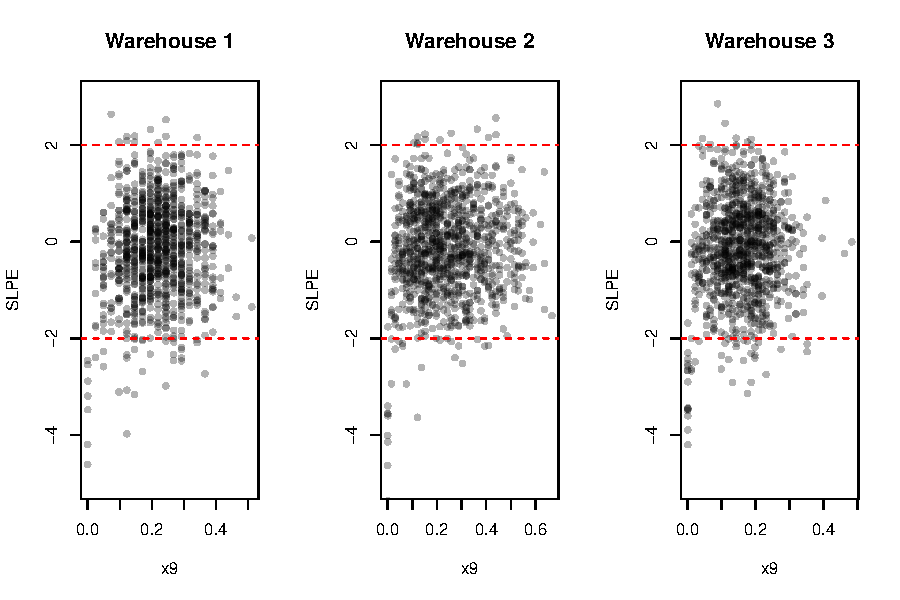
\includegraphics{fig-ds/first-resids.pdf}
 \caption{SLPEs plotted against $x_9$; the dashed red lines denote $\pm 2$ and the $x$ axis is on the standardised $[0,1]$ scale. We see, in each case, that there is a `tail' of residuals for small values of $x_9$. Each emulator has at least one SLPE larger than $4$ in modulus, suggesting a serious discrepancy between the emulator and $U(\bx)$. The vertical bands of residuals are present since $x_9$ takes values from a finite set. \label{Fig:first-loo}}
\end{figure}
To improve the emulator, we introduced a non-constant mean function: $\mu(\bx) = \beta_0 + \beta_1 \log (x_9 + 10^{-8})$. The addition of $10^{-8}$ avoids the undefined value $\log(0)$. The value $10^{-8}$ could be replaced by an unknown constant to be inferred, but we found that this initial guess value to satisfactory emulators. For the revised emulators, we integrated out the $\beta$ coefficients by adopting the prior specification $\beta_i \iid \mathcal{N}(0, 0.5^2)$ for $i \in \{0, 1\}$. This led to emulators with improved LOO diagnostics, which are illustrated in \cref{Fig:second-loo}. These residuals suggest that the revised emulator offers a better estimate of $U(\bx)$ than the first emulator. In this section we have only shown the SLPEs plotted against $x_9$; plots of SLPEs against inputs $x_1$ -- $x_{18}$ are given in \cref{App:resid2}.
\begin{figure}
 \centering
 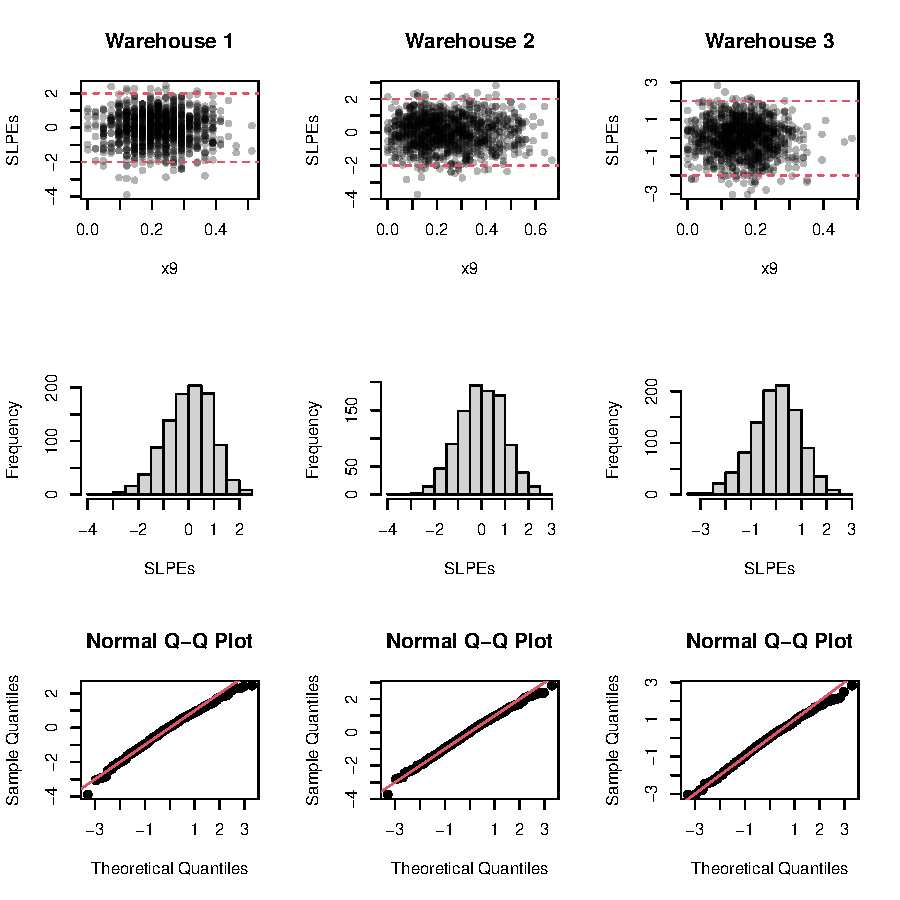
\includegraphics{fig-ds/second-resids.pdf}
 \caption{A suite of diagnostics based on SLPEs, organised in columns. Left column corresponds to Warehouse $1$, the middle column to Warehouse $2$ and the right column to Warehouse $3$. The top three plots show the SLPEs plotted against $x_9$ after incorporating the prior mean function $\mu(\bx) = \beta_0 + \beta_1 \log (x_9 + 10^{-8})$. Dashed red lines are at $\pm2$. The second row of plots are histograms of the SLPEs and the final row are Normal QQ plots, where the red line is the unit diagonal.\label{Fig:second-loo}}
\end{figure}
 A suite of diagnostic plots in \cref{Fig:second-loo} suggest that the emulator is an improved and appropriate surrogate for $U(\bx)$; the LOO residuals now appear to be uncorrelated with $x_9$, the histograms of the LOO errors are close to that of a standard Normal distribution (the distribution of SLPEs for Warehouse $1$ has a slightly longer left tail than one might expect) and the QQ plots further indicate the LOO errors are well described by a standard Normal distribution. We also verify that the cut off of $3$ is appropriate by checking quantiles of the Normal distribution. \cref{Tab:cred1} shows that over $95\%$ of the LOO errors lie in $(-3,3)$, thus there is agreement with Pukelsheim's $3\sigma$ rule and we are now in a position to rule out inappropriate decisions.
\begin{table}
 \centering
 \begin{tabular}{rrrr}
  \toprule
  Warehouse & SLPE Interval & Expected Proportion & Observed Proportion \\\cmidrule{1-4}
  $1$ & $(-2,2)$&$0.95$ & $0.968$\\
  &$(-3,3)$& $0.997$ & $0.998$ \\\cmidrule{1-4}
  $2$ & $(-2,2)$&$0.95$ & $0.967$\\
  &$(-3,3)$& $0.997$ & $0.999$ \\\cmidrule{1-4}
  $3$ &$(-2,2)$& $0.95$ & $0.964$\\
  &$(-3,3)$& $0.997$ & $0.998$ \\\bottomrule
 \end{tabular}
 \caption{Comparing the expected proportion to the observed proportion of SLPEs to lie within given intervals, assuming Normality of the SLPEs. The observed proportions are those from the improved emulator.}
 \label{Tab:cred1}
\end{table}
\subsection{Ruling out decisions}
Using the improved emulator, we can find the design point, $\hat{\bx}$, which maximises $\E\{U(\bx)\}$. In this case, $\hat{x}_{19} = 50$, so the decision belongs to Warehouse $1$. The other elements of $\hat{\bx}$ are given in \cref{Tab:optimiser}. Our uncertainty about $U(\hat{\bx})$ is characterised by
\begin{equation}
 U(\hat{\bx}) \sim \mathcal{N} (0.8314, 8.749 \times 10^{-5})
\end{equation}
\begin{table}
 \centering
 \begin{tabular}{lrrrrrrrrr}
  \toprule
  $i$ &1&2&3&4&5&6&7&8&9\\\cmidrule{1-10}
  $\hat{x}_i$& 1 & 4 & 9 & 7 & 2 & 4 & 9 & 1 & 13\\
  $\hat{x}_{i+9}$ &57.03 & 39.96 & 42.07 & 28.25 & 2.29 & 40.25 & 46.62 & 1.32 & 57.5\\
  \bottomrule
 \end{tabular}
 \caption{The estimated optimal decision reported on the decision scale rather than the $[0,1]$ scale. The warehouse is absent from the table and this decision corresponds to Warehouse $1$. The top row of variables corresponds to the number of spares of type $i$, the bottom row corresponds to the critical percentage for spares of type $i$. \label{Tab:optimiser}}
\end{table}
Now, Warehouse $1$ is in the NROY space as $I(\hat{\bx}) = 0$. We constructed a random, uniform sample of decisions ($N = 10^5$) within each warehouse and found that $90.87\%$ of decisions corresponding to Warehouse $1$ satisfied $I(\bx) < 3$ ($95\%$ CI: $(90.81, 90.93)\%$) whereas only $1.4 \times 10^{-3}\%$ of decisions corresponding to Warehouse $2$ are NROY ($95\%$ CI: $(6.52, 21.5)\times 10^{-3}\%$). Credible intervals were found using a Binomial model for the number of observed NROY decisions within Warehouse $i$, $M_i$, from a sample of $N_i$ random and uniformly distributed decisions. If the proportion of NROY decisions is $\alpha_i$ then \textit{a priori} $\alpha_i \sim Beta(a_i, b_i)$ and the sampling model for the number of NROY decisions observed from a random sample is $M_i \mid \alpha_i \sim Binomial(N_i = 10^5, \alpha_i)$. It is well known that the distribution of $\alpha_i \mid M_i$ is given by
\begin{align}
 \alpha_i \mid M_i &\sim Beta(A_i, B_i) \\
 A_i & = a_i + \sum_{j=1}^{N_i} \mathbb{I} ( I(\bx_{i,j}) \geq 3)\\
 B_i & = b_i + \sum_{j=1}^{N_i} \mathbb{I} ( I(\bx_{i,j} ) < 3)
\end{align}
where $\bx_{i,j}$ is the $j$th candidate decision for Warehouse $i$. For each warehouse, we took a flat prior for $\alpha$ ($a_i = b_i = 1$) and then the credible intervals are found as the $95\%$ highest posterior density intervals for $\alpha_i \mid M_i$.

Our random sample returned $0$ decisions in Warehouse $3$ that were NROY. To see if we could conclusively rule out Warehouse $3$ as a sub-optimal decision, we minimised the implausibility function for Warehouse $3$. To simplify the minimisation, we treated the discrete inputs as continuous. After running the optimiser $20$ times, our minimum implausibility was $\min I(\bx) = 7.36 > 3$. We are therefore satisfied that all decisions corresponding to Warehouse $3$ will be ruled out.

The nature of the NROY space for Warehouse $1$ is shown in \cref{Fig:wave1-w1-nroy}. We see that most decisions are green (NROY). The red, ruled-out decisions all seem to be those with very small values of $x_9$. For warehouse $2$, only $14$ out of $10^6$ points from the large random sample were retained as NROY. We have therefore presented only the NROY samples in \cref{Fig:wave1-w2-nroy}. For Warehouse $2$ we see that every $x_{10:18} < 0.5$ on the $(0,1)$ scale. This suggests a larger warehouse size affords us more time to buy in spares.
\begin{figure}
  \centering
  \includegraphics[width = 8in, angle=270]{fig-ds/wave1-wh1-landscape.pdf}
  \caption{A large uniform sample of decisions corresponding to Warehouse $1$. Green decisions are those that are NROY and red have been ruled out. Although $x_1$ was not explicitly included in the emulator, we have included it in this figure. Further note that the first $9$ inputs have been jittered with $\mathcal{N}(0, 9 \times 10^{-6})$ noise to aid visualisation. \label{Fig:wave1-w1-nroy}}
\end{figure}
\begin{figure}
  \centering
  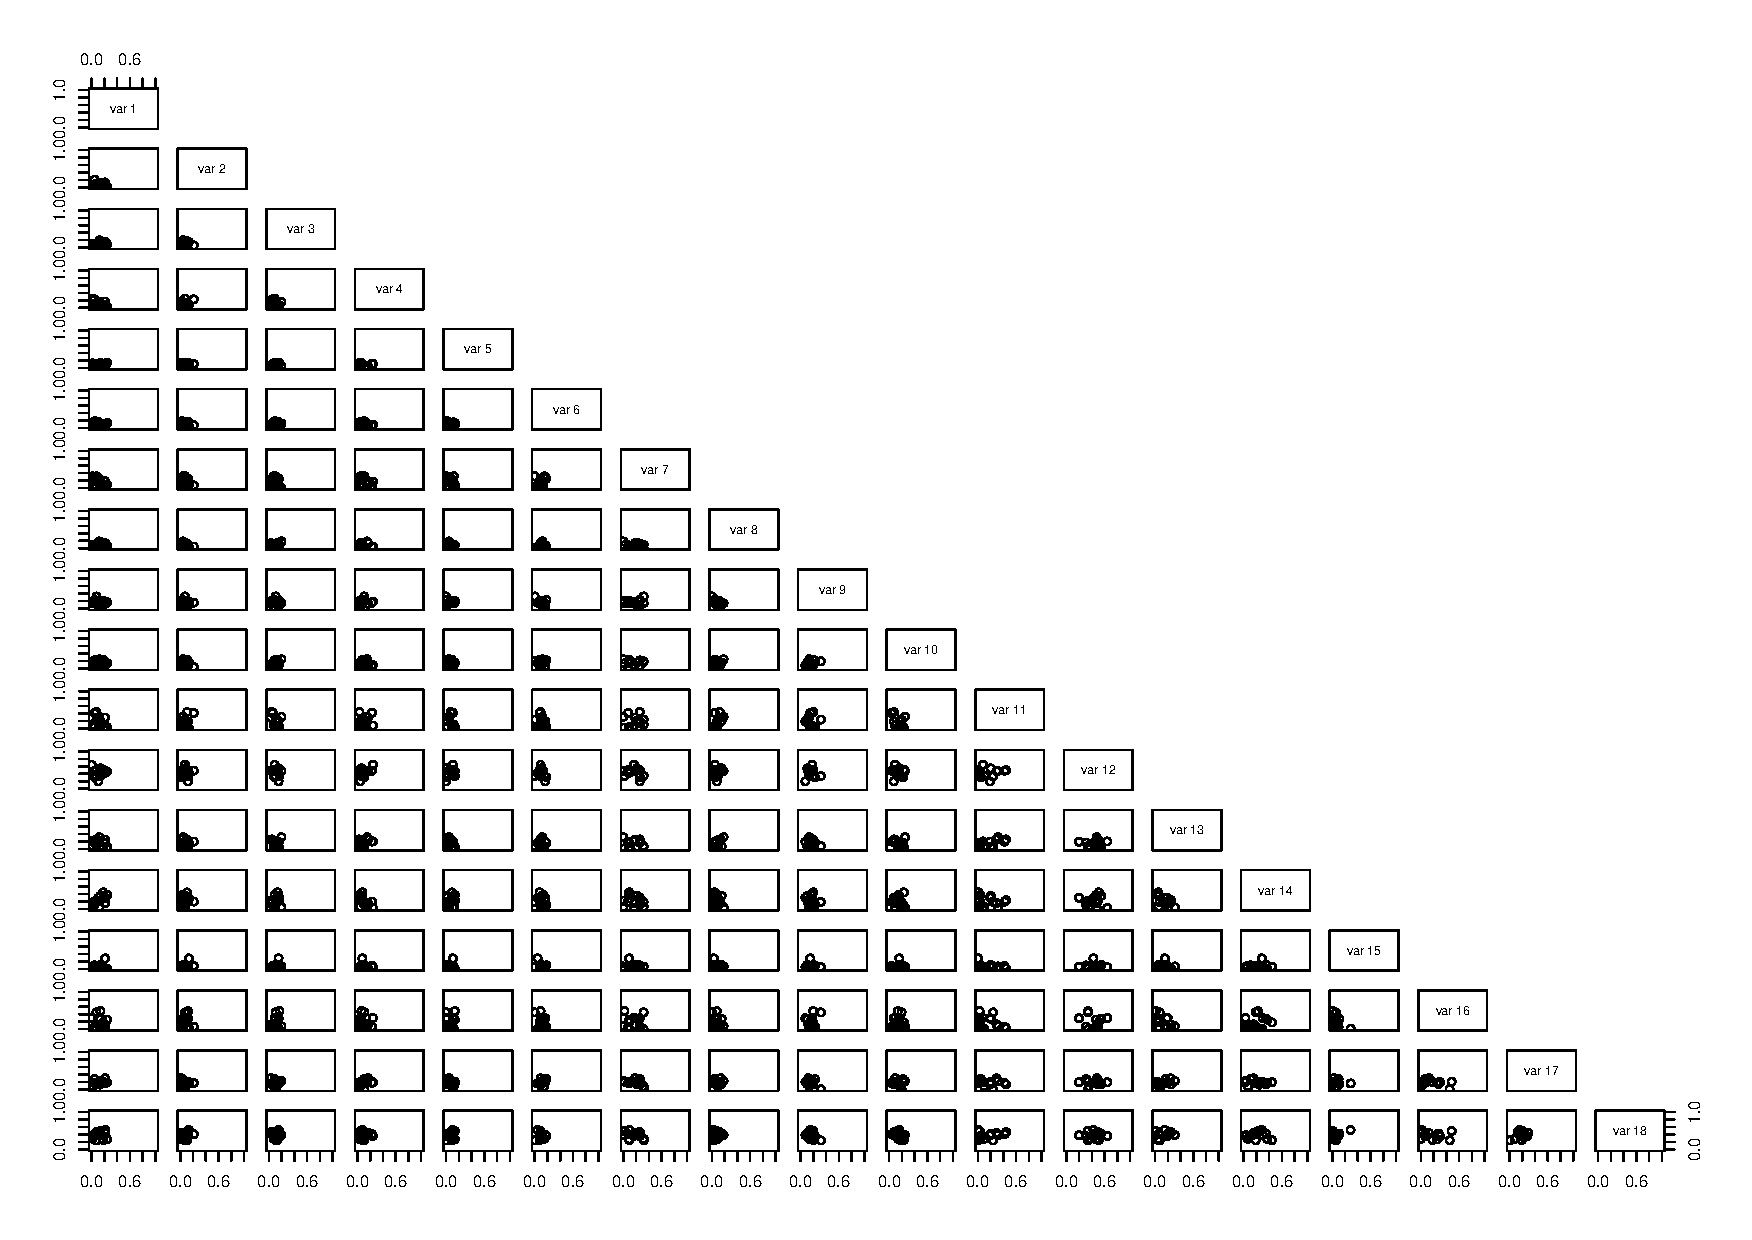
\includegraphics[width = 8in, angle=270]{fig-ds/wave1-wh2-landscape.pdf}
  \caption{A collection of NROY decisions corresponding to Warehouse $2$. Although $x_1$ was not explicitly included in the emulator, we have included it in this figure.\label{Fig:wave1-w2-nroy}}
\end{figure}

We have greatly simplified the analysis for the DM by applying a post-hoc history matching inspired idea to the BayesOpt routine to find decisions which are consistent with the approximate maximiser and find those which are clearly suboptimal. If desired, this would be a sensible place to stop the analysis and report our findings to the DM. However, the HM literature has shown that further probing can be advantageous \citep{Jackson2018, Vernon2022}.

\subsection{Constructing a wave $2$ design}

We follow the convention of further investigation within the NROY space to refine the set of sensible decisions. To do so, we need a design for a wave $2$ emulator. For Warehouse $1$, since the remaining NROY volume is quite large, simple rejection sampling will lead to a uniform design without much trouble. For Warehouse $2$, the NROY volume is a small fraction of the original volume, consequently, rejection sampling is inefficient.

To overcome the inefficiency of rejection sampling, we employ an adapted version of the slice sampler presented by \citet{Andrianakis2017a}. The adaptation addresses the discrete simplex aspect of the decision space and is presented in \cref{Alg:disc-slice}. The sum to unity constraint on the simplex means one decision variable is determined, given the rest. This algorithm does not include any continuous-valued components of $\bx$, however, since the algorithm is component-wise, we can first update the set of discrete components and then update the set of continuous components using \cref{alg:nroy-slice}.

\begin{algorithm}[h]
\caption{A single sweep of a component-wise slice sampler for generating NROY samples within the discrete simplex. \label{Alg:disc-slice}}
\begin{algorithmic}
\Require An indicator function $\mathbb{I}(\bx \in \calX_{k+1})$ for identifying inputs which are NROY, an initial NROY point $\bx_0 \in \calX_{k+1}$ where $\bx_0$ is an $m$ dimensional parameter vector. A set of $q+1$ unique, equally spaced, values $\mathcal{S} = \{ d_0, d_1, d_2, \ldots, d_{q-1}, d_q \}$ where $0 = d_0 < d_1 < \ldots < d_{q-1} < d_q = 1$.
\State $\bx^{*} \gets \bx_0$
\For{$i = 1$, $2$, $\ldots$, $m$}
 \State $I^{*} \gets 0$ \Comment{Initialise an indicator variable}
 \While{$I^* \neq 1$}
  \State Compute $d_p = 1 - \sum_{j \neq i} x^{*}_j$
  \State Draw $x_i \sim \mathcal{U} \{ d_0, d_1, d_2, \ldots, d_p \}$ \Comment{Change the $i$th input}
  \State $x^{*}_i \gets x_i$
  \State $x^{*}_1 \gets 1 - \sum_{j = 2}^m x_j^{*}$ \Comment{Force sum to unity constraint}
  \State $I^{*} \gets \mathbb{I}(\bx^{*} \in \calX_{k+1})$ \Comment{Evaluate the implausibility measure at the new input}
 \EndWhile
\EndFor
\State $\bx_1 \gets \bx^{*}$
\State Return $\bx_1$, the new NROY sample.
\end{algorithmic}
\end{algorithm}
\correction{As with \cref{alg:nroy-slice}, \cref{Alg:disc-slice} is not ergodic. However, as with \cref{alg:nroy-slice}, we can adapt \cref{Alg:disc-slice} to become ergodic in a similar way to \cref{alg:ergodic-slice}: we essentially re-run the algorithm from a collection of randomly chosen starting points. We write this out explicitly in \cref{alg:ergodic-disc-slice}.}

\begin{algorithm}[h]
\caption{An ergodic algorithm for simulating uniformly on of $\mathcal{S}^n_q \times [0, 1]^p$. \label{alg:ergodic-disc-slice}}
\begin{algorithmic}
\Require An indicator function $\mathbb{I}(\bx \in \calX_{k+1})$, a set of $q+1$ unique, equally spaced, values $\mathcal{S} = \{ d_0, d_1, d_2, \ldots, d_{q-1}, d_q \}$ where $0 = d_0 < d_1 < \ldots < d_{q-1} < d_q = 1$, the number of continuous inputs, $p$,  a number of replications, $R$, a required number of samples, $n =  n' \times R$, and a function $\texttt{slice\_sampler\_one\_step}(\mathbb{I}(\bx \in \calX_{k+1}), \bx_0)$ which takes an NROY point $ \bx_0 \in \calX_{k+1} \subseteq \mathcal{S}_q^n \times [0, 1]^p$, and returns a new NROY point.
\For{$r = 1, 2, \ldots, R$}
  \State {$I_r \gets 0$}
  \State Initialise a matrix $X_r$ with $m$ columns and $n'$ rows
  \While{$I_r \neq 1$}
    \State $\bx_{1, r} \gets \mathcal{U}(\mathcal{S}_q^n \times [0, 1]^p)$ \Comment{Simulate uniformly from the cross product of $\mathcal{S}^n_q$ and $[0, 1]^p$ }
    \State $I_r \gets \mathbb{I}(\bx{1, r} \in \calX_{k+1})$
  \EndWhile
  \For{$i = 2, 3, \ldots, n'$}
  \State $\bx_{i, r} \gets \texttt{slice\_sampler\_one\_step}(\mathbb{I}(\bx \in \calX_{k+1}), \bx_{i-1, r})$
\EndFor
\EndFor
\State Collect all $X_r$ into a single matrix $X$, with $m$ columns and $n$ rows.
\State Return $X$, the collection of uniformly distributed NROY samples.
%\Return $X$, a sample of $n$ NROy points.
\end{algorithmic}
\end{algorithm}

For low-dimensional, continuous-valued simplices, uniform sampling typically gives reasonable coverage of the margins. However, as the dimension increases, we encounter a problem. It becomes increasingly difficult for large values of $x_i$ to be sampled. Although we work with a discrete simplex, a continuous-valued simplex is easier to analyse and provides us with a good intuition for the marginal behaviour of a discrete simplex.

A uniform sample on the $k$ dimensional, continuous simplex is equivalent to sampling from a $Dirichlet(1_{k+1})$ distribution, where $1_{k+1}$ is a length $(k+1)$ vector of $1$s. A well known result states that if $\bm{X} \sim Dirichlet(\bm{\alpha})$ then the marginal distributions are given by $X_i \sim Beta(\alpha_i, \alpha_0 - \alpha_i)$ where $\alpha_0 = \sum_{j=1}^{k+1} \alpha_j$. Applying this result to the simplex means that a uniform sample on the $k$ dimensional simplex has $Beta(1, k)$ margins. Now for any $b \in (0,1)$, $\Pr (X_i > b) \to 0$ as $k \to \infty$. Although we have stated an asymptotic result, the effects are present even for moderate values of $k$. In \cref{Fig:beta-plot} we see plots of $\Pr (X_i > b)$ for various choices of $b$ over the range $k = 1, 2, \ldots, 13$. Note that we have $k = 8$ and thus $\Pr(X_i > 0.2) = 0.17$, $\Pr(X_i > 0.4) = 0.017$, $\Pr(X_i > 0.6) = 6.6 \times 10^{-4}$ and $\Pr(X_i > 0.8) = 2.6 \times 10^{-6}$. With emulators, we often have quite small samples sizes. Typically, designs have at most $1000$ points. From a decision support perspective, this is worrying. We want to consider a diverse set of decisions with a relatively small sample size. Therefore, we aim to construct a design which fills the space or, at least, targets areas of the decision space which are uncertain. This is especially important for Warehouse $1$ as the current NROY space is almost all of the Warehouse $1$ space.
\begin{figure}
 \centering
 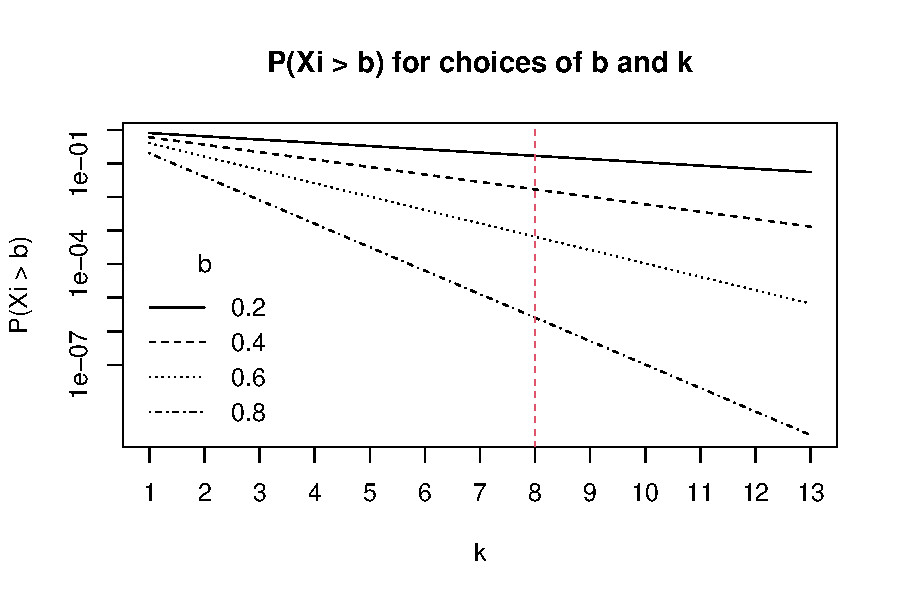
\includegraphics{fig-ds/beta-plot.pdf}
 \caption{Lines showing how $\Pr(X_i > b)$ decreases with $k$, the dimension of the simplex. The vertical, red dashed line corresponds to $k = 8$, the dimension of the simplex in our wind farm example. The black lines of various types correspond to different values of $b$. Note that the $y$ axis is on the logarithmic scale. \label{Fig:beta-plot}}
\end{figure}

One way to alleviate this problem is to force the design points to be far apart. This is a standard procedure. For example, maximin LHs achieve this goal by forcing the closest points to be as far away as possible, that is, maximising the minimum distance between design points. Our approach to `filling the space' will be to construct an approximate ALM (Active Learning McKay, \cref{Eq:std-alm}) design of size $n$. This exploits the fact that, in certain circumstances, posterior GP covariance matrices depend only on the locations of the design points and \textit{not} the response $y = f(\bx)$. The posterior design matrix will usually rely on parameters estimated from the data therefore there is some dependence on $y$. However, we can use estimated parameters from a previous experiment or specify the parameters. For a single warehouse, we proceed in the following way: first construct a large, uniform design within the NROY space of size $N>>n$. Call this design $\tilde{\calX}$. Next, using assumed GP hyperparameters (from the previous wave, for example), find the point $\bx^{(1)} \in \tilde{\calX}$ which maximises $\var\{ U(\bx) \}$. If a constant mean function is used, all points will have equal variance and so a random sample from $\tilde{\calX}$ can initialise the procedure. We then remove $\bx^{(1)}$ from $\tilde{\calX}$ and find the next point with largest variance, call this point $\bx^{(2)}$. We keep repeating this procedure until we have obtained $\bx^{(n)}$. Then the set $X = \{\bx^{(1)}, \bx^{(2)}, \ldots, \bx^{(n)}\}$ will be an approximate ALM design. Increasing $N$ will likely lead to a better approximation to an exact ALM design. Finding $\argmax_{\bx \in \tilde{\calX}} \var \{ U(\bx) \}$ is achieved by computing $\var \{ U(\bx) \}$ for all $\bx \in \tilde{\calX}$. This approach is useful in two ways. Firstly it allows us to construct a space-filling design, but it also allows us to perform post-processing of the slice sampler. Since the slice sampler is an MCMC method, the design is prone to auto-correlation. This post processing via ALM allows us to cope with a potentially autocorrelated MCMC chain. Rather than thinning the chain by a fixed factor (keeping every $t$-th iteration), we automatically choose points which are not close to each other.

We used this approach for both the remaining warehouses. The slice sampler was used to generate $N = 10^5$ candidate points for ALM designs of $n = 10^3$. For an ALM design, we first tried two different approaches. The first approach utilised our knowledge of $U(\bx)$ and used the GP hyperparameters of the emulator with mean function $h(\bx) = \beta_0 + \beta_1 \log (x_9 + 10^{-8})$. Since the emulator was fitted using an empirical Bayes approach, the posterior distribution of each $(\beta_0, \beta_1)$ pair is a direct consequence of the multivariate Normal equations. Therefore, we use the wave $1$ posterior for the $\beta$ parameters as the prior for the wave $2$ emulators. This means that our ALM acquisition function, for warehouse $i$, is
\begin{eqnarray}
 \alpha_i(\bx) = \sigma^{2}_{i} + h(\bx)B_ih(\bx)^T - K_i(\bx, X') \left\{K_i(X', X') + \lambda_i^2\right\}^{-1} K_i(X', \bx) \label{Eq:alm-nroy}
\end{eqnarray}
where $i \in \{1, 2\}$ denotes the choice of warehouse, $K_i(\bx, \bx') = h(\bx) B_i h(\bx)^T + C_i(\bx, \bx')$ is the GP covariance function for warehouse $i$ where $B_i = \var\{\beta^{(i)} \mid \mathcal{D}^{(i)} \}$, $\mathcal{D}^{(i)}$ is the set training data for warehouse $i$. $C_i(\bx, \bx')$ is the covariance function for the residuals from the mean function of warehouse $i$; we assume a squared exponential covariance function. As in \cref{Eq:alm-nroy}, $X'$ represents all locations already in the design. That is, points used to initialise the design as well as those that have been acquired. The second approach relied less on our knowledge of $U(\bx)$. The second design did not use knowledge of the mean function and thus the covariance function was simply a squared exponential. This is achieved by setting $B_i = 0$. We will call the first type of ALM design (with mean) ALMa, and the second (without mean) will be called ALMb. The hyperparameters of each squared exponential covariance function were taken from the wave $1$ emulators.

The ALM post-processing of each MCMC chain took approximately $4.5$ hours. This gave designs which led to $x_i$, for $i \in \{1, 2, \ldots, 9\}$, having wider margins than a random, uniform design of the same size. For this particular problem, the ALMa approach led to margins which were wider than uniform, as did the ALMb design.

The differences between the ALM designs and the uniform design for Warehouse $2$ are more subtle. We suspect this less dramatic difference is due to the fact that the NROY volume within the Warehouse $2$ space is a small subset of the original Warehouse $2$ space. \cref{Fig:alm-vs-unif2} shows that, again, the range of each margin for the ALM designs are typically wider than the uniform design. Some of the uniform margins are wider then the corresponding ALM margins, but those that are wider are only wider by a small amount. In both cases, the difference between the ALMa and uniform design for $x_9$ is very large. This is because we used a non-constant mean function which depends on $x_9$. In particular, the functional form $\beta_0 + \beta_1 \log (x_9 + 10^{-8})$ has large in magnitude values for small $x_9$. Since the variance is essentially the square of this, $\var\{\beta_0 + \beta_1 \log (x_9 + 10^{-8})\}$ is maximised when $x_9 = 0$.
\begin{table}
\centering
\begin{tabular}{rrr}
\toprule
  & \multicolumn{2}{c}{Warehouse} \\\cmidrule{2-3}
Design & $1$ & $2$ \\\cmidrule{1-3}
 ALMb & $0.72$ & $0.17$ \\
 Uniform & $0.35$ & $0.15$ \\\bottomrule
\end{tabular}
\caption{Values of $\min_{\bx, \bx' \in X} \rho (\bx, \bx')$, where $X$ is either the ALMb or the uniform (slice sampling) design. \label{Tab:min-distances}}
\end{table}

This led to the marginal density of $x_9$ having unsatisfactory properties. A comparison of the three designs is given in \cref{Fig:compare-x9}. This figure shows the marginal density of $x_9$ under three design schemes. ALMa, the ALM design which utilised knowledge of the mean function, is clearly not space-filling. For example, $985$ out of the $1000$ points are all exactly the same value, and there is a huge void from $0.2$--$0.8$. The uniform design gives a more diverse set of candidate decisions for us to query, but we see that the largest value of $x_9$ is $0.585$. ALMb provides a wide range of decisions (slightly narrower than ALMa) and lacks holes in the design. Since ALMb has a large range, but does not have any holes, we will use this design for our wave $2$ experiment. Maximising minimum distance is a common design heuristic. We computed the minimum distances, $\min_{\bx, \bx' \in X} \rho (\bx, \bx')$, where $\rho(\cdot, \cdot)$ is Euclidean distance, for the ALMb and uniform designs, which are given in \cref{Tab:min-distances}. We see that the minimum distances for the ALMb designs for warehouses $1$ and $2$ are larger than the minimum distances for the corresponding uniform designs, thus the ALMb designs improves a standard design heuristic. We also want to quantify how much larger, on average, the range of the ALMb design is than the uniform design. An appropriate metric here will the geometric mean of the relative widths of the margins of one design to the other:
\begin{equation}
 \delta_g (i) = \left( \prod_{j=2}^{18} \frac{\delta_{\text{ALMb},i,j}}{\delta_{\text{Uniform},i,j}} \right)^{\frac{1}{17}}
\end{equation}
where $\delta_{D, i, j}$ denotes the range of margin $j$ within warehouse $i$ for design type $D$. Our design has $17$ degrees of freedom and so we have removed the index $j=1$ from the product. Now we have $\delta_g(1) = 1.13$, which indicates, in a multiplicative sense, that the ALMb design has margins which are, on average $13\%$ wider than uniform. We also have $\delta_g(2) = 1.14$, so again, the ALMb design offers an improvement.

A similar effect is seen for $x_9$ within warehouse $2$. We see (\cref{Fig:compare-x9-2}) that, to a lesser extent than warehouse $1$, that the ALMa design has a large clump of points at the lower end of the range. The uniform and ALMb designs appear to be similar (apart from a small shift in location), perhaps this is because the NROY volume for warehouse $2$ is a fairly small fraction of the original space and thus, many extreme values may have been ruled out. Since we will be using the ALMb design, from hereon in we will refer to it as the ALM design.
\begin{figure}
 \centering
 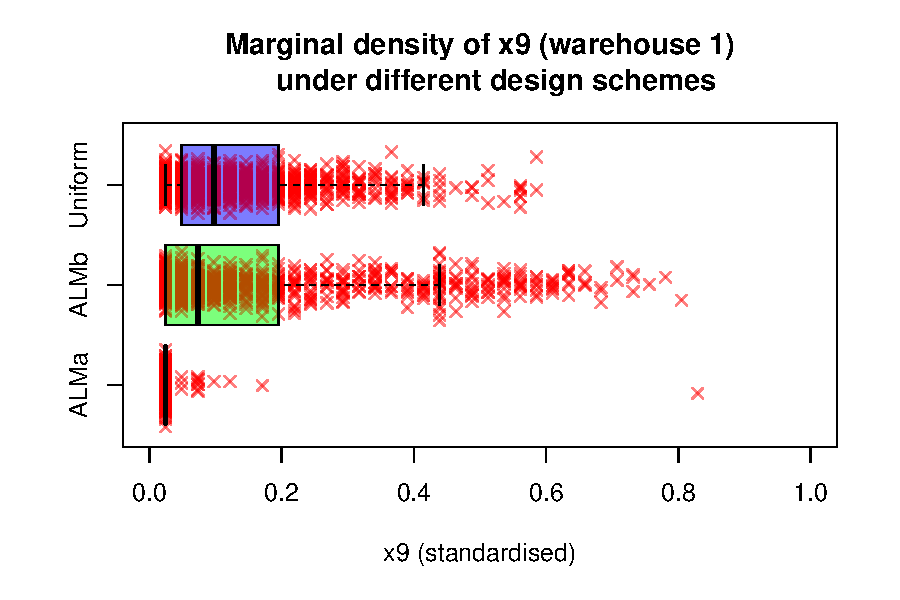
\includegraphics{fig-ds/compare-x9.pdf}
 \caption{Boxplots depicting the marginal density of $x_9$, for warehouse $1$, under three different design schemes. ALMa is the ALM design with the mean included, ALMb is the ALM design with no mean and Uniform is a uniform design generated by slice sampling. The red crosses denotes the values of $x_9$ from each design; these points are jittered vertically to aid visualisation. \label{Fig:compare-x9}}
\end{figure}
\begin{figure}
 \centering
 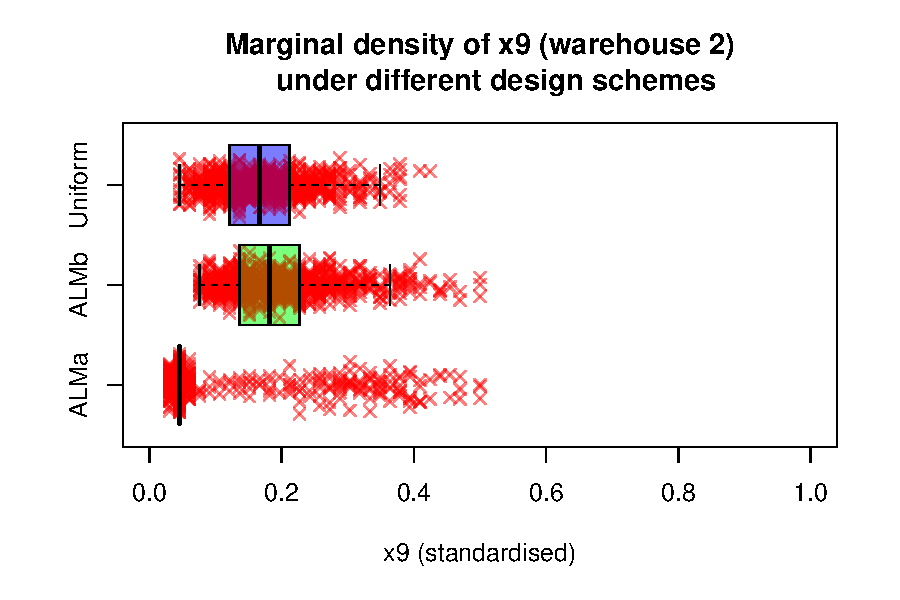
\includegraphics{fig-ds/compare-x9-w2.pdf}
 \caption{Boxplots depicting the marginal density of $x_9$, for warehouse $2$, under three different design schemes. ALMa is the ALM design with the mean included, ALMb is the ALM design with no mean and Uniform is a uniform design generated by slice sampling. The red crosses denotes the values of $x_9$ from each design; these points are jittered to aid visualisation. \label{Fig:compare-x9-2}}
\end{figure}
\begin{figure}
 \centering
 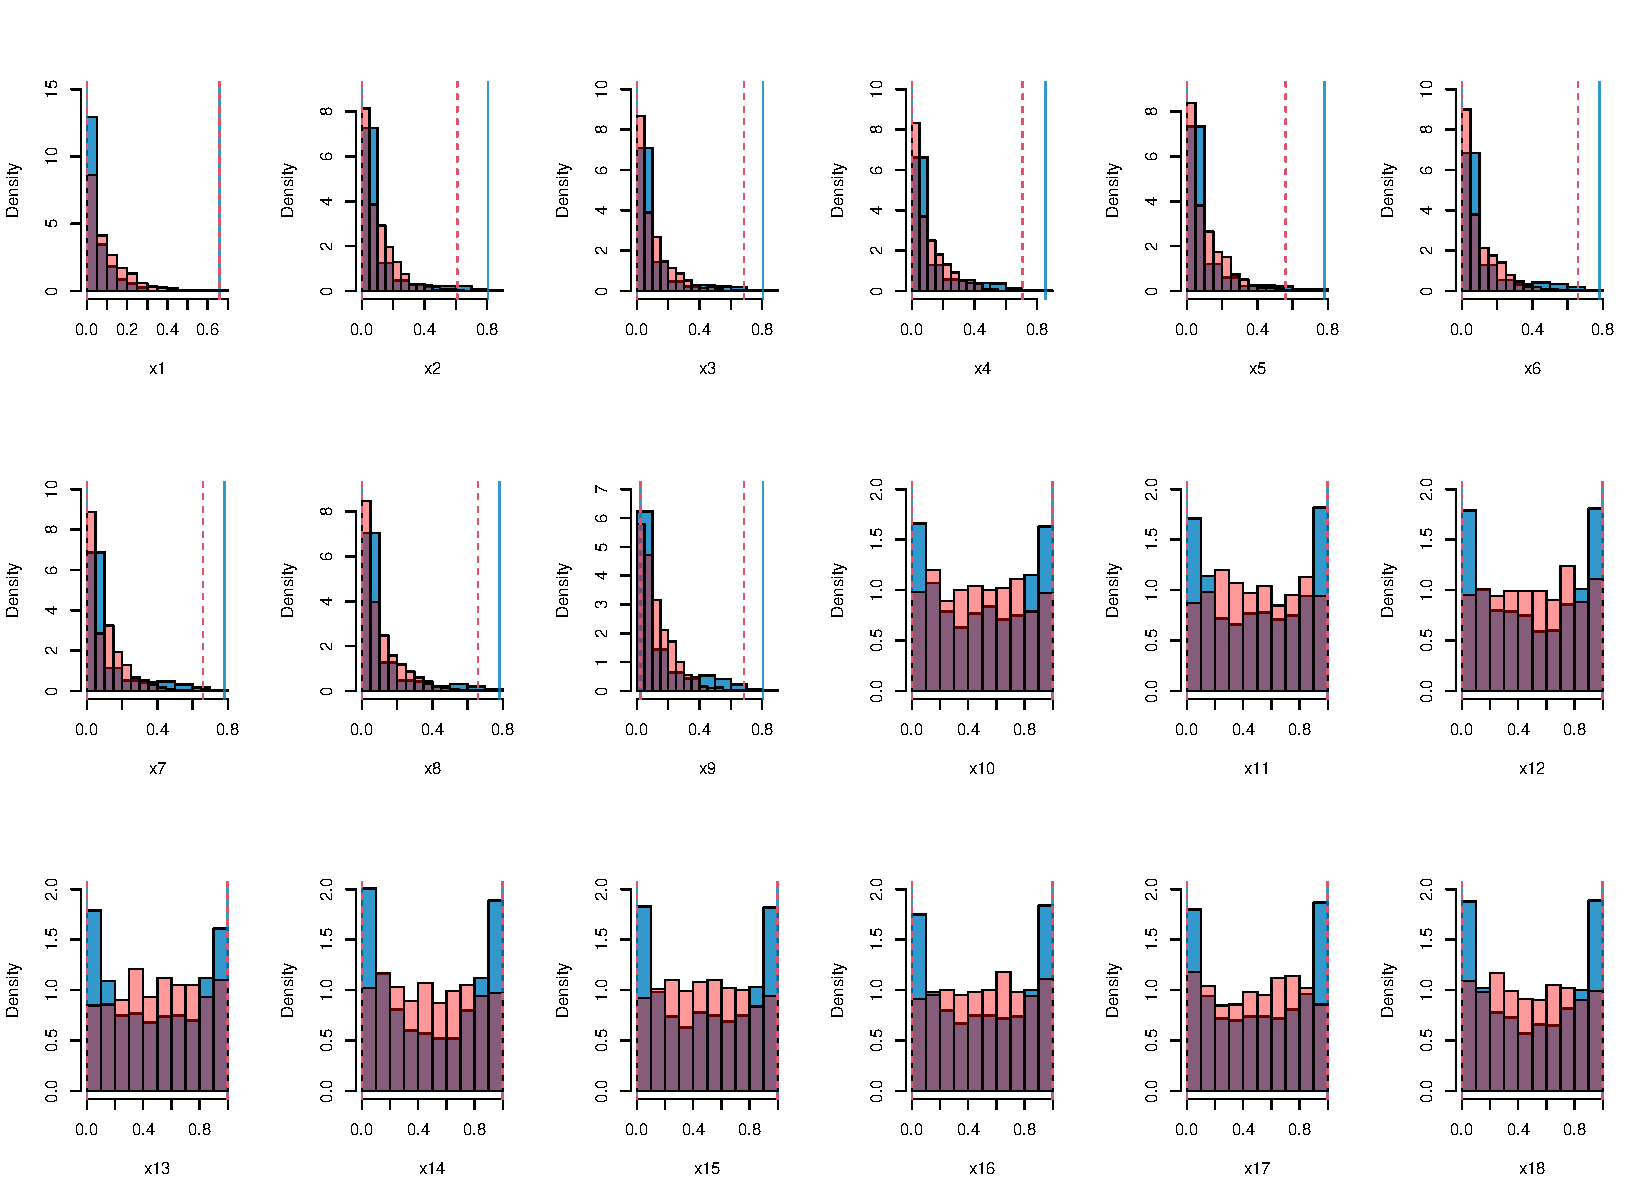
\includegraphics[width = 7.5in, angle = 90]{fig-ds/almnomean-vs-unif.pdf}
 \caption{Comparing the marginal behaviour of the ALM and the uniform designs for a sample size $n = 1000$ for Warehouse $1$. The ALM design is given as the blue histograms, whereas uniform are red. The limits of the ALM design are the solid blue lines, the dashed red lines are the limits of the uniform design.\label{Fig:alm-vs-unif}}
\end{figure}
\begin{figure}
 \centering
 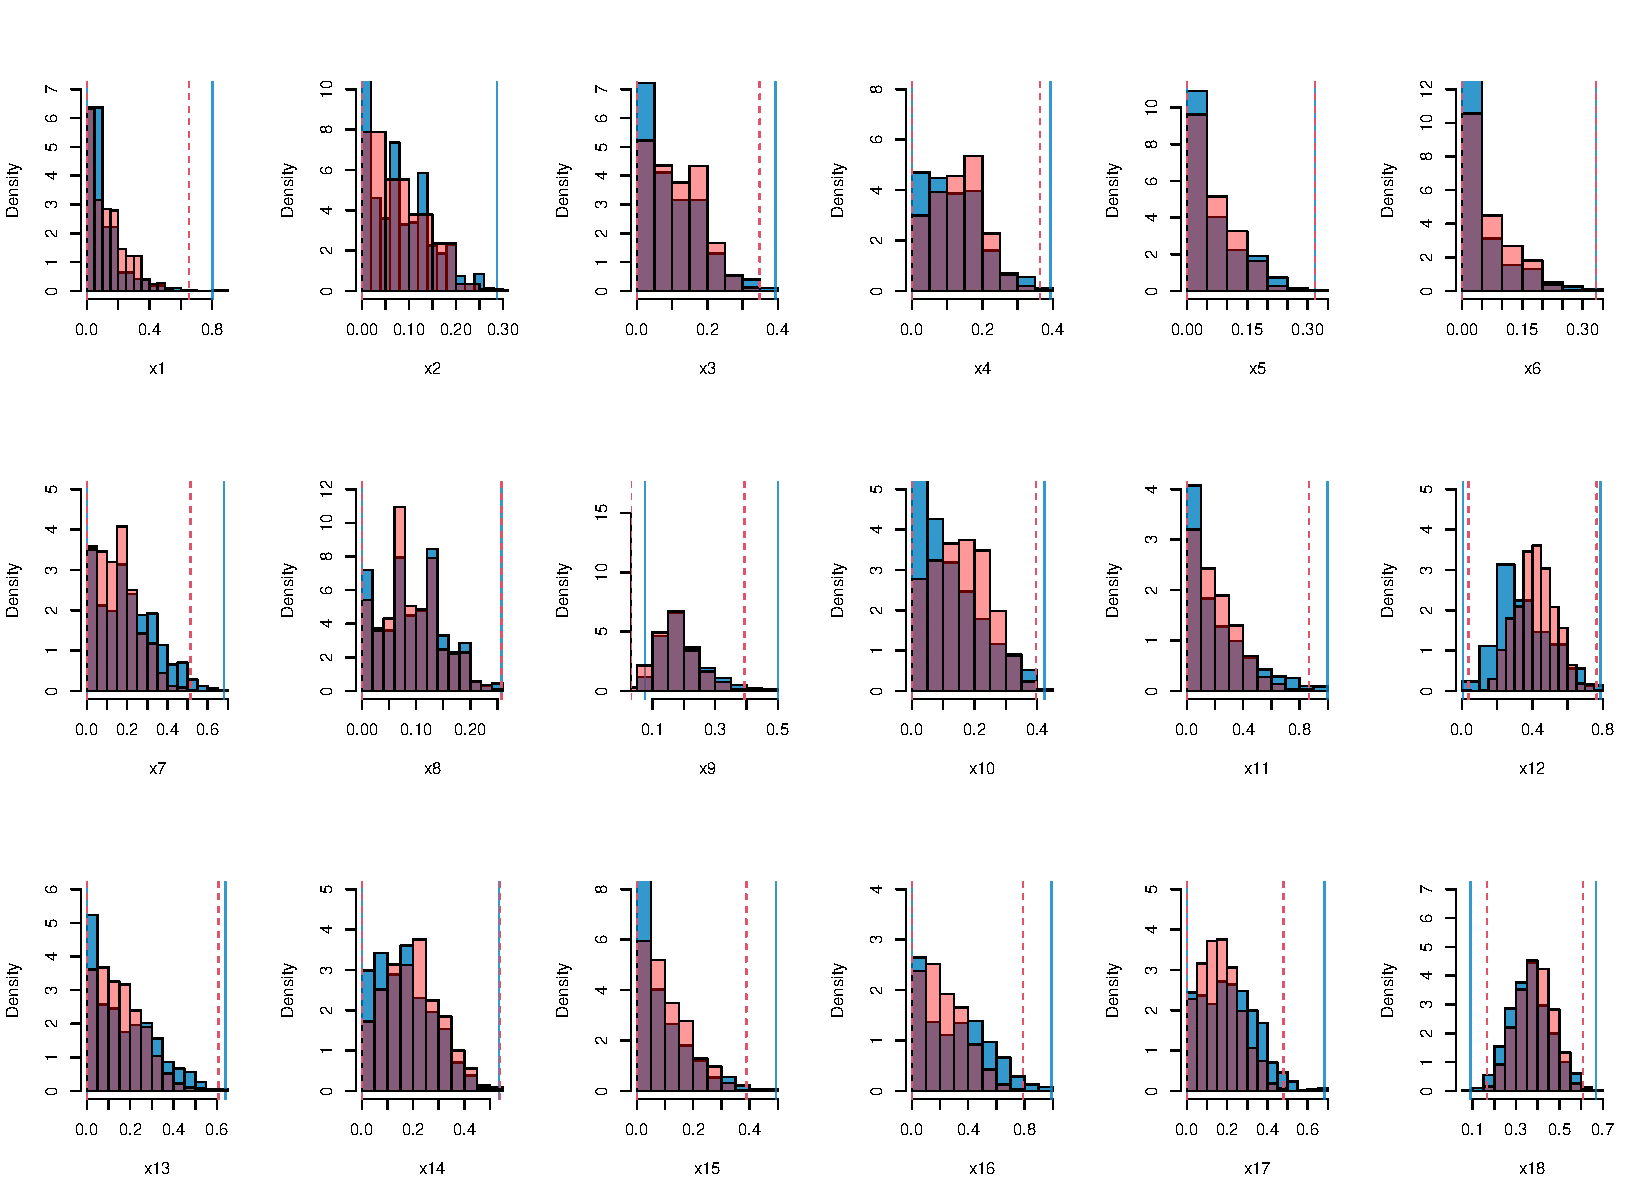
\includegraphics[width = 7.5in, angle = 90]{fig-ds/almnomean-vs-unif2.pdf}
 \caption{Comparing the marginal behaviour of the ALM and the uniform designs for a sample size $n = 1000$ for Warehouse $2$. The ALM design is given as the blue histograms, whereas uniform are red. The limits of the ALM design are the solid blue lines, the dashed red lines are the limits of the uniform design.\label{Fig:alm-vs-unif2}}
\end{figure}
\subsection{Wave $2$ emulators}

To construct the wave $2$ emulators we used the ALM designs discussed above. As with the wave $1$ emulators the training data is generated by averaging over $30$ realisations of $u(\bx)$ for each $\bx$.

For the GP hyperparameters, we adopted the same priors as the wave $1$ emulators, as these are relatively weak, but chosen to omit unrealistic values of the hyperparameters. We adopted the prior mean function $\mu(\bx) = \beta^{(i)}_0 + \beta^{(i)}_1 \log (x_9 + 10^{-8})$. The prior for each $\bm{\beta}^{(i)}$ was chosen as $\bm{\beta}^{(i)} \sim \pi(\bm{\beta} \mid \mathcal{D}^{(i)}, \Theta_i)$. That is, the posterior distributions from wave $1$ are adopted as wave $2$ prior distributions. We also tried including a more detailed mean function (and thus adjusted the prior on each $\beta^{(i)}$), however, we found that leave-one-out RMSE (\cref{Eq:rmse}) and Score (\cref{Eq:scoring-rule}) degraded when using a more detailed mean function. We therefore retain the functional form $\mu(\bx) = \beta^{(i)}_0 + \beta^{(i)}_1 \log (x_9 + 10^{-8}) $.
\begin{figure}
 \centering
 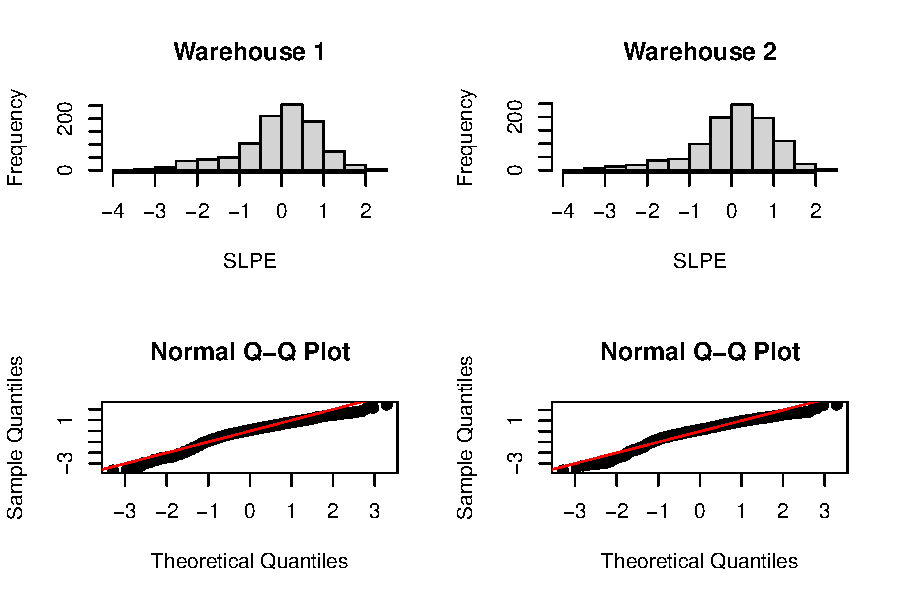
\includegraphics{fig-ds/diagnostics-wave2.pdf}
 \caption{Global diagnostics for the wave $2$ emulators. The left hand plots are for warehouse $1$ and the right hand for warehouse $2$. The top plots show histograms of LOO errors and the bottom plots are Normal QQ plots for the LOO errors.\label{Fig:w2-global-diag}}
\end{figure}
The emulators were fitted using our usual EB approach; assume a Normal likelihood, integrate out $\bm{\beta}^{(i)}$ and then finding a MAP estimate of the GP covariance structure. Global diagnostics are given in \cref{Fig:w2-global-diag}. We see there is some deviation from the Normality assumption. Namely, the left hand tail appears to be longer than the right hand tail. The excessive number of large, negative residuals implies there is some systematic under-prediction. This means the proportion of decisions ruled out may be larger than the proportion that would have been ruled out under a `perfect' emulator. When considering the problem of optimisation under uncertainty, we would argue this is preferable to the opposite scenario of many under-predictions with large error, since systematic under-prediction would lead to the NROY space being smaller than it should be. That is, we would be ruling out decisions that should be retained. Since this approach is conservative and aims to address uncertainty, we would rather retain some sub-optimal decisions (be inefficient) than rule out potentially good decisions (be ruthless). Plots of SLPEs against each inputs, for both warehouses, are given in \cref{App:resid3}.

However, the mean SLPE for warehouse $1$ is $-0.0452$ and the mean SLPE for warehouse $2$ is $0.00757$ which suggests that the SLPEs are not biased away from $0$. Moreover, we see that the observed proportions of SLPEs within $\pm2$ and $\pm3$ are close to their theoretical proportions, assuming Normality (\cref{Tab:cred2}). The observed proportions are slightly under the theoretical proportions, however, there is agreement with Pukelsheim's $3\sigma$ rule so we can perform another round of iterative refocussing with confidence in the calibration of the approach.
\begin{table}
 \centering
 \begin{tabular}{rrrr}
  \toprule
  Warehouse & SLPE Interval & Expected Proportion & Observed Proportion \\\cmidrule{1-4}
  $1$ & $(-2,2)$&$0.95$ & $0.944$\\
  &$(-3,3)$& $0.997$ & $0.995$ \\\cmidrule{1-4}
  $2$ & $(-2,2)$&$0.95$ & $0.954$\\
  &$(-3,3)$& $0.997$ & $0.992$ \\\bottomrule
 \end{tabular}
 \caption{Comparing the expected proportion to the observed proportion of SLPEs to lie within given intervals, assuming Normality of the SLPEs for the wave $2$ emulators.}
 \label{Tab:cred2}
\end{table}
\subsection{What is the maximiser?}
Although our philosophy towards decision making views the problem as having a set of sensible solutions, rather than one optimal solution, the HM inspired approach still needs a `best' value to rule out decisions. If our simulator was deterministic, we would simply take the largest value seen so far. However, we are working with a stochastic simulator. The uncertainty about the largest expected utility is an additional complication.

After the first wave, taking the largest expected utility, amongst the design points, is a natural choice for `best'. However, the wave $2$ emulators offer a new perspective of $U(\bx)$. The purpose of the wave $2$ emulator is to explore a diverse set of decisions (via an ALM design) rather than to exploit knowledge of $U(\bx)$ to optimise it. Since the wave $2$ emulator was not designed to optimise $U(\bx)$, should we trust its maximiser?

If we plug $\hat{\bx}_1$ into the wave $2$ emulator, we obtain $U(\hat{\bx}_1) \sim \mathcal{N}(0.790, 2.54\times10^{-4})$ which is rather different from the wave $1$ prediction. This is troublesome as it is not clear how to define our implausibility measure, which is reliant on the distribution of $U(\bx)$, and how it is correlated with $U(\bx')$. However, $\tfrac{|0.790 - 0.831|}{\sqrt{2.54\times10^{-4} + 8.75\times 10^{-5}}} = 2.22 < 3$ so these two characterisations of uncertainty about $U(\hat{\bx}_1)$ are in some sense compatible with each other. If we search the wave $2$ design, the largest expected utility belongs to warehouse $1$ and is characterised by
\begin{equation}
 U(\hat{\bx}_2) \sim \mathcal{N}(0.818, 2.47 \times 10^{-4}).
\end{equation}
Now, $\E \{ U(\hat{\bx}_2) \}$ is much closer to $\E\{U(\hat{\bx}_1)\}$; note that $|\tfrac{(0.831 - 0.818)}{\sqrt{8.75 \times 10^{-5} + 2.47 \times 10^{-4}}} | = 0.725$, thus relative to their uncertainties, these two characterisations of the optimum value are fairly close.
One solution to this problem is to perform sensitivity analysis: perform the analysis for both potential maximisers and see how different the results are. To perform the sensitivity analysis we will use $\hat{\bx}_1$ and take our uncertainty about $\hat{\bx}_1$ as characterised by the wave $1$ emulator. Our uncertainty about $\hat{\bx}_2$ will be characterised by the wave $2$ emulator.

This means there will be two possible implausibility measures. They are, for $\bx \in \calX_2$
\begin{align}
 I_{2,1}(\bx) &= \frac{\E^{(1)}\{U(\hat{\bx}_1)\} - \E^{(2)} \{U(\bx)\} }{\sqrt{\var^{(1)} \{U(\hat{\bx}) \} + \var^{(2)}\{U(\bx)\} }}\\
 I_{2,2}(\bx) &= \frac{\E^{(2)}\{U(\hat{\bx}_2)\} - \E^{(2)} \{U(\bx)\} }{\sqrt{\var^{(2)} \{U(\hat{\bx}) - U(\bx)\} }}
\end{align}
where the $(j)$ superscript denotes the expectation/variance at the $j$th wave of emulation. The $i,j$ subscript denotes that this is the implausibility at wave $i$ and we are using $\hat{\bx}_j$ as the `reference' value for HM.

\subsection{Second round of refocussing}
\begin{table}
	\centering
	\begin{tabular}{llrr}
		\toprule
  Wave & Best value & \multicolumn{2}{c}{Warehouse} \\\cmidrule{1-4}
  Wave $2$ only& & $1$ & $2$ \\
  &$\hat{\bx}_1$ & $50.5\%$ & $99\%$ \\
  &$\hat{\bx}_2$ & $90.8\%$ & $100\%$\\\cmidrule{1-4}
  Both waves& & $1$ & $2$ \\
  &$\hat{\bx}_1$ & $45.89\%$ & $1.39\times10^{-3}\%$ \\
  &$\hat{\bx}_2$ & $82.51\%$ & $1.40\times10^{-3}\%$ \\\bottomrule
	\end{tabular}
	\caption{Estimated proportion of the decision space remaining for each warehouse. The top half of the table is the reduction in space due to the wave $2$ emulators, having already reduced the space by wave $1$ emulators; the bottom half is the total reduction in NROY space from both waves of emulation. \label{Tab:compare-nroy}}
\end{table}
To assess the reduction in the NROY space we first use $I_{2,1}(\bx)$ as an implausibility measure. We will then use $I_{2,2}(\bx)$. Both measures will use the cut off of $3$ to determine which points have been ruled out. To estimate the reduction in the NROY space (compared to the previous wave) we will use a random, uniform sample of $1000$ points which were deemed not implausible after the first wave of emulation. The reduction in NROY space for each warehouse, using the different implausibility measures, is given in \cref{Tab:compare-nroy}. Using $\hat{\bx}_2$ as the maximiser leaves the NROY space essentially unchanged; it offers no reduction whatsoever in the space of warehouse $2$ and removes under $10\%$ of the space for warehouse $1$. When using $\hat{\bx}_1$ as the maximiser, we obtain a modest reduction in NROY space for warehouse $1$ and a small reduction in the space for warehouse $2$.

We will use $\hat{\bx}_2$ as the maximiser since it represents our current understanding of $U(\bx)$. This does not reduce the NROY space, which is somewhat frustrating. However, we should not to rule out decisions solely for the sake of ruling out decisions. This poses a question; since $\E\{U(\hat{\bx})\}$ has decreased, and $\var\{U(\hat{\bx})\}$ has increased, should we go back a wave and re-introduce decisions that were ruled out? We will not do this, but, \citet{baker-thesis2021} considers the notion of a flexible NROY space and shows that allowing the NROY region to shrink as well as grow protects against flaws in emulators from early waves. \citet{baker-thesis2021} shows, for a small set of simple examples, that the flexible approach can be advantageous in finding the `correct' NROY space.
\subsection{Termination of iterative refocussing}
After performing these two waves of analysis, we have used, approximately, a total of $22 \text{ cores} \times 5 \text{ training rounds} \times 6 \text{ days } \approx 1.8 \text{ years}$ of CPU time on generating training data for the emulators. This is based on the assumption that running Athena at $1000$ inputs, each replicated $30$ times, will take $6$ days (over $22$ cores). Training runs of Athena for this analysis took in the region of $5$-$7$ days, therefore $6$ days is a reasonable approximation. There is also the issue of queuing on HPC facilities which can be of the order of several days during busy periods. In terms of wall-clock time, we used a total of around $14$ days computing time. Another round of emulation would take approximately another $6$ days in training time. None of our calculations have included the human time required to perform analyses, the computational cost of fitting and validating of emulators or the computational cost of a design. For this reason, combined with the very small reduction in the NROY space we now terminate our iterative procedure.

Since we have terminated our procedure, we can calculate what proportion of decisions are NROY compared to the original set. This quantity is given by
\begin{align*}
 |\calX_{\text{NROY}}| &= \frac{0.8251 \times {49 \choose 8} + 1.39 \times 10^{-6} \times {74 \choose 8} + 0 \times {99 \choose 8}}{{49 \choose 8} + {74 \choose 8} + {99 \choose 8}}\\
 &= \frac{3.72 \times 10^8}{1.87 \times 10^{11}}\\
 &= 1.99 \times 10^{-3}
\end{align*}
which is a reasonable reduction in the size of the NROY volume; around $0.2\%$ of the original decisions have been deemed NROY. Note that we have completely ruled out warehouse $3$, and the number of decisions remaining from warehouse $2$ is tiny. Most of our remaining decisions correspond to warehouse $1$. By ruling out many decisions, we have greatly simplified the problem for the DM.
\section{Incorporating the DM: evaluating the consequences of decisions}
The final aspect of our analysis contains two parts. First we will provide the DM with a small set of NROY decisions. Displaying the consequences of a large set may overwhelm the DM and thus they may not be able to adequately assess the relative merits of each decision. These are decisions which are not clearly worse than $\hat{\bx}_2$. For each decision put forward to the DM, we will present the decision alongside the consequences of that decision. Recall, the consequences are the choice of warehouse, the availability time series and the restoration policy. We will present many replicates of the availability times series to the DM to communicate that this is an uncertain consequence.

The DM then has two tasks. The first task is to provide feedback on the decision space. If the DM finds believes that the given decisions are not consistent with their preferences, we must go back to the start of our analysis and perform the entire task again; re-elicit attributes, consequences, the functional form and parameters of the utility function \citep{Smith2010}. However, this is very computationally expensive so, if the DM does reject all of the decisions shown, we could first present a new sample of decisions. Note that this step is computationally expensive because one consequence relies on running the Athena simulator. However around $30$ replicates for a small handful of decisions can be computed in about an hour on the Rocket HPC facility, or overnight on a modern desktop computer. If the DM is not satisfied, it may be worth trying to optimise a single consequence. For example, if the DM was not happy with the availability trajectories we have produced from the NROY space, it would be worth investigating if there are \textit{any} availability trajectories within the initial decision space that the DM is happy with. We should also remind ourselves that decision analysis allows us to make the best decision, however, it is entirely possible that there are no `good' decisions, but rather, we must find the least worst option. For example, suppose you must make a long journey. You can either take the train, which takes $12$ hours and involves multiple connections, or you can take a $1$ hour flight. Further suppose you are environmentally conscious, and are aware that taking a flight is much more harmful to the environment than the train. Both decisions have obvious disadvantages and you might be unhappy with both prospects, but there will still be an optimal decision.

If the DM finds one or more solutions satisfactory, they must then decide which decision to make. This decision should solely be that of the DM.
\subsection{Presenting NROY decisions to the DM}
Since no real DM is involved in the analysis, we chose a set of $12$ decisions to present to our fictitious DM; $6$ from each warehouse. One was chosen as $\hat{\bx}_2$, another was chosen as the decision which maximised the wave $2$, warehouse $2$ emulator and a further $5$ random decisions from each warehouse within the NROY set. The values of $x_{1}$ -- $x_{18}$ for each of these decisions is given in \cref{Tab:final-dec}. The first $6$ decisions corresponds to warehouse $1$ decisions, the final $6$ to warehouse $2$. The $6$th decision is $\hat{\bx}_2$ and the $12$th decision is the decision which maximised the wave $2$, warehouse $2$ emulator. If a DM were to be involved, they may request the analyst to further investigate particular decisions, provided they are NROY.

We ran the Athena simulator $300$ times at each of these input configurations to give the DM a detailed picture of the availability trajectories one could see if we made any of these $12$ decisions. Allowing the DM to choose one of these decisions for themselves has the advantage of allowing the DM to bring in any additional information that was not given to the analyst. This ensures that the DM's preferences are honoured if the elicited utility function is a misrepresentation of their beliefs.
\begin{figure}
 \centering
 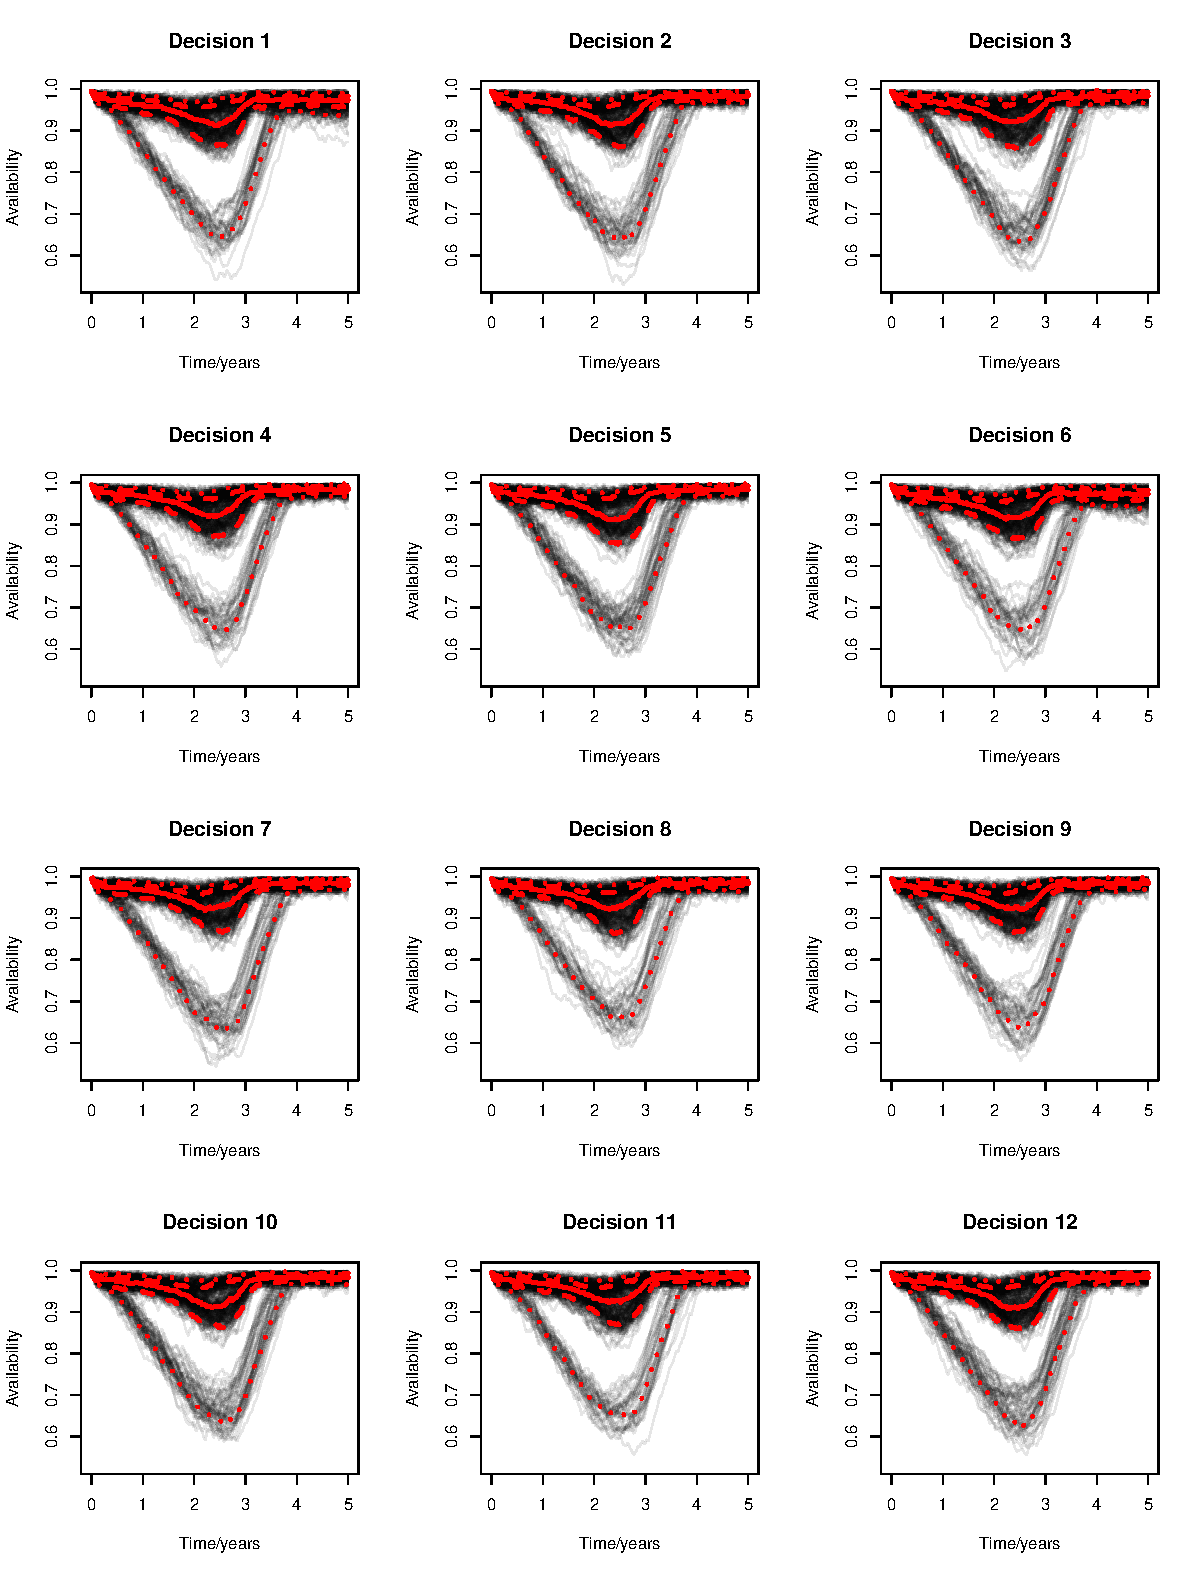
\includegraphics[width=\textwidth]{fig-ds/final-decisions-bold.pdf}
 \caption{Each sub-figure shows $300$ availability trajectories (grey lines) for each of the decisions given in \cref{Tab:consequences}. The solid red line represents the median availability trajectory for a decision, the dashed red lines correspond to $20\%$ and $80\%$ quantiles for the availability and the dotted red lines represent $5\%$ and $95\%$ quantiles for the availability. Quantiles are all point-wise.\label{Fig:final-avail}}
\end{figure}
\begin{sidewaystable}
\centering
\pgfplotstabletypeset[
multicolumn names,
col sep = comma ,
string type ,
every head row/.style ={ %
before row ={ %
\toprule
& \multicolumn{18}{c}{Decision variable ($x_i$)}\\
\cmidrule{2-19}\\
} ,
after row ={\midrule}
} ,
every last row/.style={after row =\bottomrule}
] %
{code-for-plots/sensible-decisions2.csv}
\caption{The values of $x_1$--$x_{18}$ for each of the $12$ decisions presented to the DM. Note that the first $6$ decisions correspond to warehouse $1$ ($x_{19} = 50$) and the final $6$ corresponds to warehouse $2$ ($x_{19} = 75$).\label{Tab:final-dec}}
\end{sidewaystable}
In \cref{Fig:final-avail} we see that the distribution of availability trajectories is very similar for the $12$ examples. By eye, it is essentially impossible to tell them apart. Each set of trajectories seems to have two modes. The `main' mode has the availability trajectories typically sitting in the region of $[0.9,1]$ for all $\text{Time} \in [0,5] \text{ years}$. The `minor' mode has a prominent dip in availability in for when Time is in the region of $[2,3]$ years; the availability drops to a minimum which is typically in the range $[0.6, 0.7]$.
\subsection{Retrospective validation of assumptions}
We now wish to (retrospectively) verify three aspects of our analysis. Our maximin design was constructed from, essentially, one long run of \cref{alg:nroy-disc}, rather than the ergodic variant --- we need to check that the Markov chain is irreducible (that is, not ergodic). Next, we relied on Pukelsheim's $3\sigma$ rule to determine which decisions are (not) consistent with the (estimated) optimal decision. We can only use Pukelsheim's $3\sigma$ rule when $U(\bx)$ has a continuous, unimodal distribution; we should verify this assumption. Finally, we should check that decisions from the final NROY set are indeed consistent with our findings.

\subsubsection{Checking the Markov Chain is irreducible}

To verify that the Markov chain used to generate a large candidate design is indeed irreducible, we implement \cref{alg:ergodic-disc-slice} with $R=30$ repeated runs, $n' = 1000$ within-chain runs for a total sample size of $N = 30000$. This is performed for each of warehouses 1 and 2.

To investigate as to whether or not the chain is reducible, we first performed principal components analysis to obtain a low-dimensional visualisation of the NROY samples. The first two principal components are shown for the two samples of $N = 30000$ NROY points generated from \cref{alg:ergodic-disc-slice} are shown in \cref{Fig:check-ergodic}.

\begin{figure}
  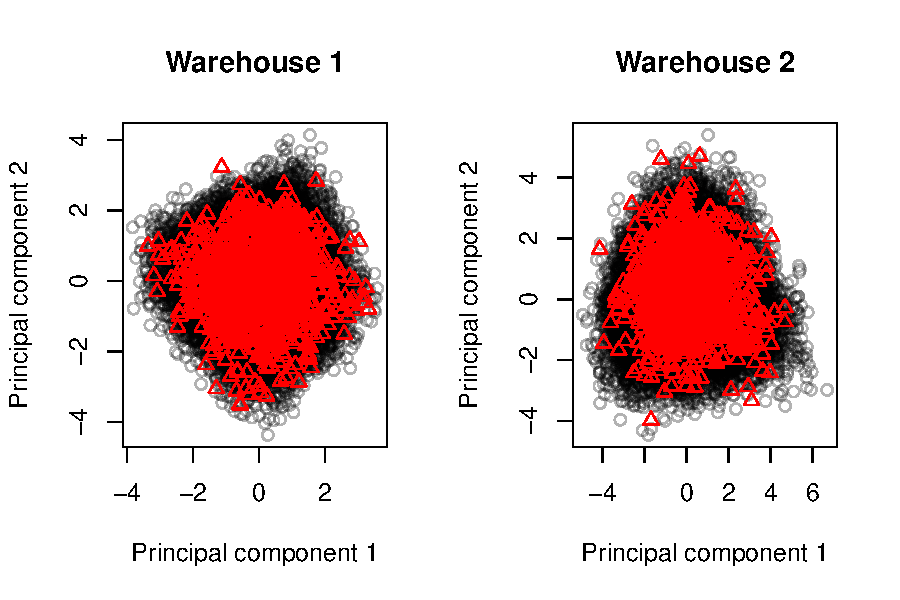
\includegraphics[width = \textwidth]{fig-ds/check-ergodic.pdf}
  \caption{For each warehouse, the figures show the first two principal components of a large collection of uniform NROY samples. The black circles are points from all chains, whereas the red triangles are a all the points from just one of the parallel runs. We see in both cases, that there is no evidence of a disconnected NROY region.\label{Fig:check-ergodic}}
\end{figure}

In each of the subfigures of \cref{Fig:check-ergodic}, there is no evidence to suggest that the NROY region is a union of disconnected regions. The red triangles --- the points from just one of the parallel runs --- have a similar joint distribution to all other samples. Further, the samples all appear to come from one connected region, rather than two or more disconnected sub-regions. Note that these samples are uniform across the NROY region and not processed to form (e.g.) a maximin design.

\subsubsection{Pukelsheim's $3\sigma$ rule}
Our history matching procedure has relied on Pukelsheim's 3$\sigma$ rule which states that $P(|U(\bx) - \mu| > 3\sigma) < 0.05$ under two assumptions. Firstly, $U(\bx)$ must be continuous. This is satisfied as $u(\bx)$ is a smooth function of $\bx$ and availability is a continuous-valued random quantity. The second assumption is that $U(\bx)$ must be unimodal. The sub-figures within \cref{Fig:final-avail} all show that the availability distribution has at least two modes. By the CLT, we would expect our training outputs, $y(\bx)$, to be approximately Normal (and thus unimodal) as they are constructed via sample means. However, it is important to remember that the CLT is only an asymptotic result and offers no general guarantee for samples sizes $n < \infty$. To verify that the training data are unimodal quantities, we perform a simple bootstrap procedure to estimate the sampling distribution of $y(\bx) = (1/30) \sum_{i=1}^{30} u(\bx)_i$.
\begin{figure}
 \centering
 \includegraphics{fig-ds/bootstrap.pdf}
 \caption{Bootstrap distributions for $4$ randomly chosen inputs, $\bx_i$, $i = 1, 2, 3, 4$, from the wave $2$ design. The bootstrap distribution for $y(\bx_i)$ is based on $1000$ values of $y(\bx_i)$. \label{Fig:bootstrap}}
\end{figure}
The bootstrap distributions shown in \cref{Fig:bootstrap} all support the assumption that $y(\bx)$ is unimodal, even though $u(\bx_i)$ has a multimodal distribution. Note that, if $y(\bx)$ was still multimodal, the methodology we used would not work. To remedy this, we can increase the sample size which $y(\bx)$ are based on. This will mean that training data are more expensive to obtain; the benefit is that we can avoid many awkward probability distributions and thus utilise relatively simple and robust methods to quantity uncertainty about $U(\bx)$.
\subsubsection{Consistency of final NROY volume}
To check that the final NROY volume is indeed consistent with our uncertainty about the optimal decision, we can re-use the large samples presented in \cref{Fig:final-avail}. In particular, the $300$ samples shown in each sub-figure are random draws which are independent of any emulator training data and the emulators themselves. The means and standard errors implied by these samples offer an independent perspective of $U(\bx)$ for each $\bx$. Comparing these to the emulator's characterisation of $U(\hat{\bx}_2)$ allows us to assess if the apparently NROY decisions should have been ruled out.
\begin{table}
\centering
\begin{tabular}{rrrr}
 \toprule
 Decision & $\widehat{U}(\bx)$ & $\widehat{\text{s.e.}}(\bx)$ & $I^{*}(\bx)$ \\\cmidrule{1-4}
 1 & $0.788$ & $5.592\times 10^{-3}$ & $1.801$ \\
  2 & $0.786$ & $6.138\times 10^{-3}$ & $1.897$ \\
  3 & $0.806$ & $6.254\times 10^{-3}$ & $0.739$ \\
  4 & $0.797$ & $5.832\times 10^{-3}$ & $1.281$ \\
  5 & $0.793$ & $6.326\times 10^{-3}$ & $1.484$ \\
  6 & $0.800$ & $5.414\times 10^{-3}$ & $1.071$ \\
  7 & $0.789$ & $6.244\times 10^{-3}$ & $1.728$ \\
  8 & $0.801$ & $5.657\times 10^{-3}$ & $1.053$ \\
  9 & $0.799$ & $5.978\times 10^{-3}$ & $1.139$ \\
  10 & $0.791$ & $6.406\times 10^{-3}$ & $1.614$ \\
  11 & $0.807$ & $5.708\times 10^{-3}$ & $0.693$ \\
  12 & $0.788$ & $6.317\times 10^{-3}$ & $1.797$ \\\bottomrule
\end{tabular}
\caption{Means ($\widehat{U}$) and standard errors ($\widehat{\text{s.e.}}$) for the expected utility of the $12$ decisions corresponding to \cref{Fig:final-avail} and \cref{Tab:final-dec}, as well as an implausibility measure ($I^{*}$) for each decision. \label{Tab:final-dec-implaus} }
\end{table}
\cref{Tab:final-dec-implaus} shows the mean and standard error for each of the $6$ decisions given in \cref{Fig:final-avail}. Our implausibility measure for this final aspect of the analysis will be
\begin{equation}
 I^{*}(\bx) = \frac{\E\{U(\hat{\bx}_1)\} - \hat{U}(\bx_i) }{ \sqrt{ \var\{U(\hat{\bx}_1)\} + \widehat{ \text{s.e.} }\{\hat{U}(\bx_i)\}^2 }\ }
\end{equation}
where $\widehat{ \text{s.e.} }\{\hat{U}(\bx_i)\}$ is the estimated standard error of $\hat{U}(\bx_i)$. Recall that $\bx_6 = \hat{\bx}_2$. In this case we see that $0$ decisions are ruled out under $I^{*}$. Under Pukelsheim's $3\sigma$ rule we would expect to retain \textit{at least} $90\%$ of decisions after two well-calibrated waves. Assuming Normality (and a cut off of $3$) we would expect to retain around $98\%$ of decisions after two well-calibrated waves. This sample size is small but $100\%$ is close enough to $98\%$, and clearly $100\% > 90\%$, we therefore judge that our ruling out procedure is well-calibrated.

\section{Discussion}

We have presented a history matching inspired procedure for decision support with the stochastic Athena simulator. Our approach drew on established ideas, such as the UCB BayesOpt heuristic \citep{Srinivas2009} and history-matching inspired decision support for deterministic simulators \citep{Owen2020} but relied on novel applications of these ideas to address the challenges within our applied problem of decision support under uncertainty for the Athena simulator.

We first provided an illustrative elicitation of a utility function. We drew on key attributes to the problem, but we stress the elicitation will always be subjective; every DM has their own utility function.

We then proposed unifying two established approaches. We began by performing three independent rounds of BayesOpt to optimise the choices of $x_1$--$x_{18}$ then used techniques from the HM literature to communicate uncertainty about the optimal decision. Our HM inspired approach required a novel implausibility measure which accounts for dependence across the decision space.

We then considered the design for our decision support exercise. Since a subset of our inputs were a discrete simplex, which is non-standard in the computer experiments literature, this posed some interesting challenges. BayesOpt allowed us to side-step the problem of design for a wave $1$ emulator since it automatically chooses where to run the simulator. The design for a wave $2$ emulator was more challenging as we had to adhere to the constraints of the decision task a whilst constructing a design within the NROY region that provided a diverse set of decisions. Sequential design offered a promising approach again. Our approximate ALM design allowed us to construct a design which was more space-filling than a uniform design. We believe sequential designs are a promising option for non-standard input spaces.

We then constructed a new pair of emulators to further explore the NROY space. We performed a sensitivity analysis based on the choice of possible maxima. One maximum led to a negligible reduction in the NROY space and the other led to a small reduction in the NROY space. In general, we would advise using the results of the most recent emulator to choose the maximiser (when $y(\bx)$ is stochastic). This would protect against $U(\hat{\bx})$ being an over-estimate, which may rule out too many decisions. In the deterministic case, it would be natural to choose the largest observed value across all waves.

Next we presented the DM with a set of sensible decisions that could be taken. We presented decisions from both warehouses and from diverse decisions within each warehouse.

Finally, we performed some post-hoc checks to verify some assumptions, as well as checking whether the proportion of incorrectly ruled out decisions is consistent with Pukelsheim's $3\sigma$ rule. Our small sample of decisions suggested that we did not rule out too many decisions, although a much larger sample would be needed to make a conclusive statement.

If we were to perform the analysis again, with the assistance of a DM, we could prevent ruling out too many decisions by incorporating model discrepancy. It would be possible to estimate model discrepancy via the elicitation procedure. When fitting the utility function to the DM's beliefs, we could use the `over-fitting' technique in which we elicit more preferences than necessary. We can then fit a functional form to the elicited quantities via least squares. The sum of squares will be positive and can be interpreted as a variance. This sum of squares can be used as a \textit{minimum} model discrepancy. Nonetheless, even if we did rule out too many decisions, commonly used approaches would have only provided one decision. Thus, we have been successful in \textit{supporting} decision making, rather than making the decision on behalf of the DM.

Another avenue for further investigation would be simulation experiments to learn about various aspects of our approach. \correction{Firstly, we are not aware of any simulation experiments which address how often a history matching based approach will rule out the `true' maximiser. In part, this gap in the literature will be due to the complexities of HM. Describing an NROY region is only practically possible by testing whether points are in the NROY region or not.  We do not consider this to be a problem for this work as HM delivers what we need: a greatly reduced decision space from which a DM can choose a good --- not necessarily optimal --- decision.}

Another aspect which would benefit from further investigation would be the choice of design. We pragmatically chose to use an ALM design based on (a) the range of the NROY volume covered by the design and (b) the theory behind ALM designs which suggests points should be spread apart, so we are considering `diverse' decisions. It would be interesting to see if there is any \textit{numerical} evidence to suggest that this approach is better, or indeed, worse than other methods. We would also like to investigate whether integrating the BayesOpt routine improved the history matching inspired approach. This would be in contrast to \citet{Owen2020} who used one shot designs for every wave of emulation, including the first, which may have allowed for greater exploration.

In terms of the decision problem, we considered a static policy in the sense that the decision variables do not change with time. However, many approaches within \citet{Tusar2022} were dynamic policies. We could consider two forms of dynamic policy: those which change with time, or those which change as data arrives (for example, updating prior beliefs with data, then maximising the DM's utility function with respect to a posterior distribution). A dynamic policy is where $\bx$ is replaced with $\bx(t)$, a vector-valued function of time. If $\bx$ is replaced by $\bx(t)$, the decision problem could be of a much higher dimension than our problem which has $17$ degrees of freedom. HM is an effective approach even in very high dimensional settings, for example \citet{White2018} uses HM to find plausible values for around $2500$ inputs. We imagine the methodology used in this chapter and used by \citet{Lawson2016} and \citet{Owen2020} could be successfully applied in other high dimensional settings. If the policy is dynamic in the sense that beliefs are being updated constantly or periodically, we would use exactly the same approach as above, with the addition that the procedure is run according to a pre-defined schedule. This would allow the DM to revise their utility function if aspects of the problem had changed. For example, the Athena simulator could be revised to offer an improved reflection of reality, or the DM may wish to update their utility function to incorporate new concerns. A dynamic policy however may not be suited to warehouse choice, but rather updating how we run a given warehouse.
\end{chapter}

  \begin{chapter}{Conclusion \label{Ch:conclusions}}

The goal of this thesis was to contribute to the toolkit of the subjective Bayesian; in particular we wished to reduce the computational burden of problems a subjective Bayesian may encounter when working with complex, stochastic simulators.

The contributions of this thesis were application-driven; we considered two problems within an offshore wind farm setting. The first problem was performing a meaningful sensitivity analysis so that a facilitator could prioritise the most important parameters for a SHELF elicitation workshop. This relied on constructing a data-hungry HetGP emulator. To improve the predictive properties of the HetGP emulators in a low-data regime, we developed and constructed the SML emulator. The next problem we considered was performing decision support so that a DM could devise a plan for managing a warehouse containing spare parts to be used when subassemblies suffer serious failures. The computational cost of each problem was greatly reduced by replacing the Athena simulator by suitably constructed emulators. Our emulators allowed us to perform decision support for stochastic simulators, we also considered sampling from NROY regions when the decision space is a discrete simplex.

\section{Thesis summary}
We began by introducing the Athena simulator and explaining some of its key components. The standard version of Athena overlooks the fact that spare components for key subassemblies may well be in limited supply. We therefore developed, and incorporated, some additional mechanisms which take into account that spare parts are difficult to obtain. We established that in situations where relevant data are difficult --- or even impossible --- to obtain, probability elicitation offers a practical solution to the problem of quantifying parameter uncertainty. We therefore discussed the SHELF; a framework for eliciting probability distributions which allows for, and encourages, the use of many experts for parameter elicitation. In a similar vein, when it is not clear what decision is optimal, we can elicit a utility function from a DM. This motivated our discussion of utility elicitation within the wider context of Bayesian decision analysis.

We then formally introduced the Gaussian Process, a stochastic process which naturally lends itself as a prior distribution for functions. The GP leads us to the notion of an emulator; a fast statistical surrogate model which produces a central prediction for a complex simulator with an appropriate quantification of uncertainty attached. We discussed a handful of common covariance functions and showed that (Bayesian) linear regression is linked to GP regression via linear covariance functions --- this fact can be used to improve the interpretability of emulators as the sum of two or more independent GPs is also a GP. We also discussed two other approaches to emulation. Linear regression offers a highly efficient (but perhaps less accurate) approach to emulation. Bayes linear approaches are also well suited to emulation; Bayes linear emulators are mathematically very similar to GPs, but offer a more robust analysis when we believe that a GP approximation of the simulator is too restrictive. These emulators are useful as they do not tie us to any probabilistic beliefs about how we expect an unknown function to behave. The catch is that, within a Bayes linear framework, we are limited in the types of statements we can make about unknowns.

We then explored methods for simultaneous mean and variance emulation. Simultaneous approaches, like HetGP, are more satisfying than the two-emulator approach \citep{Henderson09,Andrianakis2017} as we only need one surrogate for a single quantity of interest. A shortcoming of both of these types of models is that they require a lot of information to produce good quality emulators. This was avoided by the development of the SML emulator which exploited properties of Athena (the ability to run Athena at varying levels of complexity) to construct an improved emulator. We verified that the SML emulator offered an improvement by quantitative measures (RMSE and an appropriate scoring rule), as well as graphical diagnostics  suggesting a reduced emulator-simulator discrepancy under SML.

We then used our novel emulator to gain a deeper understanding of how a subset of the Athena simulator's parameters impact the output of the Athena simulator. We performed a probabalistic sensitivity analysis to see how changing the mean time to degradation impacted the distribution of the mean availability. We found that two parameters were responsible for the majority of the variation in the mean probit availability; the mean time to degradation for the turbine blades and the generator. The parameters were all of roughly equal importance for the variance component of Athena.

We then returned to decision analysis and reviewed various optimisation methods. Since the Athena simulator is computationally expensive, BayesOpt offered a promising solution to maximising a function of the outputs of the Athena simulator. In particular, BayesOpt allows us to maximise an expected utility function which depends on Athena. We also discussed that, because utility functions, elicited beliefs and models will always be imperfect representations of the objects they aim to represent, that allowing the analyst to make the decision, via performing mathematical optimisation, is myopic. The analyst in the problem should only \textit{support} the decision making process; it is up to the DM to make the decision. One way to do this is to employ history matching inspired techniques to construct a set of decisions which are, given all relevant and specified uncertainties, consistent with the maximiser. %In our case study we only have access to an approximate maximiser, so we found a set of decisions that were consistent with this approximate maximiser by considering the additional uncertainty about the approximate maximum value of the elicited utility function.

We then applied a novel combination of BayesOpt and history matching inspired methods to construct a set of decisions to aid a logistics problem. The Athena simulator featured in the problem by incorporating the availability time series into the elicited utility function. In our particular problem, we managed to greatly simplify the DM's decision by reducing the `big' warehouse decision down from a selection of $3$ warehouses to $2$. We also found decisions within each warehouse that were consistent with the approximate maximiser. Our volume of the final set of decisions was around $0.2\%$ of the size of the original decision space. The final set of decisions all lead to reasonably similar availability trajectories from the Athena simulator, which tells us that the DM can choose a warehouse and management policy from the final set of decisions that suits their preferences, without adversely affecting wind farm performance.

\section{Future research avenues}
\subsection{HetGP, SML and sensitivity analysis}
We showed that our novel SML emulator provided an improved emulator, over the benchmark HetGP, for our motivating Athena example at a fixed training budget. This allowed us to perform a sensitivity analysis to determine the relative importance of a subset of parameters to the Athena simulator.

The design for this example was chosen to be space filling, but beyond this, had no special properties. A promising avenue for future research would be developing designs which leverage our knowledge about the multiple levels of code.  Plainly, we should explore sequential designs. Although one `expensive' run may be computationally equivalent to $t$ `cheap' runs, it is not clear how informative cheap runs really are for expensive runs. Minimising some criterion, such as integrated mean squared prediction error, would allow the emulator to choose which of (i) a single expensive run or (ii) multiple cheap runs would be most useful for predicting the output of Athena (or some other simulator). This would also allow us to incorporate replication within the design. Replication is encouraged when emulating stochastic simulators with GPs since the cost and inference of GP modelling depends on the number of unique design \textit{locations}, $n$, rather than the total number of simulator runs, $N$. If $n << N$ then large computational savings are available due to the cubic/quadratic nature of GP calculations. This allows us to maximise the amount learned about $y(\cdot)$ whilst minimising the cost of implementing our emulators. Another idea that could be explored is incorporating more levels. The autoregressive function structure offers a natural way to incorporate many levels of code \citep{Kennedy2000}; we could also use this method to see which level of code is most time effective. Recall that an autoregressive model for functions takes the form
\begin{equation}
  f_{t+1}(\cdot) = \rho_{t} f_t(\cdot) + \delta_{t}(\cdot)
\end{equation}
where $t$ is a code level, $\rho_t$ is a regression parameter and $\delta_t(\cdot)$ is a discrepancy term. If $\delta_t(\cdot)$ is close to zero, and $\rho_t \approx 1$, then this suggests that $f_t(\bx) \approx f_{t+1}(\bx)$ and thus there is little advantage in using $f_{t+1}(\cdot)$ over $f_t(\cdot)$. The stochastic case should also consider if the output stochasticity is similar in the various code levels.

We would also like to consider ways to assess the joint impact of inputs on the simulator distribution. We mentioned in the discussion of \cref{Ch:sensitivity} that EVPI based methods would naturally allow for this when we have access to an appropriate utility function. Off the shelf utility functions, such as those based on the Kullback-Leibler divergence, may offer a good `default' when we are either unsure of what the utility function should be, or are interested in using the model for tasks such as parameter inference. Borrowing commonly used utility functions from the Bayesian design of experiments literature offers a promising start.

\subsection{Decision support: multiple stakeholders}

Using history matching techniques for decision support could be expanded to the case of multiple decision makers (typically termed ``stakeholders'') with different perspectives. Current approaches are somewhat limiting. For example, \citet{Keller2009} review several decision problems with multiple stakeholders. Typical solutions to decision problems with multiple stakeholders involve each stakeholder assigning a score to each possible decision by scoring the possible consequences, which are typically discrete in nature. Notably, such methods do not allow for any quantification of uncertainty about which decision is optimal, or the ability to clearly see whether the stakeholders can come to a compromise or not. Application of the single-stakeholder (a single DM) approach as in \cref{Ch:ds-for-ow} would generalise in a natural way.

Applying a history matching inspired approach, with $E$ stakeholders, we could construct $E$ sets of decisions that are consistent with the $e$th stakeholder's maximiser. Let these sets be $\calX_1,  \calX_2, \ldots, \calX_E$. The intersection of all these sets, $\calX^{*} = \bigcap_{e = 1}^E \calX_e$, is the set of mutually agreeable decisions; those that all stakeholders would be happy to take. Note that the DMs would not have to have the same set of attributes. If a DM, Alice, wanted to include $x_i$ in their analysis, but if a DM, Bob, did not want to include $x_i$, then we can just ensure that Bob's utility function is flat with respect to $x_i$. In an additive form, set $u_i(x_i)=0$, and for a multiplicative form set $u_i(x_i)=1$.

Although this is conceptually no more difficult than applying the approach to a single DM, there are computational and design issues that need to be considered. For example, when  constructing wave $k>1$ designs, we should investigate whether to  construct a design amongst the intersection of each decision maker's NROY set, and evaluate each DM's utility function \textit{only} at the intersection, or whether to construct a design amongst each DM's NROY set and evaluate each DM's utility function at their own set of NROY decisions. The advantage of the first approach is efficiency; if a decision is ruled out as NROY by a single DM, then it would not typically be considered any further. The second approach may be useful when the $U_e(\bx)$, the utility function of each DM, are replaced by emulators. As knowledge about the $U_e(\bx)$ evolves  over different waves of emulation, the intersection of each $\calX_e$ may shrink, but may also grow. An additional consideration that could be built into this framework would be a willingness to compromise. In such a case, the $e$th DM's implausibility function would be of the form
\begin{equation}
  I_e(\bx) = \frac{ \E\{U(\hat{\bx}_e)\} - \E\{U(\bx)\} } {\sqrt{V + \sigma^2_{e,c}}}
\end{equation}
where $V$ represents all the usual sources of uncertainty (for example, emulator variance or model discrepancy), $\hat{\bx}_e$ is the (approximate) maximiser of $U_e(\bx)$ and $\sigma^2_{e, c}$  is a variance-like term which quantifies how willing the $e$th DM is to compromise. It is not clear how to elicit a compromise parameter; this should be given consideration in future research.
\end{chapter}


  %% end chapters

  \appendix
  \begin{chapter}{Additional residual plots  for the fitted emulators in \cref{Ch:ds-for-ow} \label{App:resid}}
\section{Plots of SLPEs for the wave $1$ emulator, with no mean function \label{App:resid1}}
We see in each of the following three groups of residual plots, that apart from $x_9$, the residuals appear randomly scattered. The variance of the residuals is too large, but we suspect that this is due to the structure present in the plots of SLPEs against $x_9$. Each warehouse has a pair of plots; one for the first $9$ inputs (the numbers of spares, scaled to $[0,1]$) and then the last $9$ inputs (critical percentages, scaled to $[0,1]$). Although the emulators did not directly take $x_1$ as an input, we have included it in the residual plots to verify that its exclusion is reasonable.
%wave 1, warehouse 1, no mean
\begin{figure}
  \centering
  \includegraphics[width=\textwidth]{fig-app-ds/w1-w1-1.pdf}
  \caption{SLPEs for the first $9$ inputs of the wave $1$ emulator, for warehouse $1$ and $h(\bx) = 1$.}
\end{figure}

\begin{figure}
  \centering
  \includegraphics[width=\textwidth]{fig-app-ds/w1-w1-2.pdf}
  \caption{SLPEs for the last $9$ inputs of the wave $1$ emulator, for warehouse $1$ and $h(\bx) = 1$.}
\end{figure}
%wave 1, warehouse 2, no mean
\begin{figure}
  \centering
  \includegraphics[width=\textwidth]{fig-app-ds/w1-w2-1.pdf}
  \caption{SLPEs for the first $9$ inputs of the wave $1$ emulator, for warehouse $2$ and $h(\bx) = 1$.}
\end{figure}

\begin{figure}
  \centering
  \includegraphics[width=\textwidth]{fig-app-ds/w1-w2-2.pdf}
  \caption{SLPEs for the last $9$ inputs of the wave $1$ emulator, for warehouse $2$ and $h(\bx) = 1$.}
\end{figure}
%wave 1, warehouse 3, no mean
\begin{figure}
  \centering
  \includegraphics[width=\textwidth]{fig-app-ds/w1-w3-1.pdf}
  \caption{SLPEs for the first $9$ inputs of the wave $1$ emulator, for warehouse $3$ and $h(\bx) = 1$.}
\end{figure}

\begin{figure}
  \centering
  \includegraphics[width=\textwidth]{fig-app-ds/w1-w3-2.pdf}
  \caption{SLPEs for the last $9$ inputs of the wave $1$ emulator, for warehouse $3$ and $h(\bx) = 1$.}
\end{figure}
\newpage
\section{Plots of SLPEs for the wave $1$ emulator, with mean function \label{App:resid2}}
The following $6$ plots correspond directly to the previous $6$. In particular, the values on the $x$ axis are exactly the same in the corresponding plots. The change here is that the residuals are from a different emulator; in particular, the mean function is $h(\bx) = (1, \log (x_9 + 10^{-8})$ and the prior $\beta_i \iid \mathcal{N}\{0, 0.5^2 \}$ is assigned to the regression parameters (but integrated out to allow for efficient computation).
%wave 1, warehouse 1, with mean
\begin{figure}
  \centering
  \includegraphics[width=\textwidth]{fig-app-ds/w1-w1-mean1.pdf}
  \caption{SLPEs for the first $9$ inputs of the wave $1$ emulator, for warehouse $1$ and $h(\bx) = (1, \log (x_9 + 10^{-8}))$.}
\end{figure}

\begin{figure}
  \centering
  \includegraphics[width=\textwidth]{fig-app-ds/w1-w1-mean2.pdf}
  \caption{SLPEs for the last $9$ inputs of the wave $1$ emulator, for warehouse $1$ and $h(\bx) = (1, \log (x_9 + 10^{-8}))$.}
\end{figure}
%wave 1, warehouse 2, with mean
\begin{figure}
  \centering
  \includegraphics[width=\textwidth]{fig-app-ds/w1-w2-mean1.pdf}
  \caption{SLPEs for the first $9$ inputs of the wave $1$ emulator, for warehouse $2$ and $h(\bx) = (1, \log (x_9 + 10^{-8}))$.}
\end{figure}

\begin{figure}
  \centering
  \includegraphics[width=\textwidth]{fig-app-ds/w1-w2-mean2.pdf}
  \caption{SLPEs for the first $9$ inputs of the wave $2$ emulator, for warehouse $2$ and $h(\bx) = (1, \log (x_9 + 10^{-8}))$.}
\end{figure}
%wave 1, warehouse 3, with mean
\begin{figure}
  \centering
  \includegraphics[width=\textwidth]{fig-app-ds/w1-w3-mean1.pdf}
  \caption{SLPEs for the first $9$ inputs of the wave $1$ emulator, for warehouse $3$ and $h(\bx) = (1, \log (x_9 + 10^{-8}))$.}
\end{figure}

\begin{figure}
  \centering
  \includegraphics[width=\textwidth]{fig-app-ds/w1-w3-mean2.pdf}
  \caption{SLPEs for the last $9$ inputs of the wave $1$ emulator, for warehouse $3$ and $h(\bx) = (1, \log (x_9 + 10^{-8}))$.}
\end{figure}
\newpage
\section{Plots of SLPEs for the wave $2$ emulators \label{App:resid3}}
The following plots show the SLPEs plotted against the inputs for the wave $2$ emulators. Since warehouse $3$ was dropped from  the analysis, this section has only $4$ plots (a pair for warehouse $1$, a pair for warehouse $2$).

Some of the plots show a slight pattern, however, improving the complexity of the mean function \textit{did not} improve the fit. We put this down the the asymmetry in the distribution of $y(\bx)$, which is present in \cref{Fig:bootstrap}. In particular, the asymmetry in the residual plots below matches the general pattern of the bootstrap distributions in \cref{Fig:bootstrap}; all the plots indicate (mild) left-skew.
\begin{figure}
  \centering
  \includegraphics[width=\textwidth]{fig-app-ds/w2-w1-1.pdf}
  \caption{SLPEs for the first $9$ inputs of the warehouse $1$, wave $2$ emulator.}
\end{figure}

\begin{figure}
  \centering
  \includegraphics[width=\textwidth]{fig-app-ds/w2-w1-2.pdf}
  \caption{SLPEs for the last $9$ inputs of the warehouse $1$, wave $2$ emulator.}
\end{figure}
%wave 1, warehouse 2, with mean
\begin{figure}
  \centering
  \includegraphics[width=\textwidth]{fig-app-ds/w2-w2-1.pdf}
  \caption{SLPEs for the first $9$ inputs of the warehouse $2$, wave $2$ emulator.}
\end{figure}

\begin{figure}
  \centering
  \includegraphics[width=\textwidth]{fig-app-ds/w2-w2-2.pdf}
  \caption{SLPEs for the first $9$ inputs of the warehouse $2$, wave $2$ emulator.}
\end{figure}
\end{chapter}
                    % An appendix.

  % Uncomment the line below if you want your Bibliography to appear in the
  % table of contents.
  \addcontentsline{toc}{chapter}{Bibliography}
  %Add your .bib file here
  \bibliography{references}             % References.
  % By default, references look like this: Jones et al. (1990).
  \bibliographystyle{jfm}
  % If you would prefer APS style referencing [1], uncomment the line below
  % and also change the natbib package options in masthesis.sty
  %  [1] APS style looks like this, with square brackets and numbers.
  %\bibliographystyle{apsrev}

  % How to make a reference appear in the bibliography when not referenced in
  % the text
  %\nocite{Cou90}

\end{document}
